\chapter{Testing}

\section{Test Plan}

\begin{landscape}
\subsection{Original Outline Plan}

\begin{center}
    \begin{longtable}{|p{2cm}|p{5cm}|p{5cm}|p{4cm}|}
        \hline
        \textbf{Test Series} & \textbf{Purpose of Test Series} & \textbf{Testing Strategy} & \textbf{Strategy Rationale}\\ \hline
        1 & Test the connections between all of the buttons on the user interfaces & Top-down testing & Each button will be tested to make sure it connects to the right screen \\ \hline
        2 & Test all of the input spaces & Bottom-up testing & Each input will be tested once it is developed \\ \hline
        3 & Test all information is stored in the correct place in the database & Black box testing & The database will be viewed in a database viewer to ensure that SQL queries are working and data is being stored in the database once they have been developed \\ \hline
	4 & Test all of the algorithms to make sure that the program gives the correct output and marks, both mathematical or other & White box testing & Each algorithm will be tested once it is developed \\ \hline
	5 & Test that the system fulfils the clients request & Acceptance testing & The system will be developed once it is completed to a usable standard \\ \hline
    \end{longtable}
\end{center}

\subsection{Changes to Outline Plan}

\begin{center}
    \begin{longtable}{|p{2cm}|p{5cm}|p{5cm}|p{4cm}|}
        \hline
        \textbf{Test Series} & \textbf{Purpose of Test Series} & \textbf{Testing Strategy} & \textbf{Strategy Rationale}\\ \hline
        1 & Test the connections between all of the buttons on the user interfaces & Top-down testing & Each button will be tested to make sure it connects to the right screen \\ \hline
        2 & Test all of the input spaces & Bottom-up testing & Each input will be tested once it is developed \\ \hline
        3 & Test all information is stored in the correct place in the database & Black box testing & The database will be viewed in a database viewer to ensure that SQL queries are working and data is being stored in the database once they have been developed \\ \hline
	4 & Test all of the algorithms to make sure that the program gives the correct output and marks, both mathematical or other & White box testing & Each algorithm will be tested once it is developed \\ \hline
	5 & Test that the system fulfils the clients request & Acceptance testing & The system will be developed once it is completed to a usable standard \\ \hline
    \end{longtable}
\end{center}

\subsection{Original Detailed Plan}

\textbf{Test numbers with * afterwards are tests which have been omitted from the updated testing plan.}

\begin{center}
    \begin{longtable}{|p{1.5cm}|p{2.5cm}|p{2.5cm}|p{2cm}|p{2cm}|p{2cm}|p{2cm}|p{2cm}|}
        \hline
        \textbf{Test Series} & \textbf{Purpose of Test} & \textbf{Test Description} & \textbf{Test Data} & \textbf{Test Data Type (Normal/ Erroneous/ Boundary)} & \textbf{Expected Result} & \textbf{Actual Result} & \textbf{Evidence}\\ \hline
1.001 * & To test the student log in button on the first menu functions as intended & This should link to the student menu screen & Click the log in button & Normal & The student account screen should be displayed & & \\ \hline
1.002 * & To test the teacher log in button on the first menu functions as intended & This should link to the administrator menu screen & Click the log in button & Normal & The administrator account screen should be displayed & & \\ \hline
1.003 & To test the lessons button on the student account screen functions as intended & This should link to the lesson topic menu screen & Click the lessons button & Normal & The lesson topic menu should be displayed & & \\ \hline
1.004 & To test the homework button on the student account screen functions as intended & This should link to the homework topic menu screen & Click the homework button & Normal & The homework topic menu should be displayed & & \\ \hline
1.005 & To test the progress button on the student account screen functions as intended & This should link to the student's personal database display screen & Click the progress button & Normal & The student's personal database screen should be displayed & & \\ \hline
1.006 & To test the log out button on the student account screen functions as intended & This should close down the entire program & Click the log out button & Normal & The program should stop & & \\ \hline
1.007 & To test the Trigonometry 1 button on the lesson topic menu screen functions as intended & This should link to the trigonometry 1 menu screen & Click the Trigonometry 1 button & Normal & The topic's menu screen should be displayed & & \\ \hline
1.008 & To test the Trigonometry 2 button on the lesson topic menu screen functions as intended & This should link to the trigonometry 2 menu screen & Click the Trigonometry 2 button & Normal & The topic's menu screen should be displayed & & \\ \hline
1.009 & To test the Pythagoras button on the lesson topic menu screen functions as intended & This should link to the pythagoras menu screen & Click the Pythagoras button & Normal & The topic's menu screen should be displayed & & \\ \hline
1.010 & To test the Pythagoras and Trigonometry Problems button on the lesson topic menu screen functions as intended & This should link to the trigonometry and pythagoras problems menu screen & Click the Pythaogras and Trigonometry Problems button & Normal & The topic's menu screen should be displayed & & \\ \hline
1.011 & To test the Summary button on the lesson topic menu screen functions as intended & This should link to the summary menu screen & Click the Summary button & Normal & The topic's menu screen should be displayed & & \\ \hline
1.012 & To test the return button on the lesson topic menu functions as intended & This should link back to the student account screen & Click the return button & Normal & The student account screen should be displayed & & \\ \hline
1.013 & To test the Sides button on the Trigonometry 1 lesson menu functions as intended & This should link to the screen for the first page of the sides lesson & Click the Sides button & Normal & The first sides lesson screen should be displayed & & \\ \hline
1.014 & To test the SOHCAHTOA button on the Trigonometry 1 lesson menu functions as intended & This should link to the screen for the first page of the SOHCAHTOA lesson & Click the SOHCAHTOA button & Normal & The first SOHCAHTOA lesson screen should be displayed & & \\ \hline
1.015 & To test the return button on the Trigonometry 1 menu functions as intended & This should link back to the lesson topic menu screen & Click the return button & Normal & The lesson topic menu should be displayed & & \\ \hline
1.016 & To test the Finding Angles button on the Trigonometry 2 lesson menu functions as intended & This should link to the screen for the first page of the finding angles lesson & Click the Finding angles button & Normal & The first finding angles lesson screen should be displayed & & \\ \hline
1.017 * & To test the Inverted Angles button on the Trigonometry 2 lesson menu functions as intended & This should link to the screen for the first page of the inverted angles lesson & Click the Inverted angles button & Normal & The first inverted angles lesson screen should be displayed & & \\ \hline
1.018 & To test the 3D Trigonometry button on the Trigonometry 2 lesson menu functions as intended & This should link to the screen for the first page of the 3D Trigonometry lesson & Click the 3D Trigonometry button & Normal & The first 3D trigonometry lesson screen should be displayed & & \\ \hline
1.019 & To test the return button on the Trigonometry 2 menu functions as intended & This should link back to the lesson topic menu screen & Click the return button & Normal & The lesson topic menu should be displayed & & \\ \hline
1.020 & To test the Pythagoras Theorem button on the Pythagoras lesson menu functions as intended & This should link to the screen for the first page of the pythagoras theorem lesson & Click the pythagoras theorem button & Normal & The first pythagoras theorem lesson screen should be displayed & & \\ \hline
1.021 & To test the 3D Pythagoras button on the Pythagoras lesson menu functions as intended & This should link to the screen for the first page of the 3D pythagoras lesson & Click the 3D pythagoras button & Normal & The first 3D pythagoras lesson screen should be displayed & & \\ \hline
1.022 & To test the return button on the Pythagoras menu functions as intended & This should link back to the lesson topic menu screen & Click the return button & Normal & The lesson topic menu should be displayed & & \\ \hline
1.023 & To test the Easy Pythagoras and Trigonometry Problems button on the Trigonometry and Pythagoras Problems lesson menu functions as intended & This should link to the screen for the first page of the easy pythagoras and trigonometry problems lesson & Click the easy pythagoras and trigonometry problems button & Normal & The first easy pythagoras and trigonometry problems lesson screen should be displayed & & \\ \hline
1.024 & To test the Medium Pythagoras and Trigonometry Problems button on the Trigonometry and Pythagoras Problems lesson menu functions as intended & This should link to the screen for the first page of the medium pythagoras and trigonometry problems lesson & Click the medium pythagoras and trigonometry problems button & Normal & The first medium pythagoras and trigonometry problems lesson screen should be displayed & & \\ \hline
1.025 & To test the Hard Pythagoras and Trigonometry Problems button on the Trigonometry and Pythagoras Problems lesson menu functions as intended & This should link to the screen for the first page of the hard pythagoras and trigonometry problems lesson & Click the hard pythagoras and trigonometry problems button & Normal & The first hard pythagoras and trigonometry problems lesson screen should be displayed & & \\ \hline
1.026 & To test the return button on the Pythagoras and Trigonometry Problems menu functions as intended & This should link back to the lesson topic menu screen & Click the return button & Normal & The lesson topic menu should be displayed & & \\ \hline
1.027 & To test the Revise Trigonometry 1 button on the Summary lesson menu functions as intended & This should link to the screen for the first page of the revise trigonometry 1 lesson & Click the revise trigonometry 1 button & Normal & The first revise trigonometry 1 lesson screen should be displayed & & \\ \hline
1.028 & To test the Revise Trigonometry 2 button on the Summary lesson menu functions as intended & This should link to the screen for the first page of the revise trigonometry 2 lesson & Click the revise trigonometry 2 button & Normal & The first revise trigonometry 2 lesson screen should be displayed & & \\ \hline
1.029 & To test the Revise Trigonometry 3 button on the Summary lesson menu functions as intended & This should link to the screen for the first page of the revise trigonometry 3 lesson & Click the revise trigonometry 3 button & Normal & The first revise trigonometry 3 lesson screen should be displayed & & \\ \hline
1.030 & To test the return button on the Summary menu functions as intended & This should link back to the lesson topic menu screen & Click the return button & Normal & The lesson topic menu should be displayed & & \\ \hline
1.031 & To test the return button on the first Sides lesson screen functions as intended & This should link back to the Trigonometry 1 menu screen & Click the Sides return button & Normal & The Trigonometry 1 menu screen should be displayed & & \\ \hline
1.032 & To test the next button on the first Sides lesson screen functions as intended & This should link to the second Sides lesson screen & Click the Sides next button & Normal & The second Sides lesson screen should be displayed & & \\ \hline
1.033 & To test the previous button on the second Sides lesson screen functions as intended & This should link back to the first Sides lesson screen & Click the Sides previous button & Normal & The first Sides lesson screen should be displayed & & \\ \hline
1.034 & To test the Check Answer button on the second Sides lesson screen functions as intended & This should run an algorithm to check if the user's input is correct or not, and tell them & Click the Sides check answers button & Normal & A truthful 'Correct' or 'Incorrect' message should be displayed & & \\ \hline
1.035 & To test the Finish button on the second Sides lesson screen functions as intended & This close the lesson and return to the lesson topic menu screen & Click the Sides finish button & Normal & The Lesson Topic Menu screen should be displayed & & \\ \hline
1.036 & To test the return button on the first SOHCAHTOA lesson screen functions as intended & This should link back to the Trigonometry 1 menu screen & Click the SOHCAHTOA return button & Normal & The Trigonometry 1 menu screen should be displayed & & \\ \hline
1.037 & To test the next button on the first SOHCAHTOA lesson screen functions as intended & This should link to the second SOHCAHTOA lesson screen & Click the SOHCAHTOA next button & Normal & The second SOHCAHTOA lesson screen should be displayed & & \\ \hline
1.038 & To test the previous button on the second SOHCAHTOA lesson screen functions as intended & This should link back to the first SOHCAHTOA lesson screen & Click the SOHCAHTOA previous button & Normal & The first SOHCAHTOA lesson screen should be displayed & & \\ \hline
1.039 & To test the Check Answer button on the second SOHCAHTOA lesson screen functions as intended & This should run an algorithm to check if the user's input is correct or not, and tell them & Click the SOHCAHTOA check answers button & Normal & A truthful 'Correct' or 'Incorrect' message should be displayed & & \\ \hline
1.040 & To test the Finish button on the second SOHCAHTOA lesson screen functions as intended & This should close the lesson and return to the lesson topic menu screen & Click the SOHCAHTOA finish button & Normal & The Lesson Topic Menu screen should be displayed & & \\ \hline
1.041 & To test the return button on the first Finding Angles lesson screen functions as intended & This should link back to the Trigonometry 2 menu screen & Click the Finding Angles return button & Normal & The Trigonometry 2 menu screen should be displayed & & \\ \hline
1.042 & To test the next button on the first Finding Angles lesson screen functions as intended & This should link to the second Finding Angles lesson screen & Click the Finding Angles next button & Normal & The second Finding Angles lesson screen should be displayed & & \\ \hline
1.043 & To test the previous button on the second Finding Angles lesson screen functions as intended & This should link back to the first Finding Angles lesson screen & Click the Finding Angles previous button & Normal & The first Finding Angles lesson screen should be displayed & & \\ \hline
1.044 & To test the Check Answer button on the second Finding Angles lesson screen functions as intended & This should run an algorithm to check if the user's input is correct or not, and tell them & Click the Finding Angles check answers button & Normal & A truthful 'Correct' or 'Incorrect' message should be displayed & & \\ \hline
1.045 & To test the Finish button on the second Finding Angles lesson screen functions as intended & This should close the lesson and return to the lesson topic menu screen & Click the Finding Angles finish button & Normal & The Lesson Topic Menu screen should be displayed & & \\ \hline
1.046 * & To test the return button on the first Inverted Angles lesson screen functions as intended & This should link back to the Trigonometry 2 menu screen & Click the Inverted Angles return button & Normal & The Trigonometry 2 menu screen should be displayed & & \\ \hline
1.047 * & To test the next button on the first Inverted Angles lesson screen functions as intended & This should link to the second Inverted Angles lesson screen & Click the Inverted Angles next button & Normal & The second Inverted Angles lesson screen should be displayed & & \\ \hline
1.048 * & To test the previous button on the second Inverted Angles lesson screen functions as intended & This should link back to the first Inverted Angles lesson screen & Click the Inverted Angles previous button & Normal & The first Inverted Angles lesson screen should be displayed & & \\ \hline
1.049 * & To test the Check Answer button on the second Inverted Angles lesson screen functions as intended & This should run an algorithm to check if the user's input is correct or not, and tell them & Click the Inverted Angles check answers button & Normal & A truthful 'Correct' or 'Incorrect' message should be displayed & & \\ \hline
1.050 * & To test the Finish button on the second Inverted Angles lesson screen functions as intended & This should close the lesson and return to the lesson topic menu screen & Click the Inverted Angles finish button & Normal & The Lesson Topic Menu screen should be displayed & & \\ \hline
1.051 & To test the return button on the first 3D Trigonometry lesson screen functions as intended & This should link back to the Trigonometry 2 menu screen & Click the 3D Trigonometry return button & Normal & The Trigonometry 2 menu screen should be displayed & & \\ \hline
1.052 & To test the next button on the first 3D Trigonometry lesson screen functions as intended & This should link to the second 3D Trigonometry lesson screen & Click the 3D Trigonometry next button & Normal & The second 3D Trigonometry lesson screen should be displayed & & \\ \hline
1.053 & To test the previous button on the second 3D Trigonometry lesson screen functions as intended & This should link back to the first 3D Trigonometry lesson screen & Click the 3D Trigonometry previous button & Normal & The first 3D Trigonometry lesson screen should be displayed & & \\ \hline
1.054 & To test the Check Answer button on the second 3D Trigonometry lesson screen functions as intended & This should run an algorithm to check if the user's input is correct or not, and tell them & Click the 3D Trigonometry check answers button & Normal & A truthful 'Correct' or 'Incorrect' message should be displayed & & \\ \hline
1.055 & To test the Finish button on the second 3D Trigonometry lesson screen functions as intended & This should close the lesson and return to the lesson topic menu screen & Click the 3D Trigonometry finish button & Normal & The Lesson Topic Menu screen should be displayed & & \\ \hline
1.056 & To test the return button on the first Pythagoras Theorem lesson screen functions as intended & This should link back to the Pythagoras menu screen & Click the Pythagoras Theorem return button & Normal & The Pythagoras menu screen should be displayed & & \\ \hline
1.057 & To test the next button on the first Pythagoras Theorem lesson screen functions as intended & This should link to the second Pythagoras Theorem lesson screen & Click the Pythagoras Theorem next button & Normal & The second Pythagoras Theorem lesson screen should be displayed & & \\ \hline
1.058 & To test the previous button on the second Pythagoras Theorem lesson screen functions as intended & This should link back to the first Pythagoras Theorem lesson screen & Click the Pythagoras Theorem previous button & Normal & The first Pythagoras Theorem lesson screen should be displayed & & \\ \hline
1.059 & To test the Check Answer button on the second Pythagoras Theorem lesson screen functions as intended & This should run an algorithm to check if the user's input is correct or not, and tell them & Click the Pythagoras Theorem check answers button & Normal & A truthful 'Correct' or 'Incorrect' message should be displayed & & \\ \hline
1.060 & To test the Finish button on the second Pythagoras Theorem lesson screen functions as intended & This should close the lesson and return to the lesson topic menu screen & Click the Pythagoras Theorem finish button & Normal & The Lesson Topic Menu screen should be displayed & & \\ \hline
1.061 & To test the return button on the first 3D Pythagoras lesson screen functions as intended & This should link back to the Pythagoras menu screen & Click the 3D Pythagoras return button & Normal & The Pythagoras menu screen should be displayed & & \\ \hline
1.062 & To test the next button on the first 3D Pythagoras lesson screen functions as intended & This should link to the second 3D Pythagoras lesson screen & Click the 3D Pythagoras next button & Normal & The second 3D Pythagoras lesson screen should be displayed & & \\ \hline
1.063 & To test the previous button on the second 3D Pythagoras lesson screen functions as intended & This should link back to the first 3D Pythagoras lesson screen & Click the 3D Pythagoras previous button & Normal & The first 3D Pythagoras lesson screen should be displayed & & \\ \hline
1.064 & To test the Check Answer button on the second 3D Pythagoras lesson screen functions as intended & This should run an algorithm to check if the user's input is correct or not, and tell them & Click the 3D Pythagoras check answers button & Normal & A truthful 'Correct' or 'Incorrect' message should be displayed & & \\ \hline
1.065 & To test the Finish button on the second 3D Pythagoras lesson screen functions as intended & This should close the lesson and return to the lesson topic menu screen & Click the 3D Pythagoras finish button & Normal & The Lesson Topic Menu screen should be displayed & & \\ \hline
1.066 & To test the return button on the first Pythagoras and Trigonometry Problems Easy lesson screen functions as intended & This should link back to the Pythagoras and Trigonometry Problems menu screen & Click the Pythagoras and Trigonometry Easy return button & Normal & The Pythagoras and Trigonometry Problems menu screen should be displayed & & \\ \hline
1.067 & To test the next button on the first Pythagoras and Trigonometry Problems Easy lesson screen functions as intended & This should link to the second Pythagoras and Trigonometry Problems Easy lesson screen & Click the Pythagoras and Trigonometry Problems Easy next button & Normal & The second Pythagoras and Trigonometry Problems Easy lesson screen should be displayed & & \\ \hline
1.068 & To test the previous button on the second Pythagoras and Trigonometry Problems Easy lesson screen functions as intended & This should link back to the first Pythagoras and Trigonometry Problems Easy lesson screen & Click the Pythagoras and Trigonometry Problems Easy previous button & Normal & The first Pythagoras and Trigonometry Problems Easy lesson screen should be displayed & & \\ \hline
1.069 & To test the Check Answer button on the second Pythagoras and Trigonometry Problems Easy lesson screen functions as intended & This should run an algorithm to check if the user's input is correct or not, and tell them & Click the Pythagoras and Trigonometry Problems Easy check answers button & Normal & A truthful 'Correct' or 'Incorrect' message should be displayed & & \\ \hline
1.070 & To test the Finish button on the second Pythagoras and Trigonometry Problems Easy lesson screen functions as intended & This should close the lesson and return to the lesson topic menu screen & Click the Pythagoras and Trigonometry Problems Easy finish button & Normal & The Lesson Topic Menu screen should be displayed & & \\ \hline
1.071 & To test the return button on the first Pythagoras and Trigonometry Problems Medium lesson screen functions as intended & This should link back to the Pythagoras and Trigonometry Problems menu screen & Click the Pythagoras and Trigonometry Medium return button & Normal & The Pythagoras and Trigonometry Problems menu screen should be displayed & & \\ \hline
1.072 & To test the next button on the first Pythagoras and Trigonometry Problems Medium lesson screen functions as intended & This should link to the second Pythagoras and Trigonometry Problems Medium lesson screen & Click the Pythagoras and Trigonometry Problems Medium next button & Normal & The second Pythagoras and Trigonometry Problems Medium lesson screen should be displayed & & \\ \hline
1.073 & To test the previous button on the second Pythagoras and Trigonometry Problems Medium lesson screen functions as intended & This should link back to the first Pythagoras and Trigonometry Problems Medium lesson screen & Click the Pythagoras and Trigonometry Problems Medium previous button & Normal & The first Pythagoras and Trigonometry Problems Medium lesson screen should be displayed & & \\ \hline
1.074 & To test the Check Answer button on the second Pythagoras and Trigonometry Problems Medium lesson screen functions as intended & This should run an algorithm to check if the user's input is correct or not, and tell them & Click the Pythagoras and Trigonometry Problems Medium check answers button & Normal & A truthful 'Correct' or 'Incorrect' message should be displayed & & \\ \hline
1.075 & To test the Finish button on the second Pythagoras and Trigonometry Problems Medium lesson screen functions as intended & This should close the lesson and return to the lesson topic menu screen & Click the Pythagoras and Trigonometry Problems Medium finish button & Normal & The Lesson Topic Menu screen should be displayed & & \\ \hline
1.076 & To test the return button on the first Pythagoras and Trigonometry Problems Hard lesson screen functions as intended & This should link back to the Pythagoras and Trigonometry Problems menu screen & Click the Pythagoras and Trigonometry Hard return button & Normal & The Pythagoras and Trigonometry Problems menu screen should be displayed & & \\ \hline
1.077 & To test the next button on the first Pythagoras and Trigonometry Problems Hard lesson screen functions as intended & This should link to the second Pythagoras and Trigonometry Problems Hard lesson screen & Click the Pythagoras and Trigonometry Problems Hard next button & Normal & The second Pythagoras and Trigonometry Problems Hard lesson screen should be displayed & & \\ \hline
1.078 & To test the previous button on the second Pythagoras and Trigonometry Problems Hard lesson screen functions as intended & This should link back to the first Pythagoras and Trigonometry Problems Hard lesson screen & Click the Pythagoras and Trigonometry Problems Hard previous button & Normal & The first Pythagoras and Trigonometry Problems Hard lesson screen should be displayed & & \\ \hline
1.079 & To test the Check Answer button on the second Pythagoras and Trigonometry Problems Hard lesson screen functions as intended & This should run an algorithm to check if the user's input is correct or not, and tell them & Click the Pythagoras and Trigonometry Problems Hard check answers button & Normal & A truthful 'Correct' or 'Incorrect' message should be displayed & & \\ \hline
1.080 & To test the Finish button on the second Pythagoras and Trigonometry Problems Hard lesson screen functions as intended & This should close the lesson and return to the lesson topic menu screen & Click the Pythagoras and Trigonometry Problems Hard finish button & Normal & The Lesson Topic Menu screen should be displayed & & \\ \hline
1.081 & To test the return button on the first Revise Trigonometry 1 lesson screen functions as intended & This should link back to the Summary menu screen & Click the Revise Trigonometry 1 return button & Normal & The Summary menu screen should be displayed & & \\ \hline
1.082 & To test the next button on the first Revise Trigonometry 1 lesson screen functions as intended & This should link to the second Revise Trigonometry 1 lesson screen & Click the Revise Trigonometry 1 next button & Normal & The second Revise Trigonometry 1 lesson screen should be displayed & & \\ \hline
1.083 & To test the previous button on the second Revise Trigonometry 1 lesson screen functions as intended & This should link back to the first Revise Trigonometry 1 lesson screen & Click the Revise Trigonometry 1 previous button & Normal & The first Revise Trigonometry 1 lesson screen should be displayed & & \\ \hline
1.084 & To test the Check Answer button on the second Revise Trigonometry 1 lesson screen functions as intended & This should run an algorithm to check if the user's input is correct or not, and tell them & Click the Revise Trigonometry 1 check answers button & Normal & A truthful 'Correct' or 'Incorrect' message should be displayed & & \\ \hline
1.085 & To test the Finish button on the second Revise Trigonometry 1 lesson screen functions as intended & This should close the lesson and return to the lesson topic menu screen & Click the Revise Trigonometry 1 finish button & Normal & The Lesson Topic Menu screen should be displayed & & \\ \hline
1.086 & To test the return button on the first Revise Trigonometry 2 lesson screen functions as intended & This should link back to the Summary menu screen & Click the Revise Trigonometry 2 return button & Normal & The Summary menu screen should be displayed & & \\ \hline
1.087 & To test the next button on the first Revise Trigonometry 2 lesson screen functions as intended & This should link to the second Revise Trigonometry 2 lesson screen & Click the Revise Trigonometry 2 next button & Normal & The second Revise Trigonometry 2 lesson screen should be displayed & & \\ \hline
1.088 & To test the previous button on the second Revise Trigonometry 2 lesson screen functions as intended & This should link back to the first Revise Trigonometry 2 lesson screen & Click the Revise Trigonometry 2 previous button & Normal & The first Revise Trigonometry 2 lesson screen should be displayed & & \\ \hline
1.089 & To test the Check Answer button on the second Revise Trigonometry 2 lesson screen functions as intended & This should run an algorithm to check if the user's input is correct or not, and tell them & Click the Revise Trigonometry 2 check answers button & Normal & A truthful 'Correct' or 'Incorrect' message should be displayed & & \\ \hline
1.090 & To test the Finish button on the second Revise Trigonometry 2 lesson screen functions as intended & This should close the lesson and return to the lesson topic menu screen & Click the Revise Trigonometry 2 finish button & Normal & The Lesson Topic Menu screen should be displayed & & \\ \hline
1.091 & To test the return button on the first Revise Trigonometry 3 lesson screen functions as intended & This should link back to the Summary menu screen & Click the Revise Trigonometry 3 return button & Normal & The Summary menu screen should be displayed & & \\ \hline
1.092 & To test the next button on the first Revise Trigonometry 3 lesson screen functions as intended & This should link to the second Revise Trigonometry 3 lesson screen & Click the Revise Trigonometry 3 next button & Normal & The second Revise Trigonometry 3 lesson screen should be displayed & & \\ \hline
1.093 & To test the previous button on the second Revise Trigonometry 3 lesson screen functions as intended & This should link back to the first Revise Trigonometry 3 lesson screen & Click the Revise Trigonometry 3 previous button & Normal & The first Revise Trigonometry 3 lesson screen should be displayed & & \\ \hline
1.094 & To test the Check Answer button on the second Revise Trigonometry 3 lesson screen functions as intended & This should run an algorithm to check if the user's input is correct or not, and tell them & Click the Revise Trigonometry 3 check answers button & Normal & A truthful 'Correct' or 'Incorrect' message should be displayed & & \\ \hline
1.095 & To test the Finish button on the second Revise Trigonometry 3 lesson screen functions as intended & This should close the lesson and return to the lesson topic menu screen & Click the Revise Trigonometry 3 finish button & Normal & The Lesson Topic Menu screen should be displayed & & \\ \hline
1.096 * & To test each Set Homework button on the set homework list on the homework topic menu screen functions as intended & This should link to the corresponding homework that is named on the button - could be any homework in any order depending on what the teacher decides to set & Click the set homework button & Normal & The corresponding homework first screen should be displayed & & \\ \hline
1.097 & To test the Trigonometry 1 button on the homework topic menu screen functions as intended & This should link to the Trigonometry 1 menu screen & Click the Trigonometry 1 button & Normal & The topic's menu screen should be displayed & & \\ \hline
1.098 & To test the Trigonometry 2 button on the homework topic menu screen functions as intended & This should link to the Trigonometry 2 menu screen & Click the Trigonometry 2 button & Normal & The topic's menu screen should be displayed & & \\ \hline
1.099 & To test the Pythagoras button on the homework topic menu screen functions as intended & This should link to the Pythagoras menu screen & Click the Pythagoras button & Normal & The topic's menu screen should be displayed & & \\ \hline
1.100 & To test the Pythagoras and Trigonometry Problems button on the homework topic menu screen functions as intended & This should link to the Trigonometry and Pythagoras Problems menu screen & Click the Pythaogras and Trigonometry Problems button & Normal & The topic's menu screen should be displayed & & \\ \hline
1.101 & To test the Summary button on the homework topic menu screen functions as intended & This should link to the summary menu screen & Click the Summary button & Normal & The topic's menu screen should be displayed & & \\ \hline
1.102 & To test the return button on the homework topic menu functions as intended & This should link back to the student account screen & Click the return button & Normal & The student account screen should be displayed & & \\ \hline
1.103 & To test the Sides Easy button on the Trigonometry 1 homework menu screen functions as intended & This should link to the first Sides Easy homework screen & click the Sides Easy button & Normal & The first Sides Easy homework screen should be displayed & & \\ \hline 
1.104 & To test the Sides Medium button on the Trigonometry 1 homework menu screen functions as intended & This should link to the first Sides Medium homework screen & click the Sides Medium button & Normal & The first Sides Medium homework screen should be displayed & & \\ \hline 
1.105 & To test the Sides Hard button on the Trigonometry 1 homework menu screen functions as intended & This should link to the first Sides Hard homework screen & click the Sides Hard button & Normal & The first Sides Hard homework screen should be displayed & & \\ \hline 
1.106 & To test the SOHCAHTOA Easy button on the Trigonometry 1 homework menu screen functions as intended & This should link to the first SOHCAHTOA Easy homework screen & click the SOHCAHTOA Easy button & Normal & The first SOHCAHTOA Easy homework screen should be displayed & & \\ \hline 
1.107 & To test the SOHCAHTOA Medium button on the Trigonometry 1 homework menu screen functions as intended & This should link to the first SOHCAHTOA Medium homework screen & click the SOHCAHTOA Medium button & Normal & The first SOHCAHTOA Medium homework screen should be displayed & & \\ \hline 
1.108 & To test the SOHCAHTOA Hard button on the Trigonometry 1 homework menu screen functions as intended & This should link to the first SOHCAHTOA Hard homework screen & click the SOHCAHTOA Hard button & Normal & The first SOHCAHTOA Hard homework screen should be displayed & & \\ \hline 
1.109 & To test the return button on the Trigonometry 1 homework menu screen functions as intended & This should link back to the homework topic menu screen & click the return button & Normal & The homework topic menu screen should be displayed & & \\ \hline 
1.110 & To test the Finding Angles Easy button on the Trigonometry 2 homework menu screen functions as intended & This should link to the first Finding Angles Easy homework screen & click the Finding Angles Easy button & Normal & The first Finding Angles Easy homework screen should be displayed & & \\ \hline 
1.111 & To test the Finding Angles Medium button on the Trigonometry 2 homework menu screen functions as intended & This should link to the first Finding Angles Medium homework screen & click the Finding angles Medium button & Normal & The first Finding Angles Medium homework screen should be displayed & & \\ \hline 
1.112 & To test the Finding Angles Hard button on the Trigonometry 2 homework menu screen functions as intended & This should link to the first Finding Angles Hard homework screen & click the Finding angles Hard button & Normal & The first Finding Angles Hard homework screen should be displayed & & \\ \hline 
1.113 * & To test the Inverted Angles Easy button on the Trigonometry 2 homework menu screen functions as intended & This should link to the first Inverted Angles Easy homework screen & click the Inverted Angles Easy button & Normal & The first Inverted Angles Easy homework screen should be displayed & & \\ \hline 
1.114 * & To test the Inverted Angles Medium button on the Trigonometry 2 homework menu screen functions as intended & This should link to the first Inverted Angles Medium homework screen & click the Inverted Angles Medium button & Normal & The first Inverted Angles Medium homework screen should be displayed & & \\ \hline 
1.115 * & To test the Inverted Angles Hard button on the Trigonometry 2 homework menu screen functions as intended & This should link to the first Inverted Angles Hard homework screen & click the Inverted Angles Hard button & Normal & The first Inverted Angles Hard homework screen should be displayed & & \\ \hline 
1.116 & To test the 3D Trigonometry Easy button on the Trigonometry 2 homework menu screen functions as intended & This should link to the first 3D Trigonometry Easy homework screen & click the 3D Trigonometry Easy button & Normal & The first 3D Trigonometry Easy homework screen should be displayed & & \\ \hline 
1.117 & To test the 3D Trigonometry Medium button on the Trigonometry 2 homework menu screen functions as intended & This should link to the first 3D Trigonometry Medium homework screen & click the 3D Trigonometry Medium button & Normal & The first 3D Trigonometry Medium homework screen should be displayed & & \\ \hline 
1.118 & To test the 3D Trigonometry Hard button on the Trigonometry 2 homework menu screen functions as intended & This should link to the first 3D Trigonometry Hard homework screen & click the 3D Trigonometry Hard button & Normal & The first 3D Trigonometry Hard homework screen should be displayed & & \\ \hline 
1.119 & To test the return button on the Trigonometry 2 homework menu screen functions as intended & This should link back to the homework topic menu screen & click the return button & Normal & The homework topic menu screen should be displayed & & \\ \hline 
1.120 & To test the Pythagoras Theorem Easy button on the Pythagoras homework menu screen functions as intended & This should link to the first Pythagoras Theorem Easy homework screen & click the Pythagoras Theorem Easy button & Normal & The first Pythagoras Theorem Easy homework screen should be displayed & & \\ \hline 
1.121 & To test the Pythagoras Theorem Medium button on the Pythagoras homework menu screen functions as intended & This should link to the first Pythagoras Theorem Medium homework screen & click the Pythagoras Theorem Medium button & Normal & The first Pythagoras Theorem Medium homework screen should be displayed & & \\ \hline 
1.122 & To test the Pythagoras Theorem Hard button on the Pythagoras homework menu screen functions as intended & This should link to the first Pythagoras Theorem Hard homework screen & click the Pythagoras Theorem Hard button & Normal & The first Pythagoras Theorem Hard homework screen should be displayed & & \\ \hline 
1.123 & To test the 3D Pythagoras Easy button on the Pythagoras homework menu screen functions as intended & This should link to the first 3D Pythagoras Easy homework screen & click the 3D Pythagoras Easy button & Normal & The first 3D Pythagoras Easy homework screen should be displayed & & \\ \hline 
1.124 & To test the 3D Pythagoras Medium button on the Pythagoras homework menu screen functions as intended & This should link to the first 3D Pythagoras Medium homework screen & click the 3D Pythagoras Medium button & Normal & The first 3D Pythagoras Medium homework screen should be displayed & & \\ \hline 
1.125 & To test the 3D Pythagoras Hard button on the Pythagoras homework menu screen functions as intended & This should link to the first 3D Pythagoras Hard homework screen & click the 3D Pythagoras Hard button & Normal & The first 3D Pythagoras Hard homework screen should be displayed & & \\ \hline 
1.126 & To test the return button on the Pythagoras homework menu screen functions as intended & This should link back to the homework topic menu screen & Click the return button & Normal & The homework topic menu screen should be displayed & & \\ \hline 
1.127 & To test the Pythagoras and Trigonometry Problems Easy button on the Pythagoras and Trigonometry Problems homework menu screen functions as intended & This should link to the first Pythagoras and Trigonometry Problems Easy homework screen & Click the Pythagoras and Trigonometry Problems Easy button & Normal & The first Pythagoras and Trigonometry Problems Easy homework screen should be displayed & & \\ \hline 
1.128 & To test the Pythagoras and Trigonometry Problems Medium button on the Pythagoras and Trigonometry Problems homework menu screen functions as intended & This should link to the first Pythagoras and Trigonometry Problems Medium homework screen & Click the Pythagoras and Trigonometry Problems Medium button & Normal & The first Pythagoras and Trigonometry Problems Medium homework screen should be displayed & & \\ \hline 
1.129 & To test the Pythagoras and Trigonometry Problems Hard button on the Pythagoras and Trigonometry Problems homework menu screen functions as intended & This should link to the first Pythagoras and Trigonometry Problems Hard homework screen & Click the Pythagoras and Trigonometry Problems Hard button & Normal & The first Pythagoras and Trigonometry Problems Hard homework screen should be displayed & & \\ \hline 
1.130 & To test the return button on the Pythagoras and Trigonometry Problems homework menu screen functions as intended & This should link back to the homework topic menu screen & Click the return button & Normal & The homework topic menu screen should be displayed & & \\ \hline 
1.131 & To test the Summary Easy button on the Summary homework menu screen functions as intended & This should link to the first Summary Easy homework screen & Click the Summary Easy button & Normal & The first Summary Easy homework screen should be displayed & & \\ \hline 
1.132 & To test the Summary Medium button on the Summary homework menu screen functions as intended & This should link to the first Summary Medium homework screen & Click the Summary Medium button & Normal & The first Summary Medium homework screen should be displayed & & \\ \hline 
1.133 & To test the Summary Hard button on the Summary homework menu screen functions as intended & This should link to the first Summary Hard homework screen & Click the Summary Hard button & Normal & The first Summary Hard homework screen should be displayed & & \\ \hline 
1.134 & To test the return button on the Summary homework menu screen functions as intended & This should link back to the homework topic menu screen & Click the return button & Normal & The homework topic menu screen should be displayed & & \\ \hline 
1.135 & To test the cancel button on the Sides Easy first homework screen functions as intended & This should link back to the Trigonometry 1 lesson menu screen & Click the cancel button & Normal & The Trigonometry 1 homework menu should be displayed & & \\ \hline
1.136 & To test the check answers button on the Sides Easy first homework screen functions as intended & This should use algorithms to check if the user's answers are correct or not, and tell them & Click the check answers button & Normal & It should inform the user whether or not their answers are correct & & \\ \hline
1.137 & To test the reset answers button on the Sides Easy first homework screen functions as intended & This should turn all of the current values in the input spaces to none & Click the reset answers button & Normal & It should remove any answers in the boxes or move drag icons back to their original position & & \\ \hline
1.138 & To test the next button on the Sides Easy first homework screen functions as intended & This should link to the second Sides Easy homework screen & Click the next button & Normal & The second Sides Easy homework screen should be displayed & & \\ \hline
1.139 & To test the first mark it button on the Sides Easy second homework screen functions as intended & This should run algorithms to check if the user's answers to question 2 are correct or not, and tell the user, and then save these as final submissions ready to be stored in the database & Click the first mark it button & Normal & The user should be told whether or not their answers are correct & & \\ \hline
1.140 & To test the second mark it button on the Sides Easy second homework screen functions as intended & This should run algorithms to check if the user's answers to question 3 are correct or not, and tell the user, and then save these as final submissions ready to be stored in the database & Click the second mark it button & Normal & The user should be told whether or not their answers are correct & & \\ \hline
1.141 & To test the third mark it button on the Sides Easy second homework screen functions as intended & This should run algorithms to check if the user's answers to question 4 are correct or not, and tell the user, and then save these as final submissions ready to be stored in the database & Click the third mark it button & Normal & The user should be told whether or not their answers are correct & & \\ \hline
1.142 & To test the previous button on the Sides Easy second homework screen functions as intended & This should link back to the first Sides Easy homework screen & Click the previous button & Normal & The first Sides Easy homework screen should be displayed & & \\ \hline
1.143 & To test the finish button on the second Sides Easy homework screen functions as intended & This should take the user's results, save them to the database, and return the user to the homework topic menu screen & Click the finish button & Normal & The results should be saved to the database and the homework topic menu screen should be displayed & & \\ \hline
1.144 & To test the cancel button on the Sides Medium first homework screen functions as intended & This should link back to the Trigonometry 1 lesson menu screen & Click the cancel button & Normal & The Trigonometry 1 homework menu should be displayed & & \\ \hline
1.145 & To test the check answers button on the Sides Medium first homework screen functions as intended & This should use algorithms to check if the user's answers are correct or not, and tell them & Click the check answers button & Normal & It should inform the user whether or not their answers are correct & & \\ \hline
1.146 & To test the reset answers button on the Sides Medium first homework screen functions as intended & This should turn all of the current values in the input spaces to none & Click the reset answers button & Normal & It should remove any answers in the boxes or move drag icons back to their original position & & \\ \hline
1.147 & To test the next button on the Sides Medium first homework screen functions as intended & This should link to the second Sides Medium homework screen & Click the next button & Normal & The second Sides Medium homework screen should be displayed & & \\ \hline
1.148 & To test the first mark it button on the Sides Medium second homework screen functions as intended & This should run algorithms to check if the user's answers to question 2 are correct or not, and tell the user, and then save these as final submissions ready to be stored in the database & Click the first mark it button & Normal & The user should be told whether or not their answers are correct & & \\ \hline
1.149 & To test the second mark it button on the Sides Medium second homework screen functions as intended & This should run algorithms to check if the user's answers to question 3 are correct or not, and tell the user, and then save these as final submissions ready to be stored in the database & Click the second mark it button & Normal & The user should be told whether or not their answers are correct & & \\ \hline
1.150 & To test the third mark it button on the Sides Medium second homework screen functions as intended & This should run algorithms to check if the user's answers to question 4 are correct or not, and tell the user, and then save these as final submissions ready to be stored in the database & Click the third mark it button & Normal & The user should be told whether or not their answers are correct & & \\ \hline
1.151 &To test the previous button on the Sides Medium second homework screen functions as intended & This should link back to the first Sides Medium homework screen & Click the previous button & Normal & The first Sides Medium homework screen should be displayed & & \\ \hline
1.152 & To test the finish button on the second Sides Medium homework screen functions as intended & This should take the user's results, save them to the database, and return the user to the homework topic menu screen & Click the finish button & Normal & The results should be saved to the database and the homework topic menu screen should be displayed & & \\ \hline
1.153 & To test the cancel button on the Sides Hard first homework screen functions as intended & This should link back to the Trigonometry 1 lesson menu screen & Click the cancel button & Normal & The Trigonometry 1 homework menu should be displayed & & \\ \hline
1.154 & To test the check answers button on the Sides Hard first homework screen functions as intended & This should use algorithms to check if the user's answers are correct or not, and tell them & Click the check answers button & Normal & It should inform the user whether or not their answers are correct & & \\ \hline
1.155 & To test the reset answers button on the Sides Hard first homework screen functions as intended & This should turn all of the current values in the input spaces to none & Click the reset answers button & Normal & It should remove any answers in the boxes or move drag icons back to their original position & & \\ \hline
1.156 & To test the next button on the Sides Hard first homework screen functions as intended & This should link to the second Sides Hard homework screen & Click the next button & Normal & The second Sides Hard homework screen should be displayed & & \\ \hline
1.157 & To test the first mark it button on the Sides Hard second homework screen functions as intended & This should run algorithms to check if the user's answers to question 2 are correct or not, and tell the user, and then save these as final submissions ready to be stored in the database & Click the first mark it button & Normal & The user should be told whether or not their answers are correct & & \\ \hline
1.158 & To test the second mark it button on the Sides Hard second homework screen functions as intended & This should run algorithms to check if the user's answers to question 3 are correct or not, and tell the user, and then save these as final submissions ready to be stored in the database & Click the second mark it button & Normal & The user should be told whether or not their answers are correct & & \\ \hline
1.159 & To test the third mark it button on the Sides Hard second homework screen functions as intended & This should run algorithms to check if the user's answers to question 4 are correct or not, and tell the user, and then save these as final submissions ready to be stored in the database & Click the third mark it button & Normal & The user should be told whether or not their answers are correct & & \\ \hline
1.160 & To test the previous button on the Sides Hard second homework screen functions as intended & This should link back to the first Sides Hard homework screen & Click the previous button & Normal & The first Sides Hard homework screen should be displayed & & \\ \hline
1.161 & To test the finish button on the second Sides Hard homework screen functions as intended & This should take the user's results, save them to the database, and return the user to the homework topic menu screen & Click the finish button & Normal & The results should be saved to the database and the homework topic menu screen should be displayed & & \\ \hline
1.162 & To test the cancel button on the SOHCAHTOA Easy first homework screen functions as intended & This should link back to the Trigonometry 1 lesson menu screen & Click the cancel button & Normal & The Trigonometry 1 homework menu should be displayed & & \\ \hline
1.163 &  To test the check answers button on the SOHCAHTOA Easy first homework screen functions as intended & This should use algorithms to check if the user's answers are correct or not, and tell them & Click the check answers button & Normal & It should inform the user whether or not their answers are correct & & \\ \hline
1.164 & To test the reset answers button on the SOHCAHTOA Easy first homework screen functions as intended & This should turn all of the current values in the input spaces to none & Click the reset answers button & Normal & It should remove any answers in the boxes or move drag icons back to their original position & & \\ \hline
1.165 & To test the next button on the SOHCAHTOA Easy first homework screen functions as intended & This should link to the second SOHCAHTOA Easy homework screen & Click the next button & Normal & The second SOHCAHTOA Easy homework screen should be displayed & & \\ \hline
1.166 & To test the first mark it button on the SOHCAHTOA Easy second homework screen functions as intended & This should run algorithms to check if the user's answers to question 2 are correct or not, and tell the user, and then save these as final submissions ready to be stored in the database & Click the first mark it button & Normal & The user should be told whether or not their answers are correct & & \\ \hline
1.167 & To test the second mark it button on the SOHCAHTOA Easy second homework screen functions as intended & This should run algorithms to check if the user's answers to question 3 are correct or not, and tell the user, and then save these as final submissions ready to be stored in the database & Click the second mark it button & Normal & The user should be told whether or not their answers are correct & & \\ \hline
1.168 & To test the third mark it button on the SOHCAHTOA Easy second homework screen functions as intended & This should run algorithms to check if the user's answers to question 4 are correct or not, and tell the user, and then save these as final submissions ready to be stored in the database & Click the third mark it button & Normal & The user should be told whether or not their answers are correct & & \\ \hline
1.169 & To test the previous button on the SOHCAHTOA Easy second homework screen functions as intended & This should link back to the first SOHCAHTOA Easy homework screen & Click the previous button & Normal & The first SOHCAHTOA Easy homework screen should be displayed & & \\ \hline
1.170 & To test the finish button on the second SOHCAHTOA Easy homework screen functions as intended & This should take the user's results, save them to the database, and return the user to the homework topic menu screen & Click the finish button & Normal & The results should be saved to the database and the homework topic menu screen should be displayed & & \\ \hline
1.171 & To test the cancel button on the SOHCAHTOA Medium first homework screen functions as intended & This should link back to the Trigonometry 1 lesson menu screen & Click the cancel button & Normal & The Trigonometry 1 homework menu should be displayed & & \\ \hline
1.172 & To test the check answers button on the SOHCAHTOA Medium first homework screen functions as intended & This should use algorithms to check if the user's answers are correct or not, and tell them & Click the check answers button & Normal & It should inform the user whether or not their answers are correct & & \\ \hline
1.173 & To test the reset answers button on the SOHCAHTOA Medium first homework screen functions as intended & This should turn all of the current values in the input spaces to none & Click the reset answers button & Normal & It should remove any answers in the boxes or move drag icons back to their original position & & \\ \hline
1.174 & To test the next button on the SOHCAHTOA Medium first homework screen functions as intended & This should link to the second SOHCAHTOA Medium homework screen & Click the next button & Normal & The second SOHCAHTOA Medium homework screen should be displayed & & \\ \hline
1.175 & To test the first mark it button on the SOHCAHTOA Medium second homework screen functions as intended & This should run algorithms to check if the user's answers to question 2 are correct or not, and tell the user, and then save these as final submissions ready to be stored in the database & Click the first mark it button & Normal & The user should be told whether or not their answers are correct & & \\ \hline
1.176 & To test the second mark it button on the SOHCAHTOA Medium second homework screen functions as intended & This should run algorithms to check if the user's answers to question 3 are correct or not, and tell the user, and then save these as final submissions ready to be stored in the database & Click the second mark it button & Normal & The user should be told whether or not their answers are correct & & \\ \hline
1.177 & To test the third mark it button on the SOHCAHTOA Medium second homework screen functions as intended & This should run algorithms to check if the user's answers to question 4 are correct or not, and tell the user, and then save these as final submissions ready to be stored in the database & Click the third mark it button & Normal & The user should be told whether or not their answers are correct & & \\ \hline
1.178 & To test the previous button on the SOHCAHTOA Medium second homework screen functions as intended & This should link back to the first SOHCAHTOA Medium homework screen & Click the previous button & Normal & The first SOHCAHTOA Medium homework screen should be displayed & & \\ \hline
1.179 & To test the finish button on the second SOHCAHTOA Medium homework screen functions as intended & This should take the user's results, save them to the database, and return the user to the homework topic menu screen & Click the finish button & Normal & The results should be saved to the database and the homework topic menu screen should be displayed & & \\ \hline
1.180 & To test the cancel button on the SOHCAHTOA Hard first homework screen functions as intended & This should link back to the Trigonometry 1 lesson menu screen & Click the cancel button & Normal & The Trigonometry 1 homework menu should be displayed & & \\ \hline
1.181 & To test the check answers button on the SOHCAHTOA Hard first homework screen functions as intended & This should use algorithms to check if the user's answers are correct or not, and tell them & Click the check answers button & Normal & It should inform the user whether or not their answers are correct & & \\ \hline
1.182 & To test the reset answers button on the SOHCAHTOA Hard first homework screen functions as intended & This should turn all of the current values in the input spaces to none & Click the reset answers button & Normal & It should remove any answers in the boxes or move drag icons back to their original position & & \\ \hline
1.183 & To test the next button on the SOHCAHTOA Hard first homework screen functions as intended & This should link to the second SOHCAHTOA Hard homework screen & Click the next button & Normal & The second SOHCAHTOA Hard homework screen should be displayed & & \\ \hline
1.184 & To test the first mark it button on the SOHCAHTOA Hard second homework screen functions as intended & This should run algorithms to check if the user's answers to question 2 are correct or not, and tell the user, and then save these as final submissions ready to be stored in the database & Click the first mark it button & Normal & The user should be told whether or not their answers are correct & & \\ \hline
1.185 & To test the second mark it button on the SOHCAHTOA Hard second homework screen functions as intended & This should run algorithms to check if the user's answers to question 3 are correct or not, and tell the user, and then save these as final submissions ready to be stored in the database & Click the second mark it button & Normal & The user should be told whether or not their answers are correct & & \\ \hline
1.186 & To test the third mark it button on the SOHCAHTOA Hard second homework screen functions as intended & This should run algorithms to check if the user's answers to question 4 are correct or not, and tell the user, and then save these as final submissions ready to be stored in the database & Click the third mark it button & Normal & The user should be told whether or not their answers are correct & & \\ \hline
1.187 & To test the previous button on the SOHCAHTOA Hard second homework screen functions as intended & This should link back to the first SOHCAHTOA Hard homework screen & Click the previous button & Normal & The first SOHCAHTOA Hard homework screen should be displayed & & \\ \hline
1.188 & To test the finish button on the second SOHCAHTOA Hard homework screen functions as intended & This should take the user's results, save them to the database, and return the user to the homework topic menu screen & Click the finish button & Normal & The results should be saved to the database and the homework topic menu screen should be displayed & & \\ \hline
1.189 & To test the cancel button on the Finding Angles Easy first homework screen functions as intended & This should link back to the Trigonometry 2 lesson menu screen & Click the cancel button & Normal & The Trigonometry 2 homework menu should be displayed & & \\ \hline
1.190 & To test the check answers button on the Finding Angles Easy first homework screen functions as intended & This should use algorithms to check if the user's answers are correct or not, and tell them & Click the check answers button & Normal & It should inform the user whether or not their answers are correct & & \\ \hline
1.191 & To test the reset answers button on the Finding Angles Easy first homework screen functions as intended & This should turn all of the current values in the input spaces to none & Click the reset answers button & Normal & It should remove any answers in the boxes or move drag icons back to their original position & & \\ \hline
1.192 & To test the next button on the Finding Angles Easy first homework screen functions as intended & This should link to the second Finding Angles Easy homework screen & Click the next button & Normal & The second Finding Angles Easy homework screen should be displayed & & \\ \hline
1.193 & To test the first mark it button on the Finding Angles Easy second homework screen functions as intended & This should run algorithms to check if the user's answers to question 2 are correct or not, and tell the user, and then save these as final submissions ready to be stored in the database & Click the first mark it button & Normal & The user should be told whether or not their answers are correct & & \\ \hline
1.194 & To test the second mark it button on the Finding Angles Easy second homework screen functions as intended & This should run algorithms to check if the user's answers to question 3 are correct or not, and tell the user, and then save these as final submissions ready to be stored in the database & Click the second mark it button & Normal & The user should be told whether or not their answers are correct & & \\ \hline
1.195 & To test the third mark it button on the Finding Angles Easy second homework screen functions as intended & This should run algorithms to check if the user's answers to question 4 are correct or not, and tell the user, and then save these as final submissions ready to be stored in the database & Click the third mark it button & Normal & The user should be told whether or not their answers are correct & & \\ \hline
1.196 & To test the previous button on the Finding Angles Easy second homework screen functions as intended & This should link back to the first Finding Angles Easy homework screen & Click the previous button & Normal & The first Finding Angles Easy homework screen should be displayed & & \\ \hline
1.197 & To test the finish button on the second Finding Angles Easy homework screen functions as intended & This should take the user's results, save them to the database, and return the user to the homework topic menu screen & Click the finish button & Normal & The results should be saved to the database and the homework topic menu screen should be displayed & & \\ \hline
1.198 & To test the cancel button on the Finding Angles Medium first homework screen functions as intended & This should link back to the Trigonometry 2 lesson menu screen & Click the cancel button & Normal & The Trigonometry 2 homework menu should be displayed & & \\ \hline
1.199 & To test the check answers button on the Finding Angles Medium first homework screen functions as intended & This should use algorithms to check if the user's answers are correct or not, and tell them & Click the check answers button & Normal & It should inform the user whether or not their answers are correct & & \\ \hline
1.200 & To test the reset answers button on the Finding Angles Medium first homework screen functions as intended & This should turn all of the current values in the input spaces to none & Click the reset answers button & Normal & It should remove any answers in the boxes or move drag icons back to their original position & & \\ \hline
1.201 & To test the next button on the Finding Angles Medium first homework screen functions as intended & This should link to the second Finding Angles Medium homework screen & Click the next button & Normal & The second Finding Angles Medium homework screen should be displayed & & \\ \hline
1.202 & To test the first mark it button on the Finding Angles Medium second homework screen functions as intended & This should run algorithms to check if the user's answers to question 2 are correct or not, and tell the user, and then save these as final submissions ready to be stored in the database & Click the first mark it button & Normal & The user should be told whether or not their answers are correct & & \\ \hline
1.203 & To test the second mark it button on the Finding Angles Medium second homework screen functions as intended & This should run algorithms to check if the user's answers to question 3 are correct or not, and tell the user, and then save these as final submissions ready to be stored in the database & Click the second mark it button & Normal & The user should be told whether or not their answers are correct & & \\ \hline
1.204 & To test the third mark it button on the Finding Angles Medium second homework screen functions as intended & This should run algorithms to check if the user's answers to question 4 are correct or not, and tell the user, and then save these as final submissions ready to be stored in the database & Click the third mark it button & Normal & The user should be told whether or not their answers are correct & & \\ \hline
1.205 & To test the previous button on the Finding Angles Medium second homework screen functions as intended & This should link back to the first Finding Angles Medium homework screen & Click the previous button & Normal & The first Finding Angles Medium homework screen should be displayed & & \\ \hline
1.206 & To test the finish button on the second Finding Angles Medium homework screen functions as intended & This should take the user's results, save them to the database, and return the user to the homework topic menu screen & Click the finish button & Normal & The results should be saved to the database and the homework topic menu screen should be displayed & & \\ \hline
1.207 & To test the cancel button on the Finding Angles Hard first homework screen functions as intended & This should link back to the Trigonometry 2 lesson menu screen & Click the cancel button & Normal & The Trigonometry 2 homework menu should be displayed & & \\ \hline
1.208 & To test the check answers button on the Finding Angles Hard first homework screen functions as intended & This should use algorithms to check if the user's answers are correct or not, and tell them & Click the check answers button & Normal & It should inform the user whether or not their answers are correct & & \\ \hline
1.209 & To test the reset answers button on the Finding Angles Hard first homework screen functions as intended & This should turn all of the current values in the input spaces to none & Click the reset answers button & Normal & It should remove any answers in the boxes or move drag icons back to their original position & & \\ \hline
1.210 & To test the next button on the Finding Angles Hard first homework screen functions as intended & This should link to the second Finding Angles Hard homework screen & Click the next button & Normal & The second Finding Angles Hard homework screen should be displayed & & \\ \hline
1.211 & To test the first mark it button on the Finding Angles Hard second homework screen functions as intended & This should run algorithms to check if the user's answers to question 2 are correct or not, and tell the user, and then save these as final submissions ready to be stored in the database & Click the first mark it button & Normal & The user should be told whether or not their answers are correct & & \\ \hline
1.212 & To test the second mark it button on the Finding Angles Hard second homework screen functions as intended & This should run algorithms to check if the user's answers to question 3 are correct or not, and tell the user, and then save these as final submissions ready to be stored in the database & Click the second mark it button & Normal & The user should be told whether or not their answers are correct & & \\ \hline
1.213 & To test the third mark it button on the Finding Angles Hard second homework screen functions as intended & This should run algorithms to check if the user's answers to question 4 are correct or not, and tell the user, and then save these as final submissions ready to be stored in the database & Click the third mark it button & Normal & The user should be told whether or not their answers are correct & & \\ \hline
1.214 & To test the previous button on the Finding Angles Hard second homework screen functions as intended & This should link back to the first Finding Angles Hard homework screen & Click the previous button & Normal & The first Finding Angles Hard homework screen should be displayed & & \\ \hline
1.215 & To test the finish button on the second Finding Angles Hard homework screen functions as intended & This should take the user's results, save them to the database, and return the user to the homework topic menu screen & Click the finish button & Normal & The results should be saved to the database and the homework topic menu screen should be displayed & & \\ \hline
1.216 * & To test the cancel button on the Inverted Angles Easy first homework screen functions as intended & This should link back to the Trigonometry 2 lesson menu screen & Click the cancel button & Normal & The Trigonometry 2 homework menu should be displayed & & \\ \hline
1.217 * & To test the check answers button on the Inverted Angles Easy first homework screen functions as intended & This should use algorithms to check if the user's answers are correct or not, and tell them & Click the check answers button & Normal & It should inform the user whether or not their answers are correct & & \\ \hline
1.218 * & To test the reset answers button on the Inverted Angles Easy first homework screen functions as intended & This should turn all of the current values in the input spaces to none & Click the reset answers button & Normal & It should remove any answers in the boxes or move drag icons back to their original position & & \\ \hline
1.219 * & To test the next button on the Inverted Angles Easy first homework screen functions as intended & This should link to the second Inverted Angles Easy homework screen & Click the next button & Normal & The second Inverted Angles Easy homework screen should be displayed & & \\ \hline
1.220 * & To test the first mark it button on the Inverted Angles Easy second homework screen functions as intended & This should run algorithms to check if the user's answers to question 2 are correct or not, and tell the user, and then save these as final submissions ready to be stored in the database & Click the first mark it button & Normal & The user should be told whether or not their answers are correct & & \\ \hline
1.221 * & To test the second mark it button on the Inverted Angles Easy second homework screen functions as intended & This should run algorithms to check if the user's answers to question 3 are correct or not, and tell the user, and then save these as final submissions ready to be stored in the database & Click the second mark it button & Normal & The user should be told whether or not their answers are correct & & \\ \hline
1.222 * & To test the third mark it button on the Inverted Angles Easy second homework screen functions as intended & This should run algorithms to check if the user's answers to question 4 are correct or not, and tell the user, and then save these as final submissions ready to be stored in the database & Click the third mark it button & Normal & The user should be told whether or not their answers are correct & & \\ \hline
1.223 * & To test the previous button on the Inverted Angles Easy second homework screen functions as intended & This should link back to the first Inverted Angles Easy homework screen & Click the previous button & Normal & The first Inverted Angles Easy homework screen should be displayed & & \\ \hline
1.224 * & To test the finish button on the second Inverted Angles Easy homework screen functions as intended & This should take the user's results, save them to the database, and return the user to the homework topic menu screen & Click the finish button & Normal & The results should be saved to the database and the homework topic menu screen should be displayed & & \\ \hline
1.225 * & To test the cancel button on the Inverted Angles Medium first homework screen functions as intended & This should link back to the Trigonometry 2 lesson menu screen & Click the cancel button & Normal & The Trigonometry 2 homework menu should be displayed & & \\ \hline
1.226 * & To test the check answers button on the Inverted Angles Medium first homework screen functions as intended & This should use algorithms to check if the user's answers are correct or not, and tell them & Click the check answers button & Normal & It should inform the user whether or not their answers are correct & & \\ \hline
1.227 * & To test the reset answers button on the Inverted Angles Medium first homework screen functions as intended & This should turn all of the current values in the input spaces to none & Click the reset answers button & Normal & It should remove any answers in the boxes or move drag icons back to their original position & & \\ \hline
1.228 * & To test the next button on the Inverted Angles Medium first homework screen functions as intended & This should link to the second Inverted Angles Medium homework screen & Click the next button & Normal & The second Inverted Angles Medium homework screen should be displayed & & \\ \hline
1.229 * & To test the first mark it button on the Inverted Angles Medium second homework screen functions as intended & This should run algorithms to check if the user's answers to question 2 are correct or not, and tell the user, and then save these as final submissions ready to be stored in the database & Click the first mark it button & Normal & The user should be told whether or not their answers are correct & & \\ \hline
1.230 * & To test the second mark it button on the Inverted Angles Medium second homework screen functions as intended & This should run algorithms to check if the user's answers to question 3 are correct or not, and tell the user, and then save these as final submissions ready to be stored in the database & Click the second mark it button & Normal & The user should be told whether or not their answers are correct & & \\ \hline
1.231 * & To test the third mark it button on the Inverted Angles Medium second homework screen functions as intended & This should run algorithms to check if the user's answers to question 4 are correct or not, and tell the user, and then save these as final submissions ready to be stored in the database & Click the third mark it button & Normal & The user should be told whether or not their answers are correct & & \\ \hline
1.232 * & To test the previous button on the Inverted Angles Medium second homework screen functions as intended & This should link back to the first Inverted Angles Medium homework screen & Click the previous button & Normal & The first Inverted Angles Medium homework screen should be displayed & & \\ \hline
1.233 * & To test the finish button on the Inverted Angles Medium homework screen functions as intended & This should take the user's results, save them to the database, and return the user to the homework topic menu screen & Click the finish button & Normal & The results should be saved to the database and the homework topic menu screen should be displayed & & \\ \hline
1.234 * & To test the cancel button on the Inverted Angles Hard first homework screen functions as intended & This should link back to the Trigonometry 2 lesson menu screen & Click the cancel button & Normal & The Trigonometry 2 homework menu should be displayed & & \\ \hline
1.235 * & To test the check answers button on the Inverted Angles Hard first homework screen functions as intended & This should use algorithms to check if the user's answers are correct or not, and tell them & Click the check answers button & Normal & It should inform the user whether or not their answers are correct & & \\ \hline
1.236 * & To test the reset answers button on the Inverted Angles Hard first homework screen functions as intended & This should turn all of the current values in the input spaces to none & Click the reset answers button & Normal & It should remove any answers in the boxes or move drag icons back to their original position & & \\ \hline
1.237 * & To test the next button on the Inverted Angles Hard first homework screen functions as intended & This should link to the second Inverted Angles Hard homework screen & Click the next button & Normal & The second Inverted Angles Hard homework screen should be displayed & & \\ \hline
1.238 * & To test the first mark it button on the Inverted Angles Hard second homework screen functions as intended & This should run algorithms to check if the user's answers to question 2 are correct or not, and tell the user, and then save these as final submissions ready to be stored in the database & Click the first mark it button & Normal & The user should be told whether or not their answers are correct & & \\ \hline
1.239 * & To test the second mark it button on the Inverted Angles Hard second homework screen functions as intended & This should run algorithms to check if the user's answers to question 3 are correct or not, and tell the user, and then save these as final submissions ready to be stored in the database & Click the second mark it button & Normal & The user should be told whether or not their answers are correct & & \\ \hline
1.240 * & To test the third mark it button on the Inverted Angles Hard second homework screen functions as intended & This should run algorithms to check if the user's answers to question 4 are correct or not, and tell the user, and then save these as final submissions ready to be stored in the database & Click the third mark it button & Normal & The user should be told whether or not their answers are correct & & \\ \hline
1.241 * & To test the previous button on the Inverted Angles Hard second homework screen functions as intended & This should link back to the first Inverted Angles Hard homework screen & Click the previous button & Normal & The first Inverted Angles Hard homework screen should be displayed & & \\ \hline
1.242 * & To test the finish button on the second Inverted Angles Hard homework screen functions as intended & This should take the user's results, save them to the database, and return the user to the homework topic menu screen & Click the finish button & Normal & The results should be saved to the database and the homework topic menu screen should be displayed & & \\ \hline
1.243 & To test the cancel button on the 3D Trigonometry Easy first homework screen functions as intended & This should link back to the Trigonometry 2 lesson menu screen & Click the cancel button & Normal & The Trigonometry 2 homework menu should be displayed & & \\ \hline
1.244 &  To test the check answers button on the 3D Trigonometry Easy first homework screen functions as intended & This should use algorithms to check if the user's answers are correct or not, and tell them & Click the check answers button & Normal & It should inform the user whether or not their answers are correct & & \\ \hline
1.245 & To test the reset answers button on the 3D Trigonometry Easy first homework screen functions as intended & This should turn all of the current values in the input spaces to none & Click the reset answers button & Normal & It should remove any answers in the boxes or move drag icons back to their original position & & \\ \hline
1.246 & To test the next button on the 3D Trigonometry Easy first homework screen functions as intended & This should link to the second 3D Trigonometry Easy homework screen & Click the next button & Normal & The second 3D Trigonometry Easy homework screen should be displayed & & \\ \hline
1.247 & To test the first mark it button on the 3D Trigonometry Easy second homework screen functions as intended & This should run algorithms to check if the user's answers to question 2 are correct or not, and tell the user, and then save these as final submissions ready to be stored in the database & Click the first mark it button & Normal & The user should be told whether or not their answers are correct & & \\ \hline
1.248 & To test the second mark it button on the 3D Trigonometry Easy second homework screen functions as intended & This should run algorithms to check if the user's answers to question 3 are correct or not, and tell the user, and then save these as final submissions ready to be stored in the database & Click the second mark it button & Normal & The user should be told whether or not their answers are correct & & \\ \hline
1.249 & To test the third mark it button on the 3D Trigonometry Easy second homework screen functions as intended & This should run algorithms to check if the user's answers to question 4 are correct or not, and tell the user, and then save these as final submissions ready to be stored in the database & Click the third mark it button & Normal & The user should be told whether or not their answers are correct & & \\ \hline
1.250 & To test the previous button on the 3D Trigonometry Easy second homework screen functions as intended & This should link back to the first 3D Trigonometry Easy homework screen & Click the previous button & Normal & The first 3D Trigonometry Easy homework screen should be displayed & & \\ \hline
1.251 & To test the finish button on the second 3D Trigonometry Easy homework screen functions as intended & This should take the user's results, save them to the database, and return the user to the homework topic menu screen & Click the finish button & Normal & The results should be saved to the database and the homework topic menu screen should be displayed & & \\ \hline
1.252 & To test the cancel button on the 3D Trigonometry Medium first homework screen functions as intended & This should link back to the Trigonometry 2 lesson menu screen & Click the cancel button & Normal & The Trigonometry 2 homework menu should be displayed & & \\ \hline
1.253 & To test the check answers button on the 3D Trigonometry Medium first homework screen functions as intended & This should use algorithms to check if the user's answers are correct or not, and tell them & Click the check answers button & Normal & It should inform the user whether or not their answers are correct & & \\ \hline
1.254 & To test the reset answers button on the 3D Trigonometry Medium first homework screen functions as intended & This should turn all of the current values in the input spaces to none & Click the reset answers button & Normal & It should remove any answers in the boxes or move drag icons back to their original position & & \\ \hline
1.255 & To test the next button on the 3D Trigonometry Medium first homework screen functions as intended & This should link to the second 3D Trigonometry Medium homework screen & Click the next button & Normal & The second 3D Trigonometry Medium homework screen should be displayed & & \\ \hline
1.256 & To test the first mark it button on the 3D Trigonometry Medium second homework screen functions as intended & This should run algorithms to check if the user's answers to question 2 are correct or not, and tell the user, and then save these as final submissions ready to be stored in the database & Click the first mark it button & Normal & The user should be told whether or not their answers are correct & & \\ \hline
1.257 & To test the second mark it button on the 3D Trigonometry Medium second homework screen functions as intended & This should run algorithms to check if the user's answers to question 3 are correct or not, and tell the user, and then save these as final submissions ready to be stored in the database & Click the second mark it button & Normal & The user should be told whether or not their answers are correct & & \\ \hline
1.258 & To test the third mark it button on the 3D Trigonometry Medium second homework screen functions as intended & This should run algorithms to check if the user's answers to question 4 are correct or not, and tell the user, and then save these as final submissions ready to be stored in the database & Click the third mark it button & Normal & The user should be told whether or not their answers are correct & & \\ \hline
1.259 & To test the previous button on the 3D Trigonometry Medium second homework screen functions as intended & This should link back to the first 3D Trigonometry Medium homework screen & Click the previous button & Normal & The first 3D Trigonometry Medium homework screen should be displayed & & \\ \hline
1.260 & To test the finish button on the second 3D Trigonometry Medium homework screen functions as intended & This should take the user's results, save them to the database, and return the user to the homework topic menu screen & Click the finish button & Normal & The results should be saved to the database and the homework topic menu screen should be displayed & & \\ \hline
1.261 & To test the cancel button on the 3D Trigonometry Hard first homework screen functions as intended & This should link back to the Trigonometry 2 lesson menu screen & Click the cancel button & Normal & The Trigonometry 2 homework menu should be displayed & & \\ \hline
1.262 & To test the check answers button on the 3D Trigonometry Hard first homework screen functions as intended & This should use algorithms to check if the user's answers are correct or not, and tell them & Click the check answers button & Normal & It should inform the user whether or not their answers are correct & & \\ \hline
1.263 & To test the reset answers button on the 3D Trigonometry Hard first homework screen functions as intended & This should turn all of the current values in the input spaces to none & Click the reset answers button & Normal & It should remove any answers in the boxes or move drag icons back to their original position & & \\ \hline
1.264 & To test the next button on the 3D Trigonometry Hard first homework screen functions as intended & This should link to the second 3D Trigonometry Hard homework screen & Click the next button & Normal & The second 3D Trigonometry Hard homework screen should be displayed & & \\ \hline
1.265 & To test the first mark it button on the 3D Trigonometry Hard second homework screen functions as intended & This should run algorithms to check if the user's answers to question 2 are correct or not, and tell the user, and then save these as final submissions ready to be stored in the database & Click the first mark it button & Normal & The user should be told whether or not their answers are correct & & \\ \hline
1.266 & To test the second mark it button on the 3D Trigonometry Hard second homework screen functions as intended & This should run algorithms to check if the user's answers to question 3 are correct or not, and tell the user, and then save these as final submissions ready to be stored in the database & Click the second mark it button & Normal & The user should be told whether or not their answers are correct & & \\ \hline
1.267 & To test the third mark it button on the 3D Trigonometry Hard second homework screen functions as intended & This should run algorithms to check if the user's answers to question 4 are correct or not, and tell the user, and then save these as final submissions ready to be stored in the database & Click the third mark it button & Normal & The user should be told whether or not their answers are correct & & \\ \hline
1.268 & To test the previous button on the 3D Trigonometry Hard second homework screen functions as intended & This should link back to the first 3D Trigonometry Hard homework screen & Click the previous button & Normal & The first 3D Trigonometry Hard homework screen should be displayed & & \\ \hline
1.269 & To test the finish button on the second 3D Trigonometry Hard homework screen functions as intended & This should take the user's results, save them to the database, and return the user to the homework topic menu screen & Click the finish button & Normal & The results should be saved to the database and the homework topic menu screen should be displayed & & \\ \hline
1.270 & To test the cancel button on the Pythagoras Theorem Easy first homework screen functions as intended & This should link back to the Pythagoras lesson menu screen & Click the cancel button & Normal & The Pythagoras homework menu should be displayed & & \\ \hline
1.271 & To test the check answers button on the Pythagoras Theorem Easy first homework screen functions as intended & This should use algorithms to check if the user's answers are correct or not, and tell them & Click the check answers button & Normal & It should inform the user whether or not their answers are correct & & \\ \hline
1.272 & To test the reset answers button on the Pythagoras Theorem Easy first homework screen functions as intended & This should turn all of the current values in the input spaces to none & Click the reset answers button & Normal & It should remove any answers in the boxes or move drag icons back to their original position & & \\ \hline
1.273 & To test the next button on the Pythagoras Theorem Easy first homework screen functions as intended & This should link to the second Pythagoras Theorem Easy homework screen & Click the next button & Normal & The second Pythagoras Theorem Easy homework screen should be displayed & & \\ \hline
1.274 & To test the first mark it button on the Pythagoras Theorem Easy second homework screen functions as intended & This should run algorithms to check if the user's answers to question 2 are correct or not, and tell the user, and then save these as final submissions ready to be stored in the database & Click the first mark it button & Normal & The user should be told whether or not their answers are correct & & \\ \hline
1.275 & To test the second mark it button on the Pythagoras Theorem Easy second homework screen functions as intended & This should run algorithms to check if the user's answers to question 3 are correct or not, and tell the user, and then save these as final submissions ready to be stored in the database & Click the second mark it button & Normal & The user should be told whether or not their answers are correct & & \\ \hline
1.276 & To test the third mark it button on the Pythagoras Theorem Easy second homework screen functions as intended & This should run algorithms to check if the user's answers to question 4 are correct or not, and tell the user, and then save these as final submissions ready to be stored in the database & Click the third mark it button & Normal & The user should be told whether or not their answers are correct & & \\ \hline
1.277 & To test the previous button on the Pythagoras Theorem Easy second homework screen functions as intended & This should link back to the first Pythagoras Theorem Easy homework screen & Click the previous button & Normal & The first Pythagoras Theorem Easy homework screen should be displayed & & \\ \hline
1.278 & To test the finish button on the second Pythagoras Theorem Easy homework screen functions as intended & This should take the user's results, save them to the database, and return the user to the homework topic menu screen & Click the finish button & Normal & The results should be saved to the database and the homework topic menu screen should be displayed & & \\ \hline
1.279 & To test the cancel button on the Pythagoras Theorem Medium first homework screen functions as intended & This should link back to the Pythagoras lesson menu screen & Click the cancel button & Normal & The Pythagoras homework menu should be displayed & & \\ \hline
1.280 & To test the check answers button on the Pythagoras Theorem Medium first homework screen functions as intended & This should use algorithms to check if the user's answers are correct or not, and tell them & Click the check answers button & Normal & It should inform the user whether or not their answers are correct & & \\ \hline
1.281 & To test the reset answers button on the Pythagoras Theorem Medium first homework screen functions as intended & This should turn all of the current values in the input spaces to none & Click the reset answers button & Normal & It should remove any answers in the boxes or move drag icons back to their original position & & \\ \hline
1.282 & To test the next button on the Pythagoras Theorem Medium first homework screen functions as intended & This should link to the second Pythagoras Theorem Medium homework screen & Click the next button & Normal & The second Pythagoras Theorem Medium homework screen should be displayed & & \\ \hline
1.283 & To test the first mark it button on the Pythagoras Theorem Medium second homework screen functions as intended & This should run algorithms to check if the user's answers to question 2 are correct or not, and tell the user, and then save these as final submissions ready to be stored in the database & Click the first mark it button & Normal & The user should be told whether or not their answers are correct & & \\ \hline
1.284 & To test the second mark it button on the Pythagoras Theorem Medium second homework screen functions as intended & This should run algorithms to check if the user's answers to question 3 are correct or not, and tell the user, and then save these as final submissions ready to be stored in the database & Click the second mark it button & Normal & The user should be told whether or not their answers are correct & & \\ \hline
1.285 & To test the third mark it button on the Pythagoras Theorem Medium second homework screen functions as intended & This should run algorithms to check if the user's answers to question 4 are correct or not, and tell the user, and then save these as final submissions ready to be stored in the database & Click the third mark it button & Normal & The user should be told whether or not their answers are correct & & \\ \hline
1.286 & To test the previous button on the Pythagoras Theorem Medium second homework screen functions as intended & This should link back to the first Pythagoras Theorem Medium homework screen & Click the previous button & Normal & The first Pythagoras Theorem Medium homework screen should be displayed & & \\ \hline
1.287 & To test the finish button on the second Pythagoras Theorem Medium homework screen functions as intended & This should take the user's results, save them to the database, and return the user to the homework topic menu screen & Click the finish button & Normal & The results should be saved to the database and the homework topic menu screen should be displayed & & \\ \hline
1.288 & To test the cancel button on the Pythagoras Theorem Hard first homework screen functions as intended & This should link back to the Pythagoras lesson menu screen & Click the cancel button & Normal & The Pythagoras homework menu should be displayed & & \\ \hline
1.289 & To test the check answers button on the Pythagoras Theorem Hard first homework screen functions as intended & This should use algorithms to check if the user's answers are correct or not, and tell them & Click the check answers button & Normal & It should inform the user whether or not their answers are correct & & \\ \hline
1.290 & To test the reset answers button on the Pythagoras Theorem Hard first homework screen functions as intended & This should turn all of the current values in the input spaces to none & Click the reset answers button & Normal & It should remove any answers in the boxes or move drag icons back to their original position & & \\ \hline
1.291 & To test the next button on the Pythagoras Theorem Hard first homework screen functions as intended & This should link to the second Pythagoras Theorem Hard homework screen & Click the next button & Normal & The second Pythagoras Theorem Hard homework screen should be displayed & & \\ \hline
1.292 & To test the first mark it button on the Pythagoras Theorem Hard second homework screen functions as intended & This should run algorithms to check if the user's answers to question 2 are correct or not, and tell the user, and then save these as final submissions ready to be stored in the database & Click the first mark it button & Normal & The user should be told whether or not their answers are correct & & \\ \hline
1.293 & To test the second mark it button on the Pythagoras Theorem Hard second homework screen functions as intended & This should run algorithms to check if the user's answers to question 3 are correct or not, and tell the user, and then save these as final submissions ready to be stored in the database & Click the second mark it button & Normal & The user should be told whether or not their answers are correct & & \\ \hline
1.294 & To test the third mark it button on the Pythagoras Theorem Hard second homework screen functions as intended & This should run algorithms to check if the user's answers to question 4 are correct or not, and tell the user, and then save these as final submissions ready to be stored in the database & Click the third mark it button & Normal & The user should be told whether or not their answers are correct & & \\ \hline
1.295 & To test the previous button on the Pythagoras Theorem Hard second homework screen functions as intended & This should link back to the first Pythagoras Theorem Hard homework screen & Click the previous button & Normal & The first Pythagoras Theorem Hard homework screen should be displayed & & \\ \hline
1.296 & To test the finish button on the second Pythagoras Theorem Hard homework screen functions as intended & This should take the user's results, save them to the database, and return the user to the homework topic menu screen & Click the finish button & Normal & The results should be saved to the database and the homework topic menu screen should be displayed & & \\ \hline
1.297 & To test the cancel button on the 3D Pythagoras Easy first homework screen functions as intended & This should link back to the Pythagoras lesson menu screen & Click the cancel button & Normal & The Pythagoras homework menu should be displayed & & \\ \hline
1.298 & To test the check answers button on the 3D Pythagoras Easy first homework screen functions as intended & This should use algorithms to check if the user's answers are correct or not, and tell them & Click the check answers button & Normal & It should inform the user whether or not their answers are correct & & \\ \hline
1.299 & To test the reset answers button on the 3D Pythagoras Easy first homework screen functions as intended & This should turn all of the current values in the input spaces to none & Click the reset answers button & Normal & It should remove any answers in the boxes or move drag icons back to their original position & & \\ \hline
1.300 & To test the next button on the 3D Pythagoras Easy first homework screen functions as intended & This should link to the second 3D Pythagoras Easy homework screen & Click the next button & Normal & The second 3D Pythagoras Easy homework screen should be displayed & & \\ \hline
1.301 & To test the first mark it button on the 3D Pythagoras Easy second homework screen functions as intended & This should run algorithms to check if the user's answers to question 2 are correct or not, and tell the user, and then save these as final submissions ready to be stored in the database & Click the first mark it button & Normal & The user should be told whether or not their answers are correct & & \\ \hline
1.302 & To test the second mark it button on the 3D Pythagoras Easy second homework screen functions as intended & This should run algorithms to check if the user's answers to question 3 are correct or not, and tell the user, and then save these as final submissions ready to be stored in the database & Click the second mark it button & Normal & The user should be told whether or not their answers are correct & & \\ \hline
1.303 & To test the third mark it button on the 3D Pythagoras Easy second homework screen functions as intended & This should run algorithms to check if the user's answers to question 4 are correct or not, and tell the user, and then save these as final submissions ready to be stored in the database & Click the third mark it button & Normal & The user should be told whether or not their answers are correct & & \\ \hline
1.304 & To test the previous button on the 3D Pythagoras Easy second homework screen functions as intended & This should link back to the first 3D Pythagoras Easy homework screen & Click the previous button & Normal & The first 3D Pythagoras Easy homework screen should be displayed & & \\ \hline
1.305 & To test the finish button on the second 3D Pythagoras Easy homework screen functions as intended & This should take the user's results, save them to the database, and return the user to the homework topic menu screen & Click the finish button & Normal & The results should be saved to the database and the homework topic menu screen should be displayed & & \\ \hline
1.306 & To test the cancel button on the 3D Pythagoras Medium first homework screen functions as intended & This should link back to the Pythagoras lesson menu screen & Click the cancel button & Normal & The Pythagoras homework menu should be displayed & & \\ \hline
1.307 & To test the check answers button on the 3D Pythagoras Medium first homework screen functions as intended & This should use algorithms to check if the user's answers are correct or not, and tell them & Click the check answers button & Normal & It should inform the user whether or not their answers are correct & & \\ \hline
1.308 & To test the reset answers button on the 3D Pythagoras Medium first homework screen functions as intended & This should turn all of the current values in the input spaces to none & Click the reset answers button & Normal & It should remove any answers in the boxes or move drag icons back to their original position & & \\ \hline
1.309 & To test the next button on the 3D Pythagoras Medium first homework screen functions as intended & This should link to the second 3D Pythagoras Medium homework screen & Click the next button & Normal & The second 3D Pythagoras Medium homework screen should be displayed & & \\ \hline
1.310 & To test the first mark it button on the 3D Pythagoras Medium second homework screen functions as intended & This should run algorithms to check if the user's answers to question 2 are correct or not, and tell the user, and then save these as final submissions ready to be stored in the database & Click the first mark it button & Normal & The user should be told whether or not their answers are correct & & \\ \hline
1.311 & To test the second mark it button on the 3D Pythagoras Medium second homework screen functions as intended & This should run algorithms to check if the user's answers to question 3 are correct or not, and tell the user, and then save these as final submissions ready to be stored in the database & Click the second mark it button & Normal & The user should be told whether or not their answers are correct & & \\ \hline
1.312 & To test the third mark it button on the 3D Pythagoras Medium second homework screen functions as intended & This should run algorithms to check if the user's answers to question 4 are correct or not, and tell the user, and then save these as final submissions ready to be stored in the database & Click the third mark it button & Normal & The user should be told whether or not their answers are correct & & \\ \hline
1.313 & To test the previous button on the 3D Pythagoras Medium second homework screen functions as intended & This should link back to the first 3D Pythagoras Medium homework screen & Click the previous button & Normal & The first 3D Pythagoras Medium homework screen should be displayed & & \\ \hline
1.314 & To test the finish button on the second 3D Pythagoras Medium homework screen functions as intended & This should take the user's results, save them to the database, and return the user to the homework topic menu screen & Click the finish button & Normal & The results should be saved to the database and the homework topic menu screen should be displayed & & \\ \hline
1.315 & To test the cancel button on the 3D Pythagoras Hard first homework screen functions as intended & This should link back to the Pythagoras lesson menu screen & Click the cancel button & Normal & The Pythagoras homework menu should be displayed & & \\ \hline
1.316 & To test the check answers button on the 3D Pythagoras Hard first homework screen functions as intended & This should use algorithms to check if the user's answers are correct or not, and tell them & Click the check answers button & Normal & It should inform the user whether or not their answers are correct & & \\ \hline
1.317 & To test the reset answers button on the 3D Pythagoras Hard first homework screen functions as intended & This should turn all of the current values in the input spaces to none & Click the reset answers button & Normal & It should remove any answers in the boxes or move drag icons back to their original position & & \\ \hline
1.318 & To test the next button on the 3D Pythagoras Hard first homework screen functions as intended & This should link to the second 3D Pythagoras Hard homework screen & Click the next button & Normal & The second 3D Pythagoras Hard homework screen should be displayed & & \\ \hline
1.319 & To test the first mark it button on the 3D Pythagoras Hard second homework screen functions as intended & This should run algorithms to check if the user's answers to question 2 are correct or not, and tell the user, and then save these as final submissions ready to be stored in the database & Click the first mark it button & Normal & The user should be told whether or not their answers are correct & & \\ \hline
1.320 & To test the second mark it button on the 3D Pythagoras Hard second homework screen functions as intended & This should run algorithms to check if the user's answers to question 3 are correct or not, and tell the user, and then save these as final submissions ready to be stored in the database & Click the second mark it button & Normal & The user should be told whether or not their answers are correct & & \\ \hline
1.321 & To test the third mark it button on the 3D Pythagoras Hard second homework screen functions as intended & This should run algorithms to check if the user's answers to question 4 are correct or not, and tell the user, and then save these as final submissions ready to be stored in the database & Click the third mark it button & Normal & The user should be told whether or not their answers are correct & & \\ \hline
1.322 & To test the previous button on the 3D Pythagoras Hard second homework screen functions as intended & This should link back to the first 3D Pythagoras Hard homework screen & Click the previous button & Normal & The first 3D Pythagoras Hard homework screen should be displayed & & \\ \hline
1.323 & To test the finish button on the second 3D Pythagoras Hard homework screen functions as intended & This should take the user's results, save them to the database, and return the user to the homework topic menu screen & Click the finish button & Normal & The results should be saved to the database and the homework topic menu screen should be displayed & & \\ \hline
1.324 & To test the cancel button on the Pythagoras and Trigonometry Problems Easy first homework screen functions as intended & This should link back to the Pythagoras and Trigonometry Problems lesson menu screen & Click the cancel button & Normal & The Pythagoras and Trigonometry Problems homework menu should be displayed & & \\ \hline
1.325 & To test the check answers button on the Pythagoras and Trigonometry Problems Easy first homework screen functions as intended & This should use algorithms to check if the user's answers are correct or not, and tell them & Click the check answers button & Normal & It should inform the user whether or not their answers are correct & & \\ \hline
1.326 & To test the reset answers button on the Pythagoras and Trigonometry Problems Easy first homework screen functions as intended & This should turn all of the current values in the input spaces to none & Click the reset answers button & Normal & It should remove any answers in the boxes or move drag icons back to their original position & & \\ \hline
1.327 & To test the next button on the Pythagoras and Trigonometry Problems Easy first homework screen functions as intended & This should link to the second Pythagoras and Trigonometry Problems Easy homework screen & Click the next button & Normal & The second Pythagoras and Trigonometry Problems Easy homework screen should be displayed & & \\ \hline
1.328 & To test the first mark it button on the Pythagoras and Trigonometry Problems Easy second homework screen functions as intended & This should run algorithms to check if the user's answers to question 2 are correct or not, and tell the user, and then save these as final submissions ready to be stored in the database & Click the first mark it button & Normal & The user should be told whether or not their answers are correct & & \\ \hline
1.329 & To test the second mark it button on the Pythagoras and Trigonometry Problems Easy second homework screen functions as intended & This should run algorithms to check if the user's answers to question 3 are correct or not, and tell the user, and then save these as final submissions ready to be stored in the database & Click the second mark it button & Normal & The user should be told whether or not their answers are correct & & \\ \hline
1.330 & To test the third mark it button on the Pythagoras and Trigonometry Problems Easy second homework screen functions as intended & This should run algorithms to check if the user's answers to question 4 are correct or not, and tell the user, and then save these as final submissions ready to be stored in the database & Click the third mark it button & Normal & The user should be told whether or not their answers are correct & & \\ \hline
1.331 & To test the previous button on the Pythagoras and Trigonometry Problems Easy second homework screen functions as intended & This should link back to the first Pythagoras and Trigonometry Problems Easy homework screen & Click the previous button & Normal & The first Pythagoras and Trigonometry Problems Easy homework screen should be displayed & & \\ \hline
1.332 & To test the finish button on the second Pythagoras and Trigonometry Problems Easy homework screen functions as intended & This should take the user's results, save them to the database, and return the user to the homework topic menu screen & Click the finish button & Normal & The results should be saved to the database and the homework topic menu screen should be displayed & & \\ \hline
1.333 & To test the cancel button on the Pythagoras and Trigonometry Problems Medium first homework screen functions as intended & This should link back to the Pythagoras and Trigonometry Problems lesson menu screen & Click the cancel button & Normal & The Pythagoras and Trigonometry Problems homework menu should be displayed & & \\ \hline
1.334 & To test the check answers button on the Pythagoras and Trigonometry Problems Medium first homework screen functions as intended & This should use algorithms to check if the user's answers are correct or not, and tell them & Click the check answers button & Normal & It should inform the user whether or not their answers are correct & & \\ \hline
1.335 & To test the reset answers button on the Pythagoras and Trigonometry Problems Medium first homework screen functions as intended & This should turn all of the current values in the input spaces to none & Click the reset answers button & Normal & It should remove any answers in the boxes or move drag icons back to their original position & & \\ \hline
1.336 & To test the next button on the Pythagoras and Trigonometry Problems Medium first homework screen functions as intended & This should link to the second Pythagoras and Trigonometry Problems Medium homework screen & Click the next button & Normal & The second Pythagoras and Trigonometry Problems Medium homework screen should be displayed & & \\ \hline
1.337 & To test the first mark it button on the Pythagoras and Trigonometry Problems Medium second homework screen functions as intended & This should run algorithms to check if the user's answers to question 2 are correct or not, and tell the user, and then save these as final submissions ready to be stored in the database & Click the first mark it button & Normal & The user should be told whether or not their answers are correct & & \\ \hline
1.338 & To test the second mark it button on the Pythagoras and Trigonometry Problems Medium second homework screen functions as intended & This should run algorithms to check if the user's answers to question 3 are correct or not, and tell the user, and then save these as final submissions ready to be stored in the database & Click the second mark it button & Normal & The user should be told whether or not their answers are correct & & \\ \hline
1.339 & To test the third mark it button on the Pythagoras and Trigonometry Problems Medium second homework screen functions as intended & This should run algorithms to check if the user's answers to question 4 are correct or not, and tell the user, and then save these as final submissions ready to be stored in the database & Click the third mark it button & Normal & The user should be told whether or not their answers are correct & & \\ \hline
1.340 & To test the previous button on the Pythagoras and Trigonometry Problems Medium second homework screen functions as intended & This should link back to the first Pythagoras and Trigonometry Problems Medium homework screen & Click the previous button & Normal & The first Pythagoras and Trigonometry Problems Medium homework screen should be displayed & & \\ \hline
1.341 & To test the finish button on the second Pythagoras and Trigonometry Problems Medium homework screen functions as intended & This should take the user's results, save them to the database, and return the user to the homework topic menu screen & Click the finish button & Normal & The results should be saved to the database and the homework topic menu screen should be displayed & & \\ \hline
1.342 & To test the cancel button on the Pythagoras and Trigonometry Problems Hard first homework screen functions as intended & This should link back to the Pythagoras and Trigonometry Problems lesson menu screen & Click the cancel button & Normal & The Pythagoras and Trigonometry Problems homework menu should be displayed & & \\ \hline
1.343 & To test the check answers button on the Pythagoras and Trigonometry Problems Hard first homework screen functions as intended & This should use algorithms to check if the user's answers are correct or not, and tell them & Click the check answers button & Normal & It should inform the user whether or not their answers are correct & & \\ \hline
1.344 & To test the reset answers button on the Pythagoras and Trigonometry Problems Hard first homework screen functions as intended & This should turn all of the current values in the input spaces to none & Click the reset answers button & Normal & It should remove any answers in the boxes or move drag icons back to their original position & & \\ \hline
1.345 & To test the next button on the Pythagoras and Trigonometry Problems Hard first homework screen functions as intended & This should link to the second Pythagoras and Trigonometry Problems Hard homework screen & Click the next button & Normal & The second Pythagoras and Trigonometry Problems Hard homework screen should be displayed & & \\ \hline
1.346 & To test the first mark it button on the Pythagoras and Trigonometry Problems Hard second homework screen functions as intended & This should run algorithms to check if the user's answers to question 2 are correct or not, and tell the user, and then save these as final submissions ready to be stored in the database & Click the first mark it button & Normal & The user should be told whether or not their answers are correct & & \\ \hline
1.347 & To test the second mark it button on the Pythagoras and Trigonometry Problems Hard second homework screen functions as intended & This should run algorithms to check if the user's answers to question 3 are correct or not, and tell the user, and then save these as final submissions ready to be stored in the database & Click the second mark it button & Normal & The user should be told whether or not their answers are correct & & \\ \hline
1.348 & To test the third mark it button on the Pythagoras and Trigonometry Problems Hard second homework screen functions as intended & This should run algorithms to check if the user's answers to question 4 are correct or not, and tell the user, and then save these as final submissions ready to be stored in the database & Click the third mark it button & Normal & The user should be told whether or not their answers are correct & & \\ \hline
1.349 & To test the previous button on the Pythagoras and Trigonometry Problems Hard second homework screen functions as intended & This should link back to the first Pythagoras and Trigonometry Problems Hard homework screen & Click the previous button & Normal & The first Pythagoras and Trigonometry Problems Hard homework screen should be displayed & & \\ \hline
1.350 & To test the finish button on the second Pythagoras and Trigonometry Problems Hard homework screen functions as intended & This should take the user's results, save them to the database, and return the user to the homework topic menu screen & Click the finish button & Normal & The results should be saved to the database and the homework topic menu screen should be displayed & & \\ \hline
1.351 & To test the cancel button on the Summary Easy first homework screen functions as intended & This should link back to the Trigonometry Summary lesson menu screen & Click the cancel button & Normal & The Summary homework menu should be displayed & & \\ \hline
1.352 & To test the check answers button on the Summary Easy first homework screen functions as intended & This should use algorithms to check if the user's answers are correct or not, and tell them & Click the check answers button & Normal & It should inform the user whether or not their answers are correct & & \\ \hline
1.353 & To test the reset answers button on the Summary Easy first homework screen functions as intended & This should turn all of the current values in the input spaces to none & Click the reset answers button & Normal & It should remove any answers in the boxes or move drag icons back to their original position & & \\ \hline
1.354 & To test the next button on the Summary Easy first homework screen functions as intended & This should link to the second Summary Easy homework screen & Click the next button & Normal & The second Summary Easy homework screen should be displayed & & \\ \hline
1.355 & To test the first mark it button on the Summary Easy second homework screen functions as intended & This should run algorithms to check if the user's answers to question 2 are correct or not, and tell the user, and then save these as final submissions ready to be stored in the database & Click the first mark it button & Normal & The user should be told whether or not their answers are correct & & \\ \hline
1.356 & To test the second mark it button on the Summary Easy second homework screen functions as intended & This should run algorithms to check if the user's answers to question 3 are correct or not, and tell the user, and then save these as final submissions ready to be stored in the database & Click the second mark it button & Normal & The user should be told whether or not their answers are correct & & \\ \hline
1.357 & To test the third mark it button on the Summary Easy second homework screen functions as intended & This should run algorithms to check if the user's answers to question 4 are correct or not, and tell the user, and then save these as final submissions ready to be stored in the database & Click the third mark it button & Normal & The user should be told whether or not their answers are correct & & \\ \hline
1.358 & To test the previous button on the Summary Easy second homework screen functions as intended & This should link back to the first Summary Easy homework screen & Click the previous button & Normal & The first Summary Easy homework screen should be displayed & & \\ \hline
1.359 & To test the finish button on the second Summary Easy homework screen functions as intended & This should take the user's results, save them to the database, and return the user to the homework topic menu screen & Click the finish button & Normal & The results should be saved to the database and the homework topic menu screen should be displayed & & \\ \hline
1.360 & To test the cancel button on the Summary Medium first homework screen functions as intended & This should link back to the Trigonometry Summary lesson menu screen & Click the cancel button & Normal & The Summary homework menu should be displayed & & \\ \hline
1.361 & To test the check answers button on the Summary Medium first homework screen functions as intended & This should use algorithms to check if the user's answers are correct or not, and tell them & Click the check answers button & Normal & It should inform the user whether or not their answers are correct & & \\ \hline
1.362 & To test the reset answers button on the Summary Medium first homework screen functions as intended & This should turn all of the current values in the input spaces to none & Click the reset answers button & Normal & It should remove any answers in the boxes or move drag icons back to their original position & & \\ \hline
1.363 & To test the next button on the Summary Medium first homework screen functions as intended & This should link to the second Summary Medium homework screen & Click the next button & Normal & The second Summary Medium homework screen should be displayed & & \\ \hline
1.364 & To test the first mark it button on the Summary Medium second homework screen functions as intended & This should run algorithms to check if the user's answers to question 2 are correct or not, and tell the user, and then save these as final submissions ready to be stored in the database & Click the first mark it button & Normal & The user should be told whether or not their answers are correct & & \\ \hline
1.365 & To test the second mark it button on the Summary Medium second homework screen functions as intended & This should run algorithms to check if the user's answers to question 3 are correct or not, and tell the user, and then save these as final submissions ready to be stored in the database & Click the second mark it button & Normal & The user should be told whether or not their answers are correct & & \\ \hline
1.366 & To test the third mark it button on the Summary Medium second homework screen functions as intended & This should run algorithms to check if the user's answers to question 4 are correct or not, and tell the user, and then save these as final submissions ready to be stored in the database & Click the third mark it button & Normal & The user should be told whether or not their answers are correct & & \\ \hline
1.367 & To test the previous button on the Summary Medium second homework screen functions as intended & This should link back to the first Summary Medium homework screen & Click the previous button & Normal & The first Summary Medium homework screen should be displayed & & \\ \hline
1.368 & To test the finish button on the second Summary Medium homework screen functions as intended & This should take the user's results, save them to the database, and return the user to the homework topic menu screen & Click the finish button & Normal & The results should be saved to the database and the homework topic menu screen should be displayed & & \\ \hline
1.369 & To test the cancel button on the Summary Hard first homework screen functions as intended & This should link back to the Trigonometry Summary lesson menu screen & Click the cancel button & Normal & The Summary homework menu should be displayed & & \\ \hline
1.370 & To test the check answers button on the Summary Hard first homework screen functions as intended & This should use algorithms to check if the user's answers are correct or not, and tell them & Click the check answers button & Normal & It should inform the user whether or not their answers are correct & & \\ \hline
1.371 & To test the reset answers button on the Summary Hard first homework screen functions as intended & This should turn all of the current values in the input spaces to none & Click the reset answers button & Normal & It should remove any answers in the boxes or move drag icons back to their original position & & \\ \hline
1.372 & To test the next button on the Summary Hard first homework screen functions as intended & This should link to the second Summary Hard homework screen & Click the next button & Normal & The second Summary Hard homework screen should be displayed & & \\ \hline
1.373 & To test the first mark it button on the Summary Hard second homework screen functions as intended & This should run algorithms to check if the user's answers to question 2 are correct or not, and tell the user, and then save these as final submissions ready to be stored in the database & Click the first mark it button & Normal & The user should be told whether or not their answers are correct & & \\ \hline
1.374 & To test the second mark it button on the Summary Hard second homework screen functions as intended & This should run algorithms to check if the user's answers to question 3 are correct or not, and tell the user, and then save these as final submissions ready to be stored in the database & Click the second mark it button & Normal & The user should be told whether or not their answers are correct & & \\ \hline
1.375 & To test the third mark it button on the Summary Hard second homework screen functions as intended & This should run algorithms to check if the user's answers to question 4 are correct or not, and tell the user, and then save these as final submissions ready to be stored in the database & Click the third mark it button & Normal & The user should be told whether or not their answers are correct & & \\ \hline
1.376 & To test the previous button on the Summary Hard second homework screen functions as intended & This should link back to the first Summary Hard homework screen & Click the previous button & Normal & The first Summary Hard homework screen should be displayed & & \\ \hline
1.377 & To test the finish button on the second Summary Hard homework screen functions as intended & This should take the user's results, save them to the database, and return the user to the homework topic menu screen & Click the finish button & Normal & The results should be saved to the database and the homework topic menu screen should be displayed & & \\ \hline
1.378 * & To test the Not Completed buttons on the progress screen function as intended & This should link to the first screen of the respective homework & Click the not completed button (Will have the name of the homework) & Normal & The first screen of the respective homework should be displayed & & \\ \hline
1.379 * & To test the Not Enough Score buttons on the progress screen function as intended & This should link to the first screen of the respective homework & Click the not enough score button (Will have the name of the homework) & Normal & The first screen of the respective homework should be displayed & & \\ \hline
1.380 & To test the return button on the progress screen functions as intended & This should link back to the student account home screen & Click the return button & Normal & The student account screen should be displayed & & \\ \hline
1.381 * & To test the homework button on the admin account home screen functions as intended & This should link to the homework topic menu screen & Click the homework button & Normal & The homework topic menu should be displayed & & \\ \hline
1.382 * & To test the results button on the admin account home screen functions as intended & This should link to the recent results menu & Click the results button & Normal & The recent results menu should be displayed & & \\ \hline
1.383 * & To test the progress button on the admin account home screen functions as intended & This should link to the database viewer screen & Click the progress button & Normal & The database viewer screen should be displayed & & \\ \hline
1.384 * & To test the log out button on the admin account home screen functions as intended & This should log the user off and close the application & Click the log out button & Normal & The program should stop running & & \\ \hline
1.385 * & To test each Set Homework button on the admin set homework list on the homework topic menu screen functions as intended & This should link to the corresponding homework that is named on the button - could be any homework in any order depending on what the teacher decides to set & Click the set homework button & Normal & The corresponding homework results screen should be displayed & & \\ \hline
1.386 * & To test the Trigonometry 1 button on the admin homework topic menu screen functions as intended & This should link to the Trigonometry 1 menu screen & Click the Trigonometry 1 button & Normal & The topic's menu screen should be displayed & & \\ \hline
1.387 * & To test the Trigonometry 2 button on the admin homework topic menu screen functions as intended & This should link to the Trigonometry 2 menu screen & Click the Trigonometry 2 button & Normal & The topic's menu screen should be displayed & & \\ \hline
1.388 * & To test the Pythagoras button on the admin homework topic menu screen functions as intended & This should link to the Pythagoras menu screen & Click the Pythagoras button & Normal & The topic's menu screen should be displayed & & \\ \hline
1.389 * & To test the Pythagoras and Trigonometry Problems button on the admin homework topic menu screen functions as intended & This should link to the Trigonometry and Pythagoras Problems menu screen & Click the Pythaogras and Trigonometry Problems button & Normal & The topic's menu screen should be displayed & & \\ \hline
1.390 * & To test the Summary button on the admin homework topic menu screen functions as intended & This should link to the summary menu screen & Click the Summary button & Normal & The topic's menu screen should be displayed & & \\ \hline
1.391 * & To test the return button on the homework topic menu functions as intended & This should link back to the admin account screen & Click the return button & Normal & The admin account screen should be displayed & & \\ \hline
1.392 * & To test the Sides Easy button on the Admin Trigonometry 1 homework menu screen functions as intended & This should link to the homework set screen & click the Sides Easy button & Normal & The homework set screen should be displayed & & \\ \hline 
1.393 * & To test the Sides Medium button on the Admin Trigonometry 1 homework menu screen functions as intended & This should link to the homework set screen & click the Sides Medium button & Normal & The homework set screen should be displayed & & \\ \hline 
1.394 * & To test the Sides Hard button on the Admin Trigonometry 1 homework menu screen functions as intended & This should link to the homework set screen & click the Sides Hard button & Normal & The homework set screen should be displayed & & \\ \hline 
1.395 * & To test the SOHCAHTOA Easy button on the Admin Trigonometry 1 homework menu screen functions as intended & This should link to the homework set screen & click the SOHCAHTOA Easy button & Normal & The homework set screen should be displayed & & \\ \hline 
1.396 * & To test the SOHCAHTOA Medium button on the Admin Trigonometry 1 homework menu screen functions as intended & This should link to the homework set screen & click the SOHCAHTOA Medium button & Normal & The homework set screen should be displayed & & \\ \hline 
1.397 * & To test the SOHCAHTOA Hard button on the Admin Trigonometry 1 homework menu screen functions as intended & This should link to the homework set screen & click the SOHCAHTOA Hard button & Normal & The homework set screen should be displayed & & \\ \hline 
1.398 * & To test the return button on the Admin Trigonometry 1 homework menu screen functions as intended & This should link back to the homework topic menu screen & click the return button & Normal & The homework topic menu screen should be displayed & & \\ \hline 
1.399 * & To test the Finding Angles Easy button on the Admin Trigonometry 2 homework menu screen functions as intended & This should link to the first homework set screen & click the Finding Angles Easy button & Normal & The homework set screen should be displayed & & \\ \hline 
1.400 * & To test the Finding Angles Medium button on the Admin Trigonometry 2 homework menu screen functions as intended & This should link to the homework set screen & click the Finding angles Medium button & Normal & The homework set screen should be displayed & & \\ \hline 
1.401 * & To test the Finding Angles Hard button on the Admin Trigonometry 2 homework menu screen functions as intended & This should link to the homework set screen & click the Finding angles Hard button & Normal & The homework set screen should be displayed & & \\ \hline 
1.402 * & To test the Inverted Angles Easy button on the Admin Trigonometry 2 homework menu screen functions as intended & This should link to the homework set screen & click the Inverted Angles Easy button & Normal & The homework set screen should be displayed & & \\ \hline 
1.403 * & To test the Inverted Angles Medium button on the Admin Trigonometry 2 homework menu screen functions as intended & This should link to the homework set screen & click the Inverted Angles Medium button & Normal & The homework set screen should be displayed & & \\ \hline 
1.404 * & To test the Inverted Angles Hard button on the Admin Trigonometry 2 homework menu screen functions as intended & This should link to the homework set screen & click the Inverted Angles Hard button & Normal & The homework set screen should be displayed & & \\ \hline 
1.405 * & To test the 3D Trigonometry Easy button on the Admin Trigonometry 2 homework menu screen functions as intended & This should link to the homework set screen & click the 3D Trigonometry Easy button & Normal & The homework set screen should be displayed & & \\ \hline 
1.406 * & To test the 3D Trigonometry Medium button on the Admin Trigonometry 2 homework menu screen functions as intended & This should link to the homework set screen & click the 3D Trigonometry Medium button & Normal & The homework set screen should be displayed & & \\ \hline 
1.407 * & To test the 3D Trigonometry Hard button on the Admin Trigonometry 2 homework menu screen functions as intended & This should link to the homework set screen & click the 3D Trigonometry Hard button & Normal & The homework set screen should be displayed & & \\ \hline 
1.408 * & To test the return button on the Admin Trigonometry 2 homework menu screen functions as intended & This should link back to the homework topic menu screen & click the return button & Normal & The homework topic menu screen should be displayed & & \\ \hline 
1.409 * & To test the Pythagoras Theorem Easy button on the Admin Pythagoras homework menu screen functions as intended & This should link to the homework set screen & click the Pythagoras Theorem Easy button & Normal & The homework set screen should be displayed & & \\ \hline 
1.410 * & To test the Pythagoras Theorem Medium button on the Admin Pythagoras homework menu screen functions as intended & This should link to the homework set screen & click the Pythagoras Theorem Medium button & Normal & The homework set screen should be displayed & & \\ \hline 
1.411 * & To test the Pythagoras Theorem Hard button on the Admin Pythagoras homework menu screen functions as intended & This should link to the homework set screen & click the Pythagoras Theorem Hard button & Normal & The homework set screen should be displayed & & \\ \hline 
1.412 * & To test the 3D Pythagoras Easy button on the Admin Pythagoras homework menu screen functions as intended & This should link to the homework set screen & click the 3D Pythagoras Easy button & Normal & The homework set screen should be displayed & & \\ \hline 
1.413 * & To test the 3D Pythagoras Medium button on the Admin Pythagoras homework menu screen functions as intended & This should link to the homework set screen & click the 3D Pythagoras Medium button & Normal & The homework set screen should be displayed & & \\ \hline 
1.414 * & To test the 3D Pythagoras Hard button on the Admin Pythagoras homework menu screen functions as intended & This should link to the homework set screen & click the 3D Pythagoras Hard button & Normal & The homework set screen should be displayed & & \\ \hline 
1.415 * & To test the return button on the Admin Pythagoras homework menu screen functions as intended & This should link back to the homework topic menu screen & Click the return button & Normal & The homework topic menu screen should be displayed & & \\ \hline 
1.416 * & To test the Pythagoras and Trigonometry Problems Easy button on the Admin Pythagoras and Trigonometry Problems homework menu screen functions as intended & This should link to the homework set screen & Click the Pythagoras and Trigonometry Problems Easy button & Normal & The homework set screen should be displayed & & \\ \hline 
1.417 * & To test the Pythagoras and Trigonometry Problems Medium button on the Admin Pythagoras and Trigonometry Problems homework menu screen functions as intended & This should link to the homework set screen & Click the Pythagoras and Trigonometry Problems Medium button & Normal & The homework set screen should be displayed & & \\ \hline 
1.418 * & To test the Pythagoras and Trigonometry Problems Hard button on the Admin Pythagoras and Trigonometry Problems homework menu screen functions as intended & This should link to the homework set screen & Click the Pythagoras and Trigonometry Problems Hard button & Normal & The homework set screen should be displayed & & \\ \hline 
1.419 * & To test the return button on the Admin Pythagoras and Trigonometry Problems homework menu screen functions as intended & This should link back to the homework topic menu screen & Click the return button & Normal & The homework topic menu screen should be displayed & & \\ \hline 
1.420 * & To test the Summary Easy button on the Admin Summary homework menu screen functions as intended & This should link to the homework set screen & Click the Summary Easy button & Normal & The homework set screen should be displayed & & \\ \hline 
1.421 * & To test the Summary Medium button on the Admin Summary homework menu screen functions as intended & This should link to the homework set screen & Click the Summary Medium button & Normal & The homework set screen should be displayed & & \\ \hline 
1.422 * & To test the Summary Hard button on the Admin Summary homework menu screen functions as intended & This should link to the homework set screen & Click the Summary Hard button & Normal & The homework set screen should be displayed & & \\ \hline 
1.423 * & To test the return button on the Admin Summary homework menu screen functions as intended & This should link back to the homework topic menu screen & Click the return button & Normal & The homework topic menu screen should be displayed & & \\ \hline
1.424 * & To test the return button on the homework set screen functions as intended & This should link back to the topic lesson menu which was selected before & Click the return button & Normal & The previous topic's homework menu should be displated & & \\ \hline
1.425 * & To test the set button on the homework set screen functions as intended & This should add the selected homework to the list of each student in the selected class, and inform them when they next load the application, and finally register the deadline & Click the set button & Normal & The homework should be added to the list of each student in the class, and the deadline registered & & \\ \hline
1.426 * & To test the Result buttons on the results menu screen functions as intended & This should link to the results of the corresponding homework in the database viewer for the entire class & Click the results button(s) & Normal & The results for the corresponding homework across the class should be displayed in the database viewer & & \\ \hline
1.427 * & To test the return button on the results menu screen functions as intended & This should link back to the administrator account home screen & Click the return button & Normal & The administrator account home screen should be displayed & & \\ \hline
1.428 * & To test the return button on the admin progress database viewer screen functions as intended & This should link back to the administrator account home screen & Click the return button & Normal & The administrator account home screen should be displayed & & \\ \hline
1.429 * & To test the return button on the administrator report screen functions as intended & This should link back to the admin progress screen & Click the return button & Normal & The administrator progress screen should be displayed & & \\ \hline
1.430 * & To test the query button on the administrator report screen functions as intended & This should link back to the admin progress screen and new queried information should be displayed & Click the query button & Normal & The admin progress screen should be displayed with updated data in the database widget & & \\ \hline
1.431 & To test the return button on the student report screen functions as intended & This should link back to the student progress screen & Click the return button & Normal & The student progress screen should be displayed & & \\ \hline
1.432 & To test the query button on the student report screen functions as intended & This should link back to the student progress screen and new queried information should be displayed & Click the query button & Normal & The student progress screen should be displayed with updated data in the database widget & & \\ \hline
1.433 * & To test the add class button on the add names widget functions as intended & This should link to the add class screen & Click the add class button & Normal & The add class screen should be displayed & & \\ \hline
1.434 * & To test the add name button on the add names widget functions as intended & This should add a name to the system and link back to the admin home screen & Click the add name button & Normal & The name should be stored and the admin home screen should be displayed & & \\ \hline
1.435 * & To test the add another button on the add names widget functions as intended & This should add a name to the system and remain on the same page for the process to repeat & Click the add another button & Normal & The name should be added to the sytem and the input boxes wiped ready for another name & & \\ \hline
1.436 * & To test the return button on the add names widget functions as intended & This should link back to the admin home screen & Click the return button & Normal & The admin home screen should be displayed & & \\ \hline
1.437 * & To test the add stduents button on the add class widget functions as intended & This should link to the add names screen & Click the add students button & Normal & The add names screen should be displayed & & \\ \hline
1.438 * & To test the add class button on the add class widget functions as intended & This should add a class to the system and then return to the admin home screen & Click the add class button & Normal & The class should be added to the system and the admin home screen should be displayed & & \\ \hline
1.439 * & To test the add another button on the add class widget functions as intended & This should add a class to the system and remain on the same page for the process to repeat & Click the add another button & Normal & The class should be added to the sytem and the input boxes wiped ready for another class & & \\ \hline
1.440 * & To test the return button on the add class widget functions as intended & This should link back to the admin home screen & Click the return button & Normal & The admin home screen should be displayed & & \\ \hline
2.001 * & To test that the system can recognise a user's username when input correctly and allow access to their account & This should allow the user access to their account & Input User1 & Erroneous, Presence & The username should be accepted and the user allowed access (alongside a correct password) & & \\ \hline
2.002 * & To test that the system can recognise a user's password when input correctly and allow access to their account & This should allow the user access to their account & Input d8g3h6g & Erroneous, Presence & The password should be accepted and the user allowed access to their account (alongside a correct username) & & \\ \hline
2.003 & To test that the input for the practice question on the Sides second lesson screen is properly checked as correct or incorrect & This should truthfully notify the user whether they were right or wrong & 45 degrees & Boundary, Erroneous, Presence & The user should be notified whether or not they were right & & \\ \hline
2.004 & To test that the input for the practice question on the SOHCAHTOA second lesson screen is properly checked as correct or incorrect & This should truthfully notify the user whether they were right or wrong & 45 degrees & Boundary, Erroneous, Presence & The user should be notified whether or not they were right & & \\ \hline
2.005 & To test that the input for the practice question on the Finding Angles second lesson screen is properly checked as correct or incorrect & This should truthfully notify the user whether they were right or wrong & 45 degrees & Boundary, Erroneous, Presence & The user should be notified whether or not they were right & & \\ \hline
2.006 * & To test that the input for the practice question on the Inverted Angles second lesson screen is properly checked as correct or incorrect & This should truthfully notify the user whether they were right or wrong & 45 degrees & Boundary, Erroneous, Presence & The user should be notified whether or not they were right & & \\ \hline
2.007 & To test that the input for the practice question on the 3D Trigonometry second lesson screen is properly checked as correct or incorrect & This should truthfully notify the user whether they were right or wrong & 45 degrees & Boundary, Erroneous, Presence & The user should be notified whether or not they were right & & \\ \hline
2.008 & To test that the input for the practice question on the Pythagoras' Theorem second lesson screen is properly checked as correct or incorrect & This should truthfully notify the user whether they were right or wrong & 45 degrees & Boundary, Erroneous, Presence & The user should be notified whether or not they were right & & \\ \hline
2.009 & To test that the input for the practice question on the 3D Pythagoras second lesson screen is properly checked as correct or incorrect & This should truthfully notify the user whether they were right or wrong & 45 degrees & Boundary, Erroneou, Presences & The user should be notified whether or not they were right & & \\ \hline
2.010 & To test that the input for the practice question on the Pythagoras and Trigonometry Problems Easy second lesson screen is properly checked as correct or incorrect & This should truthfully notify the user whether they were right or wrong & 45 degrees & Boundary, Erroneou, Presences & The user should be notified whether or not they were right & & \\ \hline
2.011 & To test that the input for the practice question on the Pythagoras and Trigonometry Problems Medium second lesson screen is properly checked as correct or incorrect & This should truthfully notify the user whether they were right or wrong & 45 degrees & Boundary, Erroneou, Presences & The user should be notified whether or not they were right & & \\ \hline
2.012 & To test that the input for the practice question on the Pythagoras and Trigonometry Problems Hard second lesson screen is properly checked as correct or incorrect & This should truthfully notify the user whether they were right or wrong & 45 degrees & Boundary, Erroneous, Presence & The user should be notified whether or not they were right & & \\ \hline
2.013 & To test that the input for the practice question on the Revise Trigonometry 1 second lesson screen is properly checked as correct or incorrect & This should truthfully notify the user whether they were right or wrong & 45 degrees & Boundary, Erroneous, Presence & The user should be notified whether or not they were right & & \\ \hline
2.014 & To test that the input for the practice question on the Revise Trigonometry 2 second lesson screen is properly checked as correct or incorrect & This should truthfully notify the user whether they were right or wrong & 45 degrees & Boundary, Erroneous, Presence & The user should be notified whether or not they were right & & \\ \hline
2.015 & To test that the input for the practice question on the Revise Trigonometry 3 second lesson screen is properly checked as correct or incorrect & This should truthfully notify the user whether they were right or wrong & 45 degrees & Boundary, Erroneous, Presence & The user should be notified whether or not they were right & & \\ \hline
2.016 & To test that the text input for the generic question 1 part A is received on the Sides Easy first homework screen, checked and output is given as intended & The user should be truthfully informed whether or not they were right upon pressing the mark it button & 45 degrees & Boundary, Erroneous, Presence & The user should either receive a mark or be told they were wrong & & \\ \hline
2.017 & To test that the text input for the generic question 1 part B is received on the Sides Easy first homework screen, checked and output is given as intended & The user should be truthfully informed whether or not they were right upon pressing the mark it button & 45 degrees & Boundary, Erroneous, Presence & The user should either receive a mark or be told they were wrong & & \\ \hline
2.018 & To test that the text input for the generic question 1 part C is received on the Sides Easy first homework screen, checked and output is given as intended & The user should be truthfully informed whether or not they were right upon presisng the mark it button & 45 degrees & Boundary, Erroneous, Presence & The user should either receive a mark or be told they were wrong & & \\ \hline
2.019 & To test that the text input for the generic question 1 part D is received on the Sides Easy first homework screen, checked and output is given as intended & The user should be truthfully informed whether or not they were right upon pressing the mark it button & 45 degrees & Boundary, Erroneous, Presence & The user should either receive a mark or be told they were wrong & & \\ \hline
2.020 & To test that the text input for the generic question 1 part E is received on the Sides Easy first homework screen, checked and output is given as intended & The user should be truthfully informed whether or not they were right upon pressing the mark it button & 45 degrees & Boundary, Erroneous, Presence & The user should either receive a mark or be told they were wrong & & \\ \hline
2.021 & To test that the text input for the generic question 1 part F is received on the Sides Easy first homework screen, checked and output is given as intended & The user should be truthfully informed whether or not they were right upon pressing the mark it button & 45 degrees & Boundary, Erroneous, Presence & The user should either receive a mark or be told they were wrong & & \\ \hline
2.022 & To test that the combo box input for the generic question 2 is received on the Sides Easy second homework screen, checked and output is given as intended & The user should be truthfully informed whether or not they were right upon pressing the mark it button & 30 degrees & Presence & The user should either receive a mark or be told they were wrong & & \\ \hline
2.023 & To test that the combo box input for the generic question 3 is received on the Sides Easy second homework screen, checked and output is given as intended & The user should be truthfully informed whether or not they were right upon pressing the mark it button & 30 degrees & Presence & The user should either receive a mark or be told they were wrong & & \\ \hline
2.024 & To test that the drag and drop inputs for the generic question 4 are received on the Sides Easy second homework screen, checked and output is given as intended & The user should be truthfully informed whether or not they were right upon pressing the mark it button & First icon dragged to third space on diagram & Presence, Erroneous & The user should either receive marks or be told they were wrong & & \\ \hline
2.025 & To test that the text input for the generic question 1 part A is received on the Sides Medium first homework screen, checked and output is given as intended & The user should be truthfully informed whether or not they were right upon pressing the mark it button & 45 degrees & Boundary, Erroneous, Presence & The user should either receive a mark or be told they were wrong & & \\ \hline
2.026 & To test that the text input for the generic question 1 part B is received on the Sides Medium first homework screen, checked and output is given as intended & The user should be truthfully informed whether or not they were right upon pressing the mark it button & 45 degrees & Boundary, Erroneous, Presence & The user should either receive a mark or be told they were wrong & & \\ \hline
2.027 & To test that the text input for the generic question 1 part C is received on the Sides Medium first homework screen, checked and output is given as intended & The user should be truthfully informed whether or not they were right upon pressing the mark it button & 45 degrees & Boundary, Erroneous, Presence & The user should either receive a mark or be told they were wrong & & \\ \hline
2.028 & To test that the text input for the generic question 1 part D is received on the Sides Medium first homework screen, checked and output is given as intended & The user should be truthfully informed whether or not they were right upon pressing the mark it button & 45 degrees & Boundary, Erroneous, Presence & The user should either receive a mark or be told they were wrong & & \\ \hline
2.029 & To test that the text input for the generic question 1 part E is received on the Sides Medium first homework screen, checked and output is given as intended & The user should be truthfully informed whether or not they were right upon pressing the mark it button & 45 degrees & Boundary, Erroneous, Presence & The user should either receive a mark or be told they were wrong & & \\ \hline
2.030 & To test that the text input for the generic question 1 part F is received on the Sides Medium first homework screen, checked and output is given as intended & The user should be truthfully informed whether or not they were right upon pressing the mark it button & 45 degrees & Boundary, Erroneous, Presence & The user should either receive a mark or be told they were wrong & & \\ \hline
2.031 & To test that the combo box input for the generic question 2 is received on the Sides Medium second homework screen, checked and output is given as intended & The user should be truthfully informed whether or not they were right upon pressing the mark it button & 30 degrees & Presence & The user should either receive a mark or be told they were wrong & & \\ \hline
2.032 & To test that the combo box input for the generic question 3 is received on the Sides Medium second homework screen, checked and output is given as intended & The user should be truthfully informed whether or not they were right upon pressing the mark it button & 30 degrees & Presence & The user should either receive a mark or be told they were wrong & & \\ \hline
2.033 & To test that the drag and drop inputs for the generic question 4 are received on the Sides Medium second homework screen, checked and output is given as intended & The user should be truthfully informed whether or not they were right upon pressing the mark it button & First icon dragged to third space on diagram & Presence, Erroneous & The user should either receive marks or be told they were wrong & & \\ \hline
2.034 & To test that the text input for the generic question 1 part A is received on the Sides Hard first homework screen, checked and output is given as intended & The user should be truthfully informed whether or not they were right upon pressing the mark it button & 45 degrees & Boundary, Erroneous, Presence & The user should either receive a mark or be told they were wrong & & \\ \hline
2.035 & To test that the text input for the generic question 1 part B is received on the Sides Hard first homework screen, checked and output is given as intended & The user should be truthfully informed whether or not they were right upon pressing the mark it button & 45 degrees & Boundary, Erroneous, Presence & The user should either receive a mark or be told they were wrong & & \\ \hline
2.036 & To test that the text input for the generic question 1 part C is received on the Sides Hard first homework screen, checked and output is given as intended & The user should be truthfully informed whether or not they were right upon pressing the mark it button & 45 degrees & Boundary, Erroneous, Presence & The user should either receive a mark or be told they were wrong & & \\ \hline
2.037 & To test that the text input for the generic question 1 part D is received on the Sides Hard first homework screen, checked and output is given as intended & The user should be truthfully informed whether or not they were right upon pressing the mark it button & 45 degrees & Boundary, Erroneous, Presence & The user should either receive a mark or be told they were wrong & & \\ \hline
2.038 & To test that the text input for the generic question 1 part E is received on the Sides Hard first homework screen, checked and output is given as intended & The user should be truthfully informed whether or not they were right upon pressing the mark it button & 45 degrees & Boundary, Erroneous, Presence & The user should either receive a mark or be told they were wrong & & \\ \hline
2.039 & To test that the text input for the generic question 1 part F is received on the Sides Hard first homework screen, checked and output is given as intended & The user should be truthfully informed whether or not they were right upon pressing the mark it button & 45 degrees & Boundary, Erroneous, Presence & The user should either receive a mark or be told they were wrong & & \\ \hline
2.040 & To test that the combo box input for the generic question 2 is received on the Sides Hard second homework screen, checked and output is given as intended & The user should be truthfully informed whether or not they were right upon pressing the mark it button & 30 degrees & Presence & The user should either receive a mark or be told they were wrong & & \\ \hline
2.041 & To test that the combo box input for the generic question 3 is received on the Sides Hard second homework screen, checked and output is given as intended & The user should be truthfully informed whether or not they were right upon pressing the mark it button & 30 degrees & Presence & The user should either receive a mark or be told they were wrong & & \\ \hline
2.042 & To test that the drag and drop inputs for the generic question 4 are received on the Sides Hard second homework screen, checked and output is given as intended & The user should be truthfully informed whether or not they were right upon pressing the mark it button & First icon dragged to third space on diagram & Presence, Erroneous & The user should either receive marks or be told they were wrong & & \\ \hline
2.043 & To test that the text input for the generic question 1 part A is received on the SOHCAHTOA Easy first homework screen, checked and output is given as intended & The user should be truthfully informed whether or not they were right upon pressing the mark it button & 45 degrees & Boundary, Erroneous, Presence & The user should either receive a mark or be told they were wrong & & \\ \hline
2.044 & To test that the text input for the generic question 1 part B is received on the SOHCAHTOA Easy first homework screen, checked and output is given as intended & The user should be truthfully informed whether or not they were right upon pressing the mark it button & 45 degrees & Boundary, Erroneous, Presence & The user should either receive a mark or be told they were wrong & & \\ \hline
2.045 & To test that the text input for the generic question 1 part C is received on the SOHCAHTOA Easy first homework screen, checked and output is given as intended & The user should be truthfully informed whether or not they were right upon pressing the mark it button & 45 degrees & Boundary, Erroneous, Presence & The user should either receive a mark or be told they were wrong & & \\ \hline
2.046 & To test that the text input for the generic question 1 part D is received on the SOHCAHTOA Easy first homework screen, checked and output is given as intended & The user should be truthfully informed whether or not they were right upon pressing the mark it button & 45 degrees & Boundary, Erroneous, Presence & The user should either receive a mark or be told they were wrong & & \\ \hline
2.047 & To test that the text input for the generic question 1 part E is received on the SOHCAHTOA Easy first homework screen, checked and output is given as intended & The user should be truthfully informed whether or not they were right upon pressing the mark it button & 45 degrees & Boundary, Erroneous, Presence & The user should either receive a mark or be told they were wrong & & \\ \hline
2.048 & To test that the text input for the generic question 1 part F is received on the SOHCAHTOA Easy first homework screen, checked and output is given as intended & The user should be truthfully informed whether or not they were right upon pressing the mark it button & 45 degrees & Boundary, Erroneous, Presence & The user should either receive a mark or be told they were wrong & & \\ \hline
2.049 & To test that the combo box input for the generic question 2 is received on the SOHCAHTOA Easy second homework screen, checked and output is given as intended & The user should be truthfully informed whether or not they were right upon pressing the mark it button & 30 degrees & Presence & The user should either receive a mark or be told they were wrong & & \\ \hline
2.050 & To test that the combo box input for the generic question 3 is received on the SOHCAHTOA Easy second homework screen, checked and output is given as intended & The user should be truthfully informed whether or not they were right upon pressing the mark it button & 30 degrees & Presence & The user should either receive a mark or be told they were wrong & & \\ \hline
2.051 & To test that the drag and drop inputs for the generic question 4 are received on the SOHCAHTOA Easy second homework screen, checked and output is given as intended & The user should be truthfully informed whether or not they were right upon pressing the mark it button & First icon dragged to third space on diagram & Presence, Erroneous & The user should either receive marks or be told they were wrong & & \\ \hline
2.052 & To test that the text input for the generic question 1 part A is received on the SOHCAHTOA Medium first homework screen, checked and output is given as intended & The user should be truthfully informed whether or not they were right upon pressing the mark it button & 45 degrees & Boundary, Erroneous, Presence & The user should either receive a mark or be told they were wrong & & \\ \hline
2.053 & To test that the text input for the generic question 1 part B is received on the SOHCAHTOA Medium first homework screen, checked and output is given as intended & The user should be truthfully informed whether or not they were right upon pressing the mark it button & 45 degrees & Boundary, Erroneous, Presence & The user should either receive a mark or be told they were wrong & & \\ \hline
2.054 & To test that the text input for the generic question 1 part C is received on the SOHCAHTOA Medium first homework screen, checked and output is given as intended & The user should be truthfully informed whether or not they were right upon pressing the mark it button & 45 degrees & Boundary, Erroneous, Presence & The user should either receive a mark or be told they were wrong & & \\ \hline
2.055 & To test that the text input for the generic question 1 part D is received on the SOHCAHTOA Medium first homework screen, checked and output is given as intended & The user should be truthfully informed whether or not they were right upon pressing the mark it button & 45 degrees & Boundary, Erroneous, Presence & The user should either receive a mark or be told they were wrong & & \\ \hline
2.056 & To test that the text input for the generic question 1 part E is received on the SOHCAHTOA Medium first homework screen, checked and output is given as intended & The user should be truthfully informed whether or not they were right upon pressing the mark it button & 45 degrees & Boundary, Erroneous, Presence & The user should either receive a mark or be told they were wrong & & \\ \hline
2.057 & To test that the text input for the generic question 1 part F is received on the SOHCAHTOA Medium first homework screen, checked and output is given as intended & The user should be truthfully informed whether or not they were right upon pressing the mark it button & 45 degrees & Boundary, Erroneous, Presence & The user should either receive a mark or be told they were wrong & & \\ \hline
2.058 & To test that the combo box input for the generic question 2 is received on the SOHCAHTOA Medium second homework screen, checked and output is given as intended & The user should be truthfully informed whether or not they were right upon pressing the mark it button & 30 degrees & Presence & The user should either receive a mark or be told they were wrong & & \\ \hline
2.059 & To test that the combo box input for the generic question 3 is received on the SOHCAHTOA Medium second homework screen, checked and output is given as intended & The user should be truthfully informed whether or not they were right upon pressing the mark it button & 30 degrees & Presence & The user should either receive a mark or be told they were wrong & & \\ \hline
2.060 & To test that the drag and drop inputs for the generic question 4 are received on the SOHCAHTOA Medium second homework screen, checked and output is given as intended & The user should be truthfully informed whether or not they were right upon pressing the mark it button & First icon dragged to third space on diagram & Presence, Erroneous & The user should either receive marks or be told they were wrong & & \\ \hline
2.061 & To test that the text input for the generic question 1 part A is received on the SOHCAHTOA Hard first homework screen, checked and output is given as intended & The user should be truthfully informed whether or not they were right upon pressing the mark it button & 45 degrees & Boundary, Erroneous, Presence & The user should either receive a mark or be told they were wrong & & \\ \hline
2.062 & To test that the text input for the generic question 1 part B is received on the SOHCAHTOA Hard first homework screen, checked and output is given as intended & The user should be truthfully informed whether or not they were right upon pressing the mark it button & 45 degrees & Boundary, Erroneous, Presence & The user should either receive a mark or be told they were wrong & & \\ \hline
2.063 & To test that the text input for the generic question 1 part C is received on the SOHCAHTOA Hard first homework screen, checked and output is given as intended & The user should be truthfully informed whether or not they were right upon pressing the mark it button & 45 degrees & Boundary, Erroneous, Presence & The user should either receive a mark or be told they were wrong & & \\ \hline
2.064 & To test that the text input for the generic question 1 part D is received on the SOHCAHTOA Hard first homework screen, checked and output is given as intended & The user should be truthfully informed whether or not they were right upon pressing the mark it button & 45 degrees & Boundary, Erroneous, Presence & The user should either receive a mark or be told they were wrong & & \\ \hline
2.065 & To test that the text input for the generic question 1 part E is received on the SOHCAHTOA Hard first homework screen, checked and output is given as intended & The user should be truthfully informed whether or not they were right upon pressing the mark it button & 45 degrees & Boundary, Erroneous, Presence & The user should either receive a mark or be told they were wrong & & \\ \hline
2.066 & To test that the text input for the generic question 1 part F is received on the SOHCAHTOA Hard first homework screen, checked and output is given as intended & The user should be truthfully informed whether or not they were right upon pressing the mark it button & 45 degrees & Boundary, Erroneous, Presence & The user should either receive a mark or be told they were wrong & & \\ \hline
2.067 & To test that the combo box input for the generic question 2 is received on the SOHCAHTOA Hard second homework screen, checked and output is given as intended & The user should be truthfully informed whether or not they were right upon pressing the mark it button & 30 degrees & Presence & The user should either receive a mark or be told they were wrong & & \\ \hline
2.068 & To test that the combo box input for the generic question 3 is received on the SOHCAHTOA Hard second homework screen, checked and output is given as intended & The user should be truthfully informed whether or not they were right upon pressing the mark it button & 30 degrees & Presence & The user should either receive a mark or be told they were wrong & & \\ \hline
2.069 & To test that the drag and drop inputs for the generic question 4 are received on the SOHCAHTOA Hard second homework screen, checked and output is given as intended & The user should be truthfully informed whether or not they were right upon pressing the mark it button & First icon dragged to third space on diagram & Presence, Erroneous & The user should either receive marks or be told they were wrong & & \\ \hline
2.070 & To test that the text input for the generic question 1 part A is received on the Finding Angles Easy first homework screen, checked and output is given as intended & The user should be truthfully informed whether or not they were right upon pressing the mark it button & 45 degrees & Boundary, Erroneous, Presence & The user should either receive a mark or be told they were wrong & & \\ \hline
2.071 & To test that the text input for the generic question 1 part B is received on the Finding Angles Easy first homework screen, checked and output is given as intended & The user should be truthfully informed whether or not they were right upon pressing the mark it button & 45 degrees & Boundary, Erroneous, Presence & The user should either receive a mark or be told they were wrong & & \\ \hline
2.072 & To test that the text input for the generic question 1 part C is received on the Finding Angles Easy first homework screen, checked and output is given as intended & The user should be truthfully informed whether or not they were right upon pressing the mark it button & 45 degrees & Boundary, Erroneous, Presence & The user should either receive a mark or be told they were wrong & & \\ \hline
2.073 & To test that the text input for the generic question 1 part D is received on the Finding Angles Easy first homework screen, checked and output is given as intended & The user should be truthfully informed whether or not they were right upon pressing the mark it button & 45 degrees & Boundary, Erroneous, Presence & The user should either receive a mark or be told they were wrong & & \\ \hline
2.074 & To test that the text input for the generic question 1 part E is received on the Finding Angles Easy first homework screen, checked and output is given as intended & The user should be truthfully informed whether or not they were right upon pressing the mark it button & 45 degrees & Boundary, Erroneous, Presence & The user should either receive a mark or be told they were wrong & & \\ \hline
2.075 & To test that the text input for the generic question 1 part F is received on the Finding Angles Easy first homework screen, checked and output is given as intended & The user should be truthfully informed whether or not they were right upon pressing the mark it button & 45 degrees & Boundary, Erroneous, Presence & The user should either receive a mark or be told they were wrong & & \\ \hline
2.076 & To test that the combo box input for the generic question 2 is received on the Finding Angles Easy second homework screen, checked and output is given as intended & The user should be truthfully informed whether or not they were right upon pressing the mark it button & 30 degrees & Presence & The user should either receive a mark or be told they were wrong & & \\ \hline
2.077 & To test that the combo box input for the generic question 3 is received on the Finding Angles Easy second homework screen, checked and output is given as intended & The user should be truthfully informed whether or not they were right upon pressing the mark it button & 30 degrees & Presence & The user should either receive a mark or be told they were wrong & & \\ \hline
2.078 & To test that the drag and drop inputs for the generic question 4 are received on the Finding Angles Easy second homework screen, checked and output is given as intended & The user should be truthfully informed whether or not they were right upon pressing the mark it button & First icon dragged to third space on diagram & Presence, Erroneous & The user should either receive marks or be told they were wrong & & \\ \hline
2.079 & To test that the text input for the generic question 1 part A is received on the Finding Angles Medium first homework screen, checked and output is given as intended & The user should be truthfully informed whether or not they were right upon pressing the mark it button & 45 degrees & Boundary, Erroneous, Presence & The user should either receive a mark or be told they were wrong & & \\ \hline
2.080 & To test that the text input for the generic question 1 part B is received on the Finding Angles Medium first homework screen, checked and output is given as intended & The user should be truthfully informed whether or not they were right upon pressing the mark it button & 45 degrees & Boundary, Erroneous, Presence & The user should either receive a mark or be told they were wrong & & \\ \hline
2.081 & To test that the text input for the generic question 1 part C is received on the Finding Angles Medium first homework screen, checked and output is given as intended & The user should be truthfully informed whether or not they were right upon pressing the mark it button & 45 degrees & Boundary, Erroneous, Presence & The user should either receive a mark or be told they were wrong & & \\ \hline
2.082 & To test that the text input for the generic question 1 part D is received on the Finding Angles Medium first homework screen, checked and output is given as intended & The user should be truthfully informed whether or not they were right upon pressing the mark it button & 45 degrees & Boundary, Erroneous, Presence & The user should either receive a mark or be told they were wrong & & \\ \hline
2.083 & To test that the text input for the generic question 1 part E is received on the Finding Angles Medium first homework screen, checked and output is given as intended & The user should be truthfully informed whether or not they were right upon pressing the mark it button & 45 degrees & Boundary, Erroneous, Presence & The user should either receive a mark or be told they were wrong & & \\ \hline
2.084 & To test that the text input for the generic question 1 part F is received on the Finding Angles Medium first homework screen, checked and output is given as intended & The user should be truthfully informed whether or not they were right upon pressing the mark it button & 45 degrees & Boundary, Erroneous, Presence & The user should either receive a mark or be told they were wrong & & \\ \hline
2.085 & To test that the combo box input for the generic question 2 is received on the Finding Angles Medium second homework screen, checked and output is given as intended & The user should be truthfully informed whether or not they were right upon pressing the mark it button & 30 degrees & Presence & The user should either receive a mark or be told they were wrong & & \\ \hline
2.086 & To test that the combo box input for the generic question 3 is received on the Finding Angles Medium second homework screen, checked and output is given as intended & The user should be truthfully informed whether or not they were right upon pressing the mark it button & 30 degrees & Presence & The user should either receive a mark or be told they were wrong & & \\ \hline
2.087 & To test that the drag and drop inputs for the generic question 4 are received on the Finding Angles Medium second homework screen, checked and output is given as intended & The user should be truthfully informed whether or not they were right upon pressing the mark it button & First icon dragged to third space on diagram & Presence, Erroneous & The user should either receive marks or be told they were wrong & & \\ \hline
2.088 & To test that the text input for the generic question 1 part A is received on the Finding Angles Hard first homework screen, checked and output is given as intended & The user should be truthfully informed whether or not they were right upon pressing the mark it button & 45 degrees & Boundary, Erroneous, Presence & The user should either receive a mark or be told they were wrong & & \\ \hline
2.089 & To test that the text input for the generic question 1 part B is received on the Finding Angles Hard first homework screen, checked and output is given as intended & The user should be truthfully informed whether or not they were right upon pressing the mark it button & 45 degrees & Boundary, Erroneous, Presence & The user should either receive a mark or be told they were wrong & & \\ \hline
2.090 & To test that the text input for the generic question 1 part C is received on the Finding Angles Hard first homework screen, checked and output is given as intended & The user should be truthfully informed whether or not they were right upon pressing the mark it button & 45 degrees & Boundary, Erroneous, Presence & The user should either receive a mark or be told they were wrong & & \\ \hline
2.091 & To test that the text input for the generic question 1 part D is received on the Finding Angles Hard first homework screen, checked and output is given as intended & The user should be truthfully informed whether or not they were right upon pressing the mark it button & 45 degrees & Boundary, Erroneous, Presence & The user should either receive a mark or be told they were wrong & & \\ \hline
2.092 & To test that the text input for the generic question 1 part E is received on the Finding Angles Hard first homework screen, checked and output is given as intended & The user should be truthfully informed whether or not they were right upon pressing the mark it button & 45 degrees & Boundary, Erroneous, Presence & The user should either receive a mark or be told they were wrong & & \\ \hline
2.093 & To test that the text input for the generic question 1 part F is received on the Finding Angles Hard first homework screen, checked and output is given as intended & The user should be truthfully informed whether or not they were right upon pressing the mark it button & 45 degrees & Boundary, Erroneous, Presence & The user should either receive a mark or be told they were wrong & & \\ \hline
2.094 & To test that the combo box input for the generic question 2 is received on the Finding Angles Hard second homework screen, checked and output is given as intended & The user should be truthfully informed whether or not they were right upon pressing the mark it button & 30 degrees & Presence & The user should either receive a mark or be told they were wrong & & \\ \hline
2.095 & To test that the combo box input for the generic question 3 is received on the Finding Angles Hard second homework screen, checked and output is given as intended & The user should be truthfully informed whether or not they were right upon pressing the mark it button & 30 degrees & Presence & The user should either receive a mark or be told they were wrong & & \\ \hline
2.096 & To test that the drag and drop inputs for the generic question 4 are received on the Finding Angles Hard second homework screen, checked and output is given as intended & The user should be truthfully informed whether or not they were right upon pressing the mark it button & First icon dragged to third space on diagram & Presence, Erroneous & The user should either receive marks or be told they were wrong & & \\ \hline
2.097 * & To test that the text input for the generic question 1 part A is received on the Inverted Angles Easy first homework screen, checked and output is given as intended & The user should be truthfully informed whether or not they were right upon pressing the mark it button & 45 degrees & Boundary, Erroneous, Presence & The user should either receive a mark or be told they were wrong & & \\ \hline
2.098 * & To test that the text input for the generic question 1 part B is received on the Inverted Angles Easy first homework screen, checked and output is given as intended & The user should be truthfully informed whether or not they were right upon pressing the mark it button & 45 degrees & Boundary, Erroneous, Presence & The user should either receive a mark or be told they were wrong & & \\ \hline
2.099 * & To test that the text input for the generic question 1 part C is received on the Inverted Angles Easy first homework screen, checked and output is given as intended & The user should be truthfully informed whether or not they were right upon pressing the mark it button & 45 degrees & Boundary, Erroneous, Presence & The user should either receive a mark or be told they were wrong & & \\ \hline
2.100 * & To test that the text input for the generic question 1 part D is received on the Inverted Angles Easy first homework screen, checked and output is given as intended & The user should be truthfully informed whether or not they were right upon pressing the mark it button & 45 degrees & Boundary, Erroneous, Presence & The user should either receive a mark or be told they were wrong & & \\ \hline
2.101 * & To test that the text input for the generic question 1 part E is received on the Inverted Angles Easy first homework screen, checked and output is given as intended & The user should be truthfully informed whether or not they were right upon pressing the mark it button & 45 degrees & Boundary, Erroneous, Presence & The user should either receive a mark or be told they were wrong & & \\ \hline
2.102 * & To test that the text input for the generic question 1 part F is received on the Inverted Angles Easy first homework screen, checked and output is given as intended & The user should be truthfully informed whether or not they were right upon pressing the mark it button & 45 degrees & Boundary, Erroneous, Presence & The user should either receive a mark or be told they were wrong & & \\ \hline
2.103 * & To test that the combo box input for the generic question 2 is received on the Inverted Angles Easy second homework screen, checked and output is given as intended & The user should be truthfully informed whether or not they were right upon pressing the mark it button & 30 degrees & Presence & The user should either receive a mark or be told they were wrong & & \\ \hline
2.104 * & To test that the combo box input for the generic question 3 is received on the Inverted Angles Easy second homework screen, checked and output is given as intended & The user should be truthfully informed whether or not they were right upon pressing the mark it button & 30 degrees & Presence & The user should either receive a mark or be told they were wrong & & \\ \hline
2.105 * & To test that the drag and drop inputs for the generic question 4 are received on the Inverted Angles Easy second homework screen, checked and output is given as intended & The user should be truthfully informed whether or not they were right upon pressing the mark it button & First icon dragged to third space on diagram & Presence, Erroneous & The user should either receive marks or be told they were wrong & & \\ \hline
2.106 * & To test that the text input for the generic question 1 part A is received on the Inverted Angles Medium first homework screen, checked and output is given as intended & The user should be truthfully informed whether or not they were right upon pressing the mark it button & 45 degrees & Boundary, Erroneous, Presence & The user should either receive a mark or be told they were wrong & & \\ \hline
2.107 * & To test that the text input for the generic question 1 part B is received on the Inverted Angles Medium first homework screen, checked and output is given as intended & The user should be truthfully informed whether or not they were right upon pressing the mark it button & 45 degrees & Boundary, Erroneous, Presence & The user should either receive a mark or be told they were wrong & & \\ \hline
2.108 * & To test that the text input for the generic question 1 part C is received on the Inverted Angles Medium first homework screen, checked and output is given as intended & The user should be truthfully informed whether or not they were right upon pressing the mark it button & 45 degrees & Boundary, Erroneous, Presence & The user should either receive a mark or be told they were wrong & & \\ \hline
2.109 * & To test that the text input for the generic question 1 part D is received on the Inverted Angles Medium first homework screen, checked and output is given as intended & The user should be truthfully informed whether or not they were right upon pressing the mark it button & 45 degrees & Boundary, Erroneous, Presence & The user should either receive a mark or be told they were wrong & & \\ \hline
2.110 * & To test that the text input for the generic question 1 part E is received on the Inverted Angles Medium first homework screen, checked and output is given as intended & The user should be truthfully informed whether or not they were right upon pressing the mark it button & 45 degrees & Boundary, Erroneous, Presence & The user should either receive a mark or be told they were wrong & & \\ \hline
2.111 * & To test that the text input for the generic question 1 part F is received on the Inverted Angles Medium first homework screen, checked and output is given as intended & The user should be truthfully informed whether or not they were right upon pressing the mark it button & 45 degrees & Boundary, Erroneous, Presence & The user should either receive a mark or be told they were wrong & & \\ \hline
2.112 * & To test that the combo box input for the generic question 2 is received on the Inverted Angles Medium second homework screen, checked and output is given as intended & The user should be truthfully informed whether or not they were right upon pressing the mark it button & 30 degrees & Presence & The user should either receive a mark or be told they were wrong & & \\ \hline
2.113 * & To test that the combo box input for the generic question 3 is received on the Inverted Angles Medium second homework screen, checked and output is given as intended & The user should be truthfully informed whether or not they were right upon pressing the mark it button & 30 degrees & Presence & The user should either receive a mark or be told they were wrong & & \\ \hline
2.114 * & To test that the drag and drop inputs for the generic question 4 are received on the Inverted Angles Medium second homework screen, checked and output is given as intended & The user should be truthfully informed whether or not they were right upon pressing the mark it button & First icon dragged to third space on diagram & Presence, Erroneous & The user should either receive marks or be told they were wrong & & \\ \hline
2.115 * & To test that the text input for the generic question 1 part A is received on the Inverted Angles Hard first homework screen, checked and output is given as intended & The user should be truthfully informed whether or not they were right upon pressing the mark it button & 45 degrees & Boundary, Erroneous, Presence & The user should either receive a mark or be told they were wrong & & \\ \hline
2.116 * & To test that the text input for the generic question 1 part B is received on the Inverted Angles Hard first homework screen, checked and output is given as intended & The user should be truthfully informed whether or not they were right upon pressing the mark it button & 45 degrees & Boundary, Erroneous, Presence & The user should either receive a mark or be told they were wrong & & \\ \hline
2.117 * & To test that the text input for the generic question 1 part C is received on the Inverted Angles Hard first homework screen, checked and output is given as intended & The user should be truthfully informed whether or not they were right upon pressing the mark it button & 45 degrees & Boundary, Erroneous, Presence & The user should either receive a mark or be told they were wrong & & \\ \hline
2.118 * & To test that the text input for the generic question 1 part D is received on the Inverted Angles Hard first homework screen, checked and output is given as intended & The user should be truthfully informed whether or not they were right upon pressing the mark it button & 45 degrees & Boundary, Erroneous, Presence & The user should either receive a mark or be told they were wrong & & \\ \hline
2.119 * & To test that the text input for the generic question 1 part E is received on the Inverted Angles Hard first homework screen, checked and output is given as intended & The user should be truthfully informed whether or not they were right upon pressing the mark it button & 45 degrees & Boundary, Erroneous, Presence & The user should either receive a mark or be told they were wrong & & \\ \hline
2.120 * & To test that the text input for the generic question 1 part F is received on the Inverted Angles Hard first homework screen, checked and output is given as intended & The user should be truthfully informed whether or not they were right upon pressing the mark it button & 45 degrees & Boundary, Erroneous, Presence & The user should either receive a mark or be told they were wrong & & \\ \hline
2.121 * & To test that the combo box input for the generic question 2 is received on the Inverted Angles Hard second homework screen, checked and output is given as intended & The user should be truthfully informed whether or not they were right upon pressing the mark it button & 30 degrees & Presence & The user should either receive a mark or be told they were wrong & & \\ \hline
2.122 * & To test that the combo box input for the generic question 3 is received on the Inverted Angles Hard second homework screen, checked and output is given as intended & The user should be truthfully informed whether or not they were right upon pressing the mark it button & 30 degrees & Presence & The user should either receive a mark or be told they were wrong & & \\ \hline
2.123 * & To test that the drag and drop inputs for the generic question 4 are received on the Inverted Angles Hard second homework screen, checked and output is given as intended & The user should be truthfully informed whether or not they were right upon pressing the mark it button & First icon dragged to third space on diagram & Presence, Erroneous & The user should either receive marks or be told they were wrong & & \\ \hline
2.124 & To test that the text input for the generic question 1 part A is received on the 3D Trigonometry Easy first homework screen, checked and output is given as intended & The user should be truthfully informed whether or not they were right upon pressing the mark it button & 45 degrees & Boundary, Erroneous, Presence & The user should either receive a mark or be told they were wrong & & \\ \hline
2.125 & To test that the text input for the generic question 1 part B is received on the 3D Trigonometry Easy first homework screen, checked and output is given as intended & The user should be truthfully informed whether or not they were right upon pressing the mark it button & 45 degrees & Boundary, Erroneous, Presence & The user should either receive a mark or be told they were wrong & & \\ \hline
2.126 & To test that the text input for the generic question 1 part C is received on the 3D Trigonometry Easy first homework screen, checked and output is given as intended & The user should be truthfully informed whether or not they were right upon pressing the mark it button & 45 degrees & Boundary, Erroneous, Presence & The user should either receive a mark or be told they were wrong & & \\ \hline
2.127 & To test that the text input for the generic question 1 part D is received on the 3D Trigonometry Easy first homework screen, checked and output is given as intended & The user should be truthfully informed whether or not they were right upon pressing the mark it button & 45 degrees & Boundary, Erroneous, Presence & The user should either receive a mark or be told they were wrong & & \\ \hline
2.128 & To test that the text input for the generic question 1 part E is received on the 3D Trigonometry Easy first homework screen, checked and output is given as intended & The user should be truthfully informed whether or not they were right upon pressing the mark it button & 45 degrees & Boundary, Erroneous, Presence & The user should either receive a mark or be told they were wrong & & \\ \hline
2.129 & To test that the text input for the generic question 1 part F is received on the 3D Trigonometry Easy first homework screen, checked and output is given as intended & The user should be truthfully informed whether or not they were right upon pressing the mark it button & 45 degrees & Boundary, Erroneous, Presence & The user should either receive a mark or be told they were wrong & & \\ \hline
2.130 & To test that the combo box input for the generic question 2 is received on the 3D Trigonometry Easy second homework screen, checked and output is given as intended & The user should be truthfully informed whether or not they were right upon pressing the mark it button & 30 degrees & Presence & The user should either receive a mark or be told they were wrong & & \\ \hline
2.131 & To test that the combo box input for the generic question 3 is received on the 3D Trigonometry Easy second homework screen, checked and output is given as intended & The user should be truthfully informed whether or not they were right upon pressing the mark it button & 30 degrees & Presence & The user should either receive a mark or be told they were wrong & & \\ \hline
2.132 & To test that the drag and drop inputs for the generic question 4 are received on the 3D Trigonometry Easy second homework screen, checked and output is given as intended & The user should be truthfully informed whether or not they were right upon pressing the mark it button & First icon dragged to third space on diagram & Presence, Erroneous & The user should either receive marks or be told they were wrong & & \\ \hline
2.133 & To test that the text input for the generic question 1 part A is received on the 3D Trigonometry Medium first homework screen, checked and output is given as intended & The user should be truthfully informed whether or not they were right upon pressing the mark it button & 45 degrees & Boundary, Erroneous, Presence & The user should either receive a mark or be told they were wrong & & \\ \hline
2.134 & To test that the text input for the generic question 1 part B is received on the 3D Trigonometry Medium first homework screen, checked and output is given as intended & The user should be truthfully informed whether or not they were right upon pressing the mark it button & 45 degrees & Boundary, Erroneous, Presence & The user should either receive a mark or be told they were wrong & & \\ \hline
2.135 & To test that the text input for the generic question 1 part C is received on the 3D Trigonometry Medium first homework screen, checked and output is given as intended & The user should be truthfully informed whether or not they were right upon pressing the mark it button & 45 degrees & Boundary, Erroneous, Presence & The user should either receive a mark or be told they were wrong & & \\ \hline
2.136 & To test that the text input for the generic question 1 part D is received on the 3D Trigonometry Medium first homework screen, checked and output is given as intended & The user should be truthfully informed whether or not they were right upon pressing the mark it button & 45 degrees & Boundary, Erroneous, Presence & The user should either receive a mark or be told they were wrong & & \\ \hline
2.137 & To test that the text input for the generic question 1 part E is received on the 3D Trigonometry Medium first homework screen, checked and output is given as intended & The user should be truthfully informed whether or not they were right upon pressing the mark it button & 45 degrees & Boundary, Erroneous, Presence & The user should either receive a mark or be told they were wrong & & \\ \hline
2.138 & To test that the text input for the generic question 1 part F is received on the 3D Trigonometry Medium first homework screen, checked and output is given as intended & The user should be truthfully informed whether or not they were right upon pressing the mark it button & 45 degrees & Boundary, Erroneous, Presence & The user should either receive a mark or be told they were wrong & & \\ \hline
2.139 & To test that the combo box input for the generic question 2 is received on the 3D Trigonometry Medium second homework screen, checked and output is given as intended & The user should be truthfully informed whether or not they were right upon pressing the mark it button & 30 degrees & Presence & The user should either receive a mark or be told they were wrong & & \\ \hline
2.140 & To test that the combo box input for the generic question 3 is received on the 3D Trigonometry Medium second homework screen, checked and output is given as intended & The user should be truthfully informed whether or not they were right upon pressing the mark it button & 30 degrees & Presence & The user should either receive a mark or be told they were wrong & & \\ \hline
2.141 & To test that the drag and drop inputs for the generic question 4 are received on the 3D Trigonometry Medium second homework screen, checked and output is given as intended & The user should be truthfully informed whether or not they were right upon pressing the mark it button & First icon dragged to third space on diagram & Presence, Erroneous & The user should either receive marks or be told they were wrong & & \\ \hline
2.142 & To test that the text input for the generic question 1 part A is received on the 3D Trigonometry Hard first homework screen, checked and output is given as intended & The user should be truthfully informed whether or not they were right upon pressing the mark it button & 45 degrees & Boundary, Erroneous, Presence & The user should either receive a mark or be told they were wrong & & \\ \hline
2.143 & To test that the text input for the generic question 1 part B is received on the 3D Trigonometry Hard first homework screen, checked and output is given as intended & The user should be truthfully informed whether or not they were right upon pressing the mark it button & 45 degrees & Boundary, Erroneous, Presence & The user should either receive a mark or be told they were wrong & & \\ \hline
2.144 & To test that the text input for the generic question 1 part C is received on the 3D Trigonometry Hard first homework screen, checked and output is given as intended & The user should be truthfully informed whether or not they were right upon pressing the mark it button & 45 degrees & Boundary, Erroneous, Presence & The user should either receive a mark or be told they were wrong & & \\ \hline
2.145 & To test that the text input for the generic question 1 part D is received on the 3D Trigonometry Hard first homework screen, checked and output is given as intended & The user should be truthfully informed whether or not they were right upon pressing the mark it button & 45 degrees & Boundary, Erroneous, Presence & The user should either receive a mark or be told they were wrong & & \\ \hline
2.146 & To test that the text input for the generic question 1 part E is received on the 3D Trigonometry Hard first homework screen, checked and output is given as intended & The user should be truthfully informed whether or not they were right upon pressing the mark it button & 45 degrees & Boundary, Erroneous, Presence & The user should either receive a mark or be told they were wrong & & \\ \hline
2.147 & To test that the text input for the generic question 1 part F is received on the 3D Trigonometry Hard first homework screen, checked and output is given as intended & The user should be truthfully informed whether or not they were right upon pressing the mark it button & 45 degrees & Boundary, Erroneous, Presence & The user should either receive a mark or be told they were wrong & & \\ \hline
2.148 & To test that the combo box input for the generic question 2 is received on the 3D Trigonometry Hard second homework screen, checked and output is given as intended & The user should be truthfully informed whether or not they were right upon pressing the mark it button & 30 degrees & Presence & The user should either receive a mark or be told they were wrong & & \\ \hline
2.149 & To test that the combo box input for the generic question 3 is received on the 3D Trigonometry Hard second homework screen, checked and output is given as intended & The user should be truthfully informed whether or not they were right upon pressing the mark it button & 30 degrees & Presence & The user should either receive a mark or be told they were wrong & & \\ \hline
2.150 & To test that the drag and drop inputs for the generic question 4 are received on the 3D Trigonometry Hard second homework screen, checked and output is given as intended & The user should be truthfully informed whether or not they were right upon pressing the mark it button & First icon dragged to third space on diagram & Presence, Erroneous & The user should either receive marks or be told they were wrong & & \\ \hline
2.151 & To test that the text input for the generic question 1 part A is received on the Pythagoras' Theorem Easy first homework screen, checked and output is given as intended & The user should be truthfully informed whether or not they were right upon pressing the mark it button & 45 degrees & Boundary, Erroneous, Presence & The user should either receive a mark or be told they were wrong & & \\ \hline
2.152 & To test that the text input for the generic question 1 part B is received on the Pythagoras' Theorem Easy first homework screen, checked and output is given as intended & The user should be truthfully informed whether or not they were right upon pressing the mark it button & 45 degrees & Boundary, Erroneous, Presence & The user should either receive a mark or be told they were wrong & & \\ \hline
2.153 & To test that the text input for the generic question 1 part C is received on the Pythagoras' Theorem Easy first homework screen, checked and output is given as intended & The user should be truthfully informed whether or not they were right upon pressing the mark it button & 45 degrees & Boundary, Erroneous, Presence & The user should either receive a mark or be told they were wrong & & \\ \hline
2.154 & To test that the text input for the generic question 1 part D is received on the Pythagoras' Theorem Easy first homework screen, checked and output is given as intended & The user should be truthfully informed whether or not they were right upon pressing the mark it button & 45 degrees & Boundary, Erroneous, Presence & The user should either receive a mark or be told they were wrong & & \\ \hline
2.155 & To test that the text input for the generic question 1 part E is received on the Pythagoras' Theorem Easy first homework screen, checked and output is given as intended & The user should be truthfully informed whether or not they were right upon pressing the mark it button & 45 degrees & Boundary, Erroneous, Presence & The user should either receive a mark or be told they were wrong & & \\ \hline
2.156 & To test that the text input for the generic question 1 part F is received on the Pythagoras' Theorem Easy first homework screen, checked and output is given as intended & The user should be truthfully informed whether or not they were right upon pressing the mark it button & 45 degrees & Boundary, Erroneous, Presence & The user should either receive a mark or be told they were wrong & & \\ \hline
2.157 & To test that the combo box input for the generic question 2 is received on the Pythagoras' Theorem Easy second homework screen, checked and output is given as intended & The user should be truthfully informed whether or not they were right upon pressing the mark it button & 30 degrees & Presence & The user should either receive a mark or be told they were wrong & & \\ \hline
2.158 & To test that the combo box input for the generic question 3 is received on the Pythagoras' Theorem Easy second homework screen, checked and output is given as intended & The user should be truthfully informed whether or not they were right upon pressing the mark it button & 30 degrees & Presence & The user should either receive a mark or be told they were wrong & & \\ \hline
2.159 & To test that the drag and drop inputs for the generic question 4 are received on the Pythagoras' Theorem Easy second homework screen, checked and output is given as intended & The user should be truthfully informed whether or not they were right upon pressing the mark it button & First icon dragged to third space on diagram & Presence, Erroneous & The user should either receive marks or be told they were wrong & & \\ \hline
2.160 & To test that the text input for the generic question 1 part A is received on the Pythagoras' Theorem Medium first homework screen, checked and output is given as intended & The user should be truthfully informed whether or not they were right upon pressing the mark it button & 45 degrees & Boundary, Erroneous, Presence & The user should either receive a mark or be told they were wrong & & \\ \hline
2.161 & To test that the text input for the generic question 1 part B is received on the Pythagoras' Theorem Medium first homework screen, checked and output is given as intended & The user should be truthfully informed whether or not they were right upon pressing the mark it button & 45 degrees & Boundary, Erroneous, Presence & The user should either receive a mark or be told they were wrong & & \\ \hline
2.162 & To test that the text input for the generic question 1 part C is received on the Pythagoras' Theorem Medium first homework screen, checked and output is given as intended & The user should be truthfully informed whether or not they were right upon pressing the mark it button & 45 degrees & Boundary, Erroneous, Presence & The user should either receive a mark or be told they were wrong & & \\ \hline
2.163 & To test that the text input for the generic question 1 part D is received on the Pythagoras' Theorem Medium first homework screen, checked and output is given as intended & The user should be truthfully informed whether or not they were right upon pressing the mark it button & 45 degrees & Boundary, Erroneous, Presence & The user should either receive a mark or be told they were wrong & & \\ \hline
2.164 & To test that the text input for the generic question 1 part E is received on the Pythagoras' Theorem Medium first homework screen, checked and output is given as intended & The user should be truthfully informed whether or not they were right upon pressing the mark it button & 45 degrees & Boundary, Erroneous, Presence & The user should either receive a mark or be told they were wrong & & \\ \hline
2.165 & To test that the text input for the generic question 1 part F is received on the Pythagoras' Theorem Medium first homework screen, checked and output is given as intended & The user should be truthfully informed whether or not they were right upon pressing the mark it button & 45 degrees & Boundary, Erroneous, Presence & The user should either receive a mark or be told they were wrong & & \\ \hline
2.166 & To test that the combo box input for the generic question 2 is received on the Pythagoras' Theorem Medium second homework screen, checked and output is given as intended & The user should be truthfully informed whether or not they were right upon pressing the mark it button & 30 degrees & Presence & The user should either receive a mark or be told they were wrong & & \\ \hline
2.167 & To test that the combo box input for the generic question 3 is received on the Pythagoras' Theorem Medium second homework screen, checked and output is given as intended & The user should be truthfully informed whether or not they were right upon pressing the mark it button & 30 degrees & Presence & The user should either receive a mark or be told they were wrong & & \\ \hline
2.168 & To test that the drag and drop inputs for the generic question 4 are received on the Pythagoras' Theorem Medium second homework screen, checked and output is given as intended & The user should be truthfully informed whether or not they were right upon pressing the mark it button & First icon dragged to third space on diagram & Presence, Erroneous & The user should either receive marks or be told they were wrong & & \\ \hline
2.169 & To test that the text input for the generic question 1 part A is received on the Pythagoras' Theorem Hard first homework screen, checked and output is given as intended & The user should be truthfully informed whether or not they were right upon pressing the mark it button & 45 degrees & Boundary, Erroneous, Presence & The user should either receive a mark or be told they were wrong & & \\ \hline
2.170 & To test that the text input for the generic question 1 part B is received on the Pythagoras' Theorem Hard first homework screen, checked and output is given as intended & The user should be truthfully informed whether or not they were right upon pressing the mark it button & 45 degrees & Boundary, Erroneous, Presence & The user should either receive a mark or be told they were wrong & & \\ \hline
2.171 & To test that the text input for the generic question 1 part C is received on the Pythagoras' Theorem Hard first homework screen, checked and output is given as intended & The user should be truthfully informed whether or not they were right upon pressing the mark it button & 45 degrees & Boundary, Erroneous, Presence & The user should either receive a mark or be told they were wrong & & \\ \hline
2.172 & To test that the text input for the generic question 1 part D is received on the Pythagoras' Theorem Hard first homework screen, checked and output is given as intended & The user should be truthfully informed whether or not they were right upon pressing the mark it button & 45 degrees & Boundary, Erroneous, Presence & The user should either receive a mark or be told they were wrong & & \\ \hline
2.173 & To test that the text input for the generic question 1 part E is received on the Pythagoras' Theorem Hard first homework screen, checked and output is given as intended & The user should be truthfully informed whether or not they were right upon pressing the mark it button & 45 degrees & Boundary, Erroneous, Presence & The user should either receive a mark or be told they were wrong & & \\ \hline
2.174 & To test that the text input for the generic question 1 part F is received on the Pythagoras' Theorem Hard first homework screen, checked and output is given as intended & The user should be truthfully informed whether or not they were right upon pressing the mark it button & 45 degrees & Boundary, Erroneous, Presence & The user should either receive a mark or be told they were wrong & & \\ \hline
2.175 & To test that the combo box input for the generic question 2 is received on the Pythagoras' Theorem Hard second homework screen, checked and output is given as intended & The user should be truthfully informed whether or not they were right upon pressing the mark it button & 30 degrees & Presence & The user should either receive a mark or be told they were wrong & & \\ \hline
2.176 & To test that the combo box input for the generic question 3 is received on the Pythagoras' Theorem Hard second homework screen, checked and output is given as intended & The user should be truthfully informed whether or not they were right upon pressing the mark it button & 30 degrees & Presence & The user should either receive a mark or be told they were wrong & & \\ \hline
2.177 & To test that the drag and drop inputs for the generic question 4 are received on the Pythagoras' Theorem Hard second homework screen, checked and output is given as intended & The user should be truthfully informed whether or not they were right upon pressing the mark it button & First icon dragged to third space on diagram & Presence, Erroneous & The user should either receive marks or be told they were wrong & & \\ \hline
2.178 & To test that the text input for the generic question 1 part A is received on the 3D Pythagoras Easy first homework screen, checked and output is given as intended & The user should be truthfully informed whether or not they were right upon pressing the mark it button & 45 degrees & Boundary, Erroneous, Presence & The user should either receive a mark or be told they were wrong & & \\ \hline
2.179 & To test that the text input for the generic question 1 part B is received on the 3D Pythagoras Easy first homework screen, checked and output is given as intended & The user should be truthfully informed whether or not they were right upon pressing the mark it button & 45 degrees & Boundary, Erroneous, Presence & The user should either receive a mark or be told they were wrong & & \\ \hline
2.180 & To test that the text input for the generic question 1 part C is received on the 3D Pythagoras Easy first homework screen, checked and output is given as intended & The user should be truthfully informed whether or not they were right upon pressing the mark it button & 45 degrees & Boundary, Erroneous, Presence & The user should either receive a mark or be told they were wrong & & \\ \hline
2.181 & To test that the text input for the generic question 1 part D is received on the 3D Pythagoras Easy first homework screen, checked and output is given as intended & The user should be truthfully informed whether or not they were right upon pressing the mark it button & 45 degrees & Boundary, Erroneous, Presence & The user should either receive a mark or be told they were wrong & & \\ \hline
2.182 & To test that the text input for the generic question 1 part E is received on the 3D Pythagoras Easy first homework screen, checked and output is given as intended & The user should be truthfully informed whether or not they were right upon pressing the mark it button & 45 degrees & Boundary, Erroneous, Presence & The user should either receive a mark or be told they were wrong & & \\ \hline
2.183 & To test that the text input for the generic question 1 part F is received on the 3D Pythagoras Easy first homework screen, checked and output is given as intended & The user should be truthfully informed whether or not they were right upon pressing the mark it button & 45 degrees & Boundary, Erroneous, Presence & The user should either receive a mark or be told they were wrong & & \\ \hline
2.184 & To test that the combo box input for the generic question 2 is received on the 3D Pythagoras Easy second homework screen, checked and output is given as intended & The user should be truthfully informed whether or not they were right upon pressing the mark it button & 30 degrees & Presence & The user should either receive a mark or be told they were wrong & & \\ \hline
2.185 & To test that the combo box input for the generic question 3 is received on the 3D Pythagoras Easy second homework screen, checked and output is given as intended & The user should be truthfully informed whether or not they were right upon pressing the mark it button & 30 degrees & Presence & The user should either receive a mark or be told they were wrong & & \\ \hline
2.186 & To test that the drag and drop inputs for the generic question 4 are received on the 3D Pythagoras Easy second homework screen, checked and output is given as intended & The user should be truthfully informed whether or not they were right upon pressing the mark it button & First icon dragged to third space on diagram & Presence, Erroneous & The user should either receive marks or be told they were wrong & & \\ \hline
2.187 & To test that the text input for the generic question 1 part A is received on the 3D Pythagoras Medium first homework screen, checked and output is given as intended & The user should be truthfully informed whether or not they were right upon pressing the mark it button & 45 degrees & Boundary, Erroneous, Presence & The user should either receive a mark or be told they were wrong & & \\ \hline
2.188 & To test that the text input for the generic question 1 part B is received on the 3D Pythagoras Medium first homework screen, checked and output is given as intended & The user should be truthfully informed whether or not they were right upon pressing the mark it button & 45 degrees & Boundary, Erroneous, Presence & The user should either receive a mark or be told they were wrong & & \\ \hline
2.189 & To test that the text input for the generic question 1 part C is received on the 3D Pythagoras Medium first homework screen, checked and output is given as intended & The user should be truthfully informed whether or not they were right upon pressing the mark it button & 45 degrees & Boundary, Erroneous, Presence & The user should either receive a mark or be told they were wrong & & \\ \hline
2.190 & To test that the text input for the generic question 1 part D is received on the 3D Pythagoras Medium first homework screen, checked and output is given as intended & The user should be truthfully informed whether or not they were right upon pressing the mark it button & 45 degrees & Boundary, Erroneous, Presence & The user should either receive a mark or be told they were wrong & & \\ \hline
2.191 & To test that the text input for the generic question 1 part E is received on the 3D Pythagoras Medium first homework screen, checked and output is given as intended & The user should be truthfully informed whether or not they were right upon pressing the mark it button & 45 degrees & Boundary, Erroneous, Presence & The user should either receive a mark or be told they were wrong & & \\ \hline
2.192 & To test that the text input for the generic question 1 part F is received on the 3D Pythagoras Medium first homework screen, checked and output is given as intended & The user should be truthfully informed whether or not they were right upon pressing the mark it button & 45 degrees & Boundary, Erroneous, Presence & The user should either receive a mark or be told they were wrong & & \\ \hline
2.193 & To test that the combo box input for the generic question 2 is received on the 3D Pythagoras Medium second homework screen, checked and output is given as intended & The user should be truthfully informed whether or not they were right upon pressing the mark it button & 30 degrees & Presence & The user should either receive a mark or be told they were wrong & & \\ \hline
2.194 & To test that the combo box input for the generic question 3 is received on the 3D Pythagoras Medium second homework screen, checked and output is given as intended & The user should be truthfully informed whether or not they were right upon pressing the mark it button & 30 degrees & Presence & The user should either receive a mark or be told they were wrong & & \\ \hline
2.195 & To test that the drag and drop inputs for the generic question 4 are received on the 3D Pythagoras Medium second homework screen, checked and output is given as intended & The user should be truthfully informed whether or not they were right upon pressing the mark it button & First icon dragged to third space on diagram & Presence, Erroneous & The user should either receive marks or be told they were wrong & & \\ \hline
2.196 & To test that the text input for the generic question 1 part A is received on the 3D Pythagoras Hard first homework screen, checked and output is given as intended & The user should be truthfully informed whether or not they were right upon pressing the mark it button & 45 degrees & Boundary, Erroneous, Presence & The user should either receive a mark or be told they were wrong & & \\ \hline
2.197 & To test that the text input for the generic question 1 part B is received on the 3D Pythagoras Hard first homework screen, checked and output is given as intended & The user should be truthfully informed whether or not they were right upon pressing the mark it button & 45 degrees & Boundary, Erroneous, Presence & The user should either receive a mark or be told they were wrong & & \\ \hline
2.198 & To test that the text input for the generic question 1 part C is received on the 3D Pythagoras Hard first homework screen, checked and output is given as intended & The user should be truthfully informed whether or not they were right upon pressing the mark it button & 45 degrees & Boundary, Erroneous, Presence & The user should either receive a mark or be told they were wrong & & \\ \hline
2.199 & To test that the text input for the generic question 1 part D is received on the 3D Pythagoras Hard first homework screen, checked and output is given as intended & The user should be truthfully informed whether or not they were right upon pressing the mark it button & 45 degrees & Boundary, Erroneous, Presence & The user should either receive a mark or be told they were wrong & & \\ \hline
2.200 & To test that the text input for the generic question 1 part E is received on the 3D Pythagoras Hard first homework screen, checked and output is given as intended & The user should be truthfully informed whether or not they were right upon pressing the mark it button & 45 degrees & Boundary, Erroneous, Presence & The user should either receive a mark or be told they were wrong & & \\ \hline
2.201 & To test that the text input for the generic question 1 part F is received on the 3D Pythagoras Hard first homework screen, checked and output is given as intended & The user should be truthfully informed whether or not they were right upon pressing the mark it button & 45 degrees & Boundary, Erroneous, Presence & The user should either receive a mark or be told they were wrong & & \\ \hline
2.202 & To test that the combo box input for the generic question 2 is received on the 3D Pythagoras Hard second homework screen, checked and output is given as intended & The user should be truthfully informed whether or not they were right upon pressing the mark it button & 30 degrees & Presence & The user should either receive a mark or be told they were wrong & & \\ \hline
2.203 & To test that the combo box input for the generic question 3 is received on the 3D Pythagoras Hard second homework screen, checked and output is given as intended & The user should be truthfully informed whether or not they were right upon pressing the mark it button & 30 degrees & Presence & The user should either receive a mark or be told they were wrong & & \\ \hline
2.204 & To test that the drag and drop inputs for the generic question 4 are received on the 3D Pythagoras Hard second homework screen, checked and output is given as intended & The user should be truthfully informed whether or not they were right upon pressing the mark it button & First icon dragged to third space on diagram & Presence, Erroneous & The user should either receive marks or be told they were wrong & & \\ \hline
2.205 & To test that the text input for the generic question 1 part A is received on the Pythagoras and Trigonometry Problems Easy first homework screen, checked and output is given as intended & The user should be truthfully informed whether or not they were right upon pressing the mark it button & 45 degrees & Boundary, Erroneous, Presence & The user should either receive a mark or be told they were wrong & & \\ \hline
2.206 & To test that the text input for the generic question 1 part B is received on the Pythagoras and Trigonometry Problems Easy first homework screen, checked and output is given as intended & The user should be truthfully informed whether or not they were right upon pressing the mark it button & 45 degrees & Boundary, Erroneous, Presence & The user should either receive a mark or be told they were wrong & & \\ \hline
2.207 & To test that the text input for the generic question 1 part C is received on the Pythagoras and Trigonometry Problems Easy first homework screen, checked and output is given as intended & The user should be truthfully informed whether or not they were right upon pressing the mark it button & 45 degrees & Boundary, Erroneous, Presence & The user should either receive a mark or be told they were wrong & & \\ \hline
2.208 & To test that the text input for the generic question 1 part D is received on the Pythagoras and Trigonometry Problems Easy first homework screen, checked and output is given as intended & The user should be truthfully informed whether or not they were right upon pressing the mark it button & 45 degrees & Boundary, Erroneous, Presence & The user should either receive a mark or be told they were wrong & & \\ \hline
2.209 & To test that the text input for the generic question 1 part E is received on the Pythagoras and Trigonometry Problems Easy first homework screen, checked and output is given as intended & The user should be truthfully informed whether or not they were right upon pressing the mark it button & 45 degrees & Boundary, Erroneous, Presence & The user should either receive a mark or be told they were wrong & & \\ \hline
2.210 & To test that the text input for the generic question 1 part F is received on the Pythagoras and Trigonometry Problems Easy first homework screen, checked and output is given as intended & The user should be truthfully informed whether or not they were right upon pressing the mark it button & 45 degrees & Boundary, Erroneous, Presence & The user should either receive a mark or be told they were wrong & & \\ \hline
2.211 & To test that the combo box input for the generic question 2 is received on the Pythagoras and Trigonometry Problems Easy second homework screen, checked and output is given as intended & The user should be truthfully informed whether or not they were right upon pressing the mark it button & 30 degrees & Presence & The user should either receive a mark or be told they were wrong & & \\ \hline
2.212 & To test that the combo box input for the generic question 3 is received on the Pythagoras and Trigonometry Problems Easy second homework screen, checked and output is given as intended & The user should be truthfully informed whether or not they were right upon pressing the mark it button & 30 degrees & Presence & The user should either receive a mark or be told they were wrong & & \\ \hline
2.213 & To test that the drag and drop inputs for the generic question 4 are received on the Pythagoras and Trigonometry Problems Easy second homework screen, checked and output is given as intended & The user should be truthfully informed whether or not they were right upon pressing the mark it button & First icon dragged to third space on diagram & Presence, Erroneous & The user should either receive marks or be told they were wrong & & \\ \hline
2.214 & To test that the text input for the generic question 1 part A is received on the Pythagoras and Trigonometry Problems Medium first homework screen, checked and output is given as intended & The user should be truthfully informed whether or not they were right upon pressing the mark it button & 45 degrees & Boundary, Erroneous, Presence & The user should either receive a mark or be told they were wrong & & \\ \hline
2.215 & To test that the text input for the generic question 1 part B is received on the Pythagoras and Trigonometry Problems Medium first homework screen, checked and output is given as intended & The user should be truthfully informed whether or not they were right upon pressing the mark it button & 45 degrees & Boundary, Erroneous, Presence & The user should either receive a mark or be told they were wrong & & \\ \hline
2.216 & To test that the text input for the generic question 1 part C is received on the Pythagoras and Trigonometry Problems Medium first homework screen, checked and output is given as intended & The user should be truthfully informed whether or not they were right upon pressing the mark it button & 45 degrees & Boundary, Erroneous, Presence & The user should either receive a mark or be told they were wrong & & \\ \hline
2.217 & To test that the text input for the generic question 1 part D is received on the Pythagoras and Trigonometry Problems Medium first homework screen, checked and output is given as intended & The user should be truthfully informed whether or not they were right upon pressing the mark it button & 45 degrees & Boundary, Erroneous, Presence & The user should either receive a mark or be told they were wrong & & \\ \hline
2.218 & To test that the text input for the generic question 1 part E is received on the Pythagoras and Trigonometry Problems Medium first homework screen, checked and output is given as intended & The user should be truthfully informed whether or not they were right upon pressing the mark it button & 45 degrees & Boundary, Erroneous, Presence & The user should either receive a mark or be told they were wrong & & \\ \hline
2.219 & To test that the text input for the generic question 1 part F is received on the Pythagoras and Trigonometry Problems Medium first homework screen, checked and output is given as intended & The user should be truthfully informed whether or not they were right upon pressing the mark it button & 45 degrees & Boundary, Erroneous, Presence & The user should either receive a mark or be told they were wrong & & \\ \hline
2.220 & To test that the combo box input for the generic question 2 is received on the Pythagoras and Trigonometry Problems Medium second homework screen, checked and output is given as intended & The user should be truthfully informed whether or not they were right upon pressing the mark it button & 30 degrees & Presence & The user should either receive a mark or be told they were wrong & & \\ \hline
2.221 & To test that the combo box input for the generic question 3 is received on the Pythagoras and Trigonometry Problems Medium second homework screen, checked and output is given as intended & The user should be truthfully informed whether or not they were right upon pressing the mark it button & 30 degrees & Presence & The user should either receive a mark or be told they were wrong & & \\ \hline
2.222 & To test that the drag and drop inputs for the generic question 4 are received on the Pythagoras and Trigonometry Problems Medium second homework screen, checked and output is given as intended & The user should be truthfully informed whether or not they were right upon pressing the mark it button & First icon dragged to third space on diagram & Presence, Erroneous & The user should either receive marks or be told they were wrong & & \\ \hline
2.223 & To test that the text input for the generic question 1 part A is received on the Pythagoras and Trigonometry Problems Hard first homework screen, checked and output is given as intended & The user should be truthfully informed whether or not they were right upon pressing the mark it button & 45 degrees & Boundary, Erroneous, Presence & The user should either receive a mark or be told they were wrong & & \\ \hline
2.224 & To test that the text input for the generic question 1 part B is received on the Pythagoras and Trigonometry Problems Hard first homework screen, checked and output is given as intended & The user should be truthfully informed whether or not they were right upon pressing the mark it button & 45 degrees & Boundary, Erroneous, Presence & The user should either receive a mark or be told they were wrong & & \\ \hline
2.225 & To test that the text input for the generic question 1 part C is received on the Pythagoras and Trigonometry Problems Hard first homework screen, checked and output is given as intended & The user should be truthfully informed whether or not they were right upon pressing the mark it button & 45 degrees & Boundary, Erroneous, Presence & The user should either receive a mark or be told they were wrong & & \\ \hline
2.226 & To test that the text input for the generic question 1 part D is received on the Pythagoras and Trigonometry Problems Hard first homework screen, checked and output is given as intended & The user should be truthfully informed whether or not they were right upon pressing the mark it button & 45 degrees & Boundary, Erroneous, Presence & The user should either receive a mark or be told they were wrong & & \\ \hline
2.227 & To test that the text input for the generic question 1 part E is received on the Pythagoras and Trigonometry Problems Hard first homework screen, checked and output is given as intended & The user should be truthfully informed whether or not they were right upon pressing the mark it button & 45 degrees & Boundary, Erroneous, Presence & The user should either receive a mark or be told they were wrong & & \\ \hline
2.228 & To test that the text input for the generic question 1 part F is received on the Pythagoras and Trigonometry Problems Hard first homework screen, checked and output is given as intended & The user should be truthfully informed whether or not they were right upon pressing the mark it button & 45 degrees & Boundary, Erroneous, Presence & The user should either receive a mark or be told they were wrong & & \\ \hline
2.229 & To test that the combo box input for the generic question 2 is received on the Pythagoras and Trigonometry Problems Hard second homework screen, checked and output is given as intended & The user should be truthfully informed whether or not they were right upon pressing the mark it button & 30 degrees & Presence & The user should either receive a mark or be told they were wrong & & \\ \hline
2.230 & To test that the combo box input for the generic question 3 is received on the Pythagoras and Trigonometry Problems Hard second homework screen, checked and output is given as intended & The user should be truthfully informed whether or not they were right upon pressing the mark it button & 30 degrees & Presence & The user should either receive a mark or be told they were wrong & & \\ \hline
2.231 & To test that the drag and drop inputs for the generic question 4 are received on the Pythagoras and Trigonometry Problems Hard second homework screen, checked and output is given as intended & The user should be truthfully informed whether or not they were right upon pressing the mark it button & First icon dragged to third space on diagram & Presence, Erroneous & The user should either receive marks or be told they were wrong & & \\ \hline
2.232 & To test that the text input for the generic question 1 part A is received on the Summary Easy first homework screen, checked and output is given as intended & The user should be truthfully informed whether or not they were right upon pressing the mark it button & 45 degrees & Boundary, Erroneous, Presence & The user should either receive a mark or be told they were wrong & & \\ \hline
2.233 & To test that the text input for the generic question 1 part B is received on the Summary Easy first homework screen, checked and output is given as intended & The user should be truthfully informed whether or not they were right upon pressing the mark it button & 45 degrees & Boundary, Erroneous, Presence & The user should either receive a mark or be told they were wrong & & \\ \hline
2.234 & To test that the text input for the generic question 1 part C is received on the Summary Easy first homework screen, checked and output is given as intended & The user should be truthfully informed whether or not they were right upon pressing the mark it button & 45 degrees & Boundary, Erroneous, Presence & The user should either receive a mark or be told they were wrong & & \\ \hline
2.235 & To test that the text input for the generic question 1 part D is received on the Summary Easy first homework screen, checked and output is given as intended & The user should be truthfully informed whether or not they were right upon pressing the mark it button & 45 degrees & Boundary, Erroneous, Presence & The user should either receive a mark or be told they were wrong & & \\ \hline
2.236 & To test that the text input for the generic question 1 part E is received on the Summary Easy first homework screen, checked and output is given as intended & The user should be truthfully informed whether or not they were right upon pressing the mark it button & 45 degrees & Boundary, Erroneous, Presence & The user should either receive a mark or be told they were wrong & & \\ \hline
2.237 & To test that the text input for the generic question 1 part F is received on the Summary Easy first homework screen, checked and output is given as intended & The user should be truthfully informed whether or not they were right upon pressing the mark it button & 45 degrees & Boundary, Erroneous, Presence & The user should either receive a mark or be told they were wrong & & \\ \hline
2.238 & To test that the combo box input for the generic question 2 is received on the Summary Easy second homework screen, checked and output is given as intended & The user should be truthfully informed whether or not they were right upon pressing the mark it button & 30 degrees & Presence & The user should either receive a mark or be told they were wrong & & \\ \hline
2.239 & To test that the combo box input for the generic question 3 is received on the Summary Easy second homework screen, checked and output is given as intended & The user should be truthfully informed whether or not they were right upon pressing the mark it button & 30 degrees & Presence & The user should either receive a mark or be told they were wrong & & \\ \hline
2.240 & To test that the drag and drop inputs for the generic question 4 are received on the Summary Easy second homework screen, checked and output is given as intended & The user should be truthfully informed whether or not they were right upon pressing the mark it button & First icon dragged to third space on diagram & Presence, Erroneous & The user should either receive marks or be told they were wrong & & \\ \hline
2.241 & To test that the text input for the generic question 1 part A is received on the Summary Medium first homework screen, checked and output is given as intended & The user should be truthfully informed whether or not they were right upon pressing the mark it button & 45 degrees & Boundary, Erroneous, Presence & The user should either receive a mark or be told they were wrong & & \\ \hline
2.242 & To test that the text input for the generic question 1 part B is received on the Summary Medium first homework screen, checked and output is given as intended & The user should be truthfully informed whether or not they were right upon pressing the mark it button & 45 degrees & Boundary, Erroneous, Presence & The user should either receive a mark or be told they were wrong & & \\ \hline
2.243 & To test that the text input for the generic question 1 part C is received on the Summary Medium first homework screen, checked and output is given as intended & The user should be truthfully informed whether or not they were right upon pressing the mark it button & 45 degrees & Boundary, Erroneous, Presence & The user should either receive a mark or be told they were wrong & & \\ \hline
2.244 & To test that the text input for the generic question 1 part D is received on the Summary Medium first homework screen, checked and output is given as intended & The user should be truthfully informed whether or not they were right upon pressing the mark it button & 45 degrees & Boundary, Erroneous, Presence & The user should either receive a mark or be told they were wrong & & \\ \hline
2.245 & To test that the text input for the generic question 1 part E is received on the Summary Medium first homework screen, checked and output is given as intended & The user should be truthfully informed whether or not they were right upon pressing the mark it button & 45 degrees & Boundary, Erroneous, Presence & The user should either receive a mark or be told they were wrong & & \\ \hline
2.246 & To test that the text input for the generic question 1 part F is received on the Summary Medium first homework screen, checked and output is given as intended & The user should be truthfully informed whether or not they were right upon pressing the mark it button & 45 degrees & Boundary, Erroneous, Presence & The user should either receive a mark or be told they were wrong & & \\ \hline
2.247 & To test that the combo box input for the generic question 2 is received on the Summary Medium second homework screen, checked and output is given as intended & The user should be truthfully informed whether or not they were right upon pressing the mark it button & 30 degrees & Presence & The user should either receive a mark or be told they were wrong & & \\ \hline
2.248 & To test that the combo box input for the generic question 3 is received on the Summary Medium second homework screen, checked and output is given as intended & The user should be truthfully informed whether or not they were right upon pressing the mark it button & 30 degrees & Presence & The user should either receive a mark or be told they were wrong & & \\ \hline
2.249 & To test that the drag and drop inputs for the generic question 4 are received on the Summary Medium second homework screen, checked and output is given as intended & The user should be truthfully informed whether or not they were right upon pressing the mark it button & First icon dragged to third space on diagram & Presence, Erroneous & The user should either receive marks or be told they were wrong & & \\ \hline
2.250 & To test that the text input for the generic question 1 part A is received on the Summary Hard first homework screen, checked and output is given as intended & The user should be truthfully informed whether or not they were right upon pressing the mark it button & 45 degrees & Boundary, Erroneous, Presence & The user should either receive a mark or be told they were wrong & & \\ \hline
2.251 & To test that the text input for the generic question 1 part B is received on the Summary Hard first homework screen, checked and output is given as intended & The user should be truthfully informed whether or not they were right upon pressing the mark it button & 45 degrees & Boundary, Erroneous, Presence & The user should either receive a mark or be told they were wrong & & \\ \hline
2.252 & To test that the text input for the generic question 1 part C is received on the Summary Hard first homework screen, checked and output is given as intended & The user should be truthfully informed whether or not they were right upon pressing the mark it button & 45 degrees & Boundary, Erroneous, Presence & The user should either receive a mark or be told they were wrong & & \\ \hline
2.253 & To test that the text input for the generic question 1 part D is received on the Summary Hard first homework screen, checked and output is given as intended & The user should be truthfully informed whether or not they were right upon pressing the mark it button & 45 degrees & Boundary, Erroneous, Presence & The user should either receive a mark or be told they were wrong & & \\ \hline
2.254 & To test that the text input for the generic question 1 part E is received on the Summary Hard first homework screen, checked and output is given as intended & The user should be truthfully informed whether or not they were right upon pressing the mark it button & 45 degrees & Boundary, Erroneous, Presence & The user should either receive a mark or be told they were wrong & & \\ \hline
2.255 & To test that the text input for the generic question 1 part F is received on the Summary Hard first homework screen, checked and output is given as intended & The user should be truthfully informed whether or not they were right upon pressing the mark it button & 45 degrees & Boundary, Erroneous, Presence & The user should either receive a mark or be told they were wrong & & \\ \hline
2.256 & To test that the combo box input for the generic question 2 is received on the Summary Hard second homework screen, checked and output is given as intended & The user should be truthfully informed whether or not they were right upon pressing the mark it button & 30 degrees & Presence & The user should either receive a mark or be told they were wrong & & \\ \hline
2.257 & To test that the combo box input for the generic question 3 is received on the Summary Hard second homework screen, checked and output is given as intended & The user should be truthfully informed whether or not they were right upon pressing the mark it button & 30 degrees & Presence & The user should either receive a mark or be told they were wrong & & \\ \hline
2.258 & To test that the drag and drop inputs for the generic question 4 are received on the Summary Hard second homework screen, checked and output is given as intended & The user should be truthfully informed whether or not they were right upon pressing the mark it button & First icon dragged to third space on diagram & Presence, Erroneous & The user should either receive marks or be told they were wrong & & \\ \hline
2.259 * & To test that the system can recognise an administrator's username when input correctly and allow access to their account & This should allow the administrator access to their account & Input Admin1 & Erroneous, Presence & The username should be accepted and the administrator allowed access (alongside a correct password) & & \\ \hline
2.260 * & To test that the system can recognise an administrator's password when input correctly and allow access to their account & This should allow the administrator access to their account & Input h4j8d8s & Erroneous, Presence & The password should be accepted and the administrator allowed access to their account (alongside a correct username) & & \\ \hline
2.261 * & To test that the system can register a selected class to be set homework from a combo box & This should set the homework for the students in the class and notify them on their accounts & 10A & Presence & The class should be registered as having to do that homework and each student should be notified & & \\ \hline
2.262 * & To test that the system can register a chosen deadline for a class to complete a homework by from a combo box & This should set and register a date and notify the students of this date & 12/12/15 & Presence & The class should be notified of the deadline and it should be registered in the system & & \\ \hline
2.263 * & To test that the system can register a score requirement for a selected homework from a combo box & This should register a minimum score for each student to achieve before they can properly submit the homework as complete & & \\ \hline
2.264 * & To test that the feedback box for the Sides Easy homework functions as intended & This should accept a string of text from an administrator and make it available for the corresponding student to view & Very good work & Normal, Presence & The corresponding student should then be able to view this feedback & & \\ \hline
2.265 * & To test that the feedback box for the Sides Medium homework functions as intended & This should accept a string of text from an administrator and make it available for the corresponding student to view & Very good work & Normal, Presence & The corresponding student should then be able to view this feedback & & \\ \hline
2.266 * & To test that the feedback box for the Sides Hard homework functions as intended & This should accept a string of text from an administrator and make it available for the corresponding student to view & Very good work & Normal, Presence & The corresponding student should then be able to view this feedback & & \\ \hline
2.267 * & To test that the feedback box for the SOHCAHTOA Easy homework functions as intended & This should accept a string of text from an administrator and make it available for the corresponding student to view & Very good work & Normal, Presence & The corresponding student should then be able to view this feedback & & \\ \hline
2.268 * & To test that the feedback box for the SOHCHTOA Medium homework functions as intended & This should accept a string of text from an administrator and make it available for the corresponding student to view & Very good work & Normal, Presence & The corresponding student should then be able to view this feedback & & \\ \hline
2.269 * & To test that the feedback box for the SOHCAHTOA Hard homework functions as intended & This should accept a string of text from an administrator and make it available for the corresponding student to view & Very good work & Normal, Presence & The corresponding student should then be able to view this feedback & & \\ \hline
2.270 * & To test that the feedback box for the Finding Angles Easy homework functions as intended & This should accept a string of text from an administrator and make it available for the corresponding student to view & Very good work & Normal, Presence & The corresponding student should then be able to view this feedback & & \\ \hline
2.271 * & To test that the feedback box for the Finding Angles Medium homework functions as intended & This should accept a string of text from an administrator and make it available for the corresponding student to view & Very good work & Normal, Presence & The corresponding student should then be able to view this feedback & & \\ \hline
2.272 * & To test that the feedback box for the Finding Angles Hard homework functions as intended & This should accept a string of text from an administrator and make it available for the corresponding student to view & Very good work & Normal, Presence & The corresponding student should then be able to view this feedback & & \\ \hline
2.273 * & To test that the feedback box for the Inverted Angles Easy homework functions as intended & This should accept a string of text from an administrator and make it available for the corresponding student to view & Very good work & Normal, Presence & The corresponding student should then be able to view this feedback & & \\ \hline
2.274 * & To test that the feedback box for the Inverted Angles Medium homework functions as intended & This should accept a string of text from an administrator and make it available for the corresponding student to view & Very good work & Normal, Presence & The corresponding student should then be able to view this feedback & & \\ \hline
2.275 * & To test that the feedback box for the Inverted Angles Hard homework functions as intended & This should accept a string of text from an administrator and make it available for the corresponding student to view & Very good work & Normal, Presence & The corresponding student should then be able to view this feedback & & \\ \hline
2.276 * & To test that the feedback box for the 3D Trigonometry Easy homework functions as intended & This should accept a string of text from an administrator and make it available for the corresponding student to view & Very good work & Normal, Presence & The corresponding student should then be able to view this feedback & & \\ \hline
2.277 * & To test that the feedback box for the 3D Trigonometry Medium homework functions as intended & This should accept a string of text from an administrator and make it available for the corresponding student to view & Very good work & Normal, Presence & The corresponding student should then be able to view this feedback & & \\ \hline
2.278 * & To test that the feedback box for the 3D Trigonometry Hard homework functions as intended & This should accept a string of text from an administrator and make it available for the corresponding student to view & Very good work & Normal, Presence & The corresponding student should then be able to view this feedback & & \\ \hline
2.279 * & To test that the feedback box for the Pythagoras' Theorem Easy homework functions as intended & This should accept a string of text from an administrator and make it available for the corresponding student to view & Very good work & Normal, Presence & The corresponding student should then be able to view this feedback & & \\ \hline
2.280 * & To test that the feedback box for the Pythagoras' Theorem Medium homework functions as intended & This should accept a string of text from an administrator and make it available for the corresponding student to view & Very good work & Normal, Presence & The corresponding student should then be able to view this feedback & & \\ \hline
2.281 * & To test that the feedback box for the Pythagoras' Theorem Hard homework functions as intended & This should accept a string of text from an administrator and make it available for the corresponding student to view & Very good work & Normal, Presence & The corresponding student should then be able to view this feedback & & \\ \hline
2.282 * & To test that the feedback box for the 3D Pythagoras Easy homework functions as intended & This should accept a string of text from an administrator and make it available for the corresponding student to view & Very good work & Normal, Presence & The corresponding student should then be able to view this feedback & & \\ \hline
2.283 * & To test that the feedback box for the 3D Pythagoras Medium homework functions as intended & This should accept a string of text from an administrator and make it available for the corresponding student to view & Very good work & Normal, Presence & The corresponding student should then be able to view this feedback & & \\ \hline
2.284 * & To test that the feedback box for the 3D Pythagoras Hard homework functions as intended & This should accept a string of text from an administrator and make it available for the corresponding student to view & Very good work & Normal, Presence & The corresponding student should then be able to view this feedback & & \\ \hline
2.285 * & To test that the feedback box for the Pythagoras and Trigonometry Problems Easy homework functions as intended & This should accept a string of text from an administrator and make it available for the corresponding student to view & Very good work & Normal, Presence & The corresponding student should then be able to view this feedback & & \\ \hline
2.286 * & To test that the feedback box for the Pythagoras and Trigonometry Problems Medium homework functions as intended & This should accept a string of text from an administrator and make it available for the corresponding student to view & Very good work & Normal, Presence & The corresponding student should then be able to view this feedback & & \\ \hline
2.287 * & To test that the feedback box for the Pythagoras and Trigonometry Problems Hard homework functions as intended & This should accept a string of text from an administrator and make it available for the corresponding student to view & Very good work & Normal, Presence & The corresponding student should then be able to view this feedback & & \\ \hline
2.288 * & To test that the feedback box for the Summary Easy homework functions as intended & This should accept a string of text from an administrator and make it available for the corresponding student to view & Very good work & Normal, Presence & The corresponding student should then be able to view this feedback & & \\ \hline
2.289 * & To test that the feedback box for the Summary Medium homework functions as intended & This should accept a string of text from an administrator and make it available for the corresponding student to view & Very good work & Normal, Presence & The corresponding student should then be able to view this feedback & & \\ \hline
2.290 * & To test that the feedback box for the Summary Hard homework functions as intended & This should accept a string of text from an administrator and make it available for the corresponding student to view & Very good work & Normal, Presence & The corresponding student should then be able to view this feedback & & \\ \hline
2.291 * & To test the the class selection combo box on the admin report screen functions as intended & This should accept a class selected from the combo box and use it in the SQL statement to query the database & 10A & Normal, Presence & The input should be used in the SQL statement to give relevant information & & \\ \hline
2.292 * & To test the the student selection combo box on the admin report screen functions as intended & This should accept a student selected from the combo box and use it in the SQL statement to query the database & 10A & Normal, Presence & The input should be used in the SQL statement to give relevant information & & \\ \hline
2.293 * & To test the the task selection combo box on the admin report screen functions as intended & This should accept a task selected from the combo box and use it in the SQL statement to query the database & 10A & Normal, Presence & The input should be used in the SQL statement to give relevant information & & \\ \hline
2.294 * & To test the the score selection combo box on the admin report screen functions as intended & This should accept a score selected from the combo box and use it in the SQL statement to query the database & 10A & Normal, Presence & The input should be used in the SQL statement to give relevant information & & \\ \hline
2.295 & To test the the task selection combo box on the student report screen functions as intended & This should accept a task selected from the combo box and use it in the SQL statement to query the database & 10A & Normal, Presence & The input should be used in the SQL statement to give relevant information & & \\ \hline
2.296 & To test the the score selection combo box on the student report screen functions as intended & This should accept a score selected from the combo box and use it in the SQL statement to query the database & 10A & Normal, Presence & The input should be used in the SQL statement to give relevant information & & \\ \hline
2.297 * & To test the FirstName line edit on the add names widget functions as intended & This should accept the name given, validate it as a name and store it in the database & John & Erroneous, Presence & The name should be validated and added to the database & & \\ \hline
2.298 * & To test the LastName line edit on the add names widget functions as intended & This should accept the name given, validate it as a name and store it in the database & Smith & Erroneous, Presence & The name should be validated and added to the database & & \\ \hline
2.299 * & To test the ClassID line edit on the add class widget functions as intended & This should accept the class given, validate it as a ClassID and store it in the database & 10A & Erroneous, Presence & The class should be validated and added to the database & & \\ \hline
3.001 * & To test that the ClassID is stored in the correct place in the database & This should be stored as a primary key and should not be displayed at any point in the system & 10A & Presence, Normal & The ClassID should be stored as a primary key in the Class database & & \\ \hline
3.002 * & To test that the UserIDs are all stored in the correct place in the database & These should be stored as primary keys and should be displayed on account home screens & 0001 & Presence, Normal & The UserIDs should be stored as a primary key in the Class Database and in the User's database & & \\ \hline
3.003 * & To test that the student's FirstNames are all stored in the correct place in the database & These should be stored and visible only by the user whose first name it is in their personal task database & John & Presence, Normal & The FirstNames should be stored in the User's database and visible together by the administrator or individually by the respective student & & \\ \hline
3.004 * & To test that the student's LastNames are all stored in the correct place in the database & These should be stored and visible only by the user whose last name it is in their personal task database & Smith & Presence, Normal & The LastNames should be stored in the User's database and visible together by the administrator or individually by the respective student & & \\ \hline
3.005 * & To test that the administrator's FirstName is stored in the correct place in the database & This should be stored and visible only by the administrator in the User's database & John & Presence, Normal & The FirstName should be stored in the User's database and visible only by the administrator & & \\ \hline
3.006 * & To test that the administrator's LastName is stored in the correct place in the database & This should be stored and visible only by the administrator in the User's database & Smith & Presence, Normal & The LastName should be stored in the User's database and visible only by the administrator & & \\ \hline
3.007 * & To test that all of the user's usernames are stored in the correct place in the database & These should be stored and visible together by the administrator or individually by the user on their home screen or in their personal task database & User01 & Presence, Normal & These should be stored in the User's database and visible together by the adminsitrator or individually by the respective student & & \\ \hline
3.008 * &  To test that all of the user's passwords are stoed in the correct place in the database & These should be stored and only isible by the administrator & f8h4j7h & Presence, Normal & These should be stored in the User's database and visible only by the administrator behind their password & & \\ \hline
3.009 & To test that the TaskNames are stored in the correct place in the database & These should be stored and visible together by the administrator or individually by the user who completed the task & Sides Easy & Presence, Normal & These should be stored in the Tasks database and visible together by the administrator or individually by the respective student & & \\ \hline
3.010 * & To test that the OverallPercentScores are stored in the correct place in the database & These should be stored and visible together by the administrator or individually by the user who completed the task & 90\% & Presence, Normal & These should be stored in the Tasks database and the Scores database, visible together by the administrator or individually by the respective student & & \\ \hline
3.011 & To test that the IndividualPercentScores are stored in the correct place in the database & These should be stored and visible together by the administrator or individually by the user who completed the task & 80\% & Presence, Normal & These should be stored in the Scores database, visible together by the administrator or individually by the respective student & & \\ \hline
3.012 * & To test that the Ratings are stored in the correct place in the database & These should be stored and visible together by the administrator or individually by the user who completed the task & Green & Presence, Normal & These should be stored in the Scores database, visible together by the administrator or individually by the respective student & & \\ \hline
3.013 * & To test that the Feedback is stored in the correct place in the database & This should be stored in and visible together by the administrator or individually by the receiving student & Very good & Presence, Normal & This should be stored in the Tasks database and visible in whole by the administrator or individually by the receiving student & & \\ \hline
4.001 * & To test that the algorithm for initially inputting names and IDs into the system works as intended & The system should accept the administrators inputs and save them to the right place in the database, before generating an account space for each user along with a username and password & Input John Smith, 10A into the system & Presence, Erroneous & names should be accepted and stored, and usernames and passwords should be generated for each of them & & \\ \hline
4.002 * & To test that the algorithm for generating usernames works as intended & For each user's name input into the system, a username consisting of part or all of the first name followed by a number should be generated and stored with the name in the database & Generate something like 'John1' & Erroneous & The username should be generated and stored with the names of each user, and should be recognised upon logging in & & \\ \hline
4.003 * & To test that the algorithm for generating passwords works as intended & For each user's name input into the system, a password consisting of a letter, number, letter pattern of 7 characters should be generated and stored with the name in the database & Generate something like 'd7h3g6j' & Erroneous & The password should be generated and stored with the names of each user, and should be recognised upon logging in & & \\ \hline
4.004 * & To test that the algorithm for validating a login works as intended & The system should recognise and accept a valid username and password, or reject an invalid username and password as stored in the database & enter John1, d7g4h5j into the login line edits & Erroneous & Correct login details will be accepted and incorrect login details will be rejected & & \\ \hline
4.005 * & To test that the algorithm for calculating an answer to a pythagoras theorem related question works as intended & The system should calculate an answer to the question given, and then compare it to the answer input by the user, finally outputting to the user whether or not they were correct & Enter {$c^2$} = 5 into an input space & Erroneous, Boundary & The system should truthfully tell the user whether or not their answer was correct & & \\ \hline
4.006 * & To test that the alternative algorithm for calculating an answer to a pythagoras theorem related question works as intended & The system should calculate an answer to the question given, and then compare it to the answer input by the user, finally outputting to the user whether or not they were correct & Enter {$c^2$} = 5 into an input space & Erroneous, Boundary & The system should truthfully tell the user whether or not their answer was correct & & \\ \hline
4.007 * & To test that the algorithm for calculating an answer to a 3D pythagoras related question works as intended & The system should calculate an answer to the question given, and then compare it to the answer input by the user, finally outputting to the user whether or not they were correct & Enter {$c^2$} = 5 into an input space & Erroneous, Boundary & The system should truthfully tell the user whether or not their answer was correct & & \\ \hline
4.008 * & To test that the algorithm for calculating an answer to a sine rule related question works as intended & The system should calculate an answer to the question given, and then compare it to the answer input by the user, finally outputting to the user whether or not they were correct & Enter sinA = 9 into an input space & Erroneous, Boundary & The system should truthfully tell the user whether or not their answer was correct & & \\ \hline
4.009 * & To test that the algorithm for calculating an answer to a cosine rule related question works as intended & The system should calculate an answer to the question given, and then compare it to the answer input by the user, finally outputting to the user whether or not they were correct & Enter cosineA = 7 into an input space & Erroneous, Boundary & The system should truthfully tell the user whether or not their answer was correct & & \\ \hline
4.010 * & To test that the algorithm for calculating an answer to a tan rule related question works as intended & The system should calculate an answer to the question given, and then compare it to the answer input by the user, finally outputting to the user whether or not they were correct & Enter tanA = 8 into an input space & Erroneous, Boundary & The system should truthfully tell the user whether or not their answer was correct & & \\ \hline
4.011 * & To test that the algorithm for calculating an answer to a finding angles using the cosine rule related question works as intended & The system should calculate an answer to the question given, and then compare it to the answer input by the user, finally outputting to the user whether or not they were correct & Enter angle {$B = 45^o$} into an input space & Erroneous, Boundary & The system should truthfully tell the user whether or not their answer was correct & & \\ \hline
4.012 * & To test that the algorithm for calculating an answer to a finding angles using the tan rule related question works as intended & The system should calculate an answer to the question given, and then compare it to the answer input by the user, finally outputting to the user whether or not they were correct & Enter angle {$A = 30^0$} into an input space & Erroneous, Boundary & The system should truthfully tell the user whether or not their answer was correct & & \\ \hline
4.013 * & To test that the algorithm for calculating an answer to an inverted angles related question works as intended & The system should calculate an answer to the question given, and then compare it to the answer input by the user, finally outputting to the user whether or not they were correct & Enter {$invA = 20^0$} into an input space & Erroneous, Boundary & The system should truthfully tell the user whether or not their answer was correct & & \\ \hline
4.014 * & To test that the algorithm for calculating an answer to an area of triangle related question works as intended & The system should calculate an answer to the question given, and then compare it to the answer input by the user, finally outputting to the user whether or not they were correct & Enter {$area = 40cm^2$} into an input space & Erroneous, Boundary & The system should truthfully tell the user whether or not their answer was correct & & \\ \hline
5.001 & To test that the entire system adequately meets the clients requests & The system should be as the client specified & Go through every aspect of the system with the client to ensure that they are satisfied & Normal & The client should be satisfied with the system and allow it to remain the same, or request some changes & & \\ \hline
5.002 * & To test that all login details are accepted and recognised by the system, and that each log in has its own personal account to maintain progress and privacy & The system should accept the log in given (if it should be valid) and give the user access to their personal account & Input all login details one at a time & Erroneous & The system should allow access for each log in provided with each account being private & & \\ \hline
5.003 & To test that the right amount of information is saved to the database in every occasion where information is stored, in order to comply with the Data Protection Act 1998 & The right amount of information should be stored when inputting names and a class into the system, and when submitting task results or feedback & Input test names into the system and complete all homework tasks, then give feedback from a temporary administrator account & Normal & The right amount of information should be stored in the database & & \\ \hline
5.004 & To test that the right information is saved to the database in every occasion where information is stored, in order to comply with the Data Protection Act 1998 & The right information should be stored when inputting names and a class into the system, and when submitting task results or feedback & Input test names into the system and complete all homework tasks, then give feedback from a temporary administrator account & Normal & The right information should be stored in the database & & \\ \hline
5.005 * & To test that the local area network (LAN) connections across the system (for the database access) works as intended & Each account from any computer should be able to access all of the information which they have authorised access to from the server & Log in to multiple account on multiple computers in a LAN and attempt to store and read information & Normal & Each account and computer should be able to view their information from the server database and store new information & & \\ \hline
5.006 & To thoroughly ensure that the Data Protection Act 1998 is not breached at any point in the system, and that every measure is taken to prevent it from being breached in the future & The test will consist of checking every aspect of the database and algorithms involved in storing information & Check the algorithms work and store the right amount of the right information, and erase information after the legal minimum time frame & Normal & The system should comply with the Data Protection Act 1998 & & \\ \hline
    \end{longtable}
\end{center}

\subsection{Changes to Detailed Plan}

\textbf{** signifies tests which have been added since the test plan was updated.}

\begin{center}
    \begin{longtable}{|p{1.5cm}|p{2.5cm}|p{2.5cm}|p{2cm}|p{2cm}|p{2cm}|p{2cm}|p{2cm}|}
        \hline
1.003 & To test the lessons button on the student account screen functions as intended & This should link to the lesson topic menu screen & Click the lessons button & Normal & The lesson topic menu should be displayed & & \\ \hline
1.004 & To test the homework button on the student account screen functions as intended & This should link to the homework topic menu screen & Click the homework button & Normal & The homework topic menu should be displayed & & \\ \hline
1.005 & To test the progress button on the student account screen functions as intended & This should link to the student's personal database display screen & Click the progress button & Normal & The student's personal database screen should be displayed & & \\ \hline
1.006 & To test the exit program button on the student account screen functions as intended & This should close down the entire program & Click the exit program button & Normal & The program should stop & & \\ \hline
1.007 & To test the Trigonometry 1 button on the lesson topic menu screen functions as intended & This should link to the trigonometry 1 menu screen & Click the Trigonometry 1 button & Normal & The topic's menu screen should be displayed & & \\ \hline
1.008 & To test the Trigonometry 2 button on the lesson topic menu screen functions as intended & This should link to the trigonometry 2 menu screen & Click the Trigonometry 2 button & Normal & The topic's menu screen should be displayed & & \\ \hline
1.009 & To test the Pythagoras button on the lesson topic menu screen functions as intended & This should link to the pythagoras menu screen & Click the Pythagoras button & Normal & The topic's menu screen should be displayed & & \\ \hline
1.010 & To test the Vectors button on the lesson topic menu screen functions as intended & This should link to the Vectors menu screen & Click the Pythaogras and Trigonometry Problems button & Normal & The topic's menu screen should be displayed & & \\ \hline
1.011 & To test the Summary button on the lesson topic menu screen functions as intended & This should link to the summary menu screen & Click the Summary button & Normal & The topic's menu screen should be displayed & & \\ \hline
1.012 & To test the return button on the lesson topic menu functions as intended & This should link back to the student account screen & Click the return button & Normal & The student account screen should be displayed & & \\ \hline
1.013 & To test the Sides button on the Trigonometry 1 lesson menu functions as intended & This should link to the screen for the first page of the sides lesson & Click the Sides button & Normal & The first sides lesson screen should be displayed & & \\ \hline
1.014 & To test the SOHCAHTOA button on the Trigonometry 1 lesson menu functions as intended & This should link to the screen for the first page of the SOHCAHTOA lesson & Click the SOHCAHTOA button & Normal & The first SOHCAHTOA lesson screen should be displayed & & \\ \hline
1.015 & To test the return button on the Trigonometry 1 menu functions as intended & This should link back to the lesson topic menu screen & Click the return button & Normal & The lesson topic menu should be displayed & & \\ \hline
1.016 & To test the Finding Angles button on the Trigonometry 2 lesson menu functions as intended & This should link to the screen for the first page of the finding angles lesson & Click the Finding angles button & Normal & The first finding angles lesson screen should be displayed & & \\ \hline
1.018 & To test the 3D Trigonometry button on the Trigonometry 2 lesson menu functions as intended & This should link to the screen for the first page of the 3D Trigonometry lesson & Click the 3D Trigonometry button & Normal & The first 3D trigonometry lesson screen should be displayed & & \\ \hline
1.019 & To test the return button on the Trigonometry 2 menu functions as intended & This should link back to the lesson topic menu screen & Click the return button & Normal & The lesson topic menu should be displayed & & \\ \hline
1.020 & To test the Pythagoras Theorem button on the Pythagoras lesson menu functions as intended & This should link to the screen for the first page of the pythagoras theorem lesson & Click the pythagoras theorem button & Normal & The first pythagoras theorem lesson screen should be displayed & & \\ \hline
1.021 & To test the 3D Pythagoras button on the Pythagoras lesson menu functions as intended & This should link to the screen for the first page of the 3D pythagoras lesson & Click the 3D pythagoras button & Normal & The first 3D pythagoras lesson screen should be displayed & & \\ \hline
1.022 & To test the return button on the Pythagoras menu functions as intended & This should link back to the lesson topic menu screen & Click the return button & Normal & The lesson topic menu should be displayed & & \\ \hline
1.023 & To test the easy vectors button on the Vectors lesson menu functions as intended & This should link to the screen for the first page of the easy vectors lesson & Click the easy vectors button & Normal & The first easy vectors lesson screen should be displayed & & \\ \hline
1.024 & To test the Medium Vectors button on the Vectors lesson menu functions as intended & This should link to the screen for the first page of the medium Vectors lesson & Click the medium Vectors button & Normal & The first medium Vectors lesson screen should be displayed & & \\ \hline
1.025 & To test the Hard Vectors button on the Vectors lesson menu functions as intended & This should link to the screen for the first page of the hard Vectors lesson & Click the hard Vectors button & Normal & The first hard Vectors lesson screen should be displayed & & \\ \hline
1.026 & To test the return button on the Vectors menu functions as intended & This should link back to the lesson topic menu screen & Click the return button & Normal & The lesson topic menu should be displayed & & \\ \hline
1.027 & To test the Revise Trigonometry 1 button on the Summary lesson menu functions as intended & This should link to the screen for the first page of the revise trigonometry 1 lesson & Click the revise trigonometry 1 button & Normal & The first revise trigonometry 1 lesson screen should be displayed & & \\ \hline
1.028 & To test the Revise Trigonometry 2 button on the Summary lesson menu functions as intended & This should link to the screen for the first page of the revise trigonometry 2 lesson & Click the revise trigonometry 2 button & Normal & The first revise trigonometry 2 lesson screen should be displayed & & \\ \hline
1.029 & To test the Revise Trigonometry 3 button on the Summary lesson menu functions as intended & This should link to the screen for the first page of the revise trigonometry 3 lesson & Click the revise trigonometry 3 button & Normal & The first revise trigonometry 3 lesson screen should be displayed & & \\ \hline
1.030 & To test the return button on the Summary menu functions as intended & This should link back to the lesson topic menu screen & Click the return button & Normal & The lesson topic menu should be displayed & & \\ \hline
1.031 & To test the return button on the first Sides lesson screen functions as intended & This should link back to the Trigonometry 1 menu screen & Click the Sides return button & Normal & The Trigonometry 1 menu screen should be displayed & & \\ \hline
1.032 & To test the next button on the first Sides lesson screen functions as intended & This should link to the second Sides lesson screen & Click the Sides next button & Normal & The second Sides lesson screen should be displayed & & \\ \hline
1.033 & To test the previous button on the second Sides lesson screen functions as intended & This should link back to the first Sides lesson screen & Click the Sides previous button & Normal & The first Sides lesson screen should be displayed & & \\ \hline
1.034 & To test the Check Answer button on the second Sides lesson screen functions as intended & This should run an algorithm to check if the user's input is correct or not, and tell them & Click the Sides check answers button & Normal & A truthful 'Correct' or 'Incorrect' message should be displayed & & \\ \hline
1.035 & To test the Finish button on the second Sides lesson screen functions as intended & This close the lesson and return to the lesson topic menu screen & Click the Sides finish button & Normal & The Lesson Topic Menu screen should be displayed & & \\ \hline
1.036 & To test the return button on the first SOHCAHTOA lesson screen functions as intended & This should link back to the Trigonometry 1 menu screen & Click the SOHCAHTOA return button & Normal & The Trigonometry 1 menu screen should be displayed & & \\ \hline
1.037 & To test the next button on the first SOHCAHTOA lesson screen functions as intended & This should link to the second SOHCAHTOA lesson screen & Click the SOHCAHTOA next button & Normal & The second SOHCAHTOA lesson screen should be displayed & & \\ \hline
1.038 & To test the previous button on the second SOHCAHTOA lesson screen functions as intended & This should link back to the first SOHCAHTOA lesson screen & Click the SOHCAHTOA previous button & Normal & The first SOHCAHTOA lesson screen should be displayed & & \\ \hline
1.039 & To test the Check Answer button on the second SOHCAHTOA lesson screen functions as intended & This should run an algorithm to check if the user's input is correct or not, and tell them & Click the SOHCAHTOA check answers button & Normal & A truthful 'Correct' or 'Incorrect' message should be displayed & & \\ \hline
1.040 & To test the Finish button on the second SOHCAHTOA lesson screen functions as intended & This should close the lesson and return to the lesson topic menu screen & Click the SOHCAHTOA finish button & Normal & The Lesson Topic Menu screen should be displayed & & \\ \hline
1.041 & To test the return button on the first Finding Angles lesson screen functions as intended & This should link back to the Trigonometry 2 menu screen & Click the Finding Angles return button & Normal & The Trigonometry 2 menu screen should be displayed & & \\ \hline
1.042 & To test the next button on the first Finding Angles lesson screen functions as intended & This should link to the second Finding Angles lesson screen & Click the Finding Angles next button & Normal & The second Finding Angles lesson screen should be displayed & & \\ \hline
1.043 & To test the previous button on the second Finding Angles lesson screen functions as intended & This should link back to the first Finding Angles lesson screen & Click the Finding Angles previous button & Normal & The first Finding Angles lesson screen should be displayed & & \\ \hline
1.044 & To test the Check Answer button on the second Finding Angles lesson screen functions as intended & This should run an algorithm to check if the user's input is correct or not, and tell them & Click the Finding Angles check answers button & Normal & A truthful 'Correct' or 'Incorrect' message should be displayed & & \\ \hline
1.045 & To test the Finish button on the second Finding Angles lesson screen functions as intended & This should close the lesson and return to the lesson topic menu screen & Click the Finding Angles finish button & Normal & The Lesson Topic Menu screen should be displayed & & \\ \hline
1.051 & To test the return button on the first 3D Trigonometry lesson screen functions as intended & This should link back to the Trigonometry 2 menu screen & Click the 3D Trigonometry return button & Normal & The Trigonometry 2 menu screen should be displayed & & \\ \hline
1.052 & To test the next button on the first 3D Trigonometry lesson screen functions as intended & This should link to the second 3D Trigonometry lesson screen & Click the 3D Trigonometry next button & Normal & The second 3D Trigonometry lesson screen should be displayed & & \\ \hline
1.053 & To test the previous button on the second 3D Trigonometry lesson screen functions as intended & This should link back to the first 3D Trigonometry lesson screen & Click the 3D Trigonometry previous button & Normal & The first 3D Trigonometry lesson screen should be displayed & & \\ \hline
1.054 & To test the Check Answer button on the second 3D Trigonometry lesson screen functions as intended & This should run an algorithm to check if the user's input is correct or not, and tell them & Click the 3D Trigonometry check answers button & Normal & A truthful 'Correct' or 'Incorrect' message should be displayed & & \\ \hline
1.055 & To test the Finish button on the second 3D Trigonometry lesson screen functions as intended & This should close the lesson and return to the lesson topic menu screen & Click the 3D Trigonometry finish button & Normal & The Lesson Topic Menu screen should be displayed & & \\ \hline
1.056 & To test the return button on the first Pythagoras Theorem lesson screen functions as intended & This should link back to the Pythagoras menu screen & Click the Pythagoras Theorem return button & Normal & The Pythagoras menu screen should be displayed & & \\ \hline
1.057 & To test the next button on the first Pythagoras Theorem lesson screen functions as intended & This should link to the second Pythagoras Theorem lesson screen & Click the Pythagoras Theorem next button & Normal & The second Pythagoras Theorem lesson screen should be displayed & & \\ \hline
1.058 & To test the previous button on the second Pythagoras Theorem lesson screen functions as intended & This should link back to the first Pythagoras Theorem lesson screen & Click the Pythagoras Theorem previous button & Normal & The first Pythagoras Theorem lesson screen should be displayed & & \\ \hline
1.059 & To test the Check Answer button on the second Pythagoras Theorem lesson screen functions as intended & This should run an algorithm to check if the user's input is correct or not, and tell them & Click the Pythagoras Theorem check answers button & Normal & A truthful 'Correct' or 'Incorrect' message should be displayed & & \\ \hline
1.060 & To test the Finish button on the second Pythagoras Theorem lesson screen functions as intended & This should close the lesson and return to the lesson topic menu screen & Click the Pythagoras Theorem finish button & Normal & The Lesson Topic Menu screen should be displayed & & \\ \hline
1.061 & To test the return button on the first 3D Pythagoras lesson screen functions as intended & This should link back to the Pythagoras menu screen & Click the 3D Pythagoras return button & Normal & The Pythagoras menu screen should be displayed & & \\ \hline
1.062 & To test the next button on the first 3D Pythagoras lesson screen functions as intended & This should link to the second 3D Pythagoras lesson screen & Click the 3D Pythagoras next button & Normal & The second 3D Pythagoras lesson screen should be displayed & & \\ \hline
1.063 & To test the previous button on the second 3D Pythagoras lesson screen functions as intended & This should link back to the first 3D Pythagoras lesson screen & Click the 3D Pythagoras previous button & Normal & The first 3D Pythagoras lesson screen should be displayed & & \\ \hline
1.064 & To test the Check Answer button on the second 3D Pythagoras lesson screen functions as intended & This should run an algorithm to check if the user's input is correct or not, and tell them & Click the 3D Pythagoras check answers button & Normal & A truthful 'Correct' or 'Incorrect' message should be displayed & & \\ \hline
1.065 & To test the Finish button on the second 3D Pythagoras lesson screen functions as intended & This should close the lesson and return to the lesson topic menu screen & Click the 3D Pythagoras finish button & Normal & The Lesson Topic Menu screen should be displayed & & \\ \hline
1.066 & To test the return button on the first Vectors Easy lesson screen functions as intended & This should link back to the Vectors menu screen & Click theVectors Easy return button & Normal & The Vectors menu screen should be displayed & & \\ \hline
1.067 & To test the next button on the first Vectors Easy lesson screen functions as intended & This should link to the second Vectors Easy lesson screen & Click the Vectors Easy next button & Normal & The second Vectors Easy lesson screen should be displayed & & \\ \hline
1.068 & To test the previous button on the second Vectors Easy lesson screen functions as intended & This should link back to the first Vectors Easy lesson screen & Click the Vectors Easy previous button & Normal & The first Vectors Easy lesson screen should be displayed & & \\ \hline
1.069 & To test the Check Answer button on the second Vectors Easy lesson screen functions as intended & This should run an algorithm to check if the user's input is correct or not, and tell them & Click the Vectors Easy check answers button & Normal & A truthful 'Correct' or 'Incorrect' message should be displayed & & \\ \hline
1.070 & To test the Finish button on the second Vectors Easy lesson screen functions as intended & This should close the lesson and return to the lesson topic menu screen & Click the Vectors Easy finish button & Normal & The Lesson Topic Menu screen should be displayed & & \\ \hline
1.071 & To test the return button on the first Vectors Medium lesson screen functions as intended & This should link back to the Vectors menu screen & Click theVectors Medium return button & Normal & The Vectors menu screen should be displayed & & \\ \hline
1.072 & To test the next button on the first Vectors Medium lesson screen functions as intended & This should link to the second Vectors Medium lesson screen & Click the Vectors Medium next button & Normal & The second Vectors Medium lesson screen should be displayed & & \\ \hline
1.073 & To test the previous button on the second Vectors Medium lesson screen functions as intended & This should link back to the first Vectors Medium lesson screen & Click the Vectors Medium previous button & Normal & The first Vectors Medium lesson screen should be displayed & & \\ \hline
1.074 & To test the Check Answer button on the second Vectors Medium lesson screen functions as intended & This should run an algorithm to check if the user's input is correct or not, and tell them & Click the Vectors Medium check answers button & Normal & A truthful 'Correct' or 'Incorrect' message should be displayed & & \\ \hline
1.075 & To test the Finish button on the second Vectors Medium lesson screen functions as intended & This should close the lesson and return to the lesson topic menu screen & Click the Vectors Medium finish button & Normal & The Lesson Topic Menu screen should be displayed & & \\ \hline
1.076 & To test the return button on the first Vectors Hard lesson screen functions as intended & This should link back to the Vectors menu screen & Click theVectors Hard return button & Normal & The Vectors menu screen should be displayed & & \\ \hline
1.077 & To test the next button on the first Vectors Hard lesson screen functions as intended & This should link to the second Vectors Hard lesson screen & Click the Vectors Hard next button & Normal & The second Vectors Hard lesson screen should be displayed & & \\ \hline
1.078 & To test the previous button on the second Vectors Hard lesson screen functions as intended & This should link back to the first Vectors Hard lesson screen & Click the Vectors Hard previous button & Normal & The first Vectors Hard lesson screen should be displayed & & \\ \hline
1.079 & To test the Check Answer button on the second Vectors Hard lesson screen functions as intended & This should run an algorithm to check if the user's input is correct or not, and tell them & Click the Vectors Hard check answers button & Normal & A truthful 'Correct' or 'Incorrect' message should be displayed & & \\ \hline
1.080 & To test the Finish button on the second Vectors Hard lesson screen functions as intended & This should close the lesson and return to the lesson topic menu screen & Click the Vectors Hard finish button & Normal & The Lesson Topic Menu screen should be displayed & & \\ \hline
1.081 & To test the return button on the first Revise Trigonometry 1 lesson screen functions as intended & This should link back to the Summary menu screen & Click the Revise Trigonometry 1 return button & Normal & The Summary menu screen should be displayed & & \\ \hline
1.082 & To test the next button on the first Revise Trigonometry 1 lesson screen functions as intended & This should link to the second Revise Trigonometry 1 lesson screen & Click the Revise Trigonometry 1 next button & Normal & The second Revise Trigonometry 1 lesson screen should be displayed & & \\ \hline
1.083 & To test the previous button on the second Revise Trigonometry 1 lesson screen functions as intended & This should link back to the first Revise Trigonometry 1 lesson screen & Click the Revise Trigonometry 1 previous button & Normal & The first Revise Trigonometry 1 lesson screen should be displayed & & \\ \hline
1.084 & To test the Check Answer button on the second Revise Trigonometry 1 lesson screen functions as intended & This should run an algorithm to check if the user's input is correct or not, and tell them & Click the Revise Trigonometry 1 check answers button & Normal & A truthful 'Correct' or 'Incorrect' message should be displayed & & \\ \hline
1.085 & To test the Finish button on the second Revise Trigonometry 1 lesson screen functions as intended & This should close the lesson and return to the lesson topic menu screen & Click the Revise Trigonometry 1 finish button & Normal & The Lesson Topic Menu screen should be displayed & & \\ \hline
1.086 & To test the return button on the first Revise Trigonometry 2 lesson screen functions as intended & This should link back to the Summary menu screen & Click the Revise Trigonometry 2 return button & Normal & The Summary menu screen should be displayed & & \\ \hline
1.087 & To test the next button on the first Revise Trigonometry 2 lesson screen functions as intended & This should link to the second Revise Trigonometry 2 lesson screen & Click the Revise Trigonometry 2 next button & Normal & The second Revise Trigonometry 2 lesson screen should be displayed & & \\ \hline
1.088 & To test the previous button on the second Revise Trigonometry 2 lesson screen functions as intended & This should link back to the first Revise Trigonometry 2 lesson screen & Click the Revise Trigonometry 2 previous button & Normal & The first Revise Trigonometry 2 lesson screen should be displayed & & \\ \hline
1.089 & To test the Check Answer button on the second Revise Trigonometry 2 lesson screen functions as intended & This should run an algorithm to check if the user's input is correct or not, and tell them & Click the Revise Trigonometry 2 check answers button & Normal & A truthful 'Correct' or 'Incorrect' message should be displayed & & \\ \hline
1.090 & To test the Finish button on the second Revise Trigonometry 2 lesson screen functions as intended & This should close the lesson and return to the lesson topic menu screen & Click the Revise Trigonometry 2 finish button & Normal & The Lesson Topic Menu screen should be displayed & & \\ \hline
1.091 & To test the return button on the first Revise Trigonometry 3 lesson screen functions as intended & This should link back to the Summary menu screen & Click the Revise Trigonometry 3 return button & Normal & The Summary menu screen should be displayed & & \\ \hline
1.092 & To test the next button on the first Revise Trigonometry 3 lesson screen functions as intended & This should link to the second Revise Trigonometry 3 lesson screen & Click the Revise Trigonometry 3 next button & Normal & The second Revise Trigonometry 3 lesson screen should be displayed & & \\ \hline
1.093 & To test the previous button on the second Revise Trigonometry 3 lesson screen functions as intended & This should link back to the first Revise Trigonometry 3 lesson screen & Click the Revise Trigonometry 3 previous button & Normal & The first Revise Trigonometry 3 lesson screen should be displayed & & \\ \hline
1.094 & To test the Check Answer button on the second Revise Trigonometry 3 lesson screen functions as intended & This should run an algorithm to check if the user's input is correct or not, and tell them & Click the Revise Trigonometry 3 check answers button & Normal & A truthful 'Correct' or 'Incorrect' message should be displayed & & \\ \hline
1.095 & To test the Finish button on the second Revise Trigonometry 3 lesson screen functions as intended & This should close the lesson and return to the lesson topic menu screen & Click the Revise Trigonometry 3 finish button & Normal & The Lesson Topic Menu screen should be displayed & & \\ \hline
1.097 & To test the Trigonometry 1 button on the homework topic menu screen functions as intended & This should link to the Trigonometry 1 menu screen & Click the Trigonometry 1 button & Normal & The topic's menu screen should be displayed & & \\ \hline
1.098 & To test the Trigonometry 2 button on the homework topic menu screen functions as intended & This should link to the Trigonometry 2 menu screen & Click the Trigonometry 2 button & Normal & The topic's menu screen should be displayed & & \\ \hline
1.099 & To test the Pythagoras button on the homework topic menu screen functions as intended & This should link to the Pythagoras menu screen & Click the Pythagoras button & Normal & The topic's menu screen should be displayed & & \\ \hline
1.100 & To test the Vectors button on the homework topic menu screen functions as intended & This should link to the Vectors menu screen & Click the Pythaogras and Trigonometry Problems button & Normal & The topic's menu screen should be displayed & & \\ \hline
1.101 & To test the Summary button on the homework topic menu screen functions as intended & This should link to the summary menu screen & Click the Summary button & Normal & The topic's menu screen should be displayed & & \\ \hline
1.102 & To test the return button on the homework topic menu functions as intended & This should link back to the student account screen & Click the return button & Normal & The student account screen should be displayed & & \\ \hline
1.103 & To test the Sides Easy button on the Trigonometry 1 homework menu screen functions as intended & This should link to the first Sides Easy homework screen & click the Sides Easy button & Normal & The first Sides Easy homework screen should be displayed & & \\ \hline 
1.104 & To test the Sides Medium button on the Trigonometry 1 homework menu screen functions as intended & This should link to the first Sides Medium homework screen & click the Sides Medium button & Normal & The first Sides Medium homework screen should be displayed & & \\ \hline 
1.105 & To test the Sides Hard button on the Trigonometry 1 homework menu screen functions as intended & This should link to the first Sides Hard homework screen & click the Sides Hard button & Normal & The first Sides Hard homework screen should be displayed & & \\ \hline 
1.106 & To test the SOHCAHTOA Easy button on the Trigonometry 1 homework menu screen functions as intended & This should link to the first SOHCAHTOA Easy homework screen & click the SOHCAHTOA Easy button & Normal & The first SOHCAHTOA Easy homework screen should be displayed & & \\ \hline 
1.107 & To test the SOHCAHTOA Medium button on the Trigonometry 1 homework menu screen functions as intended & This should link to the first SOHCAHTOA Medium homework screen & click the SOHCAHTOA Medium button & Normal & The first SOHCAHTOA Medium homework screen should be displayed & & \\ \hline 
1.108 & To test the SOHCAHTOA Hard button on the Trigonometry 1 homework menu screen functions as intended & This should link to the first SOHCAHTOA Hard homework screen & click the SOHCAHTOA Hard button & Normal & The first SOHCAHTOA Hard homework screen should be displayed & & \\ \hline 
1.109 & To test the return button on the Trigonometry 1 homework menu screen functions as intended & This should link back to the homework topic menu screen & click the return button & Normal & The homework topic menu screen should be displayed & & \\ \hline 
1.110 & To test the Finding Angles Easy button on the Trigonometry 2 homework menu screen functions as intended & This should link to the first Finding Angles Easy homework screen & click the Finding Angles Easy button & Normal & The first Finding Angles Easy homework screen should be displayed & & \\ \hline 
1.111 & To test the Finding Angles Medium button on the Trigonometry 2 homework menu screen functions as intended & This should link to the first Finding Angles Medium homework screen & click the Finding angles Medium button & Normal & The first Finding Angles Medium homework screen should be displayed & & \\ \hline 
1.112 & To test the Finding Angles Hard button on the Trigonometry 2 homework menu screen functions as intended & This should link to the first Finding Angles Hard homework screen & click the Finding angles Hard button & Normal & The first Finding Angles Hard homework screen should be displayed & & \\ \hline 
1.116 & To test the 3D Trigonometry Easy button on the Trigonometry 2 homework menu screen functions as intended & This should link to the first 3D Trigonometry Easy homework screen & click the 3D Trigonometry Easy button & Normal & The first 3D Trigonometry Easy homework screen should be displayed & & \\ \hline 
1.117 & To test the 3D Trigonometry Medium button on the Trigonometry 2 homework menu screen functions as intended & This should link to the first 3D Trigonometry Medium homework screen & click the 3D Trigonometry Medium button & Normal & The first 3D Trigonometry Medium homework screen should be displayed & & \\ \hline 
1.118 & To test the 3D Trigonometry Hard button on the Trigonometry 2 homework menu screen functions as intended & This should link to the first 3D Trigonometry Hard homework screen & click the 3D Trigonometry Hard button & Normal & The first 3D Trigonometry Hard homework screen should be displayed & & \\ \hline 
1.119 & To test the return button on the Trigonometry 2 homework menu screen functions as intended & This should link back to the homework topic menu screen & click the return button & Normal & The homework topic menu screen should be displayed & & \\ \hline 
1.120 & To test the Pythagoras Theorem Easy button on the Pythagoras homework menu screen functions as intended & This should link to the first Pythagoras Theorem Easy homework screen & click the Pythagoras Theorem Easy button & Normal & The first Pythagoras Theorem Easy homework screen should be displayed & & \\ \hline 
1.121 & To test the Pythagoras Theorem Medium button on the Pythagoras homework menu screen functions as intended & This should link to the first Pythagoras Theorem Medium homework screen & click the Pythagoras Theorem Medium button & Normal & The first Pythagoras Theorem Medium homework screen should be displayed & & \\ \hline 
1.122 & To test the Pythagoras Theorem Hard button on the Pythagoras homework menu screen functions as intended & This should link to the first Pythagoras Theorem Hard homework screen & click the Pythagoras Theorem Hard button & Normal & The first Pythagoras Theorem Hard homework screen should be displayed & & \\ \hline 
1.123 & To test the 3D Pythagoras Easy button on the Pythagoras homework menu screen functions as intended & This should link to the first 3D Pythagoras Easy homework screen & click the 3D Pythagoras Easy button & Normal & The first 3D Pythagoras Easy homework screen should be displayed & & \\ \hline 
1.124 & To test the 3D Pythagoras Medium button on the Pythagoras homework menu screen functions as intended & This should link to the first 3D Pythagoras Medium homework screen & click the 3D Pythagoras Medium button & Normal & The first 3D Pythagoras Medium homework screen should be displayed & & \\ \hline 
1.125 & To test the 3D Pythagoras Hard button on the Pythagoras homework menu screen functions as intended & This should link to the first 3D Pythagoras Hard homework screen & click the 3D Pythagoras Hard button & Normal & The first 3D Pythagoras Hard homework screen should be displayed & & \\ \hline 
1.126 & To test the return button on the Pythagoras homework menu screen functions as intended & This should link back to the homework topic menu screen & Click the return button & Normal & The homework topic menu screen should be displayed & & \\ \hline 
1.127 & To test the Vectors Easy button on the Vectors homework menu screen functions as intended & This should link to the first Vectors Easy homework screen & Click the Vectors Easy button & Normal & The first Vectors Easy homework screen should be displayed & & \\ \hline 
1.128 & To test the Vectors Medium button on the Vectors homework menu screen functions as intended & This should link to the first Vectors Medium homework screen & Click the Vectors Medium button & Normal & The first Vectors Medium homework screen should be displayed & & \\ \hline 
1.129 & To test the Vectors Hard button on the Vectors homework menu screen functions as intended & This should link to the first Vectors Hard homework screen & Click the Vectors Hard button & Normal & The first Vectors Hard homework screen should be displayed & & \\ \hline 
1.130 & To test the return button on the Vectors homework menu screen functions as intended & This should link back to the homework topic menu screen & Click the return button & Normal & The homework topic menu screen should be displayed & & \\ \hline 
1.131 & To test the Summary Easy button on the Summary homework menu screen functions as intended & This should link to the first Summary Easy homework screen & Click the Summary Easy button & Normal & The first Summary Easy homework screen should be displayed & & \\ \hline 
1.132 & To test the Summary Medium button on the Summary homework menu screen functions as intended & This should link to the first Summary Medium homework screen & Click the Summary Medium button & Normal & The first Summary Medium homework screen should be displayed & & \\ \hline 
1.133 & To test the Summary Hard button on the Summary homework menu screen functions as intended & This should link to the first Summary Hard homework screen & Click the Summary Hard button & Normal & The first Summary Hard homework screen should be displayed & & \\ \hline 
1.134 & To test the return button on the Summary homework menu screen functions as intended & This should link back to the homework topic menu screen & Click the return button & Normal & The homework topic menu screen should be displayed & & \\ \hline 
1.135 & To test the cancel button on the Sides Easy first homework screen functions as intended & This should link back to the Trigonometry 1 lesson menu screen & Click the cancel button & Normal & The Trigonometry 1 homework menu should be displayed & & \\ \hline
1.136 & To test the check answers button on the Sides Easy first homework screen functions as intended & This should use algorithms to check if the user's answers are correct or not, and tell them & Click the check answers button & Normal & It should inform the user whether or not their answers are correct & & \\ \hline
1.137 & To test the reset answers button on the Sides Easy first homework screen functions as intended & This should turn all of the current values in the input spaces to none & Click the reset answers button & Normal & It should remove any answers in the boxes or move drag icons back to their original position & & \\ \hline
1.138 & To test the next button on the Sides Easy first homework screen functions as intended & This should link to the second Sides Easy homework screen & Click the next button & Normal & The second Sides Easy homework screen should be displayed & & \\ \hline
1.139 & To test the first mark it button on the Sides Easy second homework screen functions as intended & This should run algorithms to check if the user's answers to question 2 are correct or not, and tell the user, and then save these as final submissions ready to be stored in the database & Click the first mark it button & Normal & The user should be told whether or not their answers are correct & & \\ \hline
1.140 & To test the second mark it button on the Sides Easy second homework screen functions as intended & This should run algorithms to check if the user's answers to question 3 are correct or not, and tell the user, and then save these as final submissions ready to be stored in the database & Click the second mark it button & Normal & The user should be told whether or not their answers are correct & & \\ \hline
1.141 & To test the third mark it button on the Sides Easy second homework screen functions as intended & This should run algorithms to check if the user's answers to question 4 are correct or not, and tell the user, and then save these as final submissions ready to be stored in the database & Click the third mark it button & Normal & The user should be told whether or not their answers are correct & & \\ \hline
1.142 & To test the previous button on the Sides Easy second homework screen functions as intended & This should link back to the first Sides Easy homework screen & Click the previous button & Normal & The first Sides Easy homework screen should be displayed & & \\ \hline
1.143 & To test the finish button on the second Sides Easy homework screen functions as intended & This should take the user's results, save them to the database, and return the user to the homework topic menu screen & Click the finish button & Normal & The results should be saved to the database and the homework topic menu screen should be displayed & & \\ \hline
1.144 & To test the cancel button on the Sides Medium first homework screen functions as intended & This should link back to the Trigonometry 1 lesson menu screen & Click the cancel button & Normal & The Trigonometry 1 homework menu should be displayed & & \\ \hline
1.145 & To test the check answers button on the Sides Medium first homework screen functions as intended & This should use algorithms to check if the user's answers are correct or not, and tell them & Click the check answers button & Normal & It should inform the user whether or not their answers are correct & & \\ \hline
1.146 & To test the reset answers button on the Sides Medium first homework screen functions as intended & This should turn all of the current values in the input spaces to none & Click the reset answers button & Normal & It should remove any answers in the boxes or move drag icons back to their original position & & \\ \hline
1.147 & To test the next button on the Sides Medium first homework screen functions as intended & This should link to the second Sides Medium homework screen & Click the next button & Normal & The second Sides Medium homework screen should be displayed & & \\ \hline
1.148 & To test the first mark it button on the Sides Medium second homework screen functions as intended & This should run algorithms to check if the user's answers to question 2 are correct or not, and tell the user, and then save these as final submissions ready to be stored in the database & Click the first mark it button & Normal & The user should be told whether or not their answers are correct & & \\ \hline
1.149 & To test the second mark it button on the Sides Medium second homework screen functions as intended & This should run algorithms to check if the user's answers to question 3 are correct or not, and tell the user, and then save these as final submissions ready to be stored in the database & Click the second mark it button & Normal & The user should be told whether or not their answers are correct & & \\ \hline
1.150 & To test the third mark it button on the Sides Medium second homework screen functions as intended & This should run algorithms to check if the user's answers to question 4 are correct or not, and tell the user, and then save these as final submissions ready to be stored in the database & Click the third mark it button & Normal & The user should be told whether or not their answers are correct & & \\ \hline
1.151 & To test the previous button on the Sides Medium second homework screen functions as intended & This should link back to the first Sides Medium homework screen & Click the previous button & Normal & The first Sides Medium homework screen should be displayed & & \\ \hline
1.152 & To test the finish button on the second Sides Medium homework screen functions as intended & This should take the user's results, save them to the database, and return the user to the homework topic menu screen & Click the finish button & Normal & The results should be saved to the database and the homework topic menu screen should be displayed & & \\ \hline
1.153 & To test the cancel button on the Sides Hard first homework screen functions as intended & This should link back to the Trigonometry 1 lesson menu screen & Click the cancel button & Normal & The Trigonometry 1 homework menu should be displayed & & \\ \hline
1.154 & To test the check answers button on the Sides Hard first homework screen functions as intended & This should use algorithms to check if the user's answers are correct or not, and tell them & Click the check answers button & Normal & It should inform the user whether or not their answers are correct & & \\ \hline
1.155 & To test the reset answers button on the Sides Hard first homework screen functions as intended & This should turn all of the current values in the input spaces to none & Click the reset answers button & Normal & It should remove any answers in the boxes or move drag icons back to their original position & & \\ \hline
1.156 & To test the next button on the Sides Hard first homework screen functions as intended & This should link to the second Sides Hard homework screen & Click the next button & Normal & The second Sides Hard homework screen should be displayed & & \\ \hline
1.157 & To test the first mark it button on the Sides Hard second homework screen functions as intended & This should run algorithms to check if the user's answers to question 2 are correct or not, and tell the user, and then save these as final submissions ready to be stored in the database & Click the first mark it button & Normal & The user should be told whether or not their answers are correct & & \\ \hline
1.158 & To test the second mark it button on the Sides Hard second homework screen functions as intended & This should run algorithms to check if the user's answers to question 3 are correct or not, and tell the user, and then save these as final submissions ready to be stored in the database & Click the second mark it button & Normal & The user should be told whether or not their answers are correct & & \\ \hline
1.159 & To test the third mark it button on the Sides Hard second homework screen functions as intended & This should run algorithms to check if the user's answers to question 4 are correct or not, and tell the user, and then save these as final submissions ready to be stored in the database & Click the third mark it button & Normal & The user should be told whether or not their answers are correct & & \\ \hline
1.160 & To test the previous button on the Sides Hard second homework screen functions as intended & This should link back to the first Sides Hard homework screen & Click the previous button & Normal & The first Sides Hard homework screen should be displayed & & \\ \hline
1.161 & To test the finish button on the second Sides Hard homework screen functions as intended & This should take the user's results, save them to the database, and return the user to the homework topic menu screen & Click the finish button & Normal & The results should be saved to the database and the homework topic menu screen should be displayed & & \\ \hline
1.162 & To test the cancel button on the SOHCAHTOA Easy first homework screen functions as intended & This should link back to the Trigonometry 1 lesson menu screen & Click the cancel button & Normal & The Trigonometry 1 homework menu should be displayed & & \\ \hline
1.163 & To test the check answers button on the SOHCAHTOA Easy first homework screen functions as intended & This should use algorithms to check if the user's answers are correct or not, and tell them & Click the check answers button & Normal & It should inform the user whether or not their answers are correct & & \\ \hline
1.164 & To test the reset answers button on the SOHCAHTOA Easy first homework screen functions as intended & This should turn all of the current values in the input spaces to none & Click the reset answers button & Normal & It should remove any answers in the boxes or move drag icons back to their original position & & \\ \hline
1.165 & To test the next button on the SOHCAHTOA Easy first homework screen functions as intended & This should link to the second SOHCAHTOA Easy homework screen & Click the next button & Normal & The second SOHCAHTOA Easy homework screen should be displayed & & \\ \hline
1.166 & To test the first mark it button on the SOHCAHTOA Easy second homework screen functions as intended & This should run algorithms to check if the user's answers to question 2 are correct or not, and tell the user, and then save these as final submissions ready to be stored in the database & Click the first mark it button & Normal & The user should be told whether or not their answers are correct & & \\ \hline
1.167 & To test the second mark it button on the SOHCAHTOA Easy second homework screen functions as intended & This should run algorithms to check if the user's answers to question 3 are correct or not, and tell the user, and then save these as final submissions ready to be stored in the database & Click the second mark it button & Normal & The user should be told whether or not their answers are correct & & \\ \hline
1.168 & To test the third mark it button on the SOHCAHTOA Easy second homework screen functions as intended & This should run algorithms to check if the user's answers to question 4 are correct or not, and tell the user, and then save these as final submissions ready to be stored in the database & Click the third mark it button & Normal & The user should be told whether or not their answers are correct & & \\ \hline
1.169 & To test the previous button on the SOHCAHTOA Easy second homework screen functions as intended & This should link back to the first SOHCAHTOA Easy homework screen & Click the previous button & Normal & The first SOHCAHTOA Easy homework screen should be displayed & & \\ \hline
1.170 & To test the finish button on the second SOHCAHTOA Easy homework screen functions as intended & This should take the user's results, save them to the database, and return the user to the homework topic menu screen & Click the finish button & Normal & The results should be saved to the database and the homework topic menu screen should be displayed & & \\ \hline
1.171 & To test the cancel button on the SOHCAHTOA Medium first homework screen functions as intended & This should link back to the Trigonometry 1 lesson menu screen & Click the cancel button & Normal & The Trigonometry 1 homework menu should be displayed & & \\ \hline
1.172 & To test the check answers button on the SOHCAHTOA Medium first homework screen functions as intended & This should use algorithms to check if the user's answers are correct or not, and tell them & Click the check answers button & Normal & It should inform the user whether or not their answers are correct & & \\ \hline
1.173 & To test the reset answers button on the SOHCAHTOA Medium first homework screen functions as intended & This should turn all of the current values in the input spaces to none & Click the reset answers button & Normal & It should remove any answers in the boxes or move drag icons back to their original position & & \\ \hline
1.174 & To test the next button on the SOHCAHTOA Medium first homework screen functions as intended & This should link to the second SOHCAHTOA Medium homework screen & Click the next button & Normal & The second SOHCAHTOA Medium homework screen should be displayed & & \\ \hline
1.175 & To test the first mark it button on the SOHCAHTOA Medium second homework screen functions as intended & This should run algorithms to check if the user's answers to question 2 are correct or not, and tell the user, and then save these as final submissions ready to be stored in the database & Click the first mark it button & Normal & The user should be told whether or not their answers are correct & & \\ \hline
1.176 & To test the second mark it button on the SOHCAHTOA Medium second homework screen functions as intended & This should run algorithms to check if the user's answers to question 3 are correct or not, and tell the user, and then save these as final submissions ready to be stored in the database & Click the second mark it button & Normal & The user should be told whether or not their answers are correct & & \\ \hline
1.177 & To test the third mark it button on the SOHCAHTOA Medium second homework screen functions as intended & This should run algorithms to check if the user's answers to question 4 are correct or not, and tell the user, and then save these as final submissions ready to be stored in the database & Click the third mark it button & Normal & The user should be told whether or not their answers are correct & & \\ \hline
1.178 & To test the previous button on the SOHCAHTOA Medium second homework screen functions as intended & This should link back to the first SOHCAHTOA Medium homework screen & Click the previous button & Normal & The first SOHCAHTOA Medium homework screen should be displayed & & \\ \hline
1.179 & To test the finish button on the second SOHCAHTOA Medium homework screen functions as intended & This should take the user's results, save them to the database, and return the user to the homework topic menu screen & Click the finish button & Normal & The results should be saved to the database and the homework topic menu screen should be displayed & & \\ \hline
1.180 & To test the cancel button on the SOHCAHTOA Hard first homework screen functions as intended & This should link back to the Trigonometry 1 lesson menu screen & Click the cancel button & Normal & The Trigonometry 1 homework menu should be displayed & & \\ \hline
1.181 & To test the check answers button on the SOHCAHTOA Hard first homework screen functions as intended & This should use algorithms to check if the user's answers are correct or not, and tell them & Click the check answers button & Normal & It should inform the user whether or not their answers are correct & & \\ \hline
1.182 & To test the reset answers button on the SOHCAHTOA Hard first homework screen functions as intended & This should turn all of the current values in the input spaces to none & Click the reset answers button & Normal & It should remove any answers in the boxes or move drag icons back to their original position & & \\ \hline
1.183 & To test the next button on the SOHCAHTOA Hard first homework screen functions as intended & This should link to the second SOHCAHTOA Hard homework screen & Click the next button & Normal & The second SOHCAHTOA Hard homework screen should be displayed & & \\ \hline
1.184 & To test the first mark it button on the SOHCAHTOA Hard second homework screen functions as intended & This should run algorithms to check if the user's answers to question 2 are correct or not, and tell the user, and then save these as final submissions ready to be stored in the database & Click the first mark it button & Normal & The user should be told whether or not their answers are correct & & \\ \hline
1.185 & To test the second mark it button on the SOHCAHTOA Hard second homework screen functions as intended & This should run algorithms to check if the user's answers to question 3 are correct or not, and tell the user, and then save these as final submissions ready to be stored in the database & Click the second mark it button & Normal & The user should be told whether or not their answers are correct & & \\ \hline
1.186 & To test the third mark it button on the SOHCAHTOA Hard second homework screen functions as intended & This should run algorithms to check if the user's answers to question 4 are correct or not, and tell the user, and then save these as final submissions ready to be stored in the database & Click the third mark it button & Normal & The user should be told whether or not their answers are correct & & \\ \hline
1.187 & To test the previous button on the SOHCAHTOA Hard second homework screen functions as intended & This should link back to the first SOHCAHTOA Hard homework screen & Click the previous button & Normal & The first SOHCAHTOA Hard homework screen should be displayed & & \\ \hline
1.188 & To test the finish button on the second SOHCAHTOA Hard homework screen functions as intended & This should take the user's results, save them to the database, and return the user to the homework topic menu screen & Click the finish button & Normal & The results should be saved to the database and the homework topic menu screen should be displayed & & \\ \hline
1.189 & To test the cancel button on the Finding Angles Easy first homework screen functions as intended & This should link back to the Trigonometry 2 lesson menu screen & Click the cancel button & Normal & The Trigonometry 2 homework menu should be displayed & & \\ \hline
1.190 & To test the check answers button on the Finding Angles Easy first homework screen functions as intended & This should use algorithms to check if the user's answers are correct or not, and tell them & Click the check answers button & Normal & It should inform the user whether or not their answers are correct & & \\ \hline
1.191 & To test the reset answers button on the Finding Angles Easy first homework screen functions as intended & This should turn all of the current values in the input spaces to none & Click the reset answers button & Normal & It should remove any answers in the boxes or move drag icons back to their original position & & \\ \hline
1.192 & To test the next button on the Finding Angles Easy first homework screen functions as intended & This should link to the second Finding Angles Easy homework screen & Click the next button & Normal & The second Finding Angles Easy homework screen should be displayed & & \\ \hline
1.193 & To test the first mark it button on the Finding Angles Easy second homework screen functions as intended & This should run algorithms to check if the user's answers to question 2 are correct or not, and tell the user, and then save these as final submissions ready to be stored in the database & Click the first mark it button & Normal & The user should be told whether or not their answers are correct & & \\ \hline
1.194 & To test the second mark it button on the Finding Angles Easy second homework screen functions as intended & This should run algorithms to check if the user's answers to question 3 are correct or not, and tell the user, and then save these as final submissions ready to be stored in the database & Click the second mark it button & Normal & The user should be told whether or not their answers are correct & & \\ \hline
1.195 & To test the third mark it button on the Finding Angles Easy second homework screen functions as intended & This should run algorithms to check if the user's answers to question 4 are correct or not, and tell the user, and then save these as final submissions ready to be stored in the database & Click the third mark it button & Normal & The user should be told whether or not their answers are correct & & \\ \hline
1.196 & To test the previous button on the Finding Angles Easy second homework screen functions as intended & This should link back to the first Finding Angles Easy homework screen & Click the previous button & Normal & The first Finding Angles Easy homework screen should be displayed & & \\ \hline
1.197 & To test the finish button on the second Finding Angles Easy homework screen functions as intended & This should take the user's results, save them to the database, and return the user to the homework topic menu screen & Click the finish button & Normal & The results should be saved to the database and the homework topic menu screen should be displayed & & \\ \hline
1.198 & To test the cancel button on the Finding Angles Medium first homework screen functions as intended & This should link back to the Trigonometry 2 lesson menu screen & Click the cancel button & Normal & The Trigonometry 2 homework menu should be displayed & & \\ \hline
1.199 & To test the check answers button on the Finding Angles Medium first homework screen functions as intended & This should use algorithms to check if the user's answers are correct or not, and tell them & Click the check answers button & Normal & It should inform the user whether or not their answers are correct & & \\ \hline
1.200 & To test the reset answers button on the Finding Angles Medium first homework screen functions as intended & This should turn all of the current values in the input spaces to none & Click the reset answers button & Normal & It should remove any answers in the boxes or move drag icons back to their original position & & \\ \hline
1.201 & To test the next button on the Finding Angles Medium first homework screen functions as intended & This should link to the second Finding Angles Medium homework screen & Click the next button & Normal & The second Finding Angles Medium homework screen should be displayed & & \\ \hline
1.202 & To test the first mark it button on the Finding Angles Medium second homework screen functions as intended & This should run algorithms to check if the user's answers to question 2 are correct or not, and tell the user, and then save these as final submissions ready to be stored in the database & Click the first mark it button & Normal & The user should be told whether or not their answers are correct & & \\ \hline
1.203 & To test the second mark it button on the Finding Angles Medium second homework screen functions as intended & This should run algorithms to check if the user's answers to question 3 are correct or not, and tell the user, and then save these as final submissions ready to be stored in the database & Click the second mark it button & Normal & The user should be told whether or not their answers are correct & & \\ \hline
1.204 & To test the third mark it button on the Finding Angles Medium second homework screen functions as intended & This should run algorithms to check if the user's answers to question 4 are correct or not, and tell the user, and then save these as final submissions ready to be stored in the database & Click the third mark it button & Normal & The user should be told whether or not their answers are correct & & \\ \hline
1.205 & To test the previous button on the Finding Angles Medium second homework screen functions as intended & This should link back to the first Finding Angles Medium homework screen & Click the previous button & Normal & The first Finding Angles Medium homework screen should be displayed & & \\ \hline
1.206 & To test the finish button on the second Finding Angles Medium homework screen functions as intended & This should take the user's results, save them to the database, and return the user to the homework topic menu screen & Click the finish button & Normal & The results should be saved to the database and the homework topic menu screen should be displayed & & \\ \hline
1.207 & To test the cancel button on the Finding Angles Hard first homework screen functions as intended & This should link back to the Trigonometry 2 lesson menu screen & Click the cancel button & Normal & The Trigonometry 2 homework menu should be displayed & & \\ \hline
1.208 & To test the check answers button on the Finding Angles Hard first homework screen functions as intended & This should use algorithms to check if the user's answers are correct or not, and tell them & Click the check answers button & Normal & It should inform the user whether or not their answers are correct & & \\ \hline
1.209 & To test the reset answers button on the Finding Angles Hard first homework screen functions as intended & This should turn all of the current values in the input spaces to none & Click the reset answers button & Normal & It should remove any answers in the boxes or move drag icons back to their original position & & \\ \hline
1.210 & To test the next button on the Finding Angles Hard first homework screen functions as intended & This should link to the second Finding Angles Hard homework screen & Click the next button & Normal & The second Finding Angles Hard homework screen should be displayed & & \\ \hline
1.211 & To test the first mark it button on the Finding Angles Hard second homework screen functions as intended & This should run algorithms to check if the user's answers to question 2 are correct or not, and tell the user, and then save these as final submissions ready to be stored in the database & Click the first mark it button & Normal & The user should be told whether or not their answers are correct & & \\ \hline
1.212 & To test the second mark it button on the Finding Angles Hard second homework screen functions as intended & This should run algorithms to check if the user's answers to question 3 are correct or not, and tell the user, and then save these as final submissions ready to be stored in the database & Click the second mark it button & Normal & The user should be told whether or not their answers are correct & & \\ \hline
1.213 & To test the third mark it button on the Finding Angles Hard second homework screen functions as intended & This should run algorithms to check if the user's answers to question 4 are correct or not, and tell the user, and then save these as final submissions ready to be stored in the database & Click the third mark it button & Normal & The user should be told whether or not their answers are correct & & \\ \hline
1.214 & To test the previous button on the Finding Angles Hard second homework screen functions as intended & This should link back to the first Finding Angles Hard homework screen & Click the previous button & Normal & The first Finding Angles Hard homework screen should be displayed & & \\ \hline
1.215 & To test the finish button on the second Finding Angles Hard homework screen functions as intended & This should take the user's results, save them to the database, and return the user to the homework topic menu screen & Click the finish button & Normal & The results should be saved to the database and the homework topic menu screen should be displayed & & \\ \hline
1.243 & To test the cancel button on the 3D Trigonometry Easy first homework screen functions as intended & This should link back to the Trigonometry 2 lesson menu screen & Click the cancel button & Normal & The Trigonometry 2 homework menu should be displayed & & \\ \hline
1.244 & To test the check answers button on the 3D Trigonometry Easy first homework screen functions as intended & This should use algorithms to check if the user's answers are correct or not, and tell them & Click the check answers button & Normal & It should inform the user whether or not their answers are correct & & \\ \hline
1.245 & To test the reset answers button on the 3D Trigonometry Easy first homework screen functions as intended & This should turn all of the current values in the input spaces to none & Click the reset answers button & Normal & It should remove any answers in the boxes or move drag icons back to their original position & & \\ \hline
1.246 & To test the next button on the 3D Trigonometry Easy first homework screen functions as intended & This should link to the second 3D Trigonometry Easy homework screen & Click the next button & Normal & The second 3D Trigonometry Easy homework screen should be displayed & & \\ \hline
1.247 & To test the first mark it button on the 3D Trigonometry Easy second homework screen functions as intended & This should run algorithms to check if the user's answers to question 2 are correct or not, and tell the user, and then save these as final submissions ready to be stored in the database & Click the first mark it button & Normal & The user should be told whether or not their answers are correct & & \\ \hline
1.248 & To test the second mark it button on the 3D Trigonometry Easy second homework screen functions as intended & This should run algorithms to check if the user's answers to question 3 are correct or not, and tell the user, and then save these as final submissions ready to be stored in the database & Click the second mark it button & Normal & The user should be told whether or not their answers are correct & & \\ \hline
1.249 & To test the third mark it button on the 3D Trigonometry Easy second homework screen functions as intended & This should run algorithms to check if the user's answers to question 4 are correct or not, and tell the user, and then save these as final submissions ready to be stored in the database & Click the third mark it button & Normal & The user should be told whether or not their answers are correct & & \\ \hline
1.250 & To test the previous button on the 3D Trigonometry Easy second homework screen functions as intended & This should link back to the first 3D Trigonometry Easy homework screen & Click the previous button & Normal & The first 3D Trigonometry Easy homework screen should be displayed & & \\ \hline
1.251 & To test the finish button on the second 3D Trigonometry Easy homework screen functions as intended & This should take the user's results, save them to the database, and return the user to the homework topic menu screen & Click the finish button & Normal & The results should be saved to the database and the homework topic menu screen should be displayed & & \\ \hline
1.252 & To test the cancel button on the 3D Trigonometry Medium first homework screen functions as intended & This should link back to the Trigonometry 2 lesson menu screen & Click the cancel button & Normal & The Trigonometry 2 homework menu should be displayed & & \\ \hline
1.253 & To test the check answers button on the 3D Trigonometry Medium first homework screen functions as intended & This should use algorithms to check if the user's answers are correct or not, and tell them & Click the check answers button & Normal & It should inform the user whether or not their answers are correct & & \\ \hline
1.254 & To test the reset answers button on the 3D Trigonometry Medium first homework screen functions as intended & This should turn all of the current values in the input spaces to none & Click the reset answers button & Normal & It should remove any answers in the boxes or move drag icons back to their original position & & \\ \hline
1.255 & To test the next button on the 3D Trigonometry Medium first homework screen functions as intended & This should link to the second 3D Trigonometry Medium homework screen & Click the next button & Normal & The second 3D Trigonometry Medium homework screen should be displayed & & \\ \hline
1.256 & To test the first mark it button on the 3D Trigonometry Medium second homework screen functions as intended & This should run algorithms to check if the user's answers to question 2 are correct or not, and tell the user, and then save these as final submissions ready to be stored in the database & Click the first mark it button & Normal & The user should be told whether or not their answers are correct & & \\ \hline
1.257 & To test the second mark it button on the 3D Trigonometry Medium second homework screen functions as intended & This should run algorithms to check if the user's answers to question 3 are correct or not, and tell the user, and then save these as final submissions ready to be stored in the database & Click the second mark it button & Normal & The user should be told whether or not their answers are correct & & \\ \hline
1.258 & To test the third mark it button on the 3D Trigonometry Medium second homework screen functions as intended & This should run algorithms to check if the user's answers to question 4 are correct or not, and tell the user, and then save these as final submissions ready to be stored in the database & Click the third mark it button & Normal & The user should be told whether or not their answers are correct & & \\ \hline
1.259 & To test the previous button on the 3D Trigonometry Medium second homework screen functions as intended & This should link back to the first 3D Trigonometry Medium homework screen & Click the previous button & Normal & The first 3D Trigonometry Medium homework screen should be displayed & & \\ \hline
1.260 & To test the finish button on the second 3D Trigonometry Medium homework screen functions as intended & This should take the user's results, save them to the database, and return the user to the homework topic menu screen & Click the finish button & Normal & The results should be saved to the database and the homework topic menu screen should be displayed & & \\ \hline
1.261 & To test the cancel button on the 3D Trigonometry Hard first homework screen functions as intended & This should link back to the Trigonometry 2 lesson menu screen & Click the cancel button & Normal & The Trigonometry 2 homework menu should be displayed & & \\ \hline
1.262 & To test the check answers button on the 3D Trigonometry Hard first homework screen functions as intended & This should use algorithms to check if the user's answers are correct or not, and tell them & Click the check answers button & Normal & It should inform the user whether or not their answers are correct & & \\ \hline
1.263 & To test the reset answers button on the 3D Trigonometry Hard first homework screen functions as intended & This should turn all of the current values in the input spaces to none & Click the reset answers button & Normal & It should remove any answers in the boxes or move drag icons back to their original position & & \\ \hline
1.264 & To test the next button on the 3D Trigonometry Hard first homework screen functions as intended & This should link to the second 3D Trigonometry Hard homework screen & Click the next button & Normal & The second 3D Trigonometry Hard homework screen should be displayed & & \\ \hline
1.265 & To test the first mark it button on the 3D Trigonometry Hard second homework screen functions as intended & This should run algorithms to check if the user's answers to question 2 are correct or not, and tell the user, and then save these as final submissions ready to be stored in the database & Click the first mark it button & Normal & The user should be told whether or not their answers are correct & & \\ \hline
1.266 & To test the second mark it button on the 3D Trigonometry Hard second homework screen functions as intended & This should run algorithms to check if the user's answers to question 3 are correct or not, and tell the user, and then save these as final submissions ready to be stored in the database & Click the second mark it button & Normal & The user should be told whether or not their answers are correct & & \\ \hline
1.267 & To test the third mark it button on the 3D Trigonometry Hard second homework screen functions as intended & This should run algorithms to check if the user's answers to question 4 are correct or not, and tell the user, and then save these as final submissions ready to be stored in the database & Click the third mark it button & Normal & The user should be told whether or not their answers are correct & & \\ \hline
1.268 & To test the previous button on the 3D Trigonometry Hard second homework screen functions as intended & This should link back to the first 3D Trigonometry Hard homework screen & Click the previous button & Normal & The first 3D Trigonometry Hard homework screen should be displayed & & \\ \hline
1.269 & To test the finish button on the second 3D Trigonometry Hard homework screen functions as intended & This should take the user's results, save them to the database, and return the user to the homework topic menu screen & Click the finish button & Normal & The results should be saved to the database and the homework topic menu screen should be displayed & & \\ \hline
1.270 & To test the cancel button on the Pythagoras Theorem Easy first homework screen functions as intended & This should link back to the Pythagoras lesson menu screen & Click the cancel button & Normal & The Pythagoras homework menu should be displayed & & \\ \hline
1.271 & To test the check answers button on the Pythagoras Theorem Easy first homework screen functions as intended & This should use algorithms to check if the user's answers are correct or not, and tell them & Click the check answers button & Normal & It should inform the user whether or not their answers are correct & & \\ \hline
1.272 & To test the reset answers button on the Pythagoras Theorem Easy first homework screen functions as intended & This should turn all of the current values in the input spaces to none & Click the reset answers button & Normal & It should remove any answers in the boxes or move drag icons back to their original position & & \\ \hline
1.273 & To test the next button on the Pythagoras Theorem Easy first homework screen functions as intended & This should link to the second Pythagoras Theorem Easy homework screen & Click the next button & Normal & The second Pythagoras Theorem Easy homework screen should be displayed & & \\ \hline
1.274 & To test the first mark it button on the Pythagoras Theorem Easy second homework screen functions as intended & This should run algorithms to check if the user's answers to question 2 are correct or not, and tell the user, and then save these as final submissions ready to be stored in the database & Click the first mark it button & Normal & The user should be told whether or not their answers are correct & & \\ \hline
1.275 & To test the second mark it button on the Pythagoras Theorem Easy second homework screen functions as intended & This should run algorithms to check if the user's answers to question 3 are correct or not, and tell the user, and then save these as final submissions ready to be stored in the database & Click the second mark it button & Normal & The user should be told whether or not their answers are correct & & \\ \hline
1.276 & To test the third mark it button on the Pythagoras Theorem Easy second homework screen functions as intended & This should run algorithms to check if the user's answers to question 4 are correct or not, and tell the user, and then save these as final submissions ready to be stored in the database & Click the third mark it button & Normal & The user should be told whether or not their answers are correct & & \\ \hline
1.277 & To test the previous button on the Pythagoras Theorem Easy second homework screen functions as intended & This should link back to the first Pythagoras Theorem Easy homework screen & Click the previous button & Normal & The first Pythagoras Theorem Easy homework screen should be displayed & & \\ \hline
1.278 & To test the finish button on the second Pythagoras Theorem Easy homework screen functions as intended & This should take the user's results, save them to the database, and return the user to the homework topic menu screen & Click the finish button & Normal & The results should be saved to the database and the homework topic menu screen should be displayed & & \\ \hline
1.279 & To test the cancel button on the Pythagoras Theorem Medium first homework screen functions as intended & This should link back to the Pythagoras lesson menu screen & Click the cancel button & Normal & The Pythagoras homework menu should be displayed & & \\ \hline
1.280 & To test the check answers button on the Pythagoras Theorem Medium first homework screen functions as intended & This should use algorithms to check if the user's answers are correct or not, and tell them & Click the check answers button & Normal & It should inform the user whether or not their answers are correct & & \\ \hline
1.281 & To test the reset answers button on the Pythagoras Theorem Medium first homework screen functions as intended & This should turn all of the current values in the input spaces to none & Click the reset answers button & Normal & It should remove any answers in the boxes or move drag icons back to their original position & & \\ \hline
1.282 & To test the next button on the Pythagoras Theorem Medium first homework screen functions as intended & This should link to the second Pythagoras Theorem Medium homework screen & Click the next button & Normal & The second Pythagoras Theorem Medium homework screen should be displayed & & \\ \hline
1.283 & To test the first mark it button on the Pythagoras Theorem Medium second homework screen functions as intended & This should run algorithms to check if the user's answers to question 2 are correct or not, and tell the user, and then save these as final submissions ready to be stored in the database & Click the first mark it button & Normal & The user should be told whether or not their answers are correct & & \\ \hline
1.284 & To test the second mark it button on the Pythagoras Theorem Medium second homework screen functions as intended & This should run algorithms to check if the user's answers to question 3 are correct or not, and tell the user, and then save these as final submissions ready to be stored in the database & Click the second mark it button & Normal & The user should be told whether or not their answers are correct & & \\ \hline
1.285 & To test the third mark it button on the Pythagoras Theorem Medium second homework screen functions as intended & This should run algorithms to check if the user's answers to question 4 are correct or not, and tell the user, and then save these as final submissions ready to be stored in the database & Click the third mark it button & Normal & The user should be told whether or not their answers are correct & & \\ \hline
1.286 & To test the previous button on the Pythagoras Theorem Medium second homework screen functions as intended & This should link back to the first Pythagoras Theorem Medium homework screen & Click the previous button & Normal & The first Pythagoras Theorem Medium homework screen should be displayed & & \\ \hline
1.287 & To test the finish button on the second Pythagoras Theorem Medium homework screen functions as intended & This should take the user's results, save them to the database, and return the user to the homework topic menu screen & Click the finish button & Normal & The results should be saved to the database and the homework topic menu screen should be displayed & & \\ \hline
1.288 & To test the cancel button on the Pythagoras Theorem Hard first homework screen functions as intended & This should link back to the Pythagoras lesson menu screen & Click the cancel button & Normal & The Pythagoras homework menu should be displayed & & \\ \hline
1.289 & To test the check answers button on the Pythagoras Theorem Hard first homework screen functions as intended & This should use algorithms to check if the user's answers are correct or not, and tell them & Click the check answers button & Normal & It should inform the user whether or not their answers are correct & & \\ \hline
1.290 & To test the reset answers button on the Pythagoras Theorem Hard first homework screen functions as intended & This should turn all of the current values in the input spaces to none & Click the reset answers button & Normal & It should remove any answers in the boxes or move drag icons back to their original position & & \\ \hline
1.291 & To test the next button on the Pythagoras Theorem Hard first homework screen functions as intended & This should link to the second Pythagoras Theorem Hard homework screen & Click the next button & Normal & The second Pythagoras Theorem Hard homework screen should be displayed & & \\ \hline
1.292 & To test the first mark it button on the Pythagoras Theorem Hard second homework screen functions as intended & This should run algorithms to check if the user's answers to question 2 are correct or not, and tell the user, and then save these as final submissions ready to be stored in the database & Click the first mark it button & Normal & The user should be told whether or not their answers are correct & & \\ \hline
1.293 & To test the second mark it button on the Pythagoras Theorem Hard second homework screen functions as intended & This should run algorithms to check if the user's answers to question 3 are correct or not, and tell the user, and then save these as final submissions ready to be stored in the database & Click the second mark it button & Normal & The user should be told whether or not their answers are correct & & \\ \hline
1.294 & To test the third mark it button on the Pythagoras Theorem Hard second homework screen functions as intended & This should run algorithms to check if the user's answers to question 4 are correct or not, and tell the user, and then save these as final submissions ready to be stored in the database & Click the third mark it button & Normal & The user should be told whether or not their answers are correct & & \\ \hline
1.295 & To test the previous button on the Pythagoras Theorem Hard second homework screen functions as intended & This should link back to the first Pythagoras Theorem Hard homework screen & Click the previous button & Normal & The first Pythagoras Theorem Hard homework screen should be displayed & & \\ \hline
1.296 & To test the finish button on the second Pythagoras Theorem Hard homework screen functions as intended & This should take the user's results, save them to the database, and return the user to the homework topic menu screen & Click the finish button & Normal & The results should be saved to the database and the homework topic menu screen should be displayed & & \\ \hline
1.297 & To test the cancel button on the 3D Pythagoras Easy first homework screen functions as intended & This should link back to the Pythagoras lesson menu screen & Click the cancel button & Normal & The Pythagoras homework menu should be displayed & & \\ \hline
1.298 & To test the check answers button on the 3D Pythagoras Easy first homework screen functions as intended & This should use algorithms to check if the user's answers are correct or not, and tell them & Click the check answers button & Normal & It should inform the user whether or not their answers are correct & & \\ \hline
1.299 & To test the reset answers button on the 3D Pythagoras Easy first homework screen functions as intended & This should turn all of the current values in the input spaces to none & Click the reset answers button & Normal & It should remove any answers in the boxes or move drag icons back to their original position & & \\ \hline
1.300 & To test the next button on the 3D Pythagoras Easy first homework screen functions as intended & This should link to the second 3D Pythagoras Easy homework screen & Click the next button & Normal & The second 3D Pythagoras Easy homework screen should be displayed & & \\ \hline
1.301 & To test the first mark it button on the 3D Pythagoras Easy second homework screen functions as intended & This should run algorithms to check if the user's answers to question 2 are correct or not, and tell the user, and then save these as final submissions ready to be stored in the database & Click the first mark it button & Normal & The user should be told whether or not their answers are correct & & \\ \hline
1.302 & To test the second mark it button on the 3D Pythagoras Easy second homework screen functions as intended & This should run algorithms to check if the user's answers to question 3 are correct or not, and tell the user, and then save these as final submissions ready to be stored in the database & Click the second mark it button & Normal & The user should be told whether or not their answers are correct & & \\ \hline
1.303 & To test the third mark it button on the 3D Pythagoras Easy second homework screen functions as intended & This should run algorithms to check if the user's answers to question 4 are correct or not, and tell the user, and then save these as final submissions ready to be stored in the database & Click the third mark it button & Normal & The user should be told whether or not their answers are correct & & \\ \hline
1.304 & To test the previous button on the 3D Pythagoras Easy second homework screen functions as intended & This should link back to the first 3D Pythagoras Easy homework screen & Click the previous button & Normal & The first 3D Pythagoras Easy homework screen should be displayed & & \\ \hline
1.305 & To test the finish button on the second 3D Pythagoras Easy homework screen functions as intended & This should take the user's results, save them to the database, and return the user to the homework topic menu screen & Click the finish button & Normal & The results should be saved to the database and the homework topic menu screen should be displayed & & \\ \hline
1.306 & To test the cancel button on the 3D Pythagoras Medium first homework screen functions as intended & This should link back to the Pythagoras lesson menu screen & Click the cancel button & Normal & The Pythagoras homework menu should be displayed & & \\ \hline
1.307 & To test the check answers button on the 3D Pythagoras Medium first homework screen functions as intended & This should use algorithms to check if the user's answers are correct or not, and tell them & Click the check answers button & Normal & It should inform the user whether or not their answers are correct & & \\ \hline
1.308 & To test the reset answers button on the 3D Pythagoras Medium first homework screen functions as intended & This should turn all of the current values in the input spaces to none & Click the reset answers button & Normal & It should remove any answers in the boxes or move drag icons back to their original position & & \\ \hline
1.309 & To test the next button on the 3D Pythagoras Medium first homework screen functions as intended & This should link to the second 3D Pythagoras Medium homework screen & Click the next button & Normal & The second 3D Pythagoras Medium homework screen should be displayed & & \\ \hline
1.310 & To test the first mark it button on the 3D Pythagoras Medium second homework screen functions as intended & This should run algorithms to check if the user's answers to question 2 are correct or not, and tell the user, and then save these as final submissions ready to be stored in the database & Click the first mark it button & Normal & The user should be told whether or not their answers are correct & & \\ \hline
1.311 & To test the second mark it button on the 3D Pythagoras Medium second homework screen functions as intended & This should run algorithms to check if the user's answers to question 3 are correct or not, and tell the user, and then save these as final submissions ready to be stored in the database & Click the second mark it button & Normal & The user should be told whether or not their answers are correct & & \\ \hline
1.312 & To test the third mark it button on the 3D Pythagoras Medium second homework screen functions as intended & This should run algorithms to check if the user's answers to question 4 are correct or not, and tell the user, and then save these as final submissions ready to be stored in the database & Click the third mark it button & Normal & The user should be told whether or not their answers are correct & & \\ \hline
1.313 & To test the previous button on the 3D Pythagoras Medium second homework screen functions as intended & This should link back to the first 3D Pythagoras Medium homework screen & Click the previous button & Normal & The first 3D Pythagoras Medium homework screen should be displayed & & \\ \hline
1.314 & To test the finish button on the second 3D Pythagoras Medium homework screen functions as intended & This should take the user's results, save them to the database, and return the user to the homework topic menu screen & Click the finish button & Normal & The results should be saved to the database and the homework topic menu screen should be displayed & & \\ \hline
1.315 & To test the cancel button on the 3D Pythagoras Hard first homework screen functions as intended & This should link back to the Pythagoras lesson menu screen & Click the cancel button & Normal & The Pythagoras homework menu should be displayed & & \\ \hline
1.316 & To test the check answers button on the 3D Pythagoras Hard first homework screen functions as intended & This should use algorithms to check if the user's answers are correct or not, and tell them & Click the check answers button & Normal & It should inform the user whether or not their answers are correct & & \\ \hline
1.317 & To test the reset answers button on the 3D Pythagoras Hard first homework screen functions as intended & This should turn all of the current values in the input spaces to none & Click the reset answers button & Normal & It should remove any answers in the boxes or move drag icons back to their original position & & \\ \hline
1.318 & To test the next button on the 3D Pythagoras Hard first homework screen functions as intended & This should link to the second 3D Pythagoras Hard homework screen & Click the next button & Normal & The second 3D Pythagoras Hard homework screen should be displayed & & \\ \hline
1.319 & To test the first mark it button on the 3D Pythagoras Hard second homework screen functions as intended & This should run algorithms to check if the user's answers to question 2 are correct or not, and tell the user, and then save these as final submissions ready to be stored in the database & Click the first mark it button & Normal & The user should be told whether or not their answers are correct & & \\ \hline
1.320 & To test the second mark it button on the 3D Pythagoras Hard second homework screen functions as intended & This should run algorithms to check if the user's answers to question 3 are correct or not, and tell the user, and then save these as final submissions ready to be stored in the database & Click the second mark it button & Normal & The user should be told whether or not their answers are correct & & \\ \hline
1.321 & To test the third mark it button on the 3D Pythagoras Hard second homework screen functions as intended & This should run algorithms to check if the user's answers to question 4 are correct or not, and tell the user, and then save these as final submissions ready to be stored in the database & Click the third mark it button & Normal & The user should be told whether or not their answers are correct & & \\ \hline
1.322 & To test the previous button on the 3D Pythagoras Hard second homework screen functions as intended & This should link back to the first 3D Pythagoras Hard homework screen & Click the previous button & Normal & The first 3D Pythagoras Hard homework screen should be displayed & & \\ \hline
1.323 & To test the finish button on the second 3D Pythagoras Hard homework screen functions as intended & This should take the user's results, save them to the database, and return the user to the homework topic menu screen & Click the finish button & Normal & The results should be saved to the database and the homework topic menu screen should be displayed & & \\ \hline
1.324 & To test the cancel button on the Vectors Easy first homework screen functions as intended & This should link back to the Vectors lesson menu screen & Click the cancel button & Normal & The Vectors homework menu should be displayed & & \\ \hline
1.325 & To test the check answers button on the Vectors Easy first homework screen functions as intended & This should use algorithms to check if the user's answers are correct or not, and tell them & Click the check answers button & Normal & It should inform the user whether or not their answers are correct & & \\ \hline
1.326 & To test the reset answers button on the Vectors Easy first homework screen functions as intended & This should turn all of the current values in the input spaces to none & Click the reset answers button & Normal & It should remove any answers in the boxes or move drag icons back to their original position & & \\ \hline
1.327 & To test the next button on the Vectors Easy first homework screen functions as intended & This should link to the second Vectors Easy homework screen & Click the next button & Normal & The second Vectors Easy homework screen should be displayed & & \\ \hline
1.328 & To test the first mark it button on the Vectors Easy second homework screen functions as intended & This should run algorithms to check if the user's answers to question 2 are correct or not, and tell the user, and then save these as final submissions ready to be stored in the database & Click the first mark it button & Normal & The user should be told whether or not their answers are correct & & \\ \hline
1.329 & To test the second mark it button on the Vectors Easy second homework screen functions as intended & This should run algorithms to check if the user's answers to question 3 are correct or not, and tell the user, and then save these as final submissions ready to be stored in the database & Click the second mark it button & Normal & The user should be told whether or not their answers are correct & & \\ \hline
1.330 & To test the third mark it button on the Vectors Easy second homework screen functions as intended & This should run algorithms to check if the user's answers to question 4 are correct or not, and tell the user, and then save these as final submissions ready to be stored in the database & Click the third mark it button & Normal & The user should be told whether or not their answers are correct & & \\ \hline
1.331 & To test the previous button on the Vectors Easy second homework screen functions as intended & This should link back to the first Vectors Easy homework screen & Click the previous button & Normal & The first Vectors Easy homework screen should be displayed & & \\ \hline
1.332 & To test the finish button on the second Vectors Easy homework screen functions as intended & This should take the user's results, save them to the database, and return the user to the homework topic menu screen & Click the finish button & Normal & The results should be saved to the database and the homework topic menu screen should be displayed & & \\ \hline
1.333 & To test the cancel button on the Vectors Medium first homework screen functions as intended & This should link back to the Vectors lesson menu screen & Click the cancel button & Normal & The Vectors homework menu should be displayed & & \\ \hline
1.334 & To test the check answers button on the Vectors Medium first homework screen functions as intended & This should use algorithms to check if the user's answers are correct or not, and tell them & Click the check answers button & Normal & It should inform the user whether or not their answers are correct & & \\ \hline
1.335 & To test the reset answers button on the Vectors Medium first homework screen functions as intended & This should turn all of the current values in the input spaces to none & Click the reset answers button & Normal & It should remove any answers in the boxes or move drag icons back to their original position & & \\ \hline
1.336 & To test the next button on the Vectors Medium first homework screen functions as intended & This should link to the second Vectors Medium homework screen & Click the next button & Normal & The second Vectors Medium homework screen should be displayed & & \\ \hline
1.337 & To test the first mark it button on the Vectors Medium second homework screen functions as intended & This should run algorithms to check if the user's answers to question 2 are correct or not, and tell the user, and then save these as final submissions ready to be stored in the database & Click the first mark it button & Normal & The user should be told whether or not their answers are correct & & \\ \hline
1.338 & To test the second mark it button on the Vectors Medium second homework screen functions as intended & This should run algorithms to check if the user's answers to question 3 are correct or not, and tell the user, and then save these as final submissions ready to be stored in the database & Click the second mark it button & Normal & The user should be told whether or not their answers are correct & & \\ \hline
1.339 & To test the third mark it button on the Vectors Medium second homework screen functions as intended & This should run algorithms to check if the user's answers to question 4 are correct or not, and tell the user, and then save these as final submissions ready to be stored in the database & Click the third mark it button & Normal & The user should be told whether or not their answers are correct & & \\ \hline
1.340 & To test the previous button on the Vectors Medium second homework screen functions as intended & This should link back to the first Vectors Medium homework screen & Click the previous button & Normal & The first Vectors Medium homework screen should be displayed & & \\ \hline
1.341 & To test the finish button on the second Vectors Medium homework screen functions as intended & This should take the user's results, save them to the database, and return the user to the homework topic menu screen & Click the finish button & Normal & The results should be saved to the database and the homework topic menu screen should be displayed & & \\ \hline
1.342 & To test the cancel button on the Vectors Hard first homework screen functions as intended & This should link back to the Vectors lesson menu screen & Click the cancel button & Normal & The Vectors homework menu should be displayed & & \\ \hline
1.343 & To test the check answers button on the Vectors Hard first homework screen functions as intended & This should use algorithms to check if the user's answers are correct or not, and tell them & Click the check answers button & Normal & It should inform the user whether or not their answers are correct & & \\ \hline
1.344 & To test the reset answers button on the Vectors Hard first homework screen functions as intended & This should turn all of the current values in the input spaces to none & Click the reset answers button & Normal & It should remove any answers in the boxes or move drag icons back to their original position & & \\ \hline
1.345 & To test the next button on the Vectors Hard first homework screen functions as intended & This should link to the second Vectors Hard homework screen & Click the next button & Normal & The second Vectors Hard homework screen should be displayed & & \\ \hline
1.346 & To test the first mark it button on the Vectors Hard second homework screen functions as intended & This should run algorithms to check if the user's answers to question 2 are correct or not, and tell the user, and then save these as final submissions ready to be stored in the database & Click the first mark it button & Normal & The user should be told whether or not their answers are correct & & \\ \hline
1.347 & To test the second mark it button on the Vectors Hard second homework screen functions as intended & This should run algorithms to check if the user's answers to question 3 are correct or not, and tell the user, and then save these as final submissions ready to be stored in the database & Click the second mark it button & Normal & The user should be told whether or not their answers are correct & & \\ \hline
1.348 & To test the third mark it button on the Vectors Hard second homework screen functions as intended & This should run algorithms to check if the user's answers to question 4 are correct or not, and tell the user, and then save these as final submissions ready to be stored in the database & Click the third mark it button & Normal & The user should be told whether or not their answers are correct & & \\ \hline
1.349 & To test the previous button on the Vectors Hard second homework screen functions as intended & This should link back to the first Vectors Hard homework screen & Click the previous button & Normal & The first Vectors Hard homework screen should be displayed & & \\ \hline
1.350 & To test the finish button on the second Vectors Hard homework screen functions as intended & This should take the user's results, save them to the database, and return the user to the homework topic menu screen & Click the finish button & Normal & The results should be saved to the database and the homework topic menu screen should be displayed & & \\ \hline
1.351 & To test the cancel button on the Summary Easy first homework screen functions as intended & This should link back to the Trigonometry Summary lesson menu screen & Click the cancel button & Normal & The Summary homework menu should be displayed & & \\ \hline
1.352 & To test the check answers button on the Summary Easy first homework screen functions as intended & This should use algorithms to check if the user's answers are correct or not, and tell them & Click the check answers button & Normal & It should inform the user whether or not their answers are correct & & \\ \hline
1.353 & To test the reset answers button on the Summary Easy first homework screen functions as intended & This should turn all of the current values in the input spaces to none & Click the reset answers button & Normal & It should remove any answers in the boxes or move drag icons back to their original position & & \\ \hline
1.354 & To test the next button on the Summary Easy first homework screen functions as intended & This should link to the second Summary Easy homework screen & Click the next button & Normal & The second Summary Easy homework screen should be displayed & & \\ \hline
1.355 & To test the first mark it button on the Summary Easy second homework screen functions as intended & This should run algorithms to check if the user's answers to question 2 are correct or not, and tell the user, and then save these as final submissions ready to be stored in the database & Click the first mark it button & Normal & The user should be told whether or not their answers are correct & & \\ \hline
1.356 & To test the second mark it button on the Summary Easy second homework screen functions as intended & This should run algorithms to check if the user's answers to question 3 are correct or not, and tell the user, and then save these as final submissions ready to be stored in the database & Click the second mark it button & Normal & The user should be told whether or not their answers are correct & & \\ \hline
1.357 & To test the third mark it button on the Summary Easy second homework screen functions as intended & This should run algorithms to check if the user's answers to question 4 are correct or not, and tell the user, and then save these as final submissions ready to be stored in the database & Click the third mark it button & Normal & The user should be told whether or not their answers are correct & & \\ \hline
1.358 & To test the previous button on the Summary Easy second homework screen functions as intended & This should link back to the first Summary Easy homework screen & Click the previous button & Normal & The first Summary Easy homework screen should be displayed & & \\ \hline
1.359 & To test the finish button on the second Summary Easy homework screen functions as intended & This should take the user's results, save them to the database, and return the user to the homework topic menu screen & Click the finish button & Normal & The results should be saved to the database and the homework topic menu screen should be displayed & & \\ \hline
1.360 & To test the cancel button on the Summary Medium first homework screen functions as intended & This should link back to the Trigonometry Summary lesson menu screen & Click the cancel button & Normal & The Summary homework menu should be displayed & & \\ \hline
1.361 & To test the check answers button on the Summary Medium first homework screen functions as intended & This should use algorithms to check if the user's answers are correct or not, and tell them & Click the check answers button & Normal & It should inform the user whether or not their answers are correct & & \\ \hline
1.362 & To test the reset answers button on the Summary Medium first homework screen functions as intended & This should turn all of the current values in the input spaces to none & Click the reset answers button & Normal & It should remove any answers in the boxes or move drag icons back to their original position & & \\ \hline
1.363 & To test the next button on the Summary Medium first homework screen functions as intended & This should link to the second Summary Medium homework screen & Click the next button & Normal & The second Summary Medium homework screen should be displayed & & \\ \hline
1.364 & To test the first mark it button on the Summary Medium second homework screen functions as intended & This should run algorithms to check if the user's answers to question 2 are correct or not, and tell the user, and then save these as final submissions ready to be stored in the database & Click the first mark it button & Normal & The user should be told whether or not their answers are correct & & \\ \hline
1.365 & To test the second mark it button on the Summary Medium second homework screen functions as intended & This should run algorithms to check if the user's answers to question 3 are correct or not, and tell the user, and then save these as final submissions ready to be stored in the database & Click the second mark it button & Normal & The user should be told whether or not their answers are correct & & \\ \hline
1.366 & To test the third mark it button on the Summary Medium second homework screen functions as intended & This should run algorithms to check if the user's answers to question 4 are correct or not, and tell the user, and then save these as final submissions ready to be stored in the database & Click the third mark it button & Normal & The user should be told whether or not their answers are correct & & \\ \hline
1.367 & To test the previous button on the Summary Medium second homework screen functions as intended & This should link back to the first Summary Medium homework screen & Click the previous button & Normal & The first Summary Medium homework screen should be displayed & & \\ \hline
1.368 & To test the finish button on the second Summary Medium homework screen functions as intended & This should take the user's results, save them to the database, and return the user to the homework topic menu screen & Click the finish button & Normal & The results should be saved to the database and the homework topic menu screen should be displayed & & \\ \hline
1.369 & To test the cancel button on the Summary Hard first homework screen functions as intended & This should link back to the Trigonometry Summary lesson menu screen & Click the cancel button & Normal & The Summary homework menu should be displayed & & \\ \hline
1.370 & To test the check answers button on the Summary Hard first homework screen functions as intended & This should use algorithms to check if the user's answers are correct or not, and tell them & Click the check answers button & Normal & It should inform the user whether or not their answers are correct & & \\ \hline
1.371 & To test the reset answers button on the Summary Hard first homework screen functions as intended & This should turn all of the current values in the input spaces to none & Click the reset answers button & Normal & It should remove any answers in the boxes or move drag icons back to their original position & & \\ \hline
1.372 & To test the next button on the Summary Hard first homework screen functions as intended & This should link to the second Summary Hard homework screen & Click the next button & Normal & The second Summary Hard homework screen should be displayed & & \\ \hline
1.373 & To test the first mark it button on the Summary Hard second homework screen functions as intended & This should run algorithms to check if the user's answers to question 2 are correct or not, and tell the user, and then save these as final submissions ready to be stored in the database & Click the first mark it button & Normal & The user should be told whether or not their answers are correct & & \\ \hline
1.374 & To test the second mark it button on the Summary Hard second homework screen functions as intended & This should run algorithms to check if the user's answers to question 3 are correct or not, and tell the user, and then save these as final submissions ready to be stored in the database & Click the second mark it button & Normal & The user should be told whether or not their answers are correct & & \\ \hline
1.375 & To test the third mark it button on the Summary Hard second homework screen functions as intended & This should run algorithms to check if the user's answers to question 4 are correct or not, and tell the user, and then save these as final submissions ready to be stored in the database & Click the third mark it button & Normal & The user should be told whether or not their answers are correct & & \\ \hline
1.376 & To test the previous button on the Summary Hard second homework screen functions as intended & This should link back to the first Summary Hard homework screen & Click the previous button & Normal & The first Summary Hard homework screen should be displayed & & \\ \hline
1.377 & To test the finish button on the second Summary Hard homework screen functions as intended & This should take the user's results, save them to the database, and return the user to the homework topic menu screen & Click the finish button & Normal & The results should be saved to the database and the homework topic menu screen should be displayed & & \\ \hline
1.380 & To test the return button on the progress screen functions as intended & This should link back to the student account home screen & Click the return button & Normal & The student account screen should be displayed & & \\ \hline
1.431 & To test the return button on the student report screen functions as intended & This should link back to the student progress screen & Click the return button & Normal & The student progress screen should be displayed & & \\ \hline
1.432 & To test the query button on the student report screen functions as intended & This should link back to the student progress screen and new queried information should be displayed & Click the query button & Normal & The student progress screen should be displayed with updated data in the database widget & & \\ \hline
1.441 ** & To test the continue button on the first screen functions as intended & This should link to the home screen & Click the continue button & Normal & The home screen should be displayed & & \\ \hline
1.442 ** & To test the report button on the first screen functions as intended & This should link to the report screen & Click the report button & Normal & The report screen should be displayed & & \\ \hline
2.003 & To test that the input for the practice question on the Sides second lesson screen is properly checked as correct or incorrect & This should truthfully notify the user whether they were right or wrong & 45 degrees & Boundary, Erroneous, Presence & The user should be notified whether or not they were right & & \\ \hline
2.004 & To test that the input for the practice question on the SOHCAHTOA second lesson screen is properly checked as correct or incorrect & This should truthfully notify the user whether they were right or wrong & 45 degrees & Boundary, Erroneous, Presence & The user should be notified whether or not they were right & & \\ \hline
2.005 & To test that the input for the practice question on the Finding Angles second lesson screen is properly checked as correct or incorrect & This should truthfully notify the user whether they were right or wrong & 45 degrees & Boundary, Erroneous, Presence & The user should be notified whether or not they were right & & \\ \hline
2.007 & To test that the input for the practice question on the 3D Trigonometry second lesson screen is properly checked as correct or incorrect & This should truthfully notify the user whether they were right or wrong & 45 degrees & Boundary, Erroneous, Presence & The user should be notified whether or not they were right & & \\ \hline
2.008 & To test that the input for the practice question on the Pythagoras' Theorem second lesson screen is properly checked as correct or incorrect & This should truthfully notify the user whether they were right or wrong & 45 degrees & Boundary, Erroneous, Presence & The user should be notified whether or not they were right & & \\ \hline
2.009 & To test that the input for the practice question on the 3D Pythagoras second lesson screen is properly checked as correct or incorrect & This should truthfully notify the user whether they were right or wrong & 45 degrees & Boundary, Erroneou, Presences & The user should be notified whether or not they were right & & \\ \hline
2.010 & To test that the input for the practice question on the Vectors Easy second lesson screen is properly checked as correct or incorrect & This should truthfully notify the user whether they were right or wrong & 45 degrees & Boundary, Erroneou, Presences & The user should be notified whether or not they were right & & \\ \hline
2.011 & To test that the input for the practice question on the Vectors Medium second lesson screen is properly checked as correct or incorrect & This should truthfully notify the user whether they were right or wrong & 45 degrees & Boundary, Erroneou, Presences & The user should be notified whether or not they were right & & \\ \hline
2.012 & To test that the input for the practice question on the Vectors Hard second lesson screen is properly checked as correct or incorrect & This should truthfully notify the user whether they were right or wrong & 45 degrees & Boundary, Erroneous, Presence & The user should be notified whether or not they were right & & \\ \hline
2.013 & To test that the input for the practice question on the Revise Trigonometry 1 second lesson screen is properly checked as correct or incorrect & This should truthfully notify the user whether they were right or wrong & 45 degrees & Boundary, Erroneous, Presence & The user should be notified whether or not they were right & & \\ \hline
2.014 & To test that the input for the practice question on the Revise Trigonometry 2 second lesson screen is properly checked as correct or incorrect & This should truthfully notify the user whether they were right or wrong & 45 degrees & Boundary, Erroneous, Presence & The user should be notified whether or not they were right & & \\ \hline
2.015 & To test that the input for the practice question on the Revise Trigonometry 3 second lesson screen is properly checked as correct or incorrect & This should truthfully notify the user whether they were right or wrong & 45 degrees & Boundary, Erroneous, Presence & The user should be notified whether or not they were right & & \\ \hline
2.016 & To test that the text input for the generic question 1 part A is received on the Sides Easy first homework screen, checked and output is given as intended & The user should be truthfully informed whether or not they were right upon pressing the mark it button & 45 degrees & Boundary, Erroneous, Presence & The user should either receive a mark or be told they were wrong & & \\ \hline
2.017 & To test that the text input for the generic question 1 part B is received on the Sides Easy first homework screen, checked and output is given as intended & The user should be truthfully informed whether or not they were right upon pressing the mark it button & 45 degrees & Boundary, Erroneous, Presence & The user should either receive a mark or be told they were wrong & & \\ \hline
2.018 & To test that the text input for the generic question 1 part C is received on the Sides Easy first homework screen, checked and output is given as intended & The user should be truthfully informed whether or not they were right upon presisng the mark it button & 45 degrees & Boundary, Erroneous, Presence & The user should either receive a mark or be told they were wrong & & \\ \hline
2.019 & To test that the text input for the generic question 1 part D is received on the Sides Easy first homework screen, checked and output is given as intended & The user should be truthfully informed whether or not they were right upon pressing the mark it button & 45 degrees & Boundary, Erroneous, Presence & The user should either receive a mark or be told they were wrong & & \\ \hline
2.020 & To test that the text input for the generic question 1 part E is received on the Sides Easy first homework screen, checked and output is given as intended & The user should be truthfully informed whether or not they were right upon pressing the mark it button & 45 degrees & Boundary, Erroneous, Presence & The user should either receive a mark or be told they were wrong & & \\ \hline
2.021 & To test that the text input for the generic question 1 part F is received on the Sides Easy first homework screen, checked and output is given as intended & The user should be truthfully informed whether or not they were right upon pressing the mark it button & 45 degrees & Boundary, Erroneous, Presence & The user should either receive a mark or be told they were wrong & & \\ \hline
2.022 & To test that the combo box input for the generic question 2 is received on the Sides Easy second homework screen, checked and output is given as intended & The user should be truthfully informed whether or not they were right upon pressing the mark it button & 30 degrees & Presence & The user should either receive a mark or be told they were wrong & & \\ \hline
2.023 & To test that the combo box input for the generic question 3 is received on the Sides Easy second homework screen, checked and output is given as intended & The user should be truthfully informed whether or not they were right upon pressing the mark it button & 30 degrees & Presence & The user should either receive a mark or be told they were wrong & & \\ \hline
2.024 & To test that the button selection inputs for the generic question 4 are received on the Sides Easy second homework screen, checked and output is given as intended & The user should be truthfully informed whether or not they were right upon pressing the mark it button & Each button clicked & Presence, Erroneous & The user should either receive marks or be told they were wrong & & \\ \hline
2.025 & To test that the text input for the generic question 1 part A is received on the Sides Medium first homework screen, checked and output is given as intended & The user should be truthfully informed whether or not they were right upon pressing the mark it button & 45 degrees & Boundary, Erroneous, Presence & The user should either receive a mark or be told they were wrong & & \\ \hline
2.026 & To test that the text input for the generic question 1 part B is received on the Sides Medium first homework screen, checked and output is given as intended & The user should be truthfully informed whether or not they were right upon pressing the mark it button & 45 degrees & Boundary, Erroneous, Presence & The user should either receive a mark or be told they were wrong & & \\ \hline
2.027 & To test that the text input for the generic question 1 part C is received on the Sides Medium first homework screen, checked and output is given as intended & The user should be truthfully informed whether or not they were right upon pressing the mark it button & 45 degrees & Boundary, Erroneous, Presence & The user should either receive a mark or be told they were wrong & & \\ \hline
2.028 & To test that the text input for the generic question 1 part D is received on the Sides Medium first homework screen, checked and output is given as intended & The user should be truthfully informed whether or not they were right upon pressing the mark it button & 45 degrees & Boundary, Erroneous, Presence & The user should either receive a mark or be told they were wrong & & \\ \hline
2.029 & To test that the text input for the generic question 1 part E is received on the Sides Medium first homework screen, checked and output is given as intended & The user should be truthfully informed whether or not they were right upon pressing the mark it button & 45 degrees & Boundary, Erroneous, Presence & The user should either receive a mark or be told they were wrong & & \\ \hline
2.030 & To test that the text input for the generic question 1 part F is received on the Sides Medium first homework screen, checked and output is given as intended & The user should be truthfully informed whether or not they were right upon pressing the mark it button & 45 degrees & Boundary, Erroneous, Presence & The user should either receive a mark or be told they were wrong & & \\ \hline
2.031 & To test that the combo box input for the generic question 2 is received on the Sides Medium second homework screen, checked and output is given as intended & The user should be truthfully informed whether or not they were right upon pressing the mark it button & 30 degrees & Presence & The user should either receive a mark or be told they were wrong & & \\ \hline
2.032 & To test that the combo box input for the generic question 3 is received on the Sides Medium second homework screen, checked and output is given as intended & The user should be truthfully informed whether or not they were right upon pressing the mark it button & 30 degrees & Presence & The user should either receive a mark or be told they were wrong & & \\ \hline
2.033 & To test that the button selection inputs for the generic question 4 are received on the Sides Medium second homework screen, checked and output is given as intended & The user should be truthfully informed whether or not they were right upon pressing the mark it button & Each button clicked & Presence, Erroneous & The user should either receive marks or be told they were wrong & & \\ \hline
2.034 & To test that the text input for the generic question 1 part A is received on the Sides Hard first homework screen, checked and output is given as intended & The user should be truthfully informed whether or not they were right upon pressing the mark it button & 45 degrees & Boundary, Erroneous, Presence & The user should either receive a mark or be told they were wrong & & \\ \hline
2.035 & To test that the text input for the generic question 1 part B is received on the Sides Hard first homework screen, checked and output is given as intended & The user should be truthfully informed whether or not they were right upon pressing the mark it button & 45 degrees & Boundary, Erroneous, Presence & The user should either receive a mark or be told they were wrong & & \\ \hline
2.036 & To test that the text input for the generic question 1 part C is received on the Sides Hard first homework screen, checked and output is given as intended & The user should be truthfully informed whether or not they were right upon pressing the mark it button & 45 degrees & Boundary, Erroneous, Presence & The user should either receive a mark or be told they were wrong & & \\ \hline
2.037 & To test that the text input for the generic question 1 part D is received on the Sides Hard first homework screen, checked and output is given as intended & The user should be truthfully informed whether or not they were right upon pressing the mark it button & 45 degrees & Boundary, Erroneous, Presence & The user should either receive a mark or be told they were wrong & & \\ \hline
2.038 & To test that the text input for the generic question 1 part E is received on the Sides Hard first homework screen, checked and output is given as intended & The user should be truthfully informed whether or not they were right upon pressing the mark it button & 45 degrees & Boundary, Erroneous, Presence & The user should either receive a mark or be told they were wrong & & \\ \hline
2.039 & To test that the text input for the generic question 1 part F is received on the Sides Hard first homework screen, checked and output is given as intended & The user should be truthfully informed whether or not they were right upon pressing the mark it button & 45 degrees & Boundary, Erroneous, Presence & The user should either receive a mark or be told they were wrong & & \\ \hline
2.040 & To test that the combo box input for the generic question 2 is received on the Sides Hard second homework screen, checked and output is given as intended & The user should be truthfully informed whether or not they were right upon pressing the mark it button & 30 degrees & Presence & The user should either receive a mark or be told they were wrong & & \\ \hline
2.041 & To test that the combo box input for the generic question 3 is received on the Sides Hard second homework screen, checked and output is given as intended & The user should be truthfully informed whether or not they were right upon pressing the mark it button & 30 degrees & Presence & The user should either receive a mark or be told they were wrong & & \\ \hline
2.042 & To test that the button selection inputs for the generic question 4 are received on the Sides Hard second homework screen, checked and output is given as intended & The user should be truthfully informed whether or not they were right upon pressing the mark it button & Each button clicked & Presence, Erroneous & The user should either receive marks or be told they were wrong & & \\ \hline
2.043 & To test that the text input for the generic question 1 part A is received on the SOHCAHTOA Easy first homework screen, checked and output is given as intended & The user should be truthfully informed whether or not they were right upon pressing the mark it button & 45 degrees & Boundary, Erroneous, Presence & The user should either receive a mark or be told they were wrong & & \\ \hline
2.044 & To test that the text input for the generic question 1 part B is received on the SOHCAHTOA Easy first homework screen, checked and output is given as intended & The user should be truthfully informed whether or not they were right upon pressing the mark it button & 45 degrees & Boundary, Erroneous, Presence & The user should either receive a mark or be told they were wrong & & \\ \hline
2.045 & To test that the text input for the generic question 1 part C is received on the SOHCAHTOA Easy first homework screen, checked and output is given as intended & The user should be truthfully informed whether or not they were right upon pressing the mark it button & 45 degrees & Boundary, Erroneous, Presence & The user should either receive a mark or be told they were wrong & & \\ \hline
2.046 & To test that the text input for the generic question 1 part D is received on the SOHCAHTOA Easy first homework screen, checked and output is given as intended & The user should be truthfully informed whether or not they were right upon pressing the mark it button & 45 degrees & Boundary, Erroneous, Presence & The user should either receive a mark or be told they were wrong & & \\ \hline
2.047 & To test that the text input for the generic question 1 part E is received on the SOHCAHTOA Easy first homework screen, checked and output is given as intended & The user should be truthfully informed whether or not they were right upon pressing the mark it button & 45 degrees & Boundary, Erroneous, Presence & The user should either receive a mark or be told they were wrong & & \\ \hline
2.048 & To test that the text input for the generic question 1 part F is received on the SOHCAHTOA Easy first homework screen, checked and output is given as intended & The user should be truthfully informed whether or not they were right upon pressing the mark it button & 45 degrees & Boundary, Erroneous, Presence & The user should either receive a mark or be told they were wrong & & \\ \hline
2.049 & To test that the combo box input for the generic question 2 is received on the SOHCAHTOA Easy second homework screen, checked and output is given as intended & The user should be truthfully informed whether or not they were right upon pressing the mark it button & 30 degrees & Presence & The user should either receive a mark or be told they were wrong & & \\ \hline
2.050 & To test that the combo box input for the generic question 3 is received on the SOHCAHTOA Easy second homework screen, checked and output is given as intended & The user should be truthfully informed whether or not they were right upon pressing the mark it button & 30 degrees & Presence & The user should either receive a mark or be told they were wrong & & \\ \hline
2.051 & To test that the button selection inputs for the generic question 4 are received on the SOHCAHTOA Easy second homework screen, checked and output is given as intended & The user should be truthfully informed whether or not they were right upon pressing the mark it button & Each button clicked & Presence, Erroneous & The user should either receive marks or be told they were wrong & & \\ \hline
2.052 & To test that the text input for the generic question 1 part A is received on the SOHCAHTOA Medium first homework screen, checked and output is given as intended & The user should be truthfully informed whether or not they were right upon pressing the mark it button & 45 degrees & Boundary, Erroneous, Presence & The user should either receive a mark or be told they were wrong & & \\ \hline
2.053 & To test that the text input for the generic question 1 part B is received on the SOHCAHTOA Medium first homework screen, checked and output is given as intended & The user should be truthfully informed whether or not they were right upon pressing the mark it button & 45 degrees & Boundary, Erroneous, Presence & The user should either receive a mark or be told they were wrong & & \\ \hline
2.054 & To test that the text input for the generic question 1 part C is received on the SOHCAHTOA Medium first homework screen, checked and output is given as intended & The user should be truthfully informed whether or not they were right upon pressing the mark it button & 45 degrees & Boundary, Erroneous, Presence & The user should either receive a mark or be told they were wrong & & \\ \hline
2.055 & To test that the text input for the generic question 1 part D is received on the SOHCAHTOA Medium first homework screen, checked and output is given as intended & The user should be truthfully informed whether or not they were right upon pressing the mark it button & 45 degrees & Boundary, Erroneous, Presence & The user should either receive a mark or be told they were wrong & & \\ \hline
2.056 & To test that the text input for the generic question 1 part E is received on the SOHCAHTOA Medium first homework screen, checked and output is given as intended & The user should be truthfully informed whether or not they were right upon pressing the mark it button & 45 degrees & Boundary, Erroneous, Presence & The user should either receive a mark or be told they were wrong & & \\ \hline
2.057 & To test that the text input for the generic question 1 part F is received on the SOHCAHTOA Medium first homework screen, checked and output is given as intended & The user should be truthfully informed whether or not they were right upon pressing the mark it button & 45 degrees & Boundary, Erroneous, Presence & The user should either receive a mark or be told they were wrong & & \\ \hline
2.058 & To test that the combo box input for the generic question 2 is received on the SOHCAHTOA Medium second homework screen, checked and output is given as intended & The user should be truthfully informed whether or not they were right upon pressing the mark it button & 30 degrees & Presence & The user should either receive a mark or be told they were wrong & & \\ \hline
2.059 & To test that the combo box input for the generic question 3 is received on the SOHCAHTOA Medium second homework screen, checked and output is given as intended & The user should be truthfully informed whether or not they were right upon pressing the mark it button & 30 degrees & Presence & The user should either receive a mark or be told they were wrong & & \\ \hline
2.060 & To test that the button selection inputs for the generic question 4 are received on the SOHCAHTOA Medium second homework screen, checked and output is given as intended & The user should be truthfully informed whether or not they were right upon pressing the mark it button & Each button clicked & Presence, Erroneous & The user should either receive marks or be told they were wrong & & \\ \hline
2.061 & To test that the text input for the generic question 1 part A is received on the SOHCAHTOA Hard first homework screen, checked and output is given as intended & The user should be truthfully informed whether or not they were right upon pressing the mark it button & 45 degrees & Boundary, Erroneous, Presence & The user should either receive a mark or be told they were wrong & & \\ \hline
2.062 & To test that the text input for the generic question 1 part B is received on the SOHCAHTOA Hard first homework screen, checked and output is given as intended & The user should be truthfully informed whether or not they were right upon pressing the mark it button & 45 degrees & Boundary, Erroneous, Presence & The user should either receive a mark or be told they were wrong & & \\ \hline
2.063 & To test that the text input for the generic question 1 part C is received on the SOHCAHTOA Hard first homework screen, checked and output is given as intended & The user should be truthfully informed whether or not they were right upon pressing the mark it button & 45 degrees & Boundary, Erroneous, Presence & The user should either receive a mark or be told they were wrong & & \\ \hline
2.064 & To test that the text input for the generic question 1 part D is received on the SOHCAHTOA Hard first homework screen, checked and output is given as intended & The user should be truthfully informed whether or not they were right upon pressing the mark it button & 45 degrees & Boundary, Erroneous, Presence & The user should either receive a mark or be told they were wrong & & \\ \hline
2.065 & To test that the text input for the generic question 1 part E is received on the SOHCAHTOA Hard first homework screen, checked and output is given as intended & The user should be truthfully informed whether or not they were right upon pressing the mark it button & 45 degrees & Boundary, Erroneous, Presence & The user should either receive a mark or be told they were wrong & & \\ \hline
2.066 & To test that the text input for the generic question 1 part F is received on the SOHCAHTOA Hard first homework screen, checked and output is given as intended & The user should be truthfully informed whether or not they were right upon pressing the mark it button & 45 degrees & Boundary, Erroneous, Presence & The user should either receive a mark or be told they were wrong & & \\ \hline
2.067 & To test that the combo box input for the generic question 2 is received on the SOHCAHTOA Hard second homework screen, checked and output is given as intended & The user should be truthfully informed whether or not they were right upon pressing the mark it button & 30 degrees & Presence & The user should either receive a mark or be told they were wrong & & \\ \hline
2.068 & To test that the combo box input for the generic question 3 is received on the SOHCAHTOA Hard second homework screen, checked and output is given as intended & The user should be truthfully informed whether or not they were right upon pressing the mark it button & 30 degrees & Presence & The user should either receive a mark or be told they were wrong & & \\ \hline
2.069 & To test that the button selection inputs for the generic question 4 are received on the SOHCAHTOA Hard second homework screen, checked and output is given as intended & The user should be truthfully informed whether or not they were right upon pressing the mark it button & Each button clicked & Presence, Erroneous & The user should either receive marks or be told they were wrong & & \\ \hline
2.070 & To test that the text input for the generic question 1 part A is received on the Finding Angles Easy first homework screen, checked and output is given as intended & The user should be truthfully informed whether or not they were right upon pressing the mark it button & 45 degrees & Boundary, Erroneous, Presence & The user should either receive a mark or be told they were wrong & & \\ \hline
2.071 & To test that the text input for the generic question 1 part B is received on the Finding Angles Easy first homework screen, checked and output is given as intended & The user should be truthfully informed whether or not they were right upon pressing the mark it button & 45 degrees & Boundary, Erroneous, Presence & The user should either receive a mark or be told they were wrong & & \\ \hline
2.072 & To test that the text input for the generic question 1 part C is received on the Finding Angles Easy first homework screen, checked and output is given as intended & The user should be truthfully informed whether or not they were right upon pressing the mark it button & 45 degrees & Boundary, Erroneous, Presence & The user should either receive a mark or be told they were wrong & & \\ \hline
2.073 & To test that the text input for the generic question 1 part D is received on the Finding Angles Easy first homework screen, checked and output is given as intended & The user should be truthfully informed whether or not they were right upon pressing the mark it button & 45 degrees & Boundary, Erroneous, Presence & The user should either receive a mark or be told they were wrong & & \\ \hline
2.074 & To test that the text input for the generic question 1 part E is received on the Finding Angles Easy first homework screen, checked and output is given as intended & The user should be truthfully informed whether or not they were right upon pressing the mark it button & 45 degrees & Boundary, Erroneous, Presence & The user should either receive a mark or be told they were wrong & & \\ \hline
2.075 & To test that the text input for the generic question 1 part F is received on the Finding Angles Easy first homework screen, checked and output is given as intended & The user should be truthfully informed whether or not they were right upon pressing the mark it button & 45 degrees & Boundary, Erroneous, Presence & The user should either receive a mark or be told they were wrong & & \\ \hline
2.076 & To test that the combo box input for the generic question 2 is received on the Finding Angles Easy second homework screen, checked and output is given as intended & The user should be truthfully informed whether or not they were right upon pressing the mark it button & 30 degrees & Presence & The user should either receive a mark or be told they were wrong & & \\ \hline
2.077 & To test that the combo box input for the generic question 3 is received on the Finding Angles Easy second homework screen, checked and output is given as intended & The user should be truthfully informed whether or not they were right upon pressing the mark it button & 30 degrees & Presence & The user should either receive a mark or be told they were wrong & & \\ \hline
2.078 & To test that the button selection inputs for the generic question 4 are received on the Finding Angles Easy second homework screen, checked and output is given as intended & The user should be truthfully informed whether or not they were right upon pressing the mark it button & Each button clicked & Presence, Erroneous & The user should either receive marks or be told they were wrong & & \\ \hline
2.079 & To test that the text input for the generic question 1 part A is received on the Finding Angles Medium first homework screen, checked and output is given as intended & The user should be truthfully informed whether or not they were right upon pressing the mark it button & 45 degrees & Boundary, Erroneous, Presence & The user should either receive a mark or be told they were wrong & & \\ \hline
2.080 & To test that the text input for the generic question 1 part B is received on the Finding Angles Medium first homework screen, checked and output is given as intended & The user should be truthfully informed whether or not they were right upon pressing the mark it button & 45 degrees & Boundary, Erroneous, Presence & The user should either receive a mark or be told they were wrong & & \\ \hline
2.081 & To test that the text input for the generic question 1 part C is received on the Finding Angles Medium first homework screen, checked and output is given as intended & The user should be truthfully informed whether or not they were right upon pressing the mark it button & 45 degrees & Boundary, Erroneous, Presence & The user should either receive a mark or be told they were wrong & & \\ \hline
2.082 & To test that the text input for the generic question 1 part D is received on the Finding Angles Medium first homework screen, checked and output is given as intended & The user should be truthfully informed whether or not they were right upon pressing the mark it button & 45 degrees & Boundary, Erroneous, Presence & The user should either receive a mark or be told they were wrong & & \\ \hline
2.083 & To test that the text input for the generic question 1 part E is received on the Finding Angles Medium first homework screen, checked and output is given as intended & The user should be truthfully informed whether or not they were right upon pressing the mark it button & 45 degrees & Boundary, Erroneous, Presence & The user should either receive a mark or be told they were wrong & & \\ \hline
2.084 & To test that the text input for the generic question 1 part F is received on the Finding Angles Medium first homework screen, checked and output is given as intended & The user should be truthfully informed whether or not they were right upon pressing the mark it button & 45 degrees & Boundary, Erroneous, Presence & The user should either receive a mark or be told they were wrong & & \\ \hline
2.085 & To test that the combo box input for the generic question 2 is received on the Finding Angles Medium second homework screen, checked and output is given as intended & The user should be truthfully informed whether or not they were right upon pressing the mark it button & 30 degrees & Presence & The user should either receive a mark or be told they were wrong & & \\ \hline
2.086 & To test that the combo box input for the generic question 3 is received on the Finding Angles Medium second homework screen, checked and output is given as intended & The user should be truthfully informed whether or not they were right upon pressing the mark it button & 30 degrees & Presence & The user should either receive a mark or be told they were wrong & & \\ \hline
2.087 & To test that the button selection inputs for the generic question 4 are received on the Finding Angles Medium second homework screen, checked and output is given as intended & The user should be truthfully informed whether or not they were right upon pressing the mark it button & Each button clicked & Presence, Erroneous & The user should either receive marks or be told they were wrong & & \\ \hline
2.088 & To test that the text input for the generic question 1 part A is received on the Finding Angles Hard first homework screen, checked and output is given as intended & The user should be truthfully informed whether or not they were right upon pressing the mark it button & 45 degrees & Boundary, Erroneous, Presence & The user should either receive a mark or be told they were wrong & & \\ \hline
2.089 & To test that the text input for the generic question 1 part B is received on the Finding Angles Hard first homework screen, checked and output is given as intended & The user should be truthfully informed whether or not they were right upon pressing the mark it button & 45 degrees & Boundary, Erroneous, Presence & The user should either receive a mark or be told they were wrong & & \\ \hline
2.090 & To test that the text input for the generic question 1 part C is received on the Finding Angles Hard first homework screen, checked and output is given as intended & The user should be truthfully informed whether or not they were right upon pressing the mark it button & 45 degrees & Boundary, Erroneous, Presence & The user should either receive a mark or be told they were wrong & & \\ \hline
2.091 & To test that the text input for the generic question 1 part D is received on the Finding Angles Hard first homework screen, checked and output is given as intended & The user should be truthfully informed whether or not they were right upon pressing the mark it button & 45 degrees & Boundary, Erroneous, Presence & The user should either receive a mark or be told they were wrong & & \\ \hline
2.092 & To test that the text input for the generic question 1 part E is received on the Finding Angles Hard first homework screen, checked and output is given as intended & The user should be truthfully informed whether or not they were right upon pressing the mark it button & 45 degrees & Boundary, Erroneous, Presence & The user should either receive a mark or be told they were wrong & & \\ \hline
2.093 & To test that the text input for the generic question 1 part F is received on the Finding Angles Hard first homework screen, checked and output is given as intended & The user should be truthfully informed whether or not they were right upon pressing the mark it button & 45 degrees & Boundary, Erroneous, Presence & The user should either receive a mark or be told they were wrong & & \\ \hline
2.094 & To test that the combo box input for the generic question 2 is received on the Finding Angles Hard second homework screen, checked and output is given as intended & The user should be truthfully informed whether or not they were right upon pressing the mark it button & 30 degrees & Presence & The user should either receive a mark or be told they were wrong & & \\ \hline
2.095 & To test that the combo box input for the generic question 3 is received on the Finding Angles Hard second homework screen, checked and output is given as intended & The user should be truthfully informed whether or not they were right upon pressing the mark it button & 30 degrees & Presence & The user should either receive a mark or be told they were wrong & & \\ \hline
2.096 & To test that the button selection inputs for the generic question 4 are received on the Finding Angles Hard second homework screen, checked and output is given as intended & The user should be truthfully informed whether or not they were right upon pressing the mark it button & Each button clicked & Presence, Erroneous & The user should either receive marks or be told they were wrong & & \\ \hline
2.124 & To test that the text input for the generic question 1 part A is received on the 3D Trigonometry Easy first homework screen, checked and output is given as intended & The user should be truthfully informed whether or not they were right upon pressing the mark it button & 45 degrees & Boundary, Erroneous, Presence & The user should either receive a mark or be told they were wrong & & \\ \hline
2.125 & To test that the text input for the generic question 1 part B is received on the 3D Trigonometry Easy first homework screen, checked and output is given as intended & The user should be truthfully informed whether or not they were right upon pressing the mark it button & 45 degrees & Boundary, Erroneous, Presence & The user should either receive a mark or be told they were wrong & & \\ \hline
2.126 & To test that the text input for the generic question 1 part C is received on the 3D Trigonometry Easy first homework screen, checked and output is given as intended & The user should be truthfully informed whether or not they were right upon pressing the mark it button & 45 degrees & Boundary, Erroneous, Presence & The user should either receive a mark or be told they were wrong & & \\ \hline
2.127 & To test that the text input for the generic question 1 part D is received on the 3D Trigonometry Easy first homework screen, checked and output is given as intended & The user should be truthfully informed whether or not they were right upon pressing the mark it button & 45 degrees & Boundary, Erroneous, Presence & The user should either receive a mark or be told they were wrong & & \\ \hline
2.128 & To test that the text input for the generic question 1 part E is received on the 3D Trigonometry Easy first homework screen, checked and output is given as intended & The user should be truthfully informed whether or not they were right upon pressing the mark it button & 45 degrees & Boundary, Erroneous, Presence & The user should either receive a mark or be told they were wrong & & \\ \hline
2.129 & To test that the text input for the generic question 1 part F is received on the 3D Trigonometry Easy first homework screen, checked and output is given as intended & The user should be truthfully informed whether or not they were right upon pressing the mark it button & 45 degrees & Boundary, Erroneous, Presence & The user should either receive a mark or be told they were wrong & & \\ \hline
2.130 & To test that the combo box input for the generic question 2 is received on the 3D Trigonometry Easy second homework screen, checked and output is given as intended & The user should be truthfully informed whether or not they were right upon pressing the mark it button & 30 degrees & Presence & The user should either receive a mark or be told they were wrong & & \\ \hline
2.131 & To test that the combo box input for the generic question 3 is received on the 3D Trigonometry Easy second homework screen, checked and output is given as intended & The user should be truthfully informed whether or not they were right upon pressing the mark it button & 30 degrees & Presence & The user should either receive a mark or be told they were wrong & & \\ \hline
2.132 & To test that the button selection inputs for the generic question 4 are received on the 3D Trigonometry Easy second homework screen, checked and output is given as intended & The user should be truthfully informed whether or not they were right upon pressing the mark it button & Each button clicked & Presence, Erroneous & The user should either receive marks or be told they were wrong & & \\ \hline
2.133 & To test that the text input for the generic question 1 part A is received on the 3D Trigonometry Medium first homework screen, checked and output is given as intended & The user should be truthfully informed whether or not they were right upon pressing the mark it button & 45 degrees & Boundary, Erroneous, Presence & The user should either receive a mark or be told they were wrong & & \\ \hline
2.134 & To test that the text input for the generic question 1 part B is received on the 3D Trigonometry Medium first homework screen, checked and output is given as intended & The user should be truthfully informed whether or not they were right upon pressing the mark it button & 45 degrees & Boundary, Erroneous, Presence & The user should either receive a mark or be told they were wrong & & \\ \hline
2.135 & To test that the text input for the generic question 1 part C is received on the 3D Trigonometry Medium first homework screen, checked and output is given as intended & The user should be truthfully informed whether or not they were right upon pressing the mark it button & 45 degrees & Boundary, Erroneous, Presence & The user should either receive a mark or be told they were wrong & & \\ \hline
2.136 & To test that the text input for the generic question 1 part D is received on the 3D Trigonometry Medium first homework screen, checked and output is given as intended & The user should be truthfully informed whether or not they were right upon pressing the mark it button & 45 degrees & Boundary, Erroneous, Presence & The user should either receive a mark or be told they were wrong & & \\ \hline
2.137 & To test that the text input for the generic question 1 part E is received on the 3D Trigonometry Medium first homework screen, checked and output is given as intended & The user should be truthfully informed whether or not they were right upon pressing the mark it button & 45 degrees & Boundary, Erroneous, Presence & The user should either receive a mark or be told they were wrong & & \\ \hline
2.138 & To test that the text input for the generic question 1 part F is received on the 3D Trigonometry Medium first homework screen, checked and output is given as intended & The user should be truthfully informed whether or not they were right upon pressing the mark it button & 45 degrees & Boundary, Erroneous, Presence & The user should either receive a mark or be told they were wrong & & \\ \hline
2.139 & To test that the combo box input for the generic question 2 is received on the 3D Trigonometry Medium second homework screen, checked and output is given as intended & The user should be truthfully informed whether or not they were right upon pressing the mark it button & 30 degrees & Presence & The user should either receive a mark or be told they were wrong & & \\ \hline
2.140 & To test that the combo box input for the generic question 3 is received on the 3D Trigonometry Medium second homework screen, checked and output is given as intended & The user should be truthfully informed whether or not they were right upon pressing the mark it button & 30 degrees & Presence & The user should either receive a mark or be told they were wrong & & \\ \hline
2.141 & To test that the button selection inputs for the generic question 4 are received on the 3D Trigonometry Medium second homework screen, checked and output is given as intended & The user should be truthfully informed whether or not they were right upon pressing the mark it button & Each button clicked & Presence, Erroneous & The user should either receive marks or be told they were wrong & & \\ \hline
2.142 & To test that the text input for the generic question 1 part A is received on the 3D Trigonometry Hard first homework screen, checked and output is given as intended & The user should be truthfully informed whether or not they were right upon pressing the mark it button & 45 degrees & Boundary, Erroneous, Presence & The user should either receive a mark or be told they were wrong & & \\ \hline
2.143 & To test that the text input for the generic question 1 part B is received on the 3D Trigonometry Hard first homework screen, checked and output is given as intended & The user should be truthfully informed whether or not they were right upon pressing the mark it button & 45 degrees & Boundary, Erroneous, Presence & The user should either receive a mark or be told they were wrong & & \\ \hline
2.144 & To test that the text input for the generic question 1 part C is received on the 3D Trigonometry Hard first homework screen, checked and output is given as intended & The user should be truthfully informed whether or not they were right upon pressing the mark it button & 45 degrees & Boundary, Erroneous, Presence & The user should either receive a mark or be told they were wrong & & \\ \hline
2.145 & To test that the text input for the generic question 1 part D is received on the 3D Trigonometry Hard first homework screen, checked and output is given as intended & The user should be truthfully informed whether or not they were right upon pressing the mark it button & 45 degrees & Boundary, Erroneous, Presence & The user should either receive a mark or be told they were wrong & & \\ \hline
2.146 & To test that the text input for the generic question 1 part E is received on the 3D Trigonometry Hard first homework screen, checked and output is given as intended & The user should be truthfully informed whether or not they were right upon pressing the mark it button & 45 degrees & Boundary, Erroneous, Presence & The user should either receive a mark or be told they were wrong & & \\ \hline
2.147 & To test that the text input for the generic question 1 part F is received on the 3D Trigonometry Hard first homework screen, checked and output is given as intended & The user should be truthfully informed whether or not they were right upon pressing the mark it button & 45 degrees & Boundary, Erroneous, Presence & The user should either receive a mark or be told they were wrong & & \\ \hline
2.148 & To test that the combo box input for the generic question 2 is received on the 3D Trigonometry Hard second homework screen, checked and output is given as intended & The user should be truthfully informed whether or not they were right upon pressing the mark it button & 30 degrees & Presence & The user should either receive a mark or be told they were wrong & & \\ \hline
2.149 & To test that the combo box input for the generic question 3 is received on the 3D Trigonometry Hard second homework screen, checked and output is given as intended & The user should be truthfully informed whether or not they were right upon pressing the mark it button & 30 degrees & Presence & The user should either receive a mark or be told they were wrong & & \\ \hline
2.150 & To test that the button selection inputs for the generic question 4 are received on the 3D Trigonometry Hard second homework screen, checked and output is given as intended & The user should be truthfully informed whether or not they were right upon pressing the mark it button & Each button clicked & Presence, Erroneous & The user should either receive marks or be told they were wrong & & \\ \hline
2.151 & To test that the text input for the generic question 1 part A is received on the Pythagoras' Theorem Easy first homework screen, checked and output is given as intended & The user should be truthfully informed whether or not they were right upon pressing the mark it button & 45 degrees & Boundary, Erroneous, Presence & The user should either receive a mark or be told they were wrong & & \\ \hline
2.152 & To test that the text input for the generic question 1 part B is received on the Pythagoras' Theorem Easy first homework screen, checked and output is given as intended & The user should be truthfully informed whether or not they were right upon pressing the mark it button & 45 degrees & Boundary, Erroneous, Presence & The user should either receive a mark or be told they were wrong & & \\ \hline
2.153 & To test that the text input for the generic question 1 part C is received on the Pythagoras' Theorem Easy first homework screen, checked and output is given as intended & The user should be truthfully informed whether or not they were right upon pressing the mark it button & 45 degrees & Boundary, Erroneous, Presence & The user should either receive a mark or be told they were wrong & & \\ \hline
2.154 & To test that the text input for the generic question 1 part D is received on the Pythagoras' Theorem Easy first homework screen, checked and output is given as intended & The user should be truthfully informed whether or not they were right upon pressing the mark it button & 45 degrees & Boundary, Erroneous, Presence & The user should either receive a mark or be told they were wrong & & \\ \hline
2.155 & To test that the text input for the generic question 1 part E is received on the Pythagoras' Theorem Easy first homework screen, checked and output is given as intended & The user should be truthfully informed whether or not they were right upon pressing the mark it button & 45 degrees & Boundary, Erroneous, Presence & The user should either receive a mark or be told they were wrong & & \\ \hline
2.156 & To test that the text input for the generic question 1 part F is received on the Pythagoras' Theorem Easy first homework screen, checked and output is given as intended & The user should be truthfully informed whether or not they were right upon pressing the mark it button & 45 degrees & Boundary, Erroneous, Presence & The user should either receive a mark or be told they were wrong & & \\ \hline
2.157 & To test that the combo box input for the generic question 2 is received on the Pythagoras' Theorem Easy second homework screen, checked and output is given as intended & The user should be truthfully informed whether or not they were right upon pressing the mark it button & 30 degrees & Presence & The user should either receive a mark or be told they were wrong & & \\ \hline
2.158 & To test that the combo box input for the generic question 3 is received on the Pythagoras' Theorem Easy second homework screen, checked and output is given as intended & The user should be truthfully informed whether or not they were right upon pressing the mark it button & 30 degrees & Presence & The user should either receive a mark or be told they were wrong & & \\ \hline
2.159 & To test that the button selection inputs for the generic question 4 are received on the Pythagoras' Theorem Easy second homework screen, checked and output is given as intended & The user should be truthfully informed whether or not they were right upon pressing the mark it button & Each button clicked & Presence, Erroneous & The user should either receive marks or be told they were wrong & & \\ \hline
2.160 & To test that the text input for the generic question 1 part A is received on the Pythagoras' Theorem Medium first homework screen, checked and output is given as intended & The user should be truthfully informed whether or not they were right upon pressing the mark it button & 45 degrees & Boundary, Erroneous, Presence & The user should either receive a mark or be told they were wrong & & \\ \hline
2.161 & To test that the text input for the generic question 1 part B is received on the Pythagoras' Theorem Medium first homework screen, checked and output is given as intended & The user should be truthfully informed whether or not they were right upon pressing the mark it button & 45 degrees & Boundary, Erroneous, Presence & The user should either receive a mark or be told they were wrong & & \\ \hline
2.162 & To test that the text input for the generic question 1 part C is received on the Pythagoras' Theorem Medium first homework screen, checked and output is given as intended & The user should be truthfully informed whether or not they were right upon pressing the mark it button & 45 degrees & Boundary, Erroneous, Presence & The user should either receive a mark or be told they were wrong & & \\ \hline
2.163 & To test that the text input for the generic question 1 part D is received on the Pythagoras' Theorem Medium first homework screen, checked and output is given as intended & The user should be truthfully informed whether or not they were right upon pressing the mark it button & 45 degrees & Boundary, Erroneous, Presence & The user should either receive a mark or be told they were wrong & & \\ \hline
2.164 & To test that the text input for the generic question 1 part E is received on the Pythagoras' Theorem Medium first homework screen, checked and output is given as intended & The user should be truthfully informed whether or not they were right upon pressing the mark it button & 45 degrees & Boundary, Erroneous, Presence & The user should either receive a mark or be told they were wrong & & \\ \hline
2.165 & To test that the text input for the generic question 1 part F is received on the Pythagoras' Theorem Medium first homework screen, checked and output is given as intended & The user should be truthfully informed whether or not they were right upon pressing the mark it button & 45 degrees & Boundary, Erroneous, Presence & The user should either receive a mark or be told they were wrong & & \\ \hline
2.166 & To test that the combo box input for the generic question 2 is received on the Pythagoras' Theorem Medium second homework screen, checked and output is given as intended & The user should be truthfully informed whether or not they were right upon pressing the mark it button & 30 degrees & Presence & The user should either receive a mark or be told they were wrong & & \\ \hline
2.167 & To test that the combo box input for the generic question 3 is received on the Pythagoras' Theorem Medium second homework screen, checked and output is given as intended & The user should be truthfully informed whether or not they were right upon pressing the mark it button & 30 degrees & Presence & The user should either receive a mark or be told they were wrong & & \\ \hline
2.168 & To test that the button selection inputs for the generic question 4 are received on the Pythagoras' Theorem Medium second homework screen, checked and output is given as intended & The user should be truthfully informed whether or not they were right upon pressing the mark it button & Each button clicked & Presence, Erroneous & The user should either receive marks or be told they were wrong & & \\ \hline
2.169 & To test that the text input for the generic question 1 part A is received on the Pythagoras' Theorem Hard first homework screen, checked and output is given as intended & The user should be truthfully informed whether or not they were right upon pressing the mark it button & 45 degrees & Boundary, Erroneous, Presence & The user should either receive a mark or be told they were wrong & & \\ \hline
2.170 & To test that the text input for the generic question 1 part B is received on the Pythagoras' Theorem Hard first homework screen, checked and output is given as intended & The user should be truthfully informed whether or not they were right upon pressing the mark it button & 45 degrees & Boundary, Erroneous, Presence & The user should either receive a mark or be told they were wrong & & \\ \hline
2.171 & To test that the text input for the generic question 1 part C is received on the Pythagoras' Theorem Hard first homework screen, checked and output is given as intended & The user should be truthfully informed whether or not they were right upon pressing the mark it button & 45 degrees & Boundary, Erroneous, Presence & The user should either receive a mark or be told they were wrong & & \\ \hline
2.172 & To test that the text input for the generic question 1 part D is received on the Pythagoras' Theorem Hard first homework screen, checked and output is given as intended & The user should be truthfully informed whether or not they were right upon pressing the mark it button & 45 degrees & Boundary, Erroneous, Presence & The user should either receive a mark or be told they were wrong & & \\ \hline
2.173 & To test that the text input for the generic question 1 part E is received on the Pythagoras' Theorem Hard first homework screen, checked and output is given as intended & The user should be truthfully informed whether or not they were right upon pressing the mark it button & 45 degrees & Boundary, Erroneous, Presence & The user should either receive a mark or be told they were wrong & & \\ \hline
2.174 & To test that the text input for the generic question 1 part F is received on the Pythagoras' Theorem Hard first homework screen, checked and output is given as intended & The user should be truthfully informed whether or not they were right upon pressing the mark it button & 45 degrees & Boundary, Erroneous, Presence & The user should either receive a mark or be told they were wrong & & \\ \hline
2.175 & To test that the combo box input for the generic question 2 is received on the Pythagoras' Theorem Hard second homework screen, checked and output is given as intended & The user should be truthfully informed whether or not they were right upon pressing the mark it button & 30 degrees & Presence & The user should either receive a mark or be told they were wrong & & \\ \hline
2.176 & To test that the combo box input for the generic question 3 is received on the Pythagoras' Theorem Hard second homework screen, checked and output is given as intended & The user should be truthfully informed whether or not they were right upon pressing the mark it button & 30 degrees & Presence & The user should either receive a mark or be told they were wrong & & \\ \hline
2.177 & To test that the button selection inputs for the generic question 4 are received on the Pythagoras' Theorem Hard second homework screen, checked and output is given as intended & The user should be truthfully informed whether or not they were right upon pressing the mark it button & Each button clicked & Presence, Erroneous & The user should either receive marks or be told they were wrong & & \\ \hline
2.178 & To test that the text input for the generic question 1 part A is received on the 3D Pythagoras Easy first homework screen, checked and output is given as intended & The user should be truthfully informed whether or not they were right upon pressing the mark it button & 45 degrees & Boundary, Erroneous, Presence & The user should either receive a mark or be told they were wrong & & \\ \hline
2.179 & To test that the text input for the generic question 1 part B is received on the 3D Pythagoras Easy first homework screen, checked and output is given as intended & The user should be truthfully informed whether or not they were right upon pressing the mark it button & 45 degrees & Boundary, Erroneous, Presence & The user should either receive a mark or be told they were wrong & & \\ \hline
2.180 & To test that the text input for the generic question 1 part C is received on the 3D Pythagoras Easy first homework screen, checked and output is given as intended & The user should be truthfully informed whether or not they were right upon pressing the mark it button & 45 degrees & Boundary, Erroneous, Presence & The user should either receive a mark or be told they were wrong & & \\ \hline
2.181 & To test that the text input for the generic question 1 part D is received on the 3D Pythagoras Easy first homework screen, checked and output is given as intended & The user should be truthfully informed whether or not they were right upon pressing the mark it button & 45 degrees & Boundary, Erroneous, Presence & The user should either receive a mark or be told they were wrong & & \\ \hline
2.182 & To test that the text input for the generic question 1 part E is received on the 3D Pythagoras Easy first homework screen, checked and output is given as intended & The user should be truthfully informed whether or not they were right upon pressing the mark it button & 45 degrees & Boundary, Erroneous, Presence & The user should either receive a mark or be told they were wrong & & \\ \hline
2.183 & To test that the text input for the generic question 1 part F is received on the 3D Pythagoras Easy first homework screen, checked and output is given as intended & The user should be truthfully informed whether or not they were right upon pressing the mark it button & 45 degrees & Boundary, Erroneous, Presence & The user should either receive a mark or be told they were wrong & & \\ \hline
2.184 & To test that the combo box input for the generic question 2 is received on the 3D Pythagoras Easy second homework screen, checked and output is given as intended & The user should be truthfully informed whether or not they were right upon pressing the mark it button & 30 degrees & Presence & The user should either receive a mark or be told they were wrong & & \\ \hline
2.185 & To test that the combo box input for the generic question 3 is received on the 3D Pythagoras Easy second homework screen, checked and output is given as intended & The user should be truthfully informed whether or not they were right upon pressing the mark it button & 30 degrees & Presence & The user should either receive a mark or be told they were wrong & & \\ \hline
2.186 & To test that the button selection inputs for the generic question 4 are received on the 3D Pythagoras Easy second homework screen, checked and output is given as intended & The user should be truthfully informed whether or not they were right upon pressing the mark it button & Each button clicked & Presence, Erroneous & The user should either receive marks or be told they were wrong & & \\ \hline
2.187 & To test that the text input for the generic question 1 part A is received on the 3D Pythagoras Medium first homework screen, checked and output is given as intended & The user should be truthfully informed whether or not they were right upon pressing the mark it button & 45 degrees & Boundary, Erroneous, Presence & The user should either receive a mark or be told they were wrong & & \\ \hline
2.188 & To test that the text input for the generic question 1 part B is received on the 3D Pythagoras Medium first homework screen, checked and output is given as intended & The user should be truthfully informed whether or not they were right upon pressing the mark it button & 45 degrees & Boundary, Erroneous, Presence & The user should either receive a mark or be told they were wrong & & \\ \hline
2.189 & To test that the text input for the generic question 1 part C is received on the 3D Pythagoras Medium first homework screen, checked and output is given as intended & The user should be truthfully informed whether or not they were right upon pressing the mark it button & 45 degrees & Boundary, Erroneous, Presence & The user should either receive a mark or be told they were wrong & & \\ \hline
2.190 & To test that the text input for the generic question 1 part D is received on the 3D Pythagoras Medium first homework screen, checked and output is given as intended & The user should be truthfully informed whether or not they were right upon pressing the mark it button & 45 degrees & Boundary, Erroneous, Presence & The user should either receive a mark or be told they were wrong & & \\ \hline
2.191 & To test that the text input for the generic question 1 part E is received on the 3D Pythagoras Medium first homework screen, checked and output is given as intended & The user should be truthfully informed whether or not they were right upon pressing the mark it button & 45 degrees & Boundary, Erroneous, Presence & The user should either receive a mark or be told they were wrong & & \\ \hline
2.192 & To test that the text input for the generic question 1 part F is received on the 3D Pythagoras Medium first homework screen, checked and output is given as intended & The user should be truthfully informed whether or not they were right upon pressing the mark it button & 45 degrees & Boundary, Erroneous, Presence & The user should either receive a mark or be told they were wrong & & \\ \hline
2.193 & To test that the combo box input for the generic question 2 is received on the 3D Pythagoras Medium second homework screen, checked and output is given as intended & The user should be truthfully informed whether or not they were right upon pressing the mark it button & 30 degrees & Presence & The user should either receive a mark or be told they were wrong & & \\ \hline
2.194 & To test that the combo box input for the generic question 3 is received on the 3D Pythagoras Medium second homework screen, checked and output is given as intended & The user should be truthfully informed whether or not they were right upon pressing the mark it button & 30 degrees & Presence & The user should either receive a mark or be told they were wrong & & \\ \hline
2.195 & To test that the button selection inputs for the generic question 4 are received on the 3D Pythagoras Medium second homework screen, checked and output is given as intended & The user should be truthfully informed whether or not they were right upon pressing the mark it button & Each button clicked & Presence, Erroneous & The user should either receive marks or be told they were wrong & & \\ \hline
2.196 & To test that the text input for the generic question 1 part A is received on the 3D Pythagoras Hard first homework screen, checked and output is given as intended & The user should be truthfully informed whether or not they were right upon pressing the mark it button & 45 degrees & Boundary, Erroneous, Presence & The user should either receive a mark or be told they were wrong & & \\ \hline
2.197 & To test that the text input for the generic question 1 part B is received on the 3D Pythagoras Hard first homework screen, checked and output is given as intended & The user should be truthfully informed whether or not they were right upon pressing the mark it button & 45 degrees & Boundary, Erroneous, Presence & The user should either receive a mark or be told they were wrong & & \\ \hline
2.198 & To test that the text input for the generic question 1 part C is received on the 3D Pythagoras Hard first homework screen, checked and output is given as intended & The user should be truthfully informed whether or not they were right upon pressing the mark it button & 45 degrees & Boundary, Erroneous, Presence & The user should either receive a mark or be told they were wrong & & \\ \hline
2.199 & To test that the text input for the generic question 1 part D is received on the 3D Pythagoras Hard first homework screen, checked and output is given as intended & The user should be truthfully informed whether or not they were right upon pressing the mark it button & 45 degrees & Boundary, Erroneous, Presence & The user should either receive a mark or be told they were wrong & & \\ \hline
2.200 & To test that the text input for the generic question 1 part E is received on the 3D Pythagoras Hard first homework screen, checked and output is given as intended & The user should be truthfully informed whether or not they were right upon pressing the mark it button & 45 degrees & Boundary, Erroneous, Presence & The user should either receive a mark or be told they were wrong & & \\ \hline
2.201 & To test that the text input for the generic question 1 part F is received on the 3D Pythagoras Hard first homework screen, checked and output is given as intended & The user should be truthfully informed whether or not they were right upon pressing the mark it button & 45 degrees & Boundary, Erroneous, Presence & The user should either receive a mark or be told they were wrong & & \\ \hline
2.202 & To test that the combo box input for the generic question 2 is received on the 3D Pythagoras Hard second homework screen, checked and output is given as intended & The user should be truthfully informed whether or not they were right upon pressing the mark it button & 30 degrees & Presence & The user should either receive a mark or be told they were wrong & & \\ \hline
2.203 & To test that the combo box input for the generic question 3 is received on the 3D Pythagoras Hard second homework screen, checked and output is given as intended & The user should be truthfully informed whether or not they were right upon pressing the mark it button & 30 degrees & Presence & The user should either receive a mark or be told they were wrong & & \\ \hline
2.204 & To test that the button selection inputs for the generic question 4 are received on the 3D Pythagoras Hard second homework screen, checked and output is given as intended & The user should be truthfully informed whether or not they were right upon pressing the mark it button & Each button clicked & Presence, Erroneous & The user should either receive marks or be told they were wrong & & \\ \hline
2.205 & To test that the text input for the generic question 1 part A is received on the Vectors Easy first homework screen, checked and output is given as intended & The user should be truthfully informed whether or not they were right upon pressing the mark it button & 45 degrees & Boundary, Erroneous, Presence & The user should either receive a mark or be told they were wrong & & \\ \hline
2.206 & To test that the text input for the generic question 1 part B is received on the Vectors Easy first homework screen, checked and output is given as intended & The user should be truthfully informed whether or not they were right upon pressing the mark it button & 45 degrees & Boundary, Erroneous, Presence & The user should either receive a mark or be told they were wrong & & \\ \hline
2.207 & To test that the text input for the generic question 1 part C is received on the Vectors Easy first homework screen, checked and output is given as intended & The user should be truthfully informed whether or not they were right upon pressing the mark it button & 45 degrees & Boundary, Erroneous, Presence & The user should either receive a mark or be told they were wrong & & \\ \hline
2.208 & To test that the text input for the generic question 1 part D is received on the Vectors Easy first homework screen, checked and output is given as intended & The user should be truthfully informed whether or not they were right upon pressing the mark it button & 45 degrees & Boundary, Erroneous, Presence & The user should either receive a mark or be told they were wrong & & \\ \hline
2.209 & To test that the text input for the generic question 1 part E is received on the Vectors Easy first homework screen, checked and output is given as intended & The user should be truthfully informed whether or not they were right upon pressing the mark it button & 45 degrees & Boundary, Erroneous, Presence & The user should either receive a mark or be told they were wrong & & \\ \hline
2.210 & To test that the text input for the generic question 1 part F is received on the Vectors Easy first homework screen, checked and output is given as intended & The user should be truthfully informed whether or not they were right upon pressing the mark it button & 45 degrees & Boundary, Erroneous, Presence & The user should either receive a mark or be told they were wrong & & \\ \hline
2.211 & To test that the combo box input for the generic question 2 is received on the Vectors Easy second homework screen, checked and output is given as intended & The user should be truthfully informed whether or not they were right upon pressing the mark it button & 30 degrees & Presence & The user should either receive a mark or be told they were wrong & & \\ \hline
2.212 & To test that the combo box input for the generic question 3 is received on the Vectors Easy second homework screen, checked and output is given as intended & The user should be truthfully informed whether or not they were right upon pressing the mark it button & 30 degrees & Presence & The user should either receive a mark or be told they were wrong & & \\ \hline
2.213 & To test that the button selection inputs for the generic question 4 are received on the Vectors Easy second homework screen, checked and output is given as intended & The user should be truthfully informed whether or not they were right upon pressing the mark it button & Each button clicked & Presence, Erroneous & The user should either receive marks or be told they were wrong & & \\ \hline
2.214 & To test that the text input for the generic question 1 part A is received on the Vectors Medium first homework screen, checked and output is given as intended & The user should be truthfully informed whether or not they were right upon pressing the mark it button & 45 degrees & Boundary, Erroneous, Presence & The user should either receive a mark or be told they were wrong & & \\ \hline
2.215 & To test that the text input for the generic question 1 part B is received on the Vectors Medium first homework screen, checked and output is given as intended & The user should be truthfully informed whether or not they were right upon pressing the mark it button & 45 degrees & Boundary, Erroneous, Presence & The user should either receive a mark or be told they were wrong & & \\ \hline
2.216 & To test that the text input for the generic question 1 part C is received on the Vectors Medium first homework screen, checked and output is given as intended & The user should be truthfully informed whether or not they were right upon pressing the mark it button & 45 degrees & Boundary, Erroneous, Presence & The user should either receive a mark or be told they were wrong & & \\ \hline
2.217 & To test that the text input for the generic question 1 part D is received on the Vectors Medium first homework screen, checked and output is given as intended & The user should be truthfully informed whether or not they were right upon pressing the mark it button & 45 degrees & Boundary, Erroneous, Presence & The user should either receive a mark or be told they were wrong & & \\ \hline
2.218 & To test that the text input for the generic question 1 part E is received on the Vectors Medium first homework screen, checked and output is given as intended & The user should be truthfully informed whether or not they were right upon pressing the mark it button & 45 degrees & Boundary, Erroneous, Presence & The user should either receive a mark or be told they were wrong & & \\ \hline
2.219 & To test that the text input for the generic question 1 part F is received on the Vectors Medium first homework screen, checked and output is given as intended & The user should be truthfully informed whether or not they were right upon pressing the mark it button & 45 degrees & Boundary, Erroneous, Presence & The user should either receive a mark or be told they were wrong & & \\ \hline
2.220 & To test that the combo box input for the generic question 2 is received on the Vectors Medium second homework screen, checked and output is given as intended & The user should be truthfully informed whether or not they were right upon pressing the mark it button & 30 degrees & Presence & The user should either receive a mark or be told they were wrong & & \\ \hline
2.221 & To test that the combo box input for the generic question 3 is received on the Vectors Medium second homework screen, checked and output is given as intended & The user should be truthfully informed whether or not they were right upon pressing the mark it button & 30 degrees & Presence & The user should either receive a mark or be told they were wrong & & \\ \hline
2.222 & To test that the button selection inputs for the generic question 4 are received on the Vectors Medium second homework screen, checked and output is given as intended & The user should be truthfully informed whether or not they were right upon pressing the mark it button & Each button clicked & Presence, Erroneous & The user should either receive marks or be told they were wrong & & \\ \hline
2.223 & To test that the text input for the generic question 1 part A is received on the Vectors Hard first homework screen, checked and output is given as intended & The user should be truthfully informed whether or not they were right upon pressing the mark it button & 45 degrees & Boundary, Erroneous, Presence & The user should either receive a mark or be told they were wrong & & \\ \hline
2.224 & To test that the text input for the generic question 1 part B is received on the Vectors Hard first homework screen, checked and output is given as intended & The user should be truthfully informed whether or not they were right upon pressing the mark it button & 45 degrees & Boundary, Erroneous, Presence & The user should either receive a mark or be told they were wrong & & \\ \hline
2.225 & To test that the text input for the generic question 1 part C is received on the Vectors Hard first homework screen, checked and output is given as intended & The user should be truthfully informed whether or not they were right upon pressing the mark it button & 45 degrees & Boundary, Erroneous, Presence & The user should either receive a mark or be told they were wrong & & \\ \hline
2.226 & To test that the text input for the generic question 1 part D is received on the Vectors Hard first homework screen, checked and output is given as intended & The user should be truthfully informed whether or not they were right upon pressing the mark it button & 45 degrees & Boundary, Erroneous, Presence & The user should either receive a mark or be told they were wrong & & \\ \hline
2.227 & To test that the text input for the generic question 1 part E is received on the Vectors Hard first homework screen, checked and output is given as intended & The user should be truthfully informed whether or not they were right upon pressing the mark it button & 45 degrees & Boundary, Erroneous, Presence & The user should either receive a mark or be told they were wrong & & \\ \hline
2.228 & To test that the text input for the generic question 1 part F is received on the Vectors Hard first homework screen, checked and output is given as intended & The user should be truthfully informed whether or not they were right upon pressing the mark it button & 45 degrees & Boundary, Erroneous, Presence & The user should either receive a mark or be told they were wrong & & \\ \hline
2.229 & To test that the combo box input for the generic question 2 is received on the Vectors Hard second homework screen, checked and output is given as intended & The user should be truthfully informed whether or not they were right upon pressing the mark it button & 30 degrees & Presence & The user should either receive a mark or be told they were wrong & & \\ \hline
2.230 & To test that the combo box input for the generic question 3 is received on the Vectors Hard second homework screen, checked and output is given as intended & The user should be truthfully informed whether or not they were right upon pressing the mark it button & 30 degrees & Presence & The user should either receive a mark or be told they were wrong & & \\ \hline
2.231 & To test that the button selection inputs for the generic question 4 are received on the Vectors Hard second homework screen, checked and output is given as intended & The user should be truthfully informed whether or not they were right upon pressing the mark it button & Each button clicked & Presence, Erroneous & The user should either receive marks or be told they were wrong & & \\ \hline
2.232 & To test that the text input for the generic question 1 part A is received on the Summary Easy first homework screen, checked and output is given as intended & The user should be truthfully informed whether or not they were right upon pressing the mark it button & 45 degrees & Boundary, Erroneous, Presence & The user should either receive a mark or be told they were wrong & & \\ \hline
2.233 & To test that the text input for the generic question 1 part B is received on the Summary Easy first homework screen, checked and output is given as intended & The user should be truthfully informed whether or not they were right upon pressing the mark it button & 45 degrees & Boundary, Erroneous, Presence & The user should either receive a mark or be told they were wrong & & \\ \hline
2.234 & To test that the text input for the generic question 1 part C is received on the Summary Easy first homework screen, checked and output is given as intended & The user should be truthfully informed whether or not they were right upon pressing the mark it button & 45 degrees & Boundary, Erroneous, Presence & The user should either receive a mark or be told they were wrong & & \\ \hline
2.235 & To test that the text input for the generic question 1 part D is received on the Summary Easy first homework screen, checked and output is given as intended & The user should be truthfully informed whether or not they were right upon pressing the mark it button & 45 degrees & Boundary, Erroneous, Presence & The user should either receive a mark or be told they were wrong & & \\ \hline
2.236 & To test that the text input for the generic question 1 part E is received on the Summary Easy first homework screen, checked and output is given as intended & The user should be truthfully informed whether or not they were right upon pressing the mark it button & 45 degrees & Boundary, Erroneous, Presence & The user should either receive a mark or be told they were wrong & & \\ \hline
2.237 & To test that the text input for the generic question 1 part F is received on the Summary Easy first homework screen, checked and output is given as intended & The user should be truthfully informed whether or not they were right upon pressing the mark it button & 45 degrees & Boundary, Erroneous, Presence & The user should either receive a mark or be told they were wrong & & \\ \hline
2.238 & To test that the combo box input for the generic question 2 is received on the Summary Easy second homework screen, checked and output is given as intended & The user should be truthfully informed whether or not they were right upon pressing the mark it button & 30 degrees & Presence & The user should either receive a mark or be told they were wrong & & \\ \hline
2.239 & To test that the combo box input for the generic question 3 is received on the Summary Easy second homework screen, checked and output is given as intended & The user should be truthfully informed whether or not they were right upon pressing the mark it button & 30 degrees & Presence & The user should either receive a mark or be told they were wrong & & \\ \hline
2.240 & To test that the button selection inputs for the generic question 4 are received on the Summary Easy second homework screen, checked and output is given as intended & The user should be truthfully informed whether or not they were right upon pressing the mark it button & Each button clicked & Presence, Erroneous & The user should either receive marks or be told they were wrong & & \\ \hline
2.241 & To test that the text input for the generic question 1 part A is received on the Summary Medium first homework screen, checked and output is given as intended & The user should be truthfully informed whether or not they were right upon pressing the mark it button & 45 degrees & Boundary, Erroneous, Presence & The user should either receive a mark or be told they were wrong & & \\ \hline
2.242 & To test that the text input for the generic question 1 part B is received on the Summary Medium first homework screen, checked and output is given as intended & The user should be truthfully informed whether or not they were right upon pressing the mark it button & 45 degrees & Boundary, Erroneous, Presence & The user should either receive a mark or be told they were wrong & & \\ \hline
2.243 & To test that the text input for the generic question 1 part C is received on the Summary Medium first homework screen, checked and output is given as intended & The user should be truthfully informed whether or not they were right upon pressing the mark it button & 45 degrees & Boundary, Erroneous, Presence & The user should either receive a mark or be told they were wrong & & \\ \hline
2.244 & To test that the text input for the generic question 1 part D is received on the Summary Medium first homework screen, checked and output is given as intended & The user should be truthfully informed whether or not they were right upon pressing the mark it button & 45 degrees & Boundary, Erroneous, Presence & The user should either receive a mark or be told they were wrong & & \\ \hline
2.245 & To test that the text input for the generic question 1 part E is received on the Summary Medium first homework screen, checked and output is given as intended & The user should be truthfully informed whether or not they were right upon pressing the mark it button & 45 degrees & Boundary, Erroneous, Presence & The user should either receive a mark or be told they were wrong & & \\ \hline
2.246 & To test that the text input for the generic question 1 part F is received on the Summary Medium first homework screen, checked and output is given as intended & The user should be truthfully informed whether or not they were right upon pressing the mark it button & 45 degrees & Boundary, Erroneous, Presence & The user should either receive a mark or be told they were wrong & & \\ \hline
2.247 & To test that the combo box input for the generic question 2 is received on the Summary Medium second homework screen, checked and output is given as intended & The user should be truthfully informed whether or not they were right upon pressing the mark it button & 30 degrees & Presence & The user should either receive a mark or be told they were wrong & & \\ \hline
2.248 & To test that the combo box input for the generic question 3 is received on the Summary Medium second homework screen, checked and output is given as intended & The user should be truthfully informed whether or not they were right upon pressing the mark it button & 30 degrees & Presence & The user should either receive a mark or be told they were wrong & & \\ \hline
2.249 & To test that the button selection inputs for the generic question 4 are received on the Summary Medium second homework screen, checked and output is given as intended & The user should be truthfully informed whether or not they were right upon pressing the mark it button & Each button clicked & Presence, Erroneous & The user should either receive marks or be told they were wrong & & \\ \hline
2.250 & To test that the text input for the generic question 1 part A is received on the Summary Hard first homework screen, checked and output is given as intended & The user should be truthfully informed whether or not they were right upon pressing the mark it button & 45 degrees & Boundary, Erroneous, Presence & The user should either receive a mark or be told they were wrong & & \\ \hline
2.251 & To test that the text input for the generic question 1 part B is received on the Summary Hard first homework screen, checked and output is given as intended & The user should be truthfully informed whether or not they were right upon pressing the mark it button & 45 degrees & Boundary, Erroneous, Presence & The user should either receive a mark or be told they were wrong & & \\ \hline
2.252 & To test that the text input for the generic question 1 part C is received on the Summary Hard first homework screen, checked and output is given as intended & The user should be truthfully informed whether or not they were right upon pressing the mark it button & 45 degrees & Boundary, Erroneous, Presence & The user should either receive a mark or be told they were wrong & & \\ \hline
2.253 & To test that the text input for the generic question 1 part D is received on the Summary Hard first homework screen, checked and output is given as intended & The user should be truthfully informed whether or not they were right upon pressing the mark it button & 45 degrees & Boundary, Erroneous, Presence & The user should either receive a mark or be told they were wrong & & \\ \hline
2.254 & To test that the text input for the generic question 1 part E is received on the Summary Hard first homework screen, checked and output is given as intended & The user should be truthfully informed whether or not they were right upon pressing the mark it button & 45 degrees & Boundary, Erroneous, Presence & The user should either receive a mark or be told they were wrong & & \\ \hline
2.255 & To test that the text input for the generic question 1 part F is received on the Summary Hard first homework screen, checked and output is given as intended & The user should be truthfully informed whether or not they were right upon pressing the mark it button & 45 degrees & Boundary, Erroneous, Presence & The user should either receive a mark or be told they were wrong & & \\ \hline
2.256 & To test that the combo box input for the generic question 2 is received on the Summary Hard second homework screen, checked and output is given as intended & The user should be truthfully informed whether or not they were right upon pressing the mark it button & 30 degrees & Presence & The user should either receive a mark or be told they were wrong & & \\ \hline
2.257 & To test that the combo box input for the generic question 3 is received on the Summary Hard second homework screen, checked and output is given as intended & The user should be truthfully informed whether or not they were right upon pressing the mark it button & 30 degrees & Presence & The user should either receive a mark or be told they were wrong & & \\ \hline
2.258 & To test that the button selection inputs for the generic question 4 are received on the Summary Hard second homework screen, checked and output is given as intended & The user should be truthfully informed whether or not they were right upon pressing the mark it button & Each button clicked & Presence, Erroneous & The user should either receive marks or be told they were wrong & & \\ \hline
2.295 & To test the the task selection combo box on the student report screen functions as intended & This should accept a task selected from the combo box and use it in the SQL statement to query the database & 10A & Normal, Presence & The input should be used in the SQL statement to give relevant information & & \\ \hline
2.296 & To test the the score selection combo box on the student report screen functions as intended & This should accept a score selected from the combo box and use it in the SQL statement to query the database & 10A & Normal, Presence & The input should be used in the SQL statement to give relevant information & & \\ \hline
3.009 & To test that the TaskNames are stored in the correct place in the database & These should be stored and visible together by the administrator or individually by the user who completed the task & Sides Easy & Presence, Normal & These should be stored in the Tasks database and visible together by the administrator or individually by the respective student & & \\ \hline
3.010 & To test that the OverallPercentScores are stored in the correct place in the database & These should be stored and visible together by the administrator or individually by the user who completed the task & 90\% & Presence, Normal & These should be stored in the Tasks database and the Scores database, visible together by the administrator or individually by the respective student & & \\ \hline
3.011 & To test that the IndividualPercentScores are stored in the correct place in the database & These should be stored and visible together by the administrator or individually by the user who completed the task & 80\% & Presence, Normal & These should be stored in the Scores database, visible together by the administrator or individually by the respective student & & \\ \hline
3.012 & To test that the Ratings are stored in the correct place in the database & These should be stored and visible together by the administrator or individually by the user who completed the task & Green & Presence, Normal & These should be stored in the Scores database, visible together by the administrator or individually by the respective student & & \\ \hline
4.015 ** & To test that the parent algorithm for checking answers to the generic question 1 works as intended & This should check the answers given and inform the user whether or not they are correct & Click the check answers button & Normal, erroneous & The user should be given marks or corrected & & \\ \hline
4.016 ** & To test that the parent algorithm for checking answers to the combo box questions works as intended & This should check the answers selected in the combo boxes and inform the user whether or not they are correct & Click the mark it button & Normal, erroneous & The user should be given marks or corrected & & \\ \hline
4.017 ** & To test that the parent algorithm for checking the button selection questions works as intended & This should check the button selected is correct and inform the user if they are correct or not & Click the buttons & Normal & The user should be given marks or corrected & & \\ \hline
4.018 ** & To test that the parent algorithm for resetting the line edits works as intended & This should clear all of the text in the line edits & Click the reset button & Normal & The line edits should be empty & & \\ \hline
5.001 & To test that the entire system adequately meets the clients requests & The system should be as the client specified & Go through every aspect of the system with the client to ensure that they are satisfied & Normal & The client should be satisfied with the system and allow it to remain the same, or request some changes & & \\ \hline
5.003 & To test that the right amount of information is saved to the database in every occasion where information is stored, in order to comply with the Data Protection Act 1998 & The right amount of information should be stored when inputting names and a class into the system, and when submitting task results or feedback & Input test names into the system and complete all homework tasks, then give feedback from a temporary administrator account & Normal & The right amount of information should be stored in the database & & \\ \hline
5.004 & To test that the right information is saved to the database in every occasion where information is stored, in order to comply with the Data Protection Act 1998 & The right information should be stored when inputting names and a class into the system, and when submitting task results or feedback & Input test names into the system and complete all homework tasks, then give feedback from a temporary administrator account & Normal & The right information should be stored in the database & & \\ \hline
5.006 & To thoroughly ensure that the Data Protection Act 1998 is not breached at any point in the system, and that every measure is taken to prevent it from being breached in the future & The test will consist of checking every aspect of the database and algorithms involved in storing information & Check the algorithms work and store the right amount of the right information, and erase information after the legal minimum time frame & Normal & The system should comply with the Data Protection Act 1998 & & \\ \hline
    \end{longtable}
\end{center}

\section{Test Data}

\subsection{Original Test Data}

\textbf{Test numbers with * afterwards are tests which have been omitted from the updated testing plan.}

\begin{center}
\begin{longtable}{|p{4cm}|p{4cm}|p{5cm}|} \hline
\textbf{Test Number} & \textbf{Test Data} & \textbf{Justification for choice of test data} \\ \hline
1.001 * & john1 + d5g7f4s; sdgj + pa\$\$w0rd & Firstly to test that an actual login allows access, then to ensure that a false login does not allow access \\ \hline
1.002 * & admin1 + g6h7j3d; ahsdg + p@ssw0rD & Firstly to test that an actual login allows access, then to ensure that a false login does not allow access \\ \hline
1.003 & Click the button & It does not take a value, it is coded using a connection; therefore the only possible input \\ \hline
1.004 & Click the button & It does not take a value, it is coded using a connection; therefore the only possible input \\ \hline
1.005 & Click the button & It does not take a value, it is coded using a connection; therefore the only possible input \\ \hline
1.006 & Click the button & It does not take a value, it is coded using a connection; therefore the only possible input \\ \hline
1.007 & Click the button & It does not take a value, it is coded using a connection; therefore the only possible input \\ \hline
1.012 & Click the button & It does not take a value, it is coded using a connection; therefore the only possible input \\ \hline
1.013 & Click the button & It does not take a value, it is coded using a connection; therefore the only possible input \\ \hline
1.015 & Click the button & It does not take a value, it is coded using a connection; therefore the only possible input \\ \hline
1.031 & Click the button & It does not take a value, it is coded using a connection; therefore the only possible input \\ \hline
1.032 & Click the button & It does not take a value, it is coded using a connection; therefore the only possible input \\ \hline
1.033 & Click the button & It does not take a value, it is coded using a connection; therefore the only possible input \\ \hline
1.034 & 1 (or correct answer); a, 4, three, £; None & Firstly to test that the correct answer is recognised. Then make sure that the error exceptions work, and finally to test that the appropriate error message appears if nothing is entered before continuing \\ \hline
1.035 & Click the button & It does not take a value, it is coded using a connection; therefore the only possible input \\ \hline
1.097 & Click the button & It does not take a value, it is coded using a connection; therefore the only possible input \\ \hline
1.102 & Click the button & It does not take a value, it is coded using a connection; therefore the only possible input \\ \hline
1.103 & Click the button & It does not take a value, it is coded using a connection; therefore the only possible input \\ \hline
1.135 & Click the button & It does not take a value, it is coded using a connection; therefore the only possible input \\ \hline
1.136 & 1, 2, 3, 4, 5, 6; a, b, 4, three, £, \$; None & Firstly to test that the correct answers are recognised. Then make sure that the error exceptions work, and finally to test that the appropriate error message appears if nothing is entered before continuing \\ \hline
1.137 & 12345; abcde; !"£\$\% & To make sure that the line edits are cleared regardless of what the input is \\ \hline
1.138 & Click the button & It does not take a value, it is coded using a connection; therefore the only possible input \\ \hline
1.139 & 20 (or correct answer); 30 & To test that the correct option is recognised as the correct answer and the incorrect options are not \\ \hline
1.140 & 20 (or correct answer); 30 & To test that the correct option is recognised as the correct answer and the incorrect options are not \\ \hline
1.141 & 20 (or correct answer); 30 & To test that the correct option is recognised as the correct answer and the incorrect options are not \\ \hline
1.142 & Click the button & It does not take a value, it is coded using a connection; therefore the only possible input \\ \hline
1.143 & Click the button & It does not take a value, it is coded using a connection; therefore the only possible input \\ \hline
1.380 & Click the button & It does not take a value, it is coded using a connection; therefore the only possible input \\ \hline
1.381 * & Click the button & It does not take a value, it is coded using a connection; therefore the only possible input \\ \hline
1.382 * & Click the button & It does not take a value, it is coded using a connection; therefore the only possible input \\ \hline
1.383 * & Click the button & It does not take a value, it is coded using a connection; therefore the only possible input \\ \hline
1.384 * & Click the button & It does not take a value, it is coded using a connection; therefore the only possible input \\ \hline
1.386 * & Click the button & It does not take a value, it is coded using a connection; therefore the only possible input \\ \hline
1.391 * & Click the button & It does not take a value, it is coded using a connection; therefore the only possible input \\ \hline
1.392 * & Click the button & It does not take a value, it is coded using a connection; therefore the only possible input \\ \hline
1.424 * & Click the button & It does not take a value, it is coded using a connection; therefore the only possible input \\ \hline
1.425 * & Select a homework then click the button & It does not take a value, it is coded using a connection; therefore the only possible input \\ \hline
1.426 * & Click the button & It does not take a value, it is coded using a connection; therefore the only possible input \\ \hline
1.427 * & Click the button & It does not take a value, it is coded using a connection; therefore the only possible input \\ \hline
1.428 * & Click the button & It does not take a value, it is coded using a connection; therefore the only possible input \\ \hline
1.429 * & Click the button & It does not take a value, it is coded using a connection; therefore the only possible input \\ \hline
1.430 * & Sides Easy, 70\% & It is coded using a connection; therefore the only possible input \\ \hline
1.431 & Click the button & It does not take a value, it is coded using a connection; therefore the only possible input \\ \hline
1.432 & Sides Easy, 70\% & It is coded using a connection; therefore the only possible input \\ \hline
1.433 * & Click the button & It does not take a value, it is coded using a connection; therefore the only possible input \\ \hline
1.434 * & Click the button & It does not take a value, it is coded using a connection; therefore the only possible input \\ \hline
1.435 * & Click the button & It does not take a value, it is coded using a connection; therefore the only possible input \\ \hline
1.436 * & Click the button & It does not take a value, it is coded using a connection; therefore the only possible input \\ \hline
1.437 * & Click the button & It does not take a value, it is coded using a connection; therefore the only possible input \\ \hline
1.438 * & Click the button & It does not take a value, it is coded using a connection; therefore the only possible input \\ \hline
1.439 * & Click the button & It does not take a value, it is coded using a connection; therefore the only possible input \\ \hline
1.440 * & Click the button & It does not take a value, it is coded using a connection; therefore the only possible input \\ \hline
2.001 * & john1, sdgj & Firstly to test that an actual username allows access, then to ensure that a false username does not allow access \\ \hline
2.002 * & k8j6g8h, PASSW0rd & Firstly to test that an actual password allows access, then to ensure that a false password does not allow access \\ \hline
2.003 & 45; words & To test that the correct answer works and then that any different data types do not crash it \\ \hline
2.016 & 1; abc; None & To test that the correct answer is recognised and other data types do not crash it \\ \hline
2.017 & 2; abc; None & To test that the correct answer is recognised and other data types do not crash it \\ \hline 
2.018 & 3; abc; None & To test that the correct answer is recognised and other data types do not crash it \\ \hline
2.019 & 4; abc; None & To test that the correct answer is recognised and other data types do not crash it \\ \hline
2.020 & 5; abc; None & To test that the correct answer is recognised and other data types do not crash it \\ \hline
2.021 & 6; abc; None & To test that the correct answer is recognised and other data types do not crash it \\ \hline
2.022 & 20 (or correct answer); 30 & To test that the correct option is recognised as the correct answer and the incorrect options are not \\ \hline
2.023 & 50 (or correct answer); 30 & To test that the correct option is recognised as the correct answer and the incorrect options are not \\ \hline
2.024 & Click each button in turn & To test that the intended correct button works and the others don't \\ \hline
2.259 * & admin1; u53rn4m3 & To test that the actual username works and any other attempts or data types are rejected efficiently \\ \hline
2.260 * & d7h4j9q; p@\$\$w0rd & To test that the actual password works and any other attempts or data types are rejected efficiently \\ \hline
2.261 * & 10A & To test that the right class receives the homework \\ \hline
2.262 * & 5th Feb 2016 3:30PM & To test that the deadline actually expires when it is supposed to and the correct class gets it \\ \hline
2.263 * & 70\% & To make sure that the class actually does have to reach this score before their homework is classed as finished \\ \hline
2.264 * & Very good work & To make sure that strings of any character within a 500 character length are accepted \\ \hline
2.291 * & 10A & To test that the SQL finds the correct data - there will be no erroneous data due to limited options\\ \hline
2.292 * & John Smith & To test that the SQL finds the correct data - there will be no erroneous data due to limited options \\ \hline
2.293 * & Sides Easy & To test that the SQL finds the correct data - there will be no erroneous data due to limited options \\ \hline
2.294 * & 70\% & To test that the SQL finds the correct data - there will be no erroneous data due to limited options \\ \hline
2.295 & Sides Easy & To test that the SQL finds the correct data - there will be no erroneous data due to limited options \\ \hline
2.296 & 70\% & To test that the SQL finds the correct data - there will be no erroneous data due to limited options \\ \hline
2.297 * & John; jo hn; 34538 & To test that strings with a capital first letter and no spaces are accepted and anything else is rejected \\ \hline
2.298 * & Smith; sm ith; 28433 & To test that strings with a capital first letter and no spaces are accepted and anything else is rejected \\ \hline
2.299 * & 10A; 10 a; dsjkgbsa & To test that two integers followed by an uppercase letter and no spaces are accepted and anything else is rejected \\ \hline
3.001 * & Anything & For this specific test it doesn't matter what is stored as long as it works and is in the correct place - validation is concerned in series 2 \\ \hline
3.002 * & Anything & For this specific test it doesn't matter what is stored as long as it works and is in the correct place - validation is concerned in series 2 \\ \hline
3.003 * & Anything & For this specific test it doesn't matter what is stored as long as it works and is in the correct place - validation is concerned in series 2 \\ \hline
3.004 * & Anything & For this specific test it doesn't matter what is stored as long as it works and is in the correct place - validation is concerned in series 2 \\ \hline 
3.005 * & Anything & For this specific test it doesn't matter what is stored as long as it works and is in the correct place - validation is concerned in series 2 \\ \hline
3.006 * & Anything & For this specific test it doesn't matter what is stored as long as it works and is in the correct place - validation is concerned in series 2 \\ \hline
3.007 * & Anything & For this specific test it doesn't matter what is stored as long as it works and is in the correct place - validation is concerned in series 2 \\ \hline
3.008 * & Anything & For this specific test it doesn't matter what is stored as long as it works and is in the correct place - validation is concerned in series 2 \\ \hline
3.009 & Anything & For this specific test it doesn't matter what is stored as long as it works and is in the correct place - validation is concerned in series 2 \\ \hline
3.010 * & Anything & For this specific test it doesn't matter what is stored as long as it works and is in the correct place - validation is concerned in series 2 \\ \hline
3.011 & Anything & For this specific test it doesn't matter what is stored as long as it works and is in the correct place - validation is concerned in series 2 \\ \hline
3.012 * & Anything & For this specific test it doesn't matter what is stored as long as it works and is in the correct place - validation is concerned in series 2 \\ \hline
3.013 * & Anything & For this specific test it doesn't matter what is stored as long as it works and is in the correct place - validation is concerned in series 2 \\ \hline
4.001 * & John Smith & To ensure that both names are validated as described above \\ \hline
4.002 * & No input - expecting output & \\ \hline
4.003 * & No input - expecting output & \\ \hline
4.004 * & john1, d4g6h3d & To ensure that the generation worked as intended and that they are recognised in the system \\ \hline
4.005 * & 45; dgf & Test that the correct answer is confirmed using the algorithm, and anything else is recognised as incorrect \\ \hline
4.006 * & 45; dgf & Test that the correct answer is confirmed using the algorithm, and anything else is recognised as incorrect \\ \hline
4.007 * & 45; dgf & Test that the correct answer is confirmed using the algorithm, and anything else is recognised as incorrect \\ \hline
4.008 * & 45; dgf & Test that the correct answer is confirmed using the algorithm, and anything else is recognised as incorrect \\ \hline
4.009 * & 45; dgf & Test that the correct answer is confirmed using the algorithm, and anything else is recognised as incorrect \\ \hline
4.010 * & 45; dgf & Test that the correct answer is confirmed using the algorithm, and anything else is recognised as incorrect \\ \hline
4.011 * & 45; dgf & Test that the correct answer is confirmed using the algorithm, and anything else is recognised as incorrect \\ \hline
4.012 * & 45; dgf & Test that the correct answer is confirmed using the algorithm, and anything else is recognised as incorrect \\ \hline
4.013 * & 45; dgf & Test that the correct answer is confirmed using the algorithm, and anything else is recognised as incorrect \\ \hline
4.014 * & 45; dgf & Test that the correct answer is confirmed using the algorithm, and anything else is recognised as incorrect \\ \hline
5.001 & Load up the system, complete each lesson and homework, and close it, to make sure there are no bugs & Only real way to test the system as a whole \\ \hline
5.002 * & all known logins; random words and character combiniations & To ensure that every login works and that the system cannot be accessed by any other means than with a login \\ \hline
5.003 & One run through a homework - make sure all data is included & To ensure that the right amount of memory space is taken up for each record \\ \hline
5.004 & One run through each homework & Simply check the database to make sure what I think should be under each header is in fact under each header \\ \hline
5.005 * & Access the database from different computers at the same time & To make sure each computer has access and therefore that the server is working \\ \hline
5.006 & Check that no invalid logins allow acess to the system and that there are no other ways in & To ensure that no-one unauthorised can view the database \\ \hline
\end{longtable}
\end{center}

\subsection{Changes to Test Data}

\textbf{** signifies tests which have been added since the test plan was updated.}

\begin{center}
\begin{longtable}{|p{4cm}|p{4cm}|p{5cm}|} \hline
\textbf{Test Number} & \textbf{Test Data} & \textbf{Justification for choice of test data} \\ \hline
1.003 & Click the button & It does not take a value, it is coded using a connection; therefore the only possible input \\ \hline
1.004 & Click the button & It does not take a value, it is coded using a connection; therefore the only possible input \\ \hline
1.005 & Click the button & It does not take a value, it is coded using a connection; therefore the only possible input \\ \hline
1.006 & Click the button & It does not take a value, it is coded using a connection; therefore the only possible input \\ \hline
1.007 & Click the button & It does not take a value, it is coded using a connection; therefore the only possible input \\ \hline
1.012 & Click the button & It does not take a value, it is coded using a connection; therefore the only possible input \\ \hline
1.013 & Click the button & It does not take a value, it is coded using a connection; therefore the only possible input \\ \hline
1.015 & Click the button & It does not take a value, it is coded using a connection; therefore the only possible input \\ \hline
1.031 & Click the button & It does not take a value, it is coded using a connection; therefore the only possible input \\ \hline
1.032 & Click the button & It does not take a value, it is coded using a connection; therefore the only possible input \\ \hline
1.033 & Click the button & It does not take a value, it is coded using a connection; therefore the only possible input \\ \hline
1.034 & 1 (or correct answer); a, 4, three, £; None & Firstly to test that the correct answer is recognised. Then make sure that the error exceptions work, and finally to test that the appropriate error message appears if nothing is entered before continuing \\ \hline
1.035 & Click the button & It does not take a value, it is coded using a connection; therefore the only possible input \\ \hline
1.097 & Click the button & It does not take a value, it is coded using a connection; therefore the only possible input \\ \hline
1.102 & Click the button & It does not take a value, it is coded using a connection; therefore the only possible input \\ \hline
1.103 & Click the button & It does not take a value, it is coded using a connection; therefore the only possible input \\ \hline
1.135 & Click the button & It does not take a value, it is coded using a connection; therefore the only possible input \\ \hline
1.136 & 1, 2, 3, 4, 5, 6; a, b, 4, three, £, \$; None & Firstly to test that the correct answers are recognised. Then make sure that the error exceptions work, and finally to test that the appropriate error message appears if nothing is entered before continuing \\ \hline
1.137 & 12345; abcde; !"£\$\% & To make sure that the line edits are cleared regardless of what the input is \\ \hline
1.138 & Click the button & It does not take a value, it is coded using a connection; therefore the only possible input \\ \hline
1.139 & 20 (or correct answer); 30 & To test that the correct option is recognised as the correct answer and the incorrect options are not \\ \hline
1.140 & 20 (or correct answer); 30 & To test that the correct option is recognised as the correct answer and the incorrect options are not \\ \hline
1.141 & 20 (or correct answer); 30 & To test that the correct option is recognised as the correct answer and the incorrect options are not \\ \hline
1.142 & Click the button & It does not take a value, it is coded using a connection; therefore the only possible input \\ \hline
1.143 & Click the button & It does not take a value, it is coded using a connection; therefore the only possible input \\ \hline
1.380 & Click the button & It does not take a value, it is coded using a connection; therefore the only possible input \\ \hline
1.431 & Click the button & It does not take a value, it is coded using a connection; therefore the only possible input \\ \hline
1.432 & Sides Easy, 70\% & It is coded using a connection; therefore the only possible input \\ \hline
1.441 ** & Click the button & It does not take a value, it is coded using a connection; therefore the only possible input \\ \hline
1.442 ** & Click the button & It does not take a value, it is coded using a connection; therefore the only possible input \\ \hline
2.003 & 45; words & To test that the correct answer works and then that any different data types do not crash it \\ \hline
2.016 & 1; abc; None & To test that the correct answer is recognised and other data types do not crash it \\ \hline
2.017 & 2; abc; None & To test that the correct answer is recognised and other data types do not crash it \\ \hline 
2.018 & 3; abc; None & To test that the correct answer is recognised and other data types do not crash it \\ \hline
2.019 & 4; abc; None & To test that the correct answer is recognised and other data types do not crash it \\ \hline
2.020 & 5; abc; None & To test that the correct answer is recognised and other data types do not crash it \\ \hline
2.021 & 6; abc; None & To test that the correct answer is recognised and other data types do not crash it \\ \hline
2.022 & 20 (or correct answer); 30 & To test that the correct option is recognised as the correct answer and the incorrect options are not \\ \hline
2.023 & 50 (or correct answer); 30 & To test that the correct option is recognised as the correct answer and the incorrect options are not \\ \hline
2.024 & Click each button in turn & To test that the intended correct button works and the others don't \\ \hline
2.295 & Sides Easy & To test that the SQL finds the correct data - there will be no erroneous data due to limited options \\ \hline
2.296 & 70\% & To test that the SQL finds the correct data - there will be no erroneous data due to limited options \\ \hline
3.009 & Anything & For this specific test it doesn't matter what is stored as long as it works and is in the correct place - validation is concerned in series 2 \\ \hline
3.011 & Anything & For this specific test it doesn't matter what is stored as long as it works and is in the correct place - validation is concerned in series 2 \\ \hline
4.015 ** & 1, 2, 3, 4, 5, 6; a, b, 4, three, £, \$; None & Firstly to test that the correct answers are recognised. Then make sure that the error exceptions work, and finally to test that the appropriate error message appears if nothing is entered before continuing \\ \hline
4.016 ** & 20 (or correct answer); 30 & To test that the correct option is recognised as the correct answer and the incorrect options are not \\ \hline
4.017 ** & Click each button in turn & To test that the intended correct button works and the others don't \\ \hline
4.018 ** & 12345; abcde; !"£\$\% & To make sure that the line edits are cleared regardless of what the input is \\ \hline
5.001 & Load up the system, complete each lesson and homework, and close it, to make sure there are no bugs & Only real way to test the system as a whole \\ \hline
5.003 & One run through a homework - make sure all data is included & To ensure that the right amount of memory space is taken up for each record \\ \hline
5.004 & One run through each homework & Simply check the database to make sure what I think should be under each header is in fact under each header \\ \hline
5.006 & Check that no invalid logins allow acess to the system and that there are no other ways in & To ensure that no-one unauthorised can view the database \\ \hline
\end{longtable}
\end{center}

\section{Annotated Samples}

\subsection{Actual Results}

\begin{center}
\begin{longtable}{|p{2.5cm}|p{4cm}|p{4cm}|p{4.5cm}|p{3cm}|} \hline
\textbf{Test Number} & \textbf{Expected Result} & \textbf{Test Data} & \textbf{Actual Result} & \textbf{Screenshot Numbers} \\ \hline
1.003 & The lessons menu should be displayed & Click the lessons button & The lessons menu was displayed, as expected & Figures 3.1, 3.2 \\ \hline
1.004 & The homework menu should be displayed & Click the homework button & The homework menu was displayed, as expected & Figures 3.3, 3.4 \\ \hline
1.005 & The progress window should be displayed & Click the progress button & The progress window was displayed, as expected & Figures 3.5, 3.6 \\ \hline
1.006 & The program should close entirely & Click the exit program button & The entire program closed, as expected & Figures 3.7, 3.8 \\ \hline
1.007 & The Trigonometry 1 lesson menu should be displayed & Click the Trigonometry 1 button & The Trigonometry 1 lesson menu was displayed, as expected & Figures 3.9, 3.10 \\ \hline
1.012 & The lesson menu should be closed and the home screen displayed & Click the return button & The lesson menu closed and the home screen was displayed, as expected & Figures 3.11, 3.12 \\ \hline
1.013 & The SOHCAHTOA first lesson screen should be displayed & Click the SOHCAHTOA button & The SOHCAHTOA first lesson screen was displayed, as expected & Figures 3.13, 3.14 \\ \hline
1.015 & The Trigonometry 1 lesson menu should be closed and the lesson menu displayed & Click the return button & The Trigonometry 1 lesson menu closed and the lesson menu was displayed, as expected & Figures 3.15, 3.16 \\ \hline
1.031 & The SOHCAHTOA first lesson screen should be closed and the Trigonometry 1 lesson menu should be displayed & Click the return button & The SOHCAHTOA first lesson screen was closed and the Trigonometry 1 lesson menu was displayed, as expected & Figures 3.17, 3.18 \\ \hline
1.032 & The SOHCAHTOA second lesson screen should replace the first SOHCAHTOA lesson screen in display & Click the next button & The second SOHCAHTOA lesson screen replaced the first SOHCAHTOA lesson screen, as expected & Figures 3.19, 3.20 \\ \hline
1.033 & The SOHCAHTOA first lesson screen should replace the second SOHCAHTOA lesson screen in display & Click the previous button & The first SOHCAHTOA lesson screen replaced the second SOHCAHTOA lesson screen, as expected & Figures 3.21, 3.22 \\ \hline
1.034 & The input typed in the line edit should be checked and the user told whether they were correct or not & Click the button & The correct answer was registered as correct and the wrong answer was registered as incorrect, as expected & Figures 3.23, 3.24 \\ \hline
1.035 & The stack window with the SOHCAHTOA lesson should close and the Trigonometry 1 lesson menu be displayed & Click the finish button & The SOHCAHTOA lesson stack was closed and the Trigonometry 1 lesson menu was displayed, as expected & Figures 3.25, 3.26 \\ \hline
1.097 & The Trigonometry 1 homework menu should be displayed & Click the trigonometry 1 button & The Trigonometry 1 homework menu was displayed, as expected & Figures 3.27, 3.28 \\ \hline
1.102 & The homework menu should close and the home screen should be displayed & Click the return button & The homework menu closed and the home screen was displayed, as expected & Figures 3.29, 3.30 \\ \hline
1.103 & The first sides easy homework screen should be displayed & Click the sides easy button & The first sides easy homework screen was displayed, as expected & Figures 3.31, 3.32 \\ \hline
1.135 & The sides easy homework stack should close and the trigonometry 1 homework menu displayed & Click the return button & The sides easy homework stack was closed and the trigonometry 1 homework menu was displayed, as expected & Figures 3.33, 3.34 \\ \hline
1.136 & The 6 line edits should be checked and the user told how many were right, and marks given & Click the check answers button & The line edits were checked, correct answers were recognised and incorrect answers were rejected, as expected & Figures 3.35, 3.36 \\ \hline
1.137 & The 6 line edits contents should all be reset to empty & Click the reset button & All 6 line edits were cleared, as expected & Figures 3.37, 3.38 \\ \hline
1.138 & The second sides easy homework screen should replace the first sides easy homework screen in the stack, and the score from the first question should be stored in the database & Click the next button & The second sides easy homework screen replaced the first sides easy homework screen in the stack, and the correct score count was stored in the database, as expected & Figures 3.39, 3.40 \\ \hline
1.139 & The input in the combo box should be checked, the user informed if they are correct or not, and marks be added or attempts removed & Click the mark it button & The correct answer was recognised and marks added, and the incorrect answer recognised and attempts removed afterwards, as expected & Figures 3.41, 3.42 \\ \hline
1.140 & The input in the combo box should be checked, the user informed if they are correct or not, and marks be added or attempts removed & Click the mark it button & The correct answer was recognised and marks added, and the incorrect answer recognised and attempts removed afterwards, as expected & Figures 3.43, 3.44 \\ \hline
1.141 & The correct button should be checked, the user informed if they are correct or not, and marks be added or attempts removed & Click each possible button & The correct answer was recognised and marks added, and the incorrect answer recognised and attempts removed afterwards, as expected & Figures 3.45, 3.46, 3.47 \\ \hline
1.142 & The first sides easy homework screen should replace the second sides easy homework screen in the stack & Click the previous button & The first sides easy homework screen replaced the second sides easy homework screen in the stack, as expected & Figures 3.48, 3.49 \\ \hline
1.143 & the sides easy homework stack should be closed and the home screen should be displayed; The scores from the questions should be stored in the database & Click the finish button & The sides easy homework stack was closed, the home screen was displayed, and the scores were saved to the database, as expected & Figures 3.50, 3.51 \\ \hline
1.380 & The progress screen should be closed and the home screen displayed & Click the return button & The progress screen was closed and the home screen was displayed, as expected & Figures 3.52, 3.53 \\ \hline
1.431 & The report screen should be closed and the progress screen displayed & Click the return button & The report screen was closed and the home screen was displayed, as expected & Figures 3.54, 3.55\\ \hline
1.432 & The relevant information should be fetched from the database and displayed in the same window & Click the query button & Relevant information was found and displayed in the database in hte same window, as expected & Figures 3.56, 3.57 \\ \hline
1.441 & The welcome screen should close and the home screen should be displayed & Click the continue button & The welcome screen was closed and the home screen was displayed, as expected & Figures 3.58, 3.59 \\ \hline
1.442 & The report screen should open and the progress screen hidden & Click the report button & The progress screen closed and the report screen was displayed, as expected & Figures 3.60, 3.61 \\ \hline
2.003 & If the input is correct, the word correct should be displayed, otherwise incorrect shoud be displayed & 5 (or right answer); abc; None & Correct was displayed, incorrect was displayed and an error message for no answer was displayed respectively, as expected & Figures 3.62, 3.63 \\ \hline
2.016 & If the input is correct, the word correct should be displayed, otherwise incorrect should be displayed & 1 (or right answer); abc; None & Correct was displayed, incorrect was displayed and an error message for no answer was displayed respectively, as expected & Figures 3.64, 3.65 \\ \hline
2.017 & If the input is correct, the word correct should be displayed, otherwise incorrect should be displayed & 2 (or right answer); abc; None & Correct was displayed, incorrect was displayed and an error message for no answer was displayed respectively, as expected & Figures 3.64, 3.65 \\ \hline
2.018 & If the input is correct, the word correct should be displayed, otherwise incorrect should be displayed & 3 (or right answer); abc; None & Correct was displayed, incorrect was displayed and an error message for no answer was displayed respectively, as expected & Figures 3.64, 3.65 \\ \hline
2.019 & If the input is correct, the word correct should be displayed, otherwise incorrect should be displayed & 4 (or right answer); abc; None & Correct was displayed, incorrect was displayed and an error message for no answer was displayed respectively, as expected & Figures 3.64, 3.65 \\ \hline
2.020 & If the input is correct, the word correct should be displayed, otherwise incorrect should be displayed & 5 (or right answer); abc; None & Correct was displayed, incorrect was displayed and an error message for no answer was displayed respectively, as expected & Figures 3.64, 3.65 \\ \hline
2.021 & If the input is correct, the word correct should be displayed, otherwise incorrect should be displayed & 6 (or right answer); abc; None & Correct was displayed, incorrect was displayed and an error message for no answer was displayed respectively, as expected & Figures 3.64, 3.65 \\ \hline
2.022 & If the contents of the combo box is correct, correct should appear in the button next to it, otherwise an attempt will be removed & 20; 10 & For the correct answer, correct was printed, an incorrect for the incorrect answer, as expected & Figures 3.66, 3.67 \\ \hline
2.023 & If the contents of the combo box is correct, correct should appear in the button next to it, otherwise an attempt will be removed & 40; 15 & For the correct answer, correct was printed, an incorrect for the incorrect answer, as expected & Figures  3.68, 3.69 \\ \hline
2.024 & If the right button is clicked, display correct, otherwise display incorrect & Each button in order & When the right button was clicked, a mark was added, and when the wrong buttons were clicked attempts were removed, as expected & Figures  3.70, 3.71 \\ \hline
2.295 & The information relevant to the input should be fetched from the database and displayed & Sides Easy; Pythagoras Theorem Hard & The relevant task name was fetched and displayed, as expected & Figure 3.72 \\ \hline 
2.296 & The information relevant to the input should be fetched from the database and displayed & 70\%; 80\% & The relevant scores were fetched and displayed, as expected & Figure 3.73 \\ \hline
3.009 & The task names should be stored under the 'Task Names' header in the database & Complete a task & The task name was stored under 'Task Names', as expected & Figure 3.74 \\ \hline
3.011 & The IndividualPercentScores should be stored under the 'QOne', 'QTwo', 'QThree', and 'QFour' headers respective to the question number in the database & Complete a task & The scores were under their respective headings, as expected & Figure 3.75 \\ \hline
4.015 & The correct output should be displayed for a correct or incorrect or absent input & [Correct answer]; [Incorrect answer]; None & The correct outputs were given, as expected & Figures 3.76, 3.77, 3.78 \\ \hline
4.016 & The correct output should be displayed for a correct or incorrect or absent input & [Correct answer]; [Incorrect answer]; None & The correct outputs were given, as expected & Figures 3.79, 3.80, 3.81 \\ \hline
4.017 & The correct output should be displayed for a correct or incorrect or absent input & [Correct answer]; [Incorrect answer]; None & The correct outputs were given, as expected & Figures 3.82, 3.83, 3.84 \\ \hline
4.018 & The correct output should be displayed for a correct or incorrect or absent input & [Correct answer]; [Incorrect answer]; None & The appropriate outputs were given for every possile input tested & 3.85, 3.86 \\ \hline
5.001 & The client should be satisfied with the overall system & Show the client each aspect of the system & N/A & \\ \hline
5.003 & The task names and scores should be being saved to an sqlite database, 5 columns, as many rows as there are tasks & Complete a task & There are the right number of headings in the table all with the correct information being displayed in them, as expected & Figure 3.87 \\ \hline
5.004 & Only the task names and scores should be stored in the database & Complete a task & They are the only pieces of information being stored, as expected & Figure 3.88 \\ \hline
5.006 & No illegitimate information or personal information should be being stored & Complete a task (only source of information for the database) & No illegitimate information or personal information is being stored, only task names and scores, so the DPA cannot be breached anyway & Figure 3.89 \\ \hline
\end{longtable}
\end{center}

\end{landscape}

\subsection{Evidence}

\textbf{Test 1.003}

\begin{figure}[H]
    \label{fig: First Screen}\caption{First screen}
    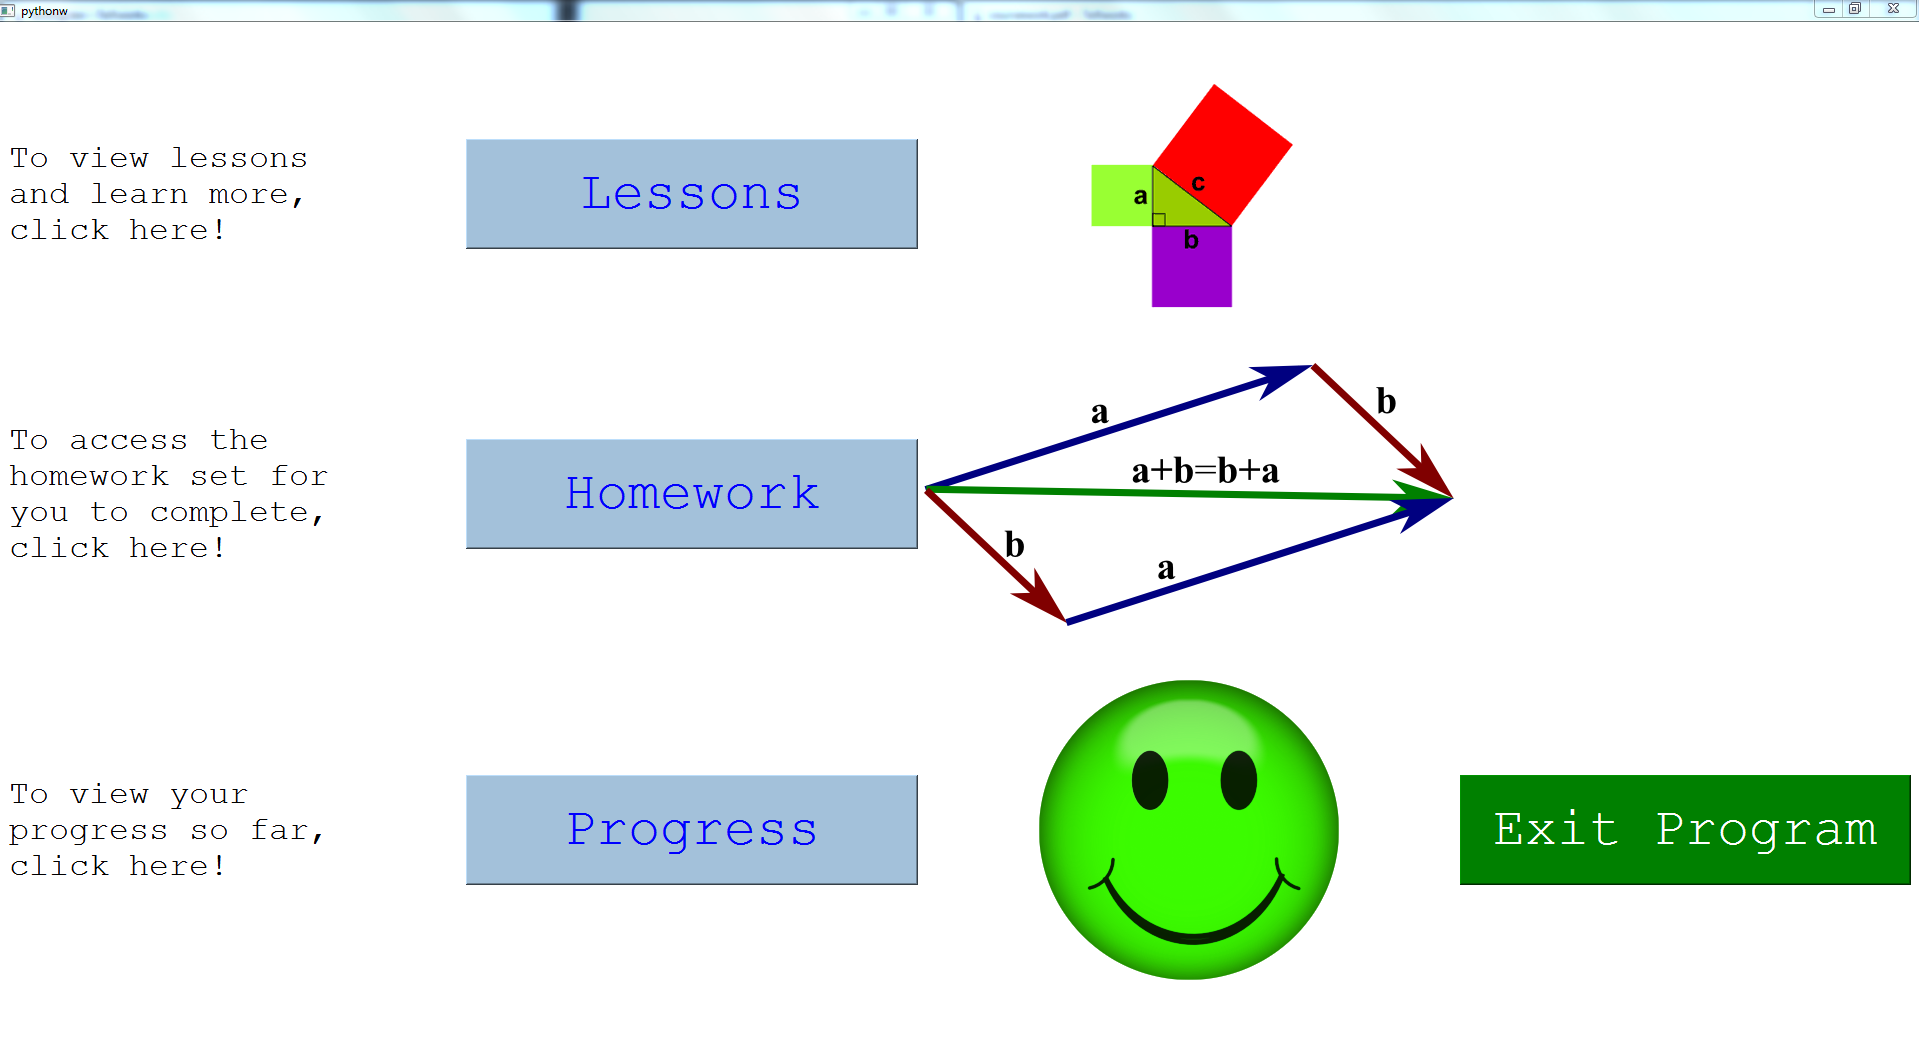
\includegraphics[width=\textwidth]{U:/git/COMP4Coursework2/Testing/screen_2}
\end{figure}

\textit{Lessons button is clicked: }

\begin{figure}[H]
    \label{fig: Second Screen}\caption{Second screen}
    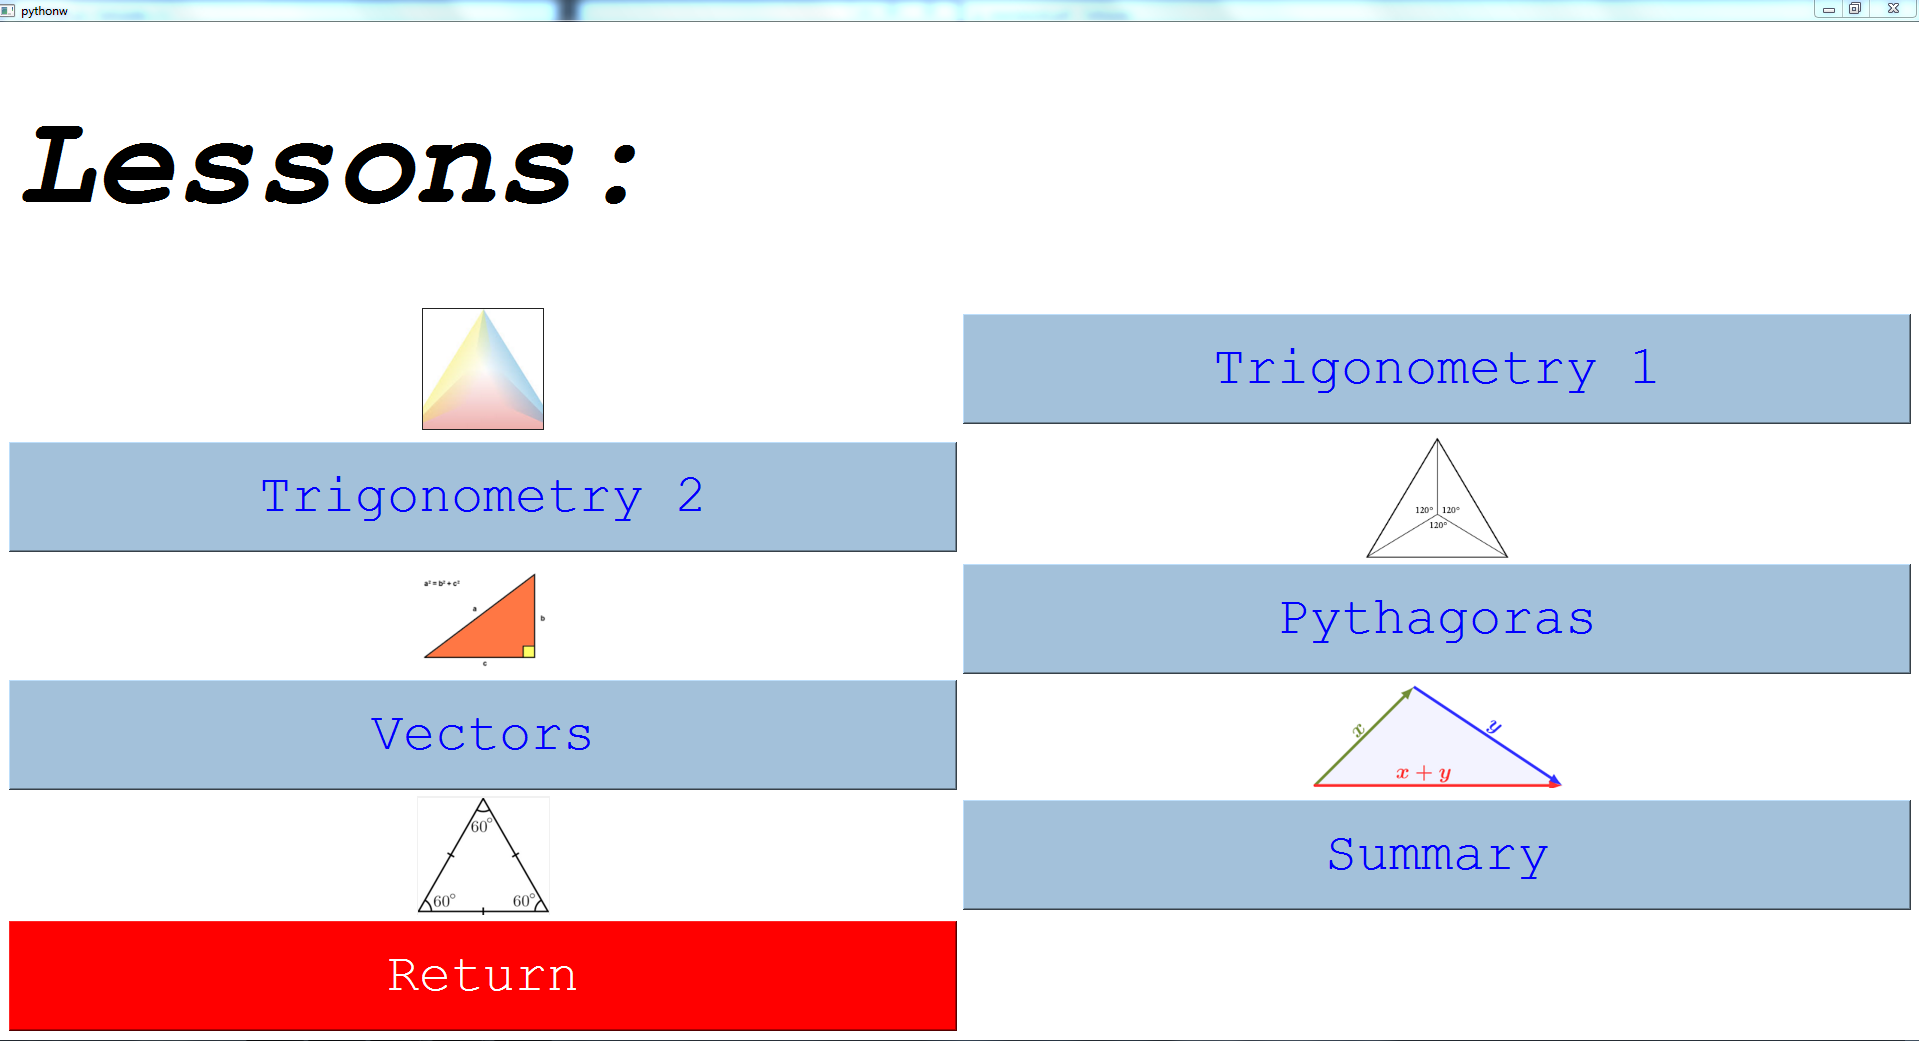
\includegraphics[width=\textwidth]{U:/git/COMP4Coursework2/Testing/screen_3}
\end{figure}

\textbf{Test 1.004}

\begin{figure}[H]
    \label{fig: First Screen}\caption{First screen}
    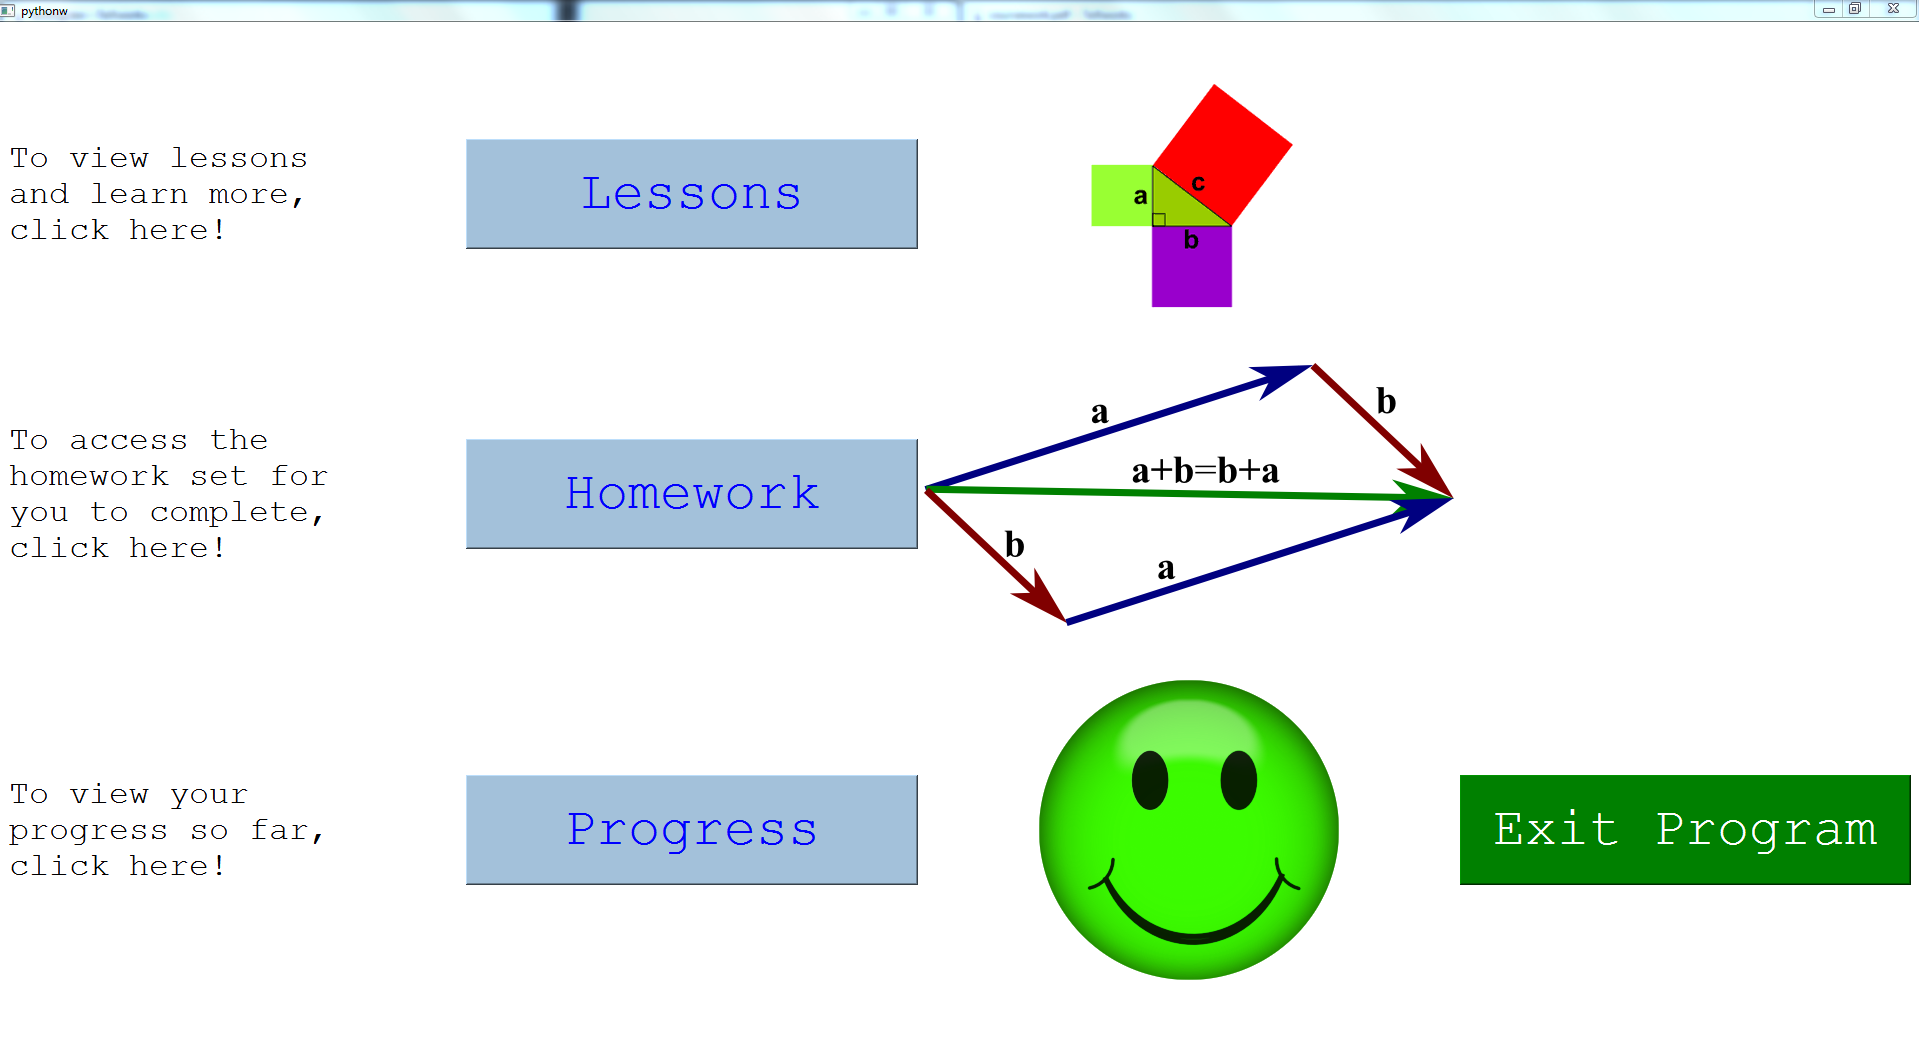
\includegraphics[width=\textwidth]{U:/git/COMP4Coursework2/Testing/screen_2}
\end{figure}

\textit{Homework button is clicked: }

\begin{figure}[H]
    \label{fig: Second Screen}\caption{Second screen}
    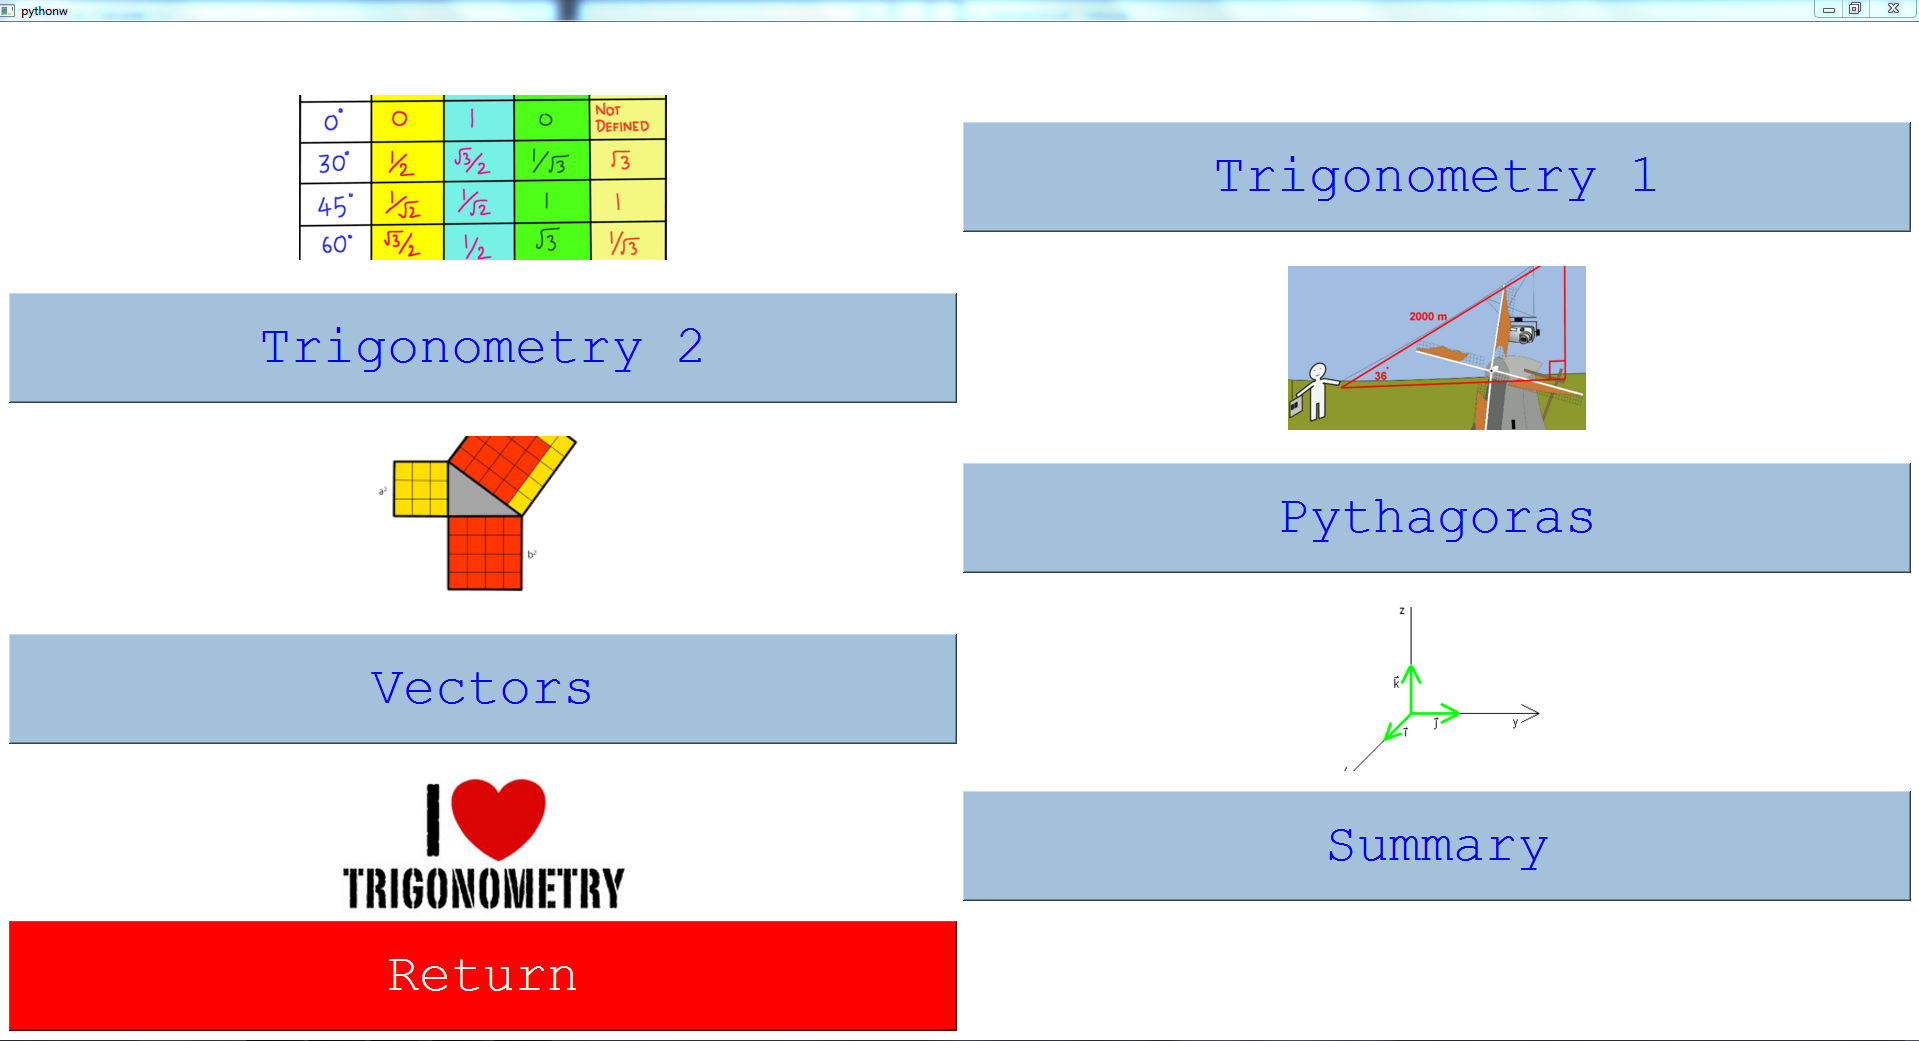
\includegraphics[width=\textwidth]{U:/git/COMP4Coursework2/Testing/screen_7}
\end{figure}

\textbf{Test 1.005}

\begin{figure}[H]
    \label{fig: First Screen}\caption{First screen}
    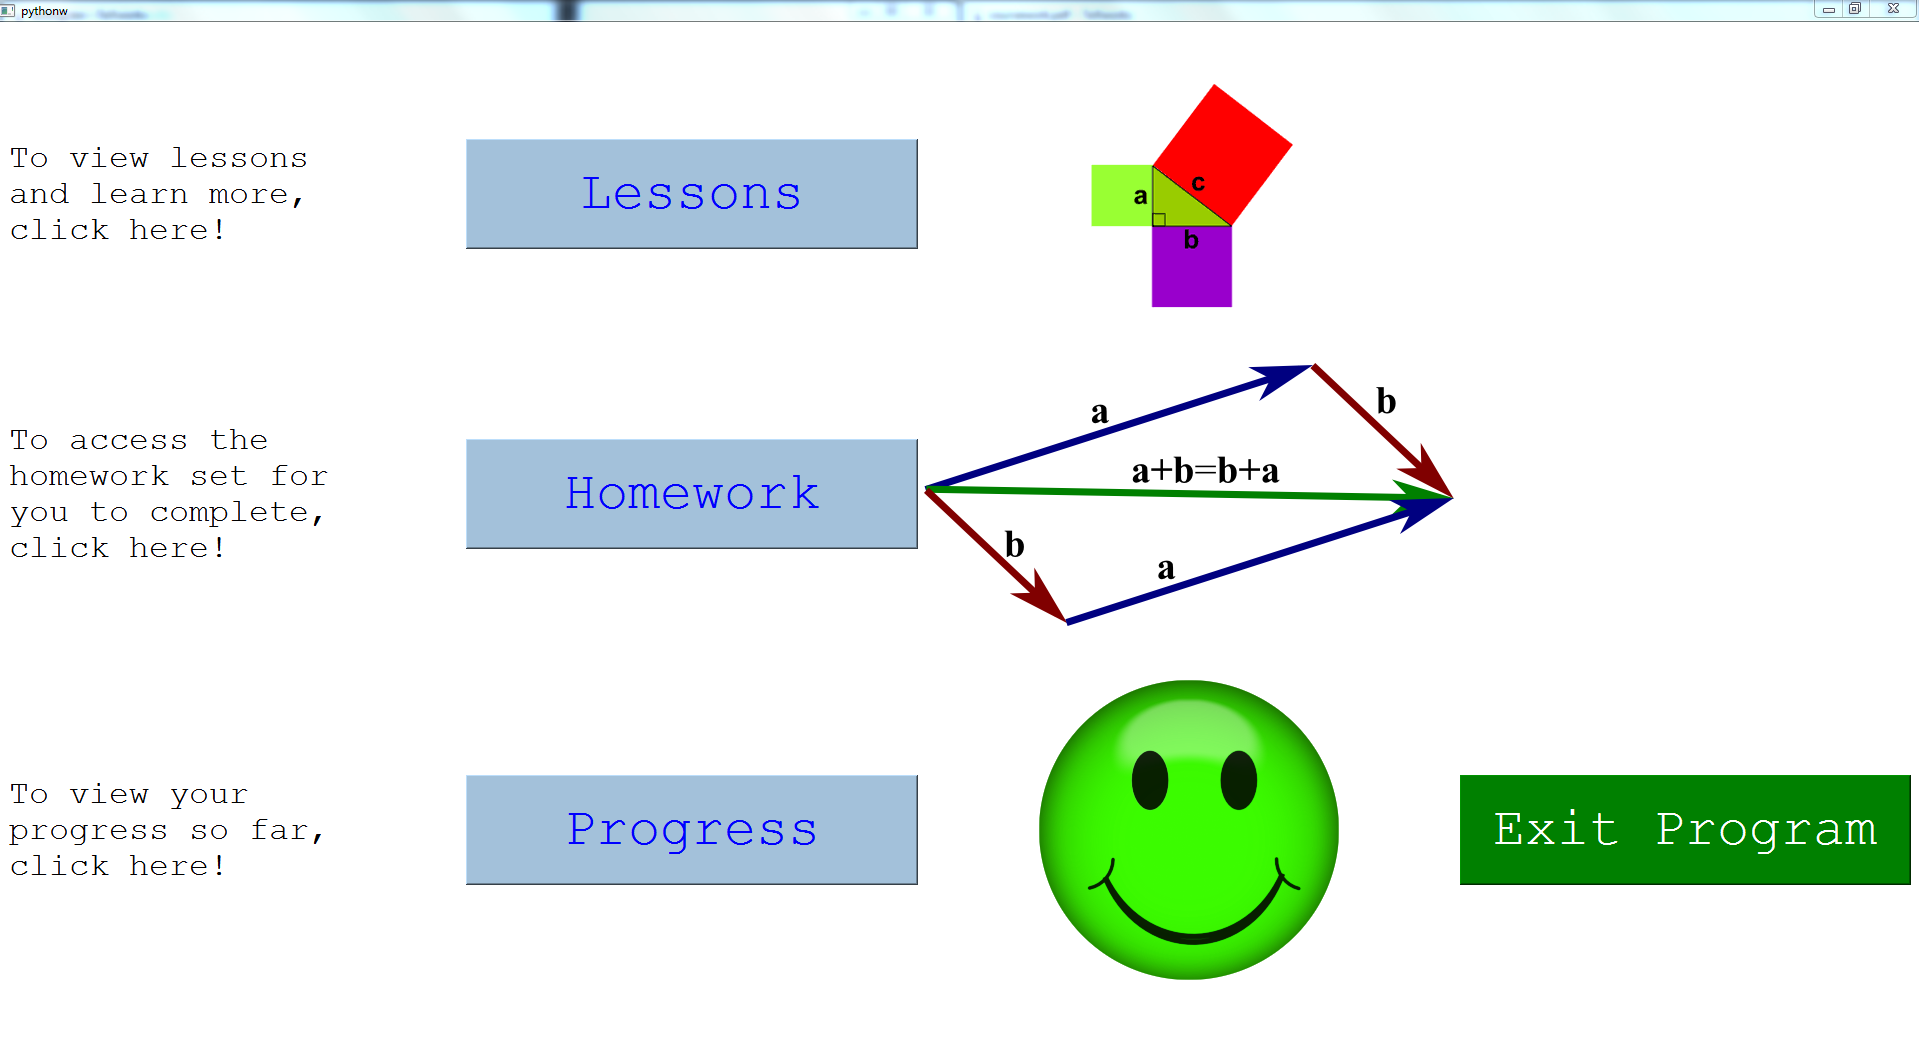
\includegraphics[width=\textwidth]{U:/git/COMP4Coursework2/Testing/screen_2}
\end{figure}

\textit{Progress button is clicked: }

\begin{figure}[H]
    \label{fig: Second Screen}\caption{Second screen}
    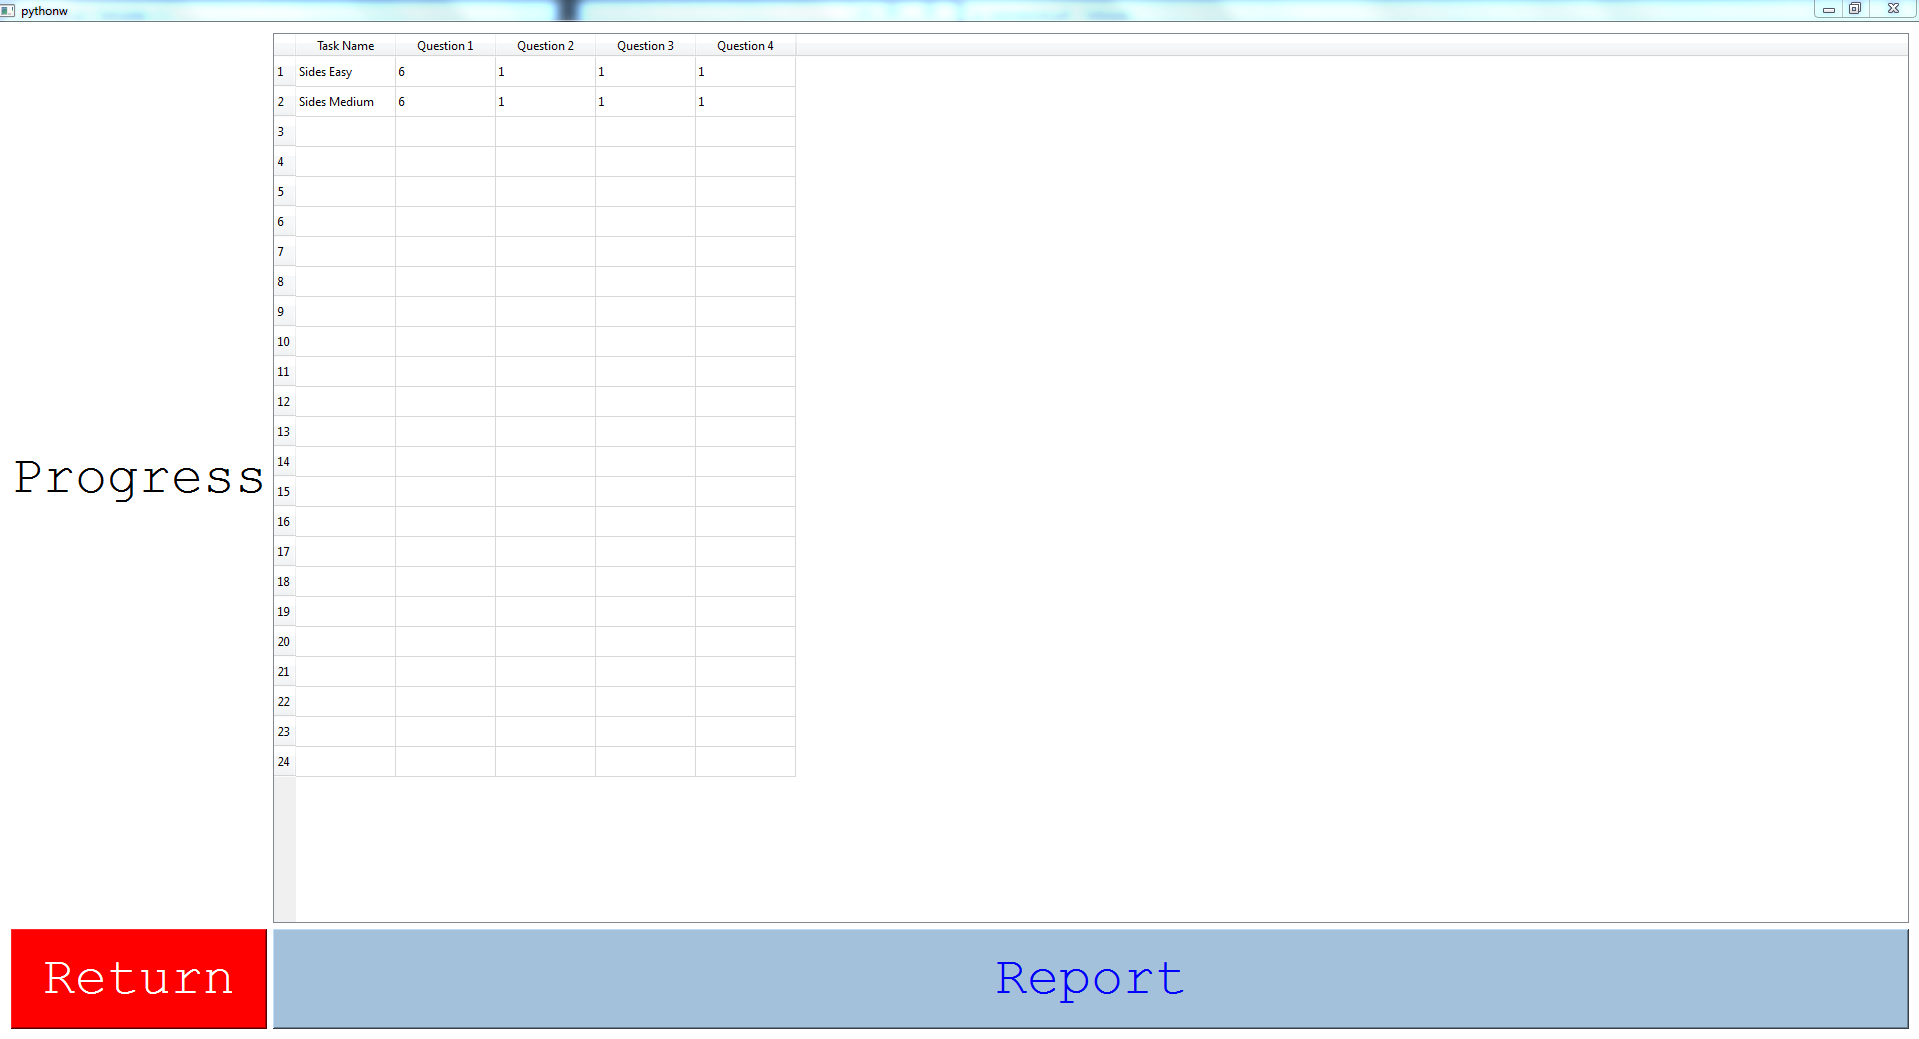
\includegraphics[width=\textwidth]{U:/git/COMP4Coursework2/Testing/screen_11}
\end{figure}

\textbf{Test 1.006}

\begin{figure}[H]
    \label{fig: First Screen}\caption{First screen}
    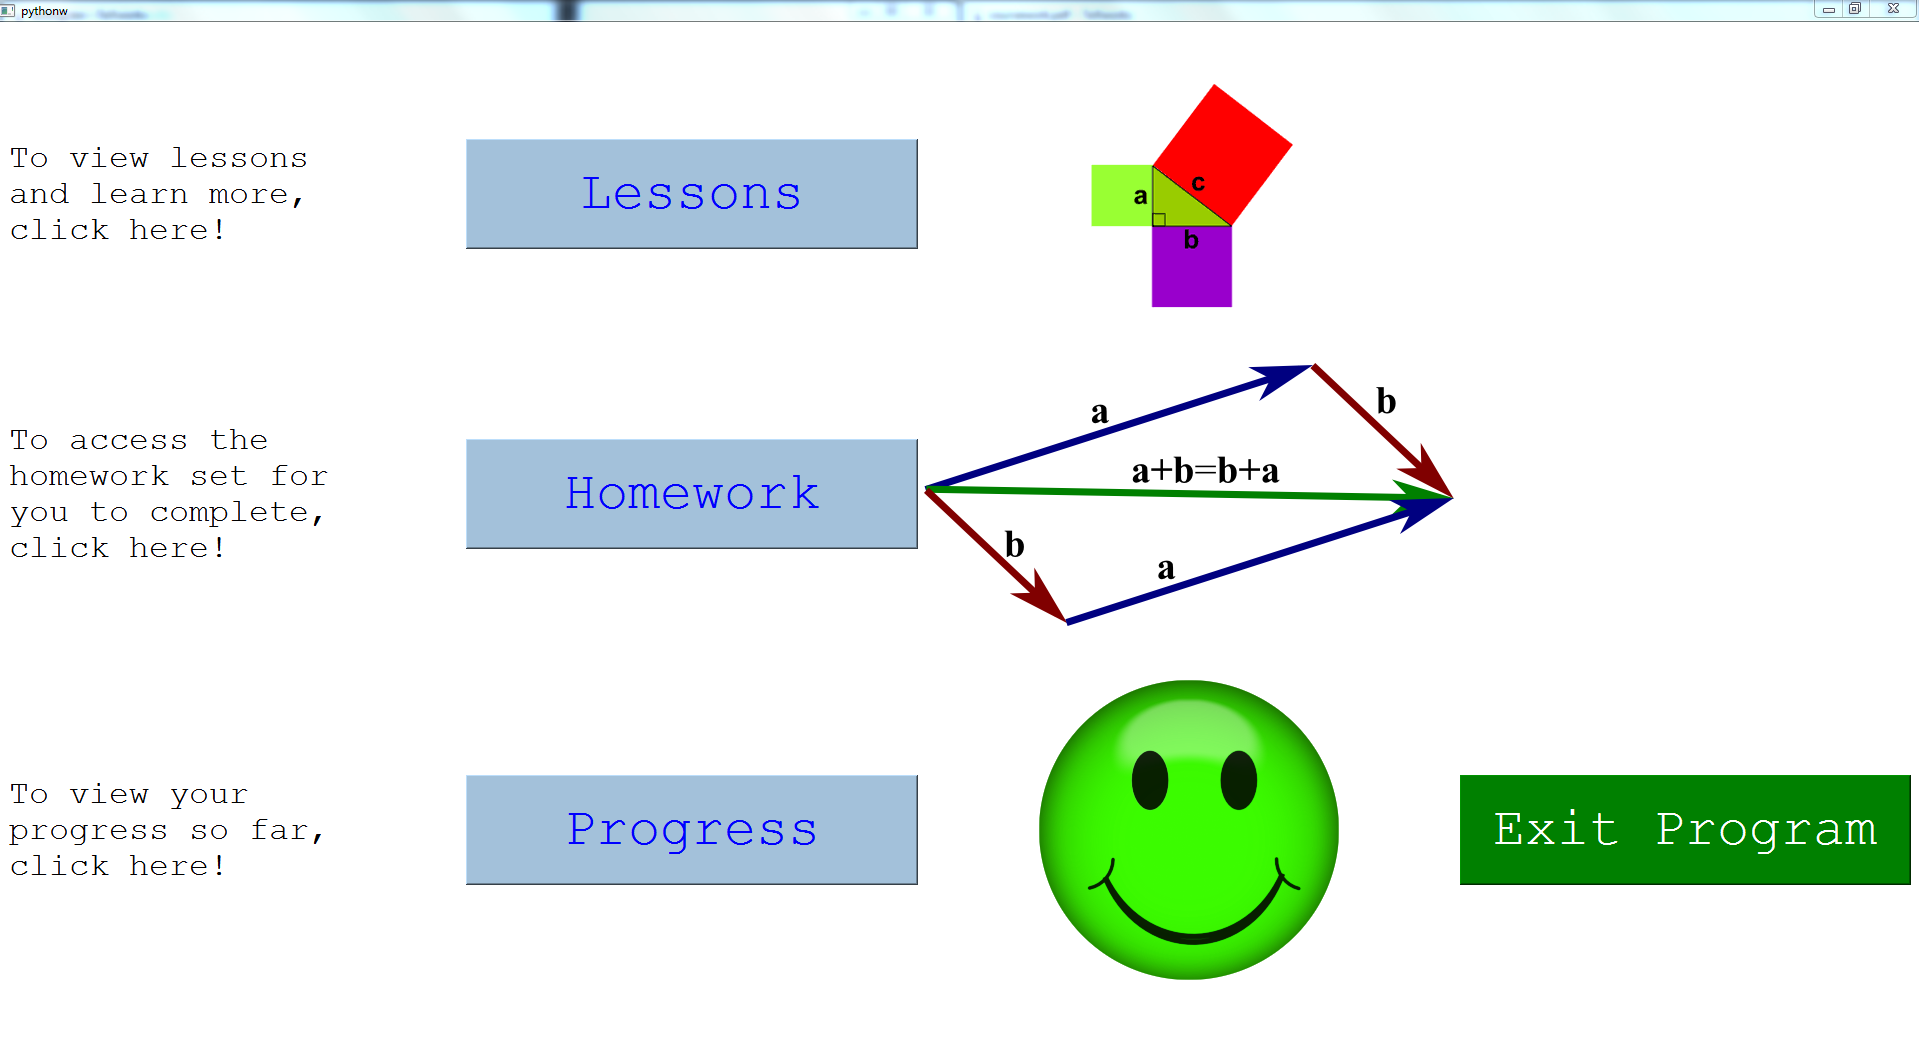
\includegraphics[width=\textwidth]{U:/git/COMP4Coursework2/Testing/screen_2}
\end{figure}

\textit{Exit program button is clicked: }

\begin{figure}[H]
    \label{fig: Second Screen}\caption{Program is closed}
    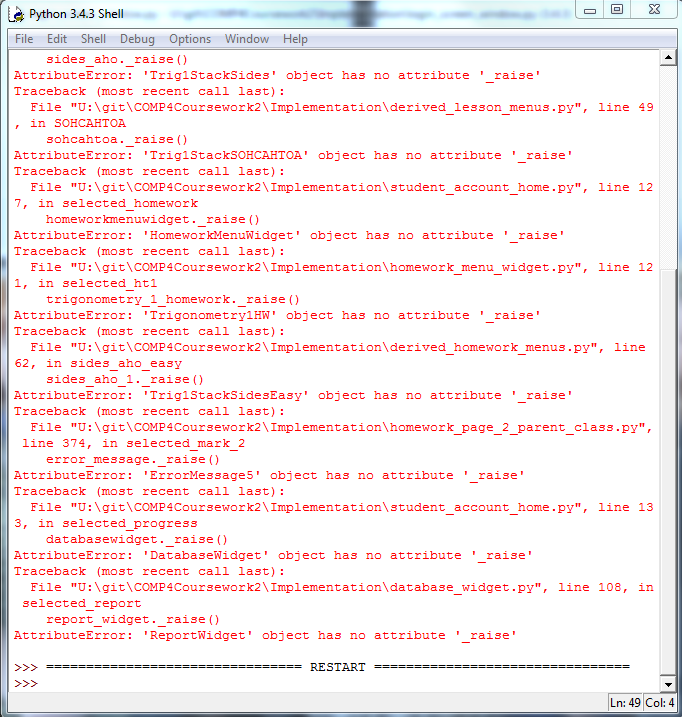
\includegraphics[width=\textwidth]{U:/git/COMP4Coursework2/Testing/screen_13}
\end{figure}

\textbf{Test 1.007}

\begin{figure}[H]
    \label{fig: First Screen}\caption{First screen}
    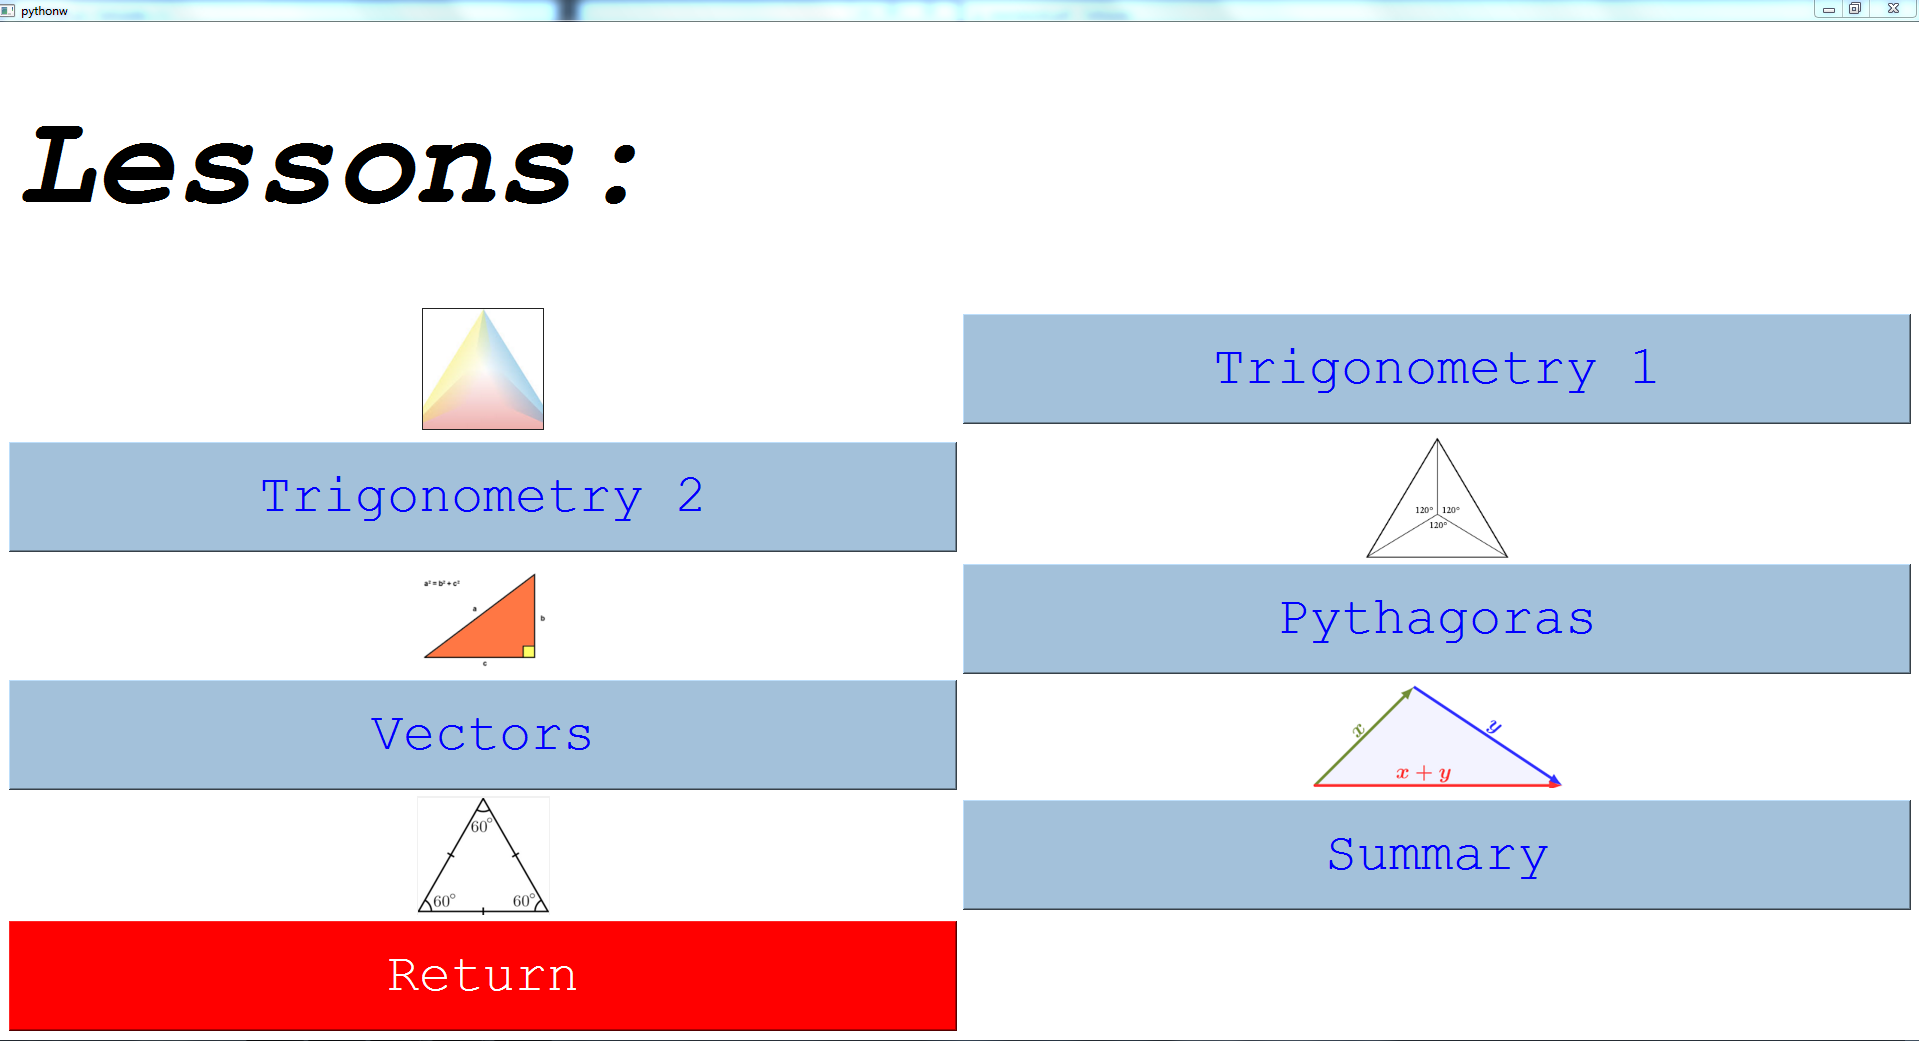
\includegraphics[width=\textwidth]{U:/git/COMP4Coursework2/Testing/screen_3}
\end{figure}

\textit{Trigonometry 1 button is clicked: }

\begin{figure}[H]
    \label{fig: Second Screen}\caption{Second screen}
    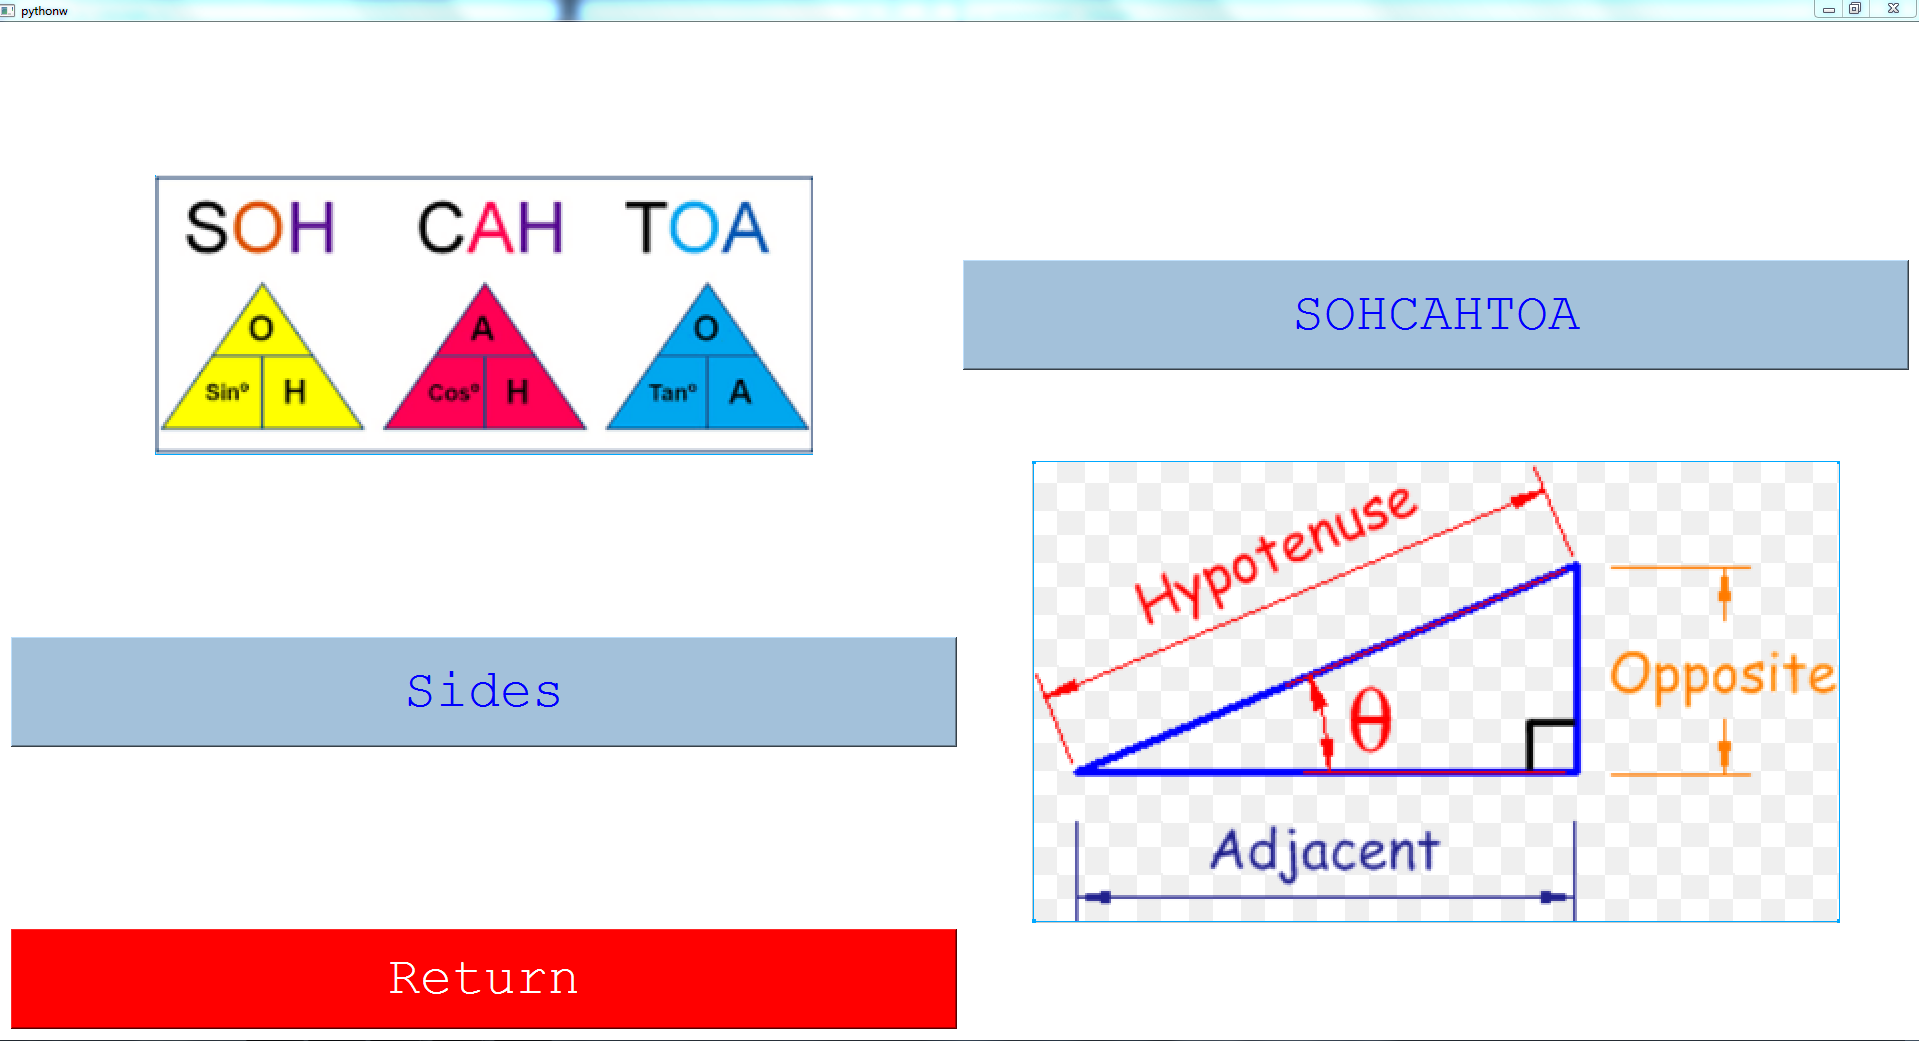
\includegraphics[width=\textwidth]{U:/git/COMP4Coursework2/Testing/screen_4}
\end{figure}

\textbf{Test 1.012}

\begin{figure}[H]
    \label{fig: First Screen}\caption{First screen}
    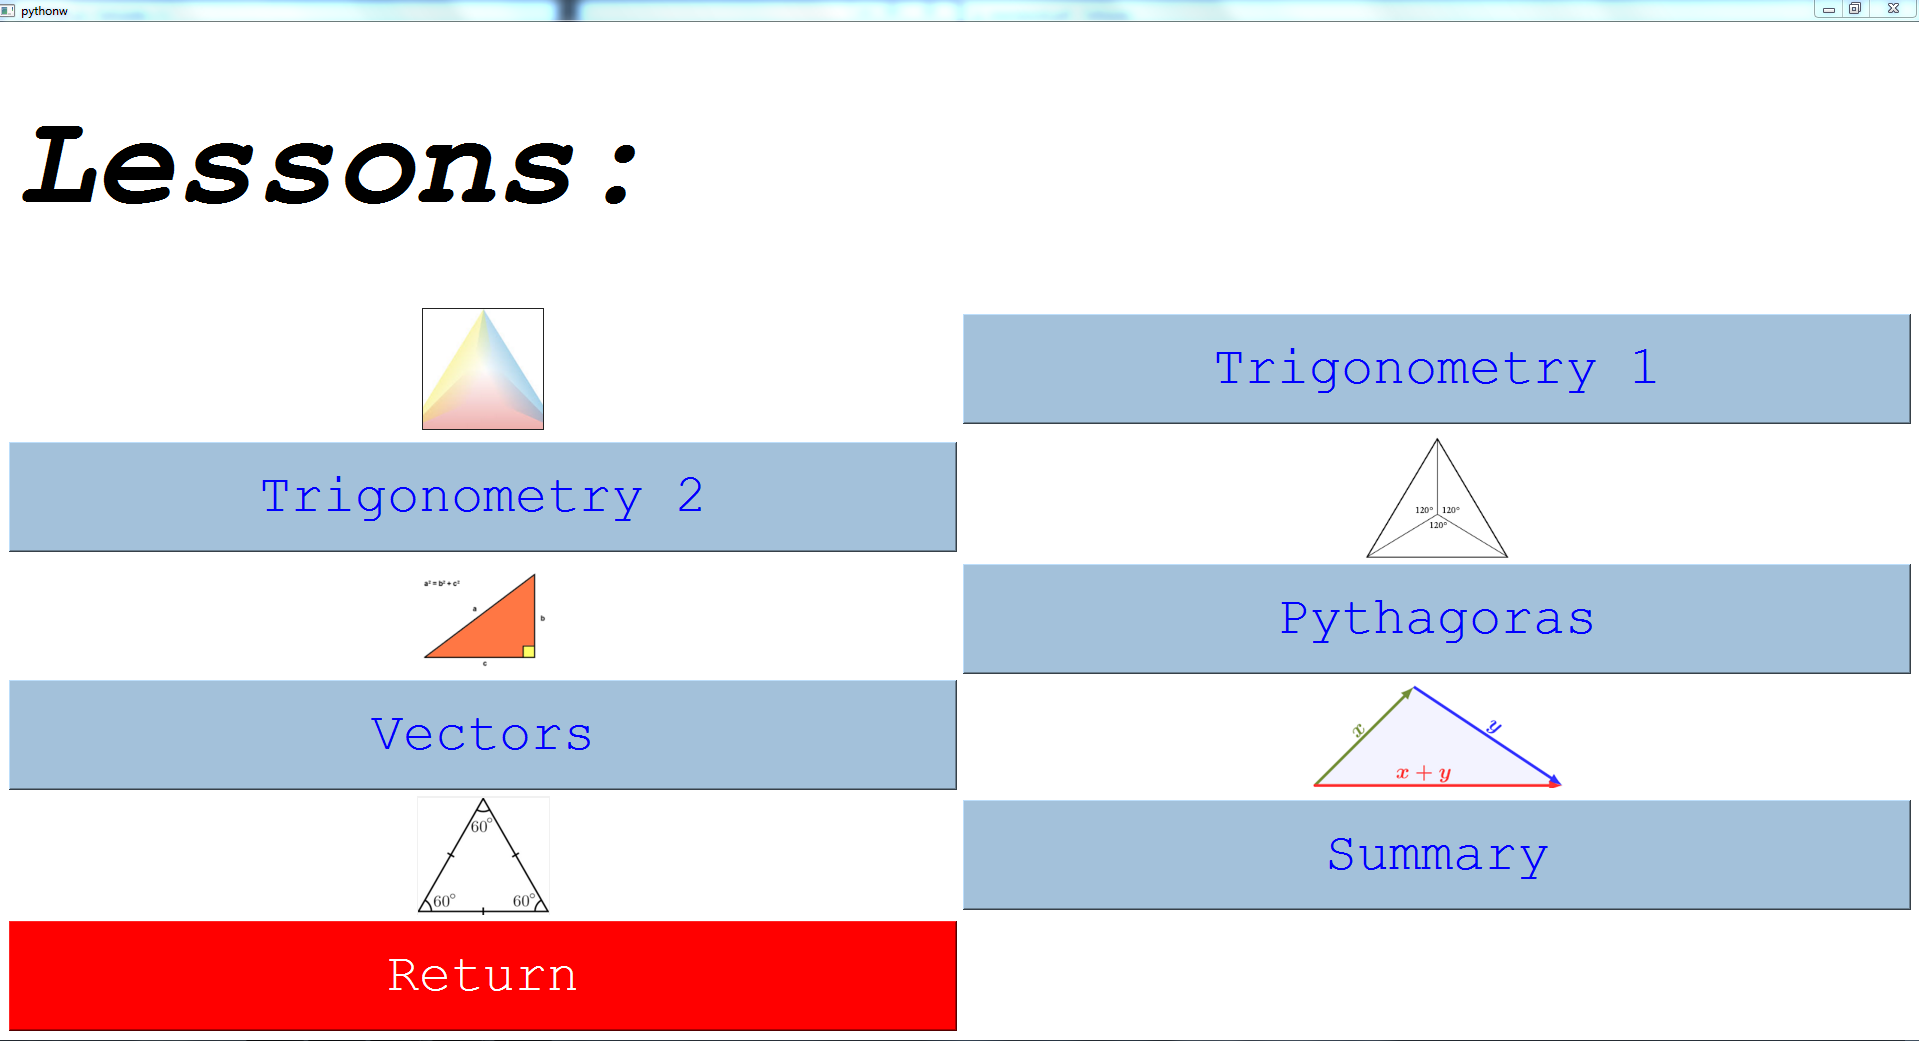
\includegraphics[width=\textwidth]{U:/git/COMP4Coursework2/Testing/screen_3}
\end{figure}

\textit{Return button is clicked: }

\begin{figure}[H]
    \label{fig: Second Screen}\caption{Second screen}
    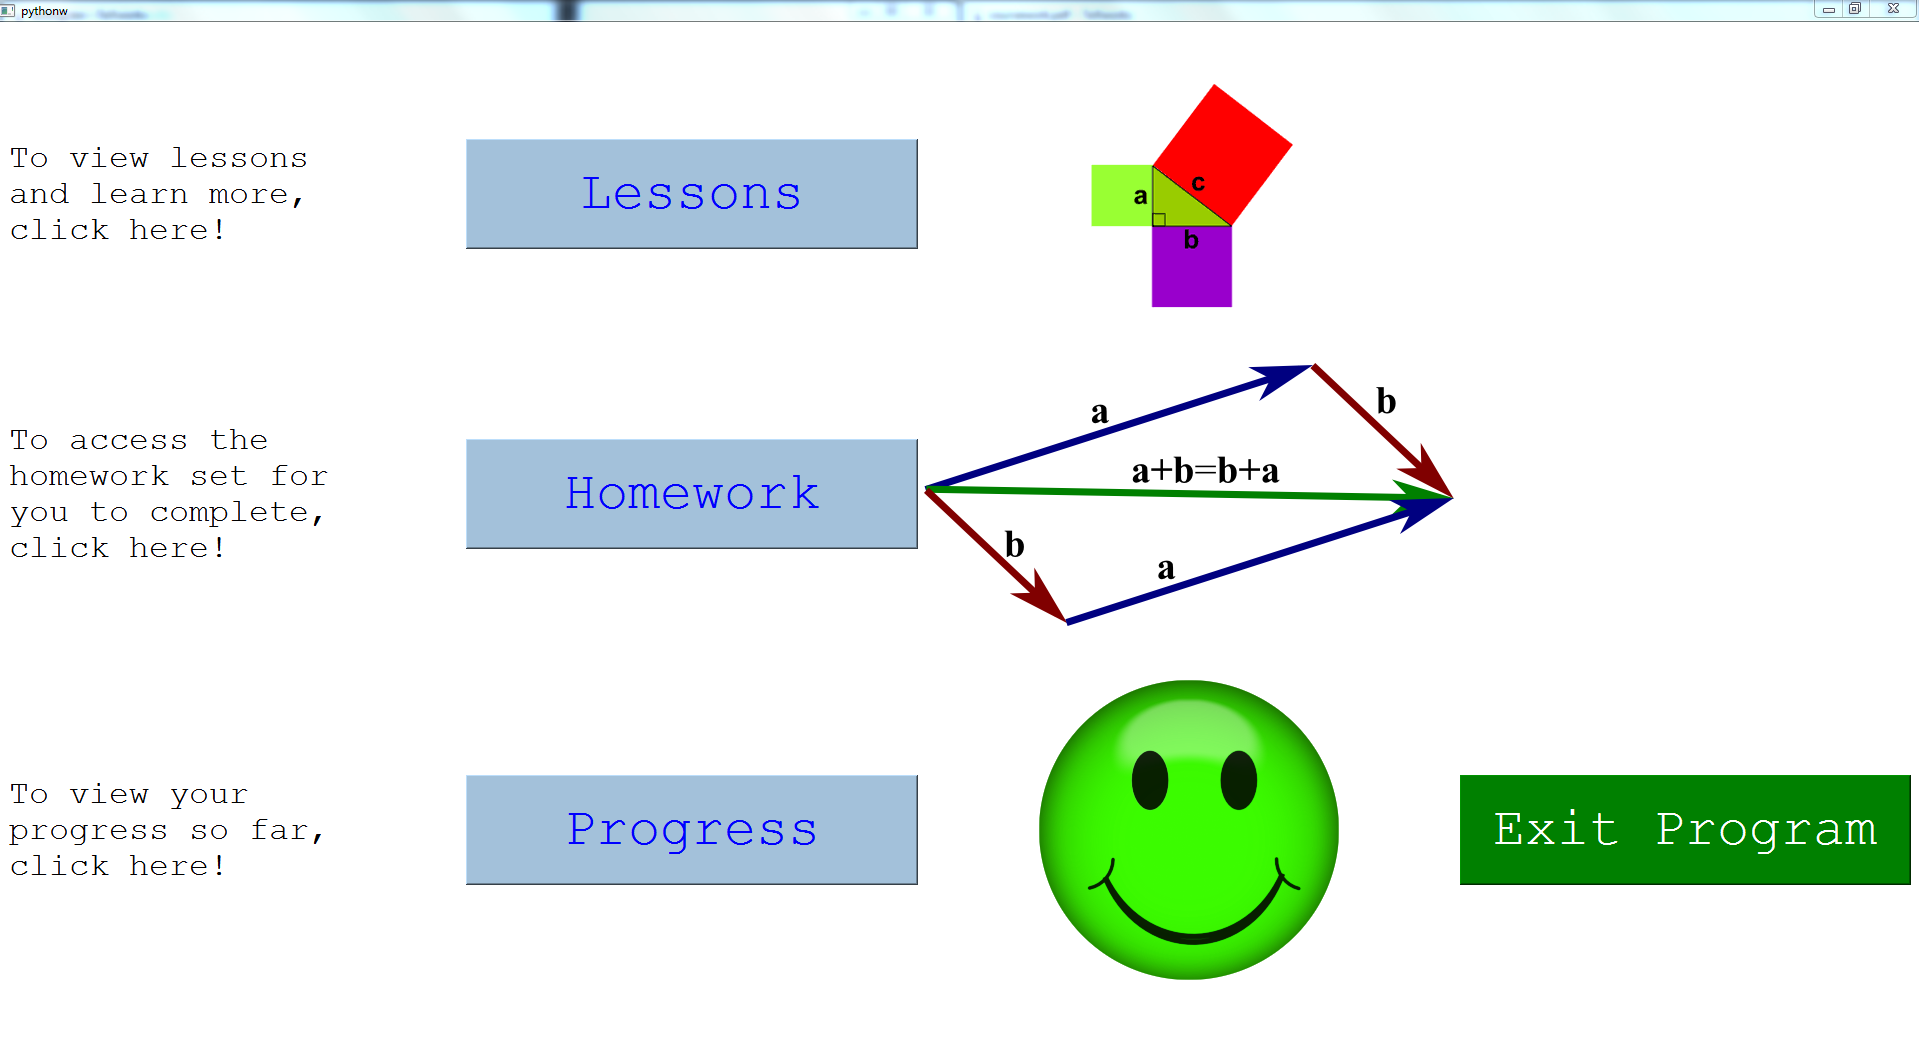
\includegraphics[width=\textwidth]{U:/git/COMP4Coursework2/Testing/screen_2}
\end{figure}

\textbf{Test 1.013}

\begin{figure}[H]
    \label{fig: First Screen}\caption{First screen}
    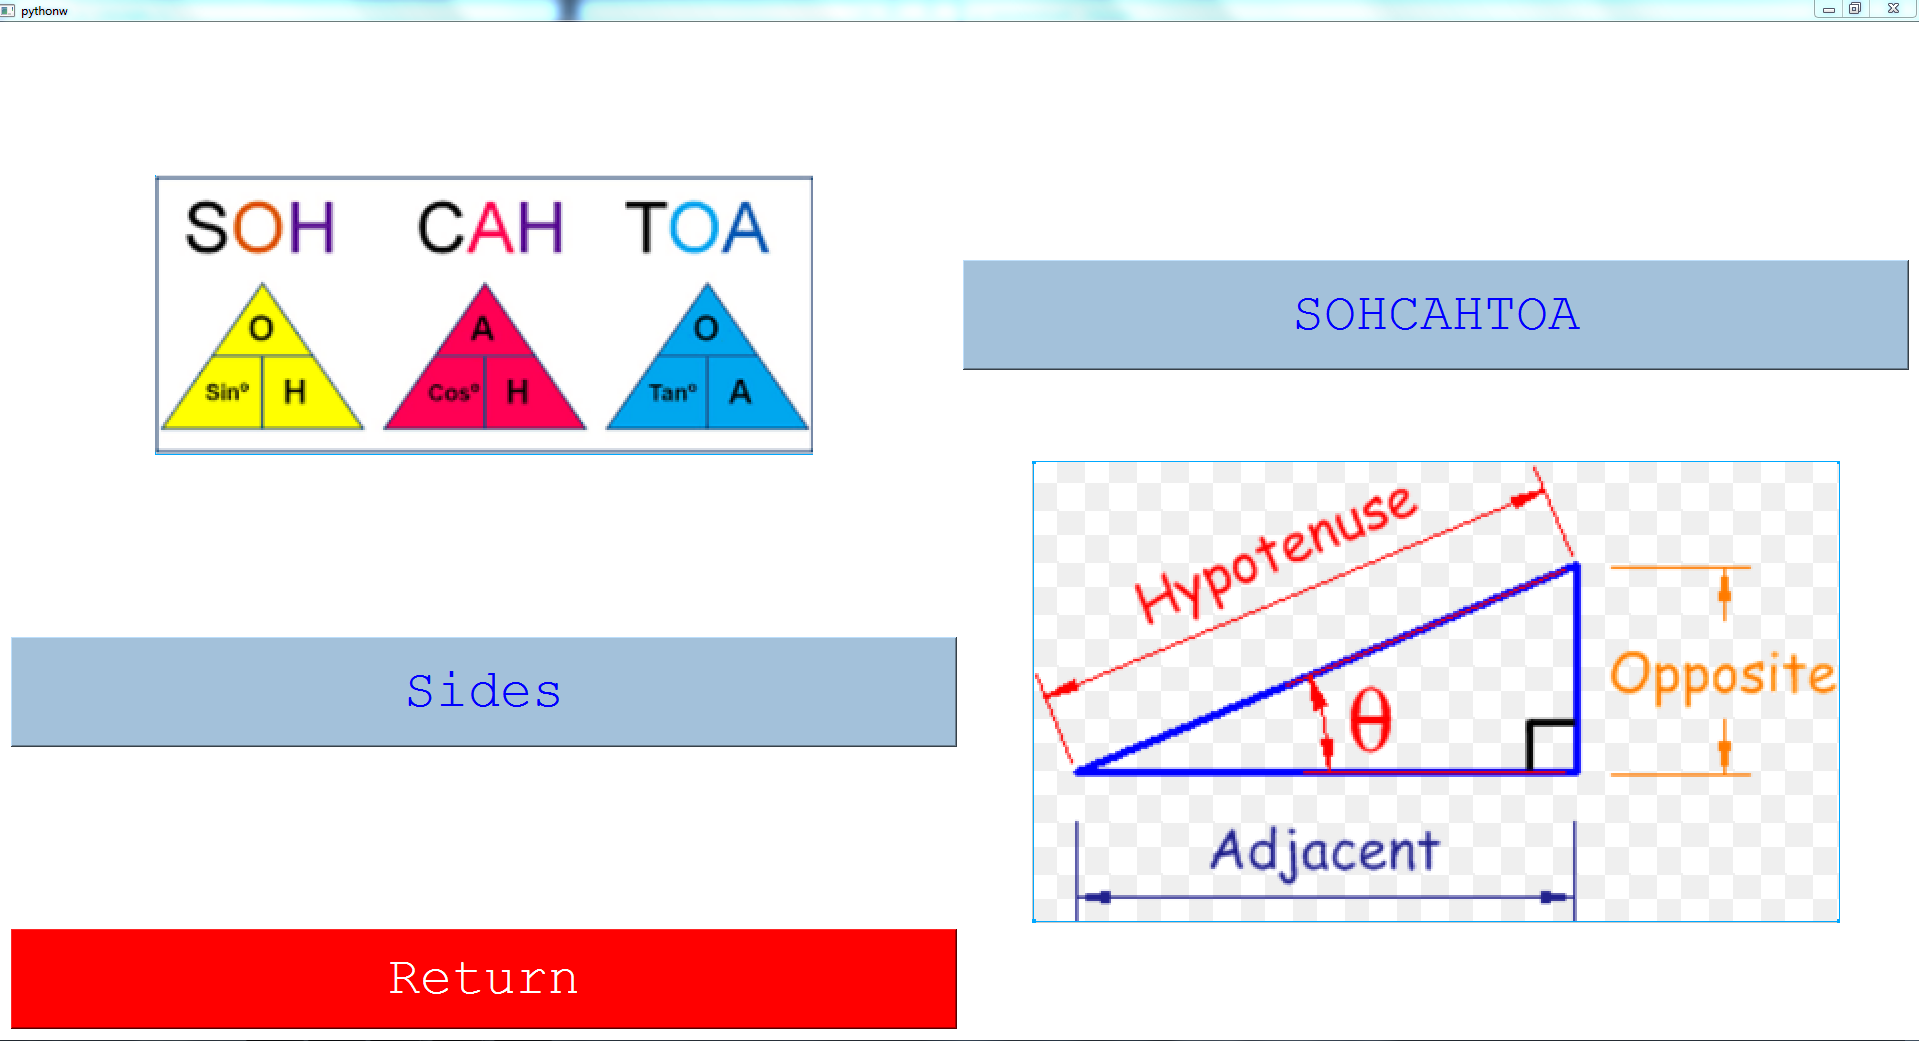
\includegraphics[width=\textwidth]{U:/git/COMP4Coursework2/Testing/screen_4}
\end{figure}

\textit{Sides button is clicked: }

\begin{figure}[H]
    \label{fig: Second Screen}\caption{Second screen}
    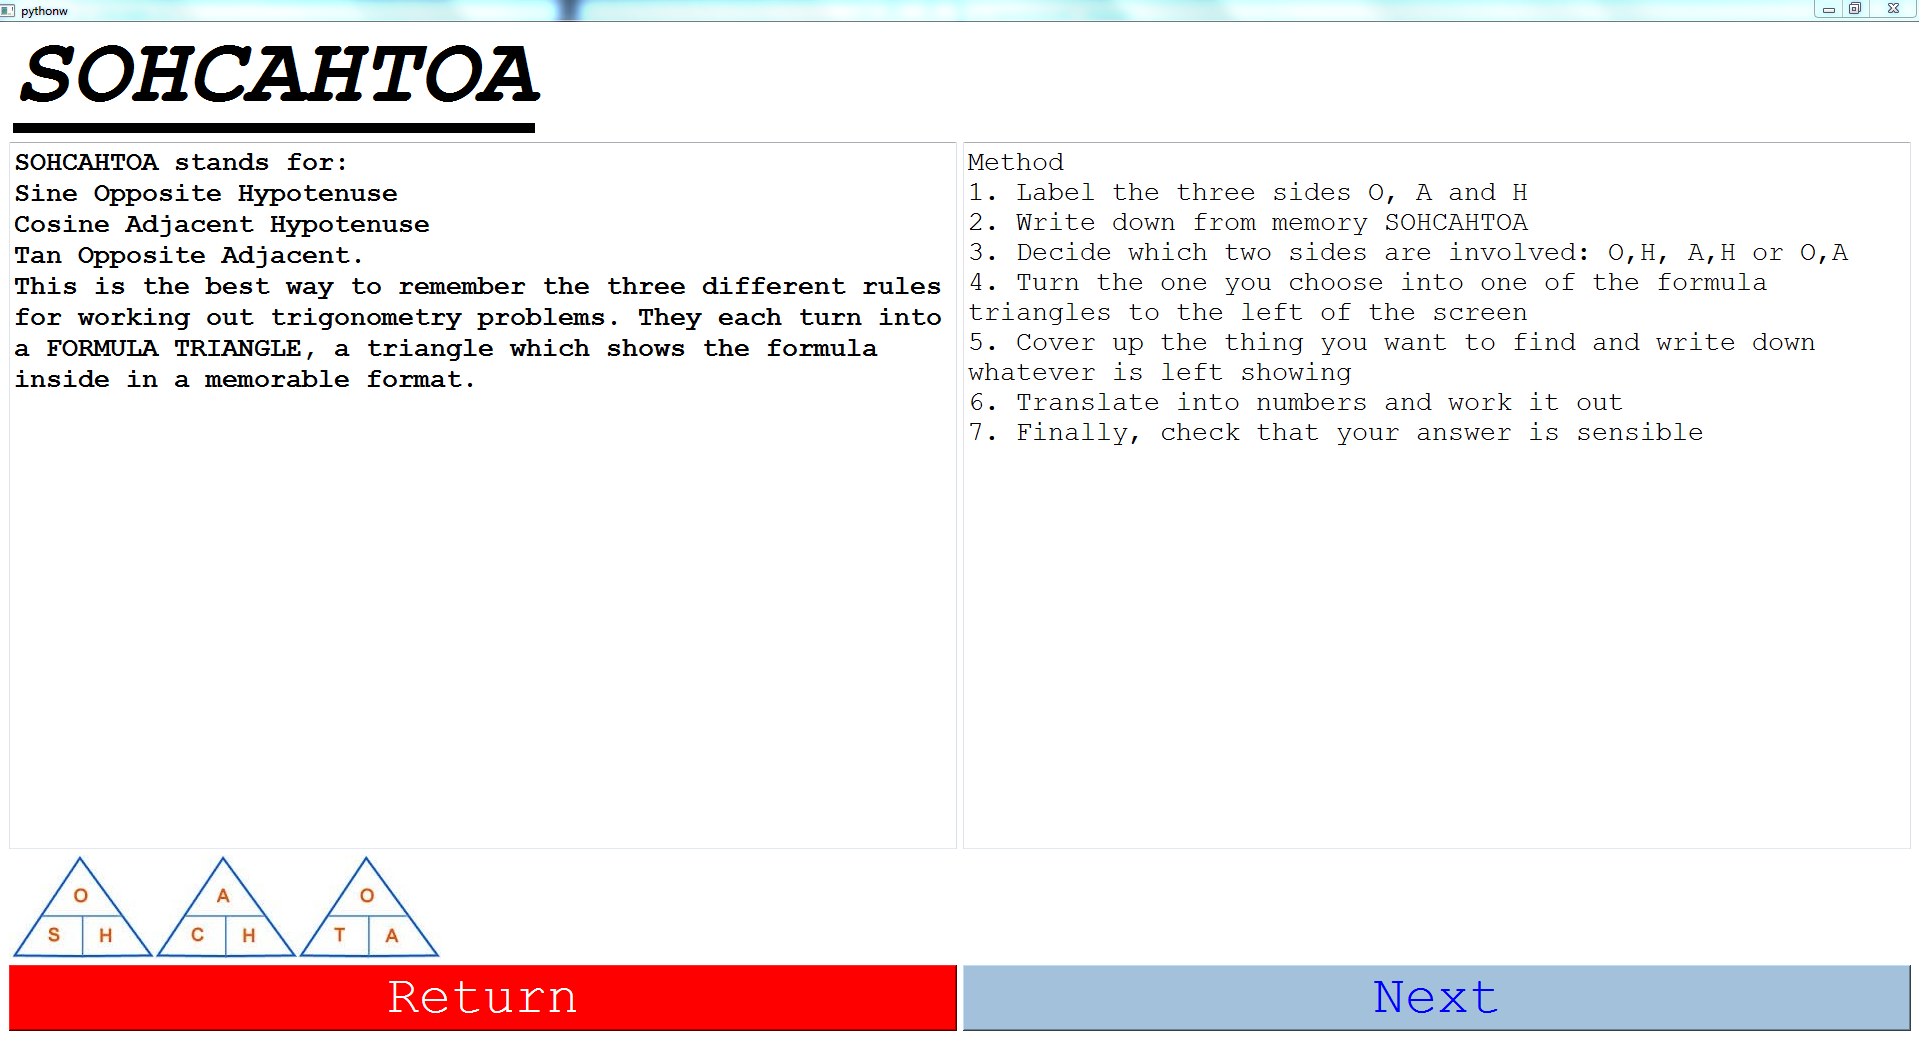
\includegraphics[width=\textwidth]{U:/git/COMP4Coursework2/Testing/screen_5}
\end{figure}

\textbf{Test 1.015}

\begin{figure}[H]
    \label{fig: First Screen}\caption{First screen}
    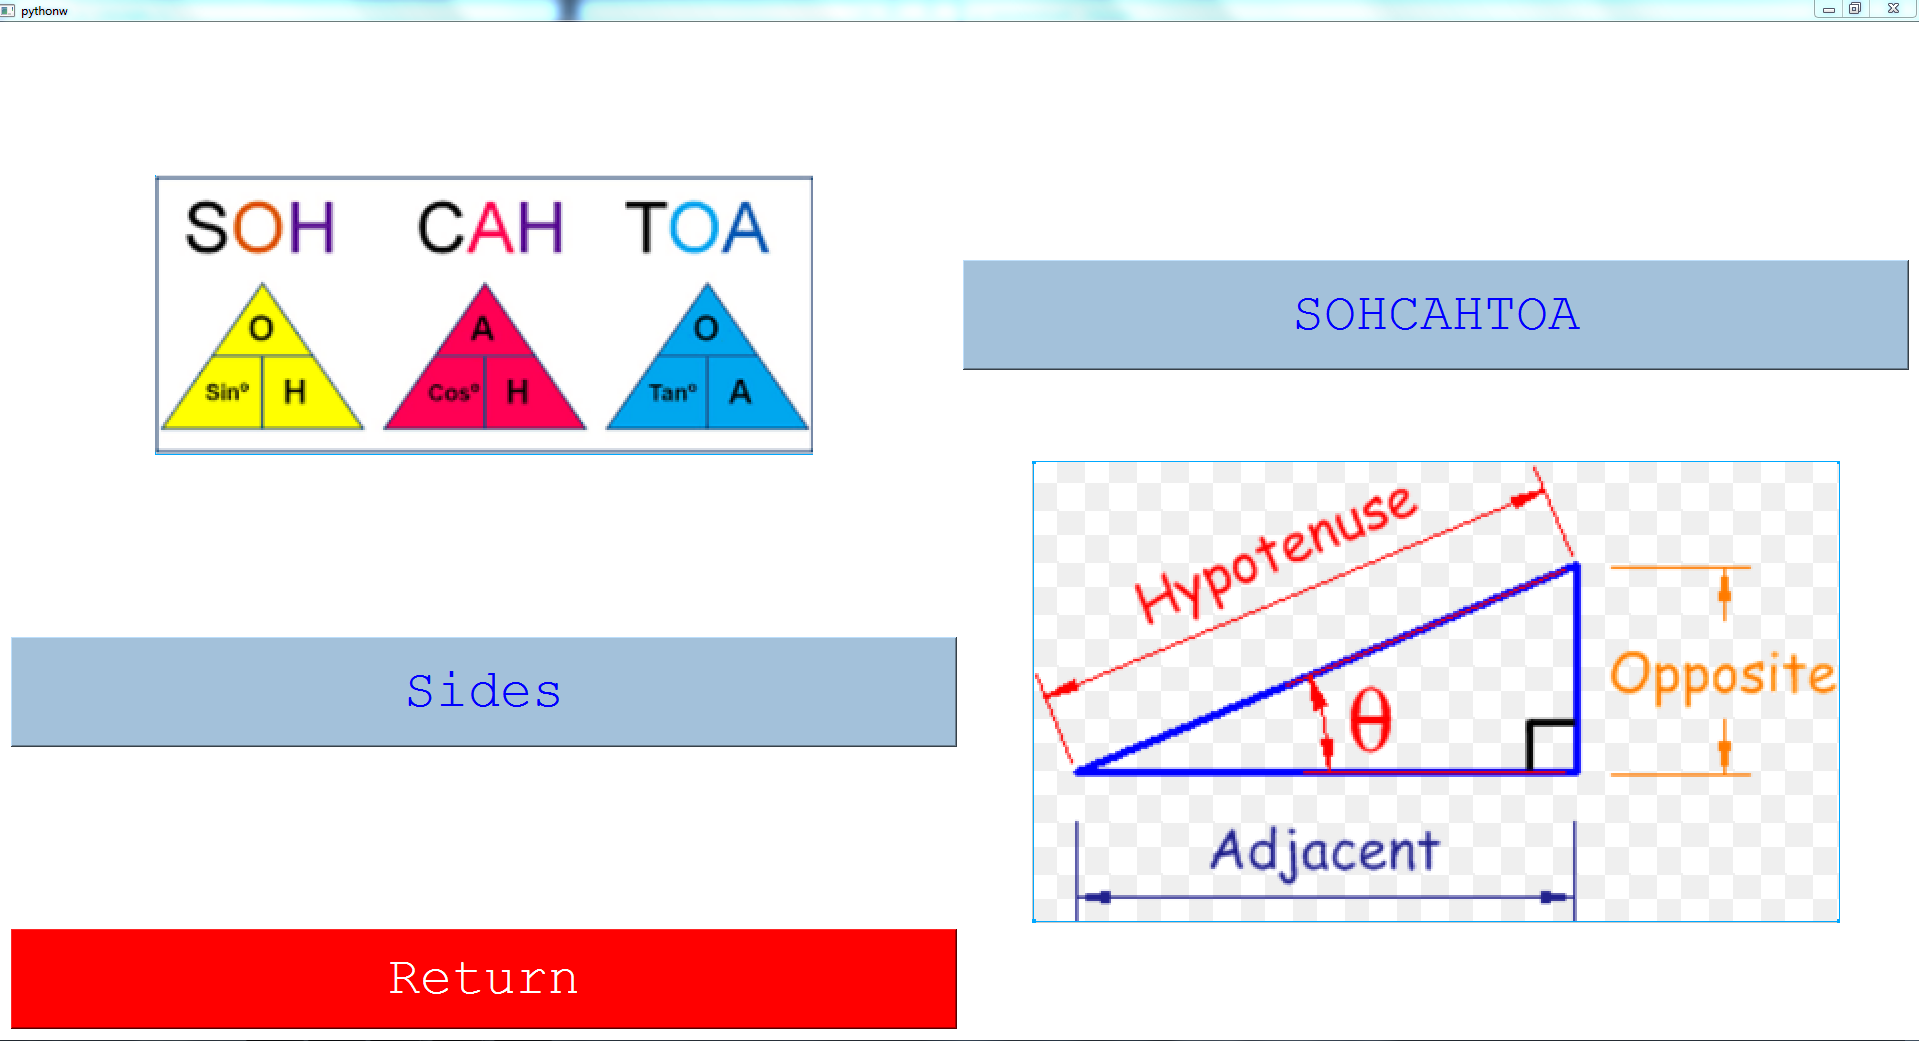
\includegraphics[width=\textwidth]{U:/git/COMP4Coursework2/Testing/screen_4}
\end{figure}

\textit{Return button is clicked: }

\begin{figure}[H]
    \label{fig: Second Screen}\caption{Second screen}
    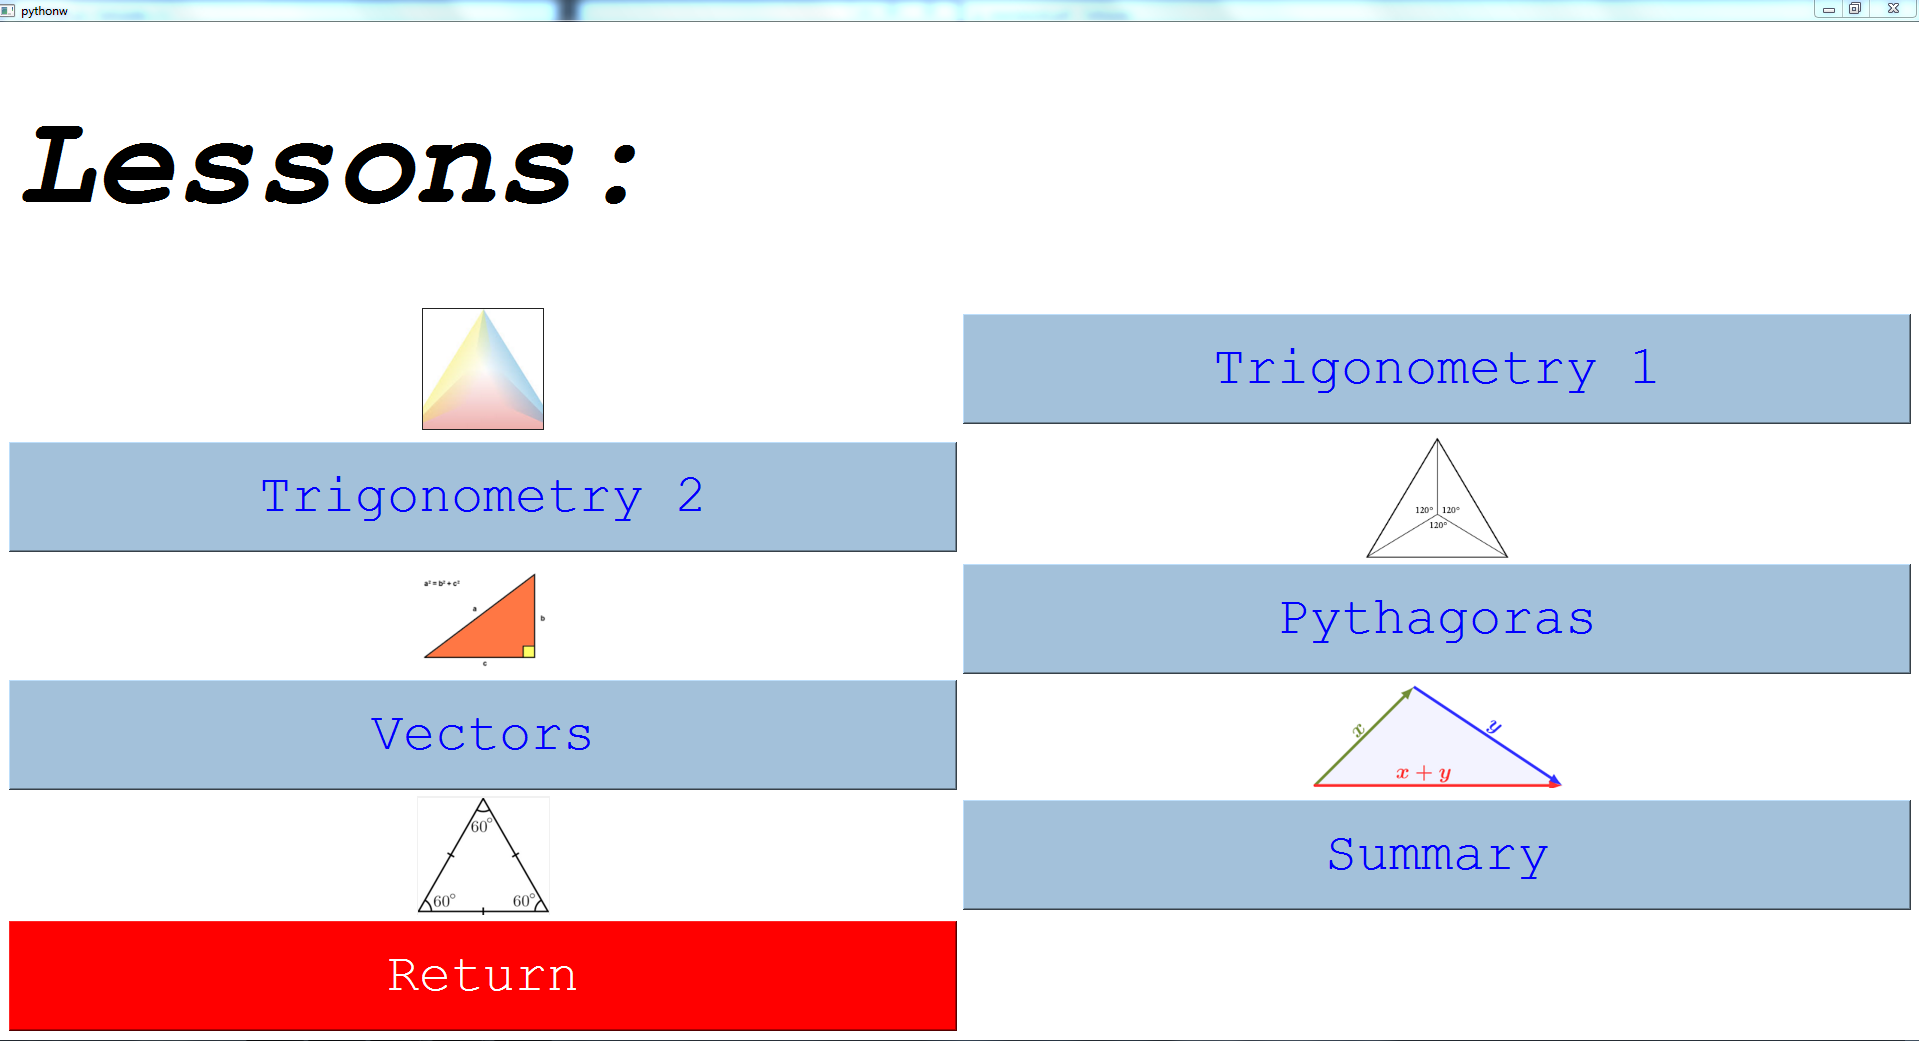
\includegraphics[width=\textwidth]{U:/git/COMP4Coursework2/Testing/screen_3}
\end{figure}

\textbf{Test 1.031}

\begin{figure}[H]
    \label{fig: First Screen}\caption{First screen}
    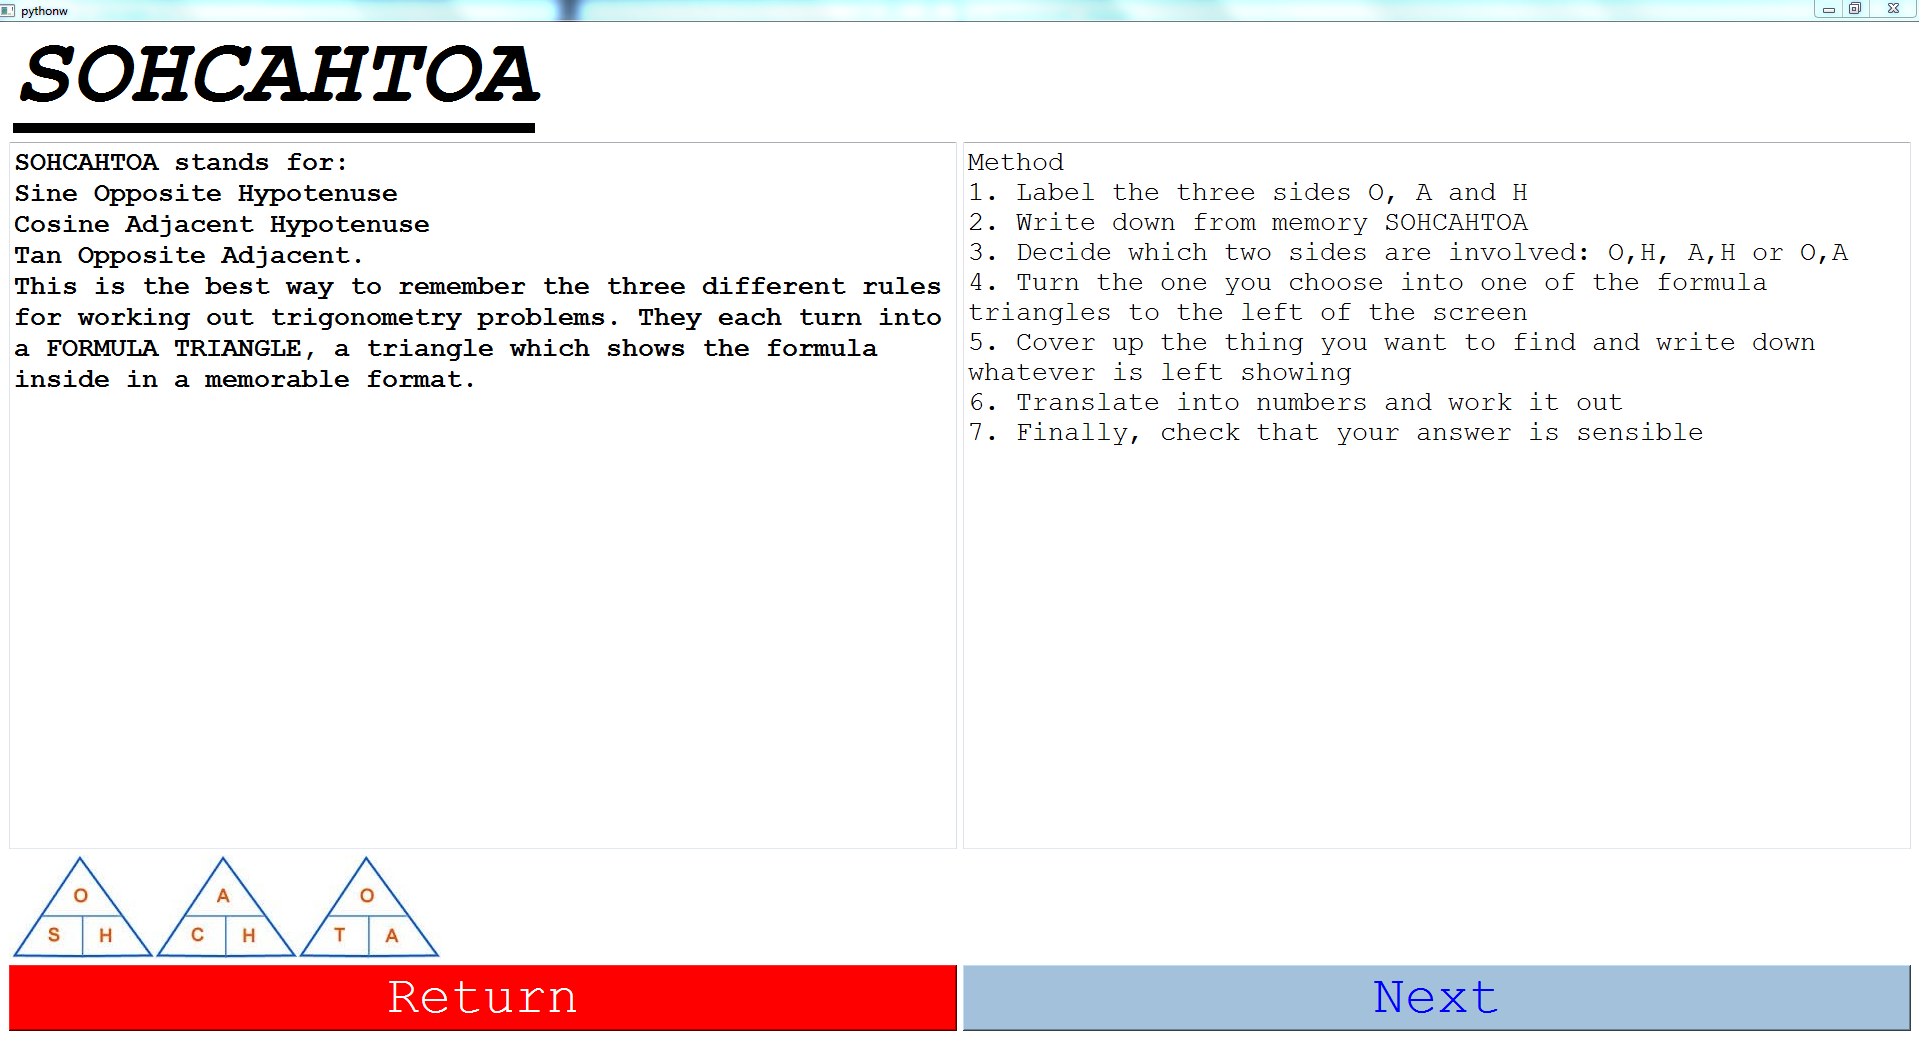
\includegraphics[width=\textwidth]{U:/git/COMP4Coursework2/Testing/screen_5}
\end{figure}

\textit{Return button is clicked: }

\begin{figure}[H]
    \label{fig: Second Screen}\caption{Second screen}
    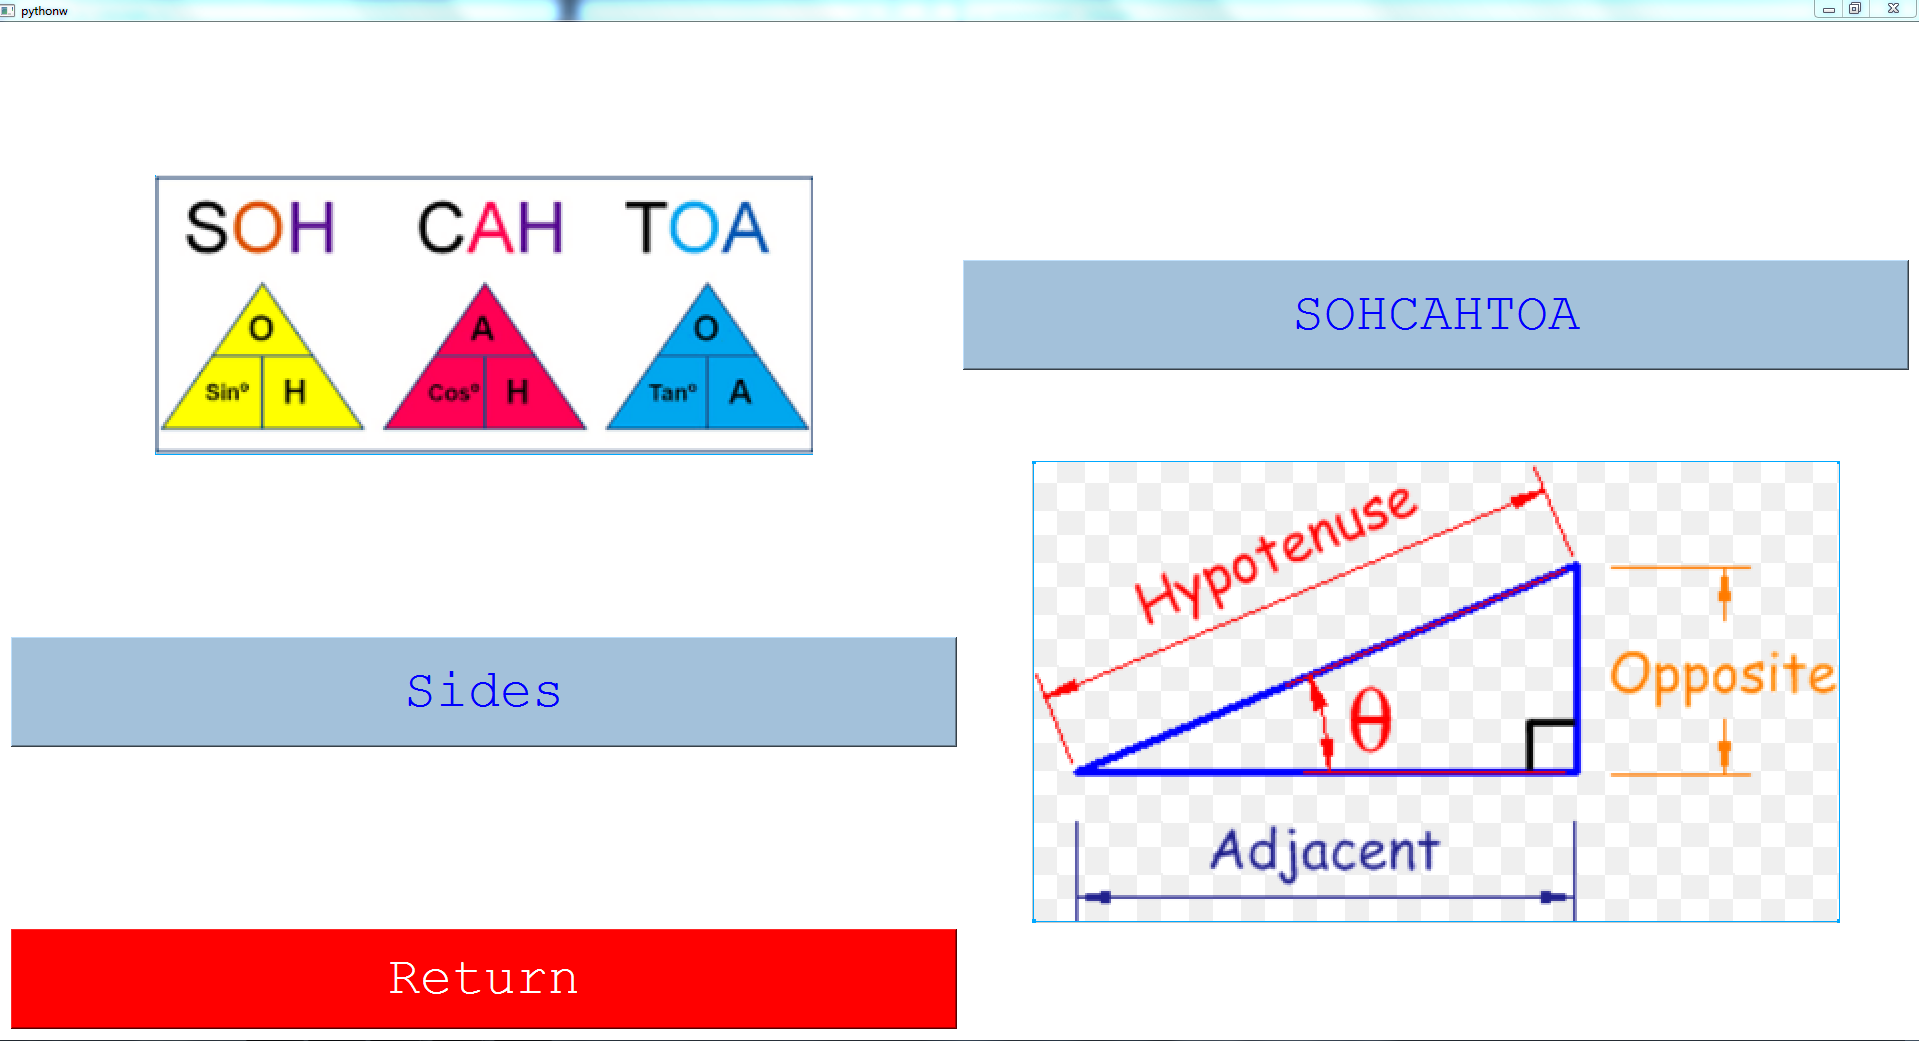
\includegraphics[width=\textwidth]{U:/git/COMP4Coursework2/Testing/screen_4}
\end{figure}

\textbf{Test 1.032}

\begin{figure}[H]
    \label{fig: First Screen}\caption{First screen}
    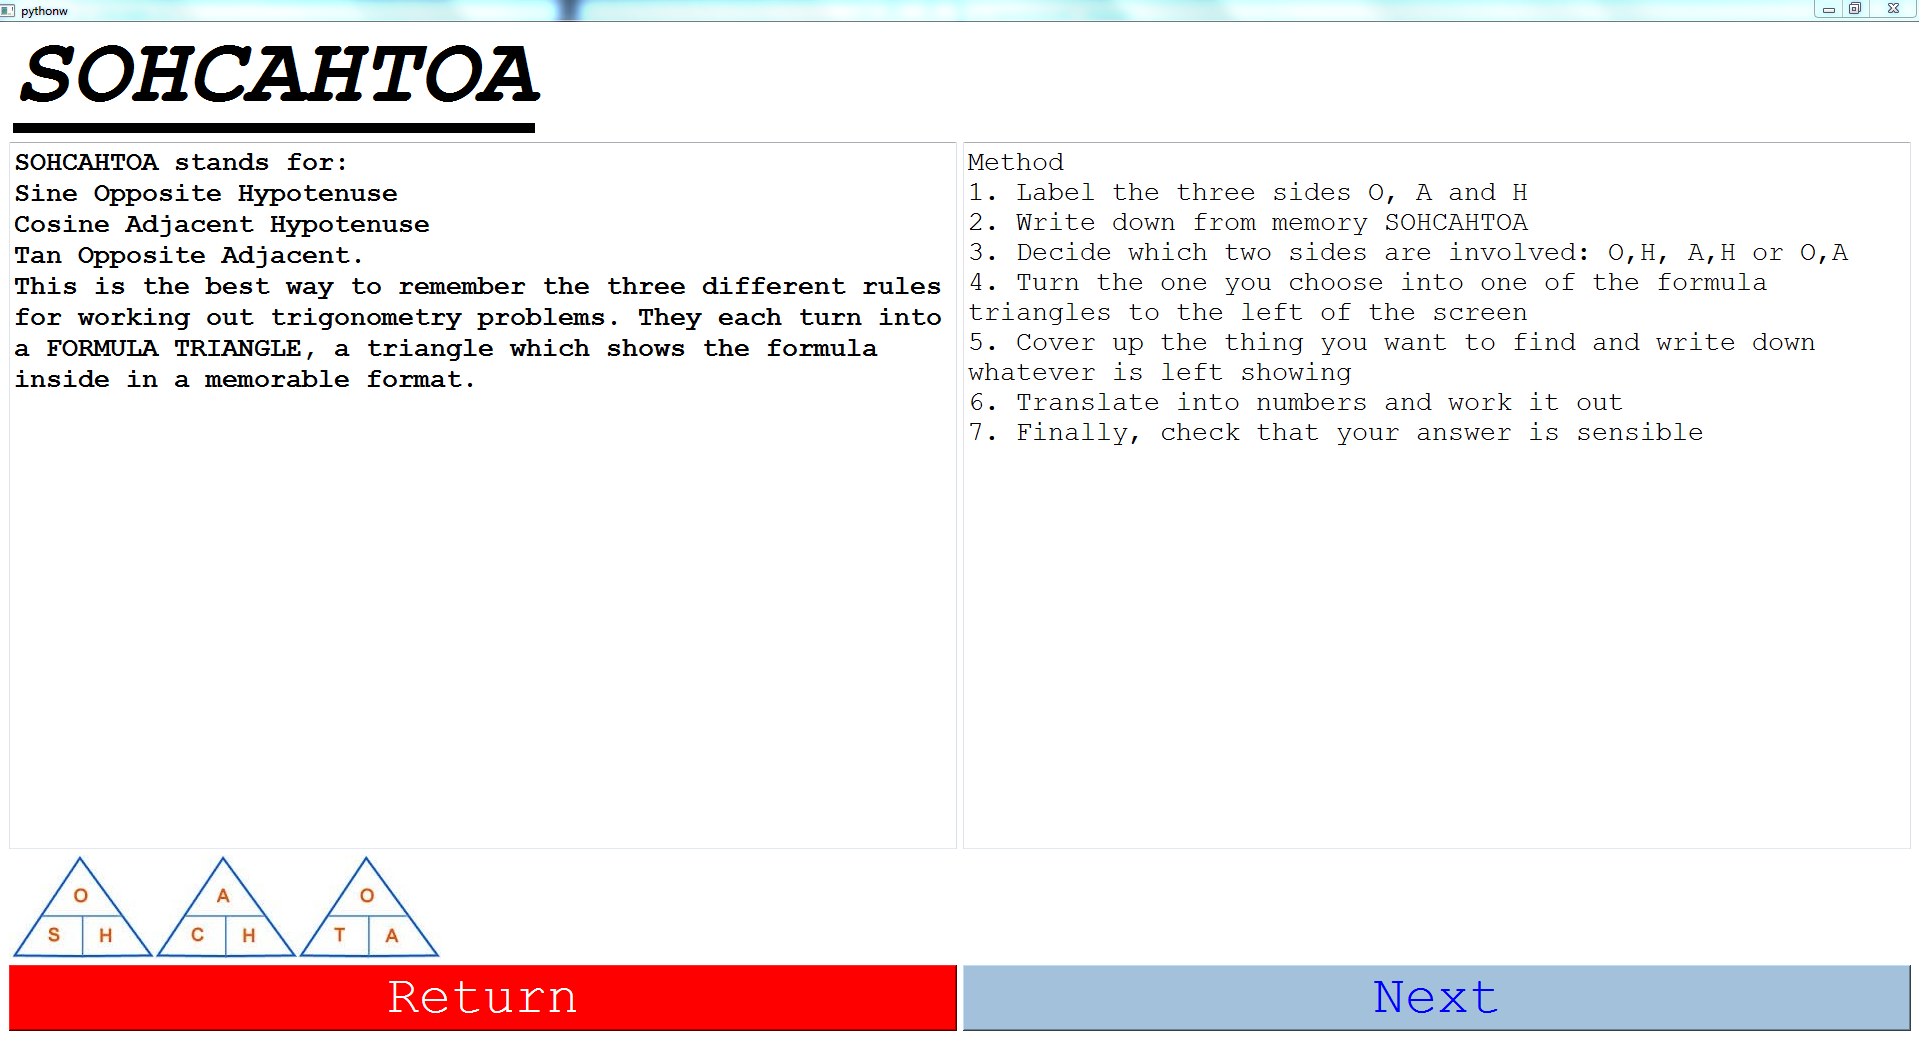
\includegraphics[width=\textwidth]{U:/git/COMP4Coursework2/Testing/screen_5}
\end{figure}

\textit{Next button is clicked: }

\begin{figure}[H]
    \label{fig: Second Screen}\caption{Second screen}
    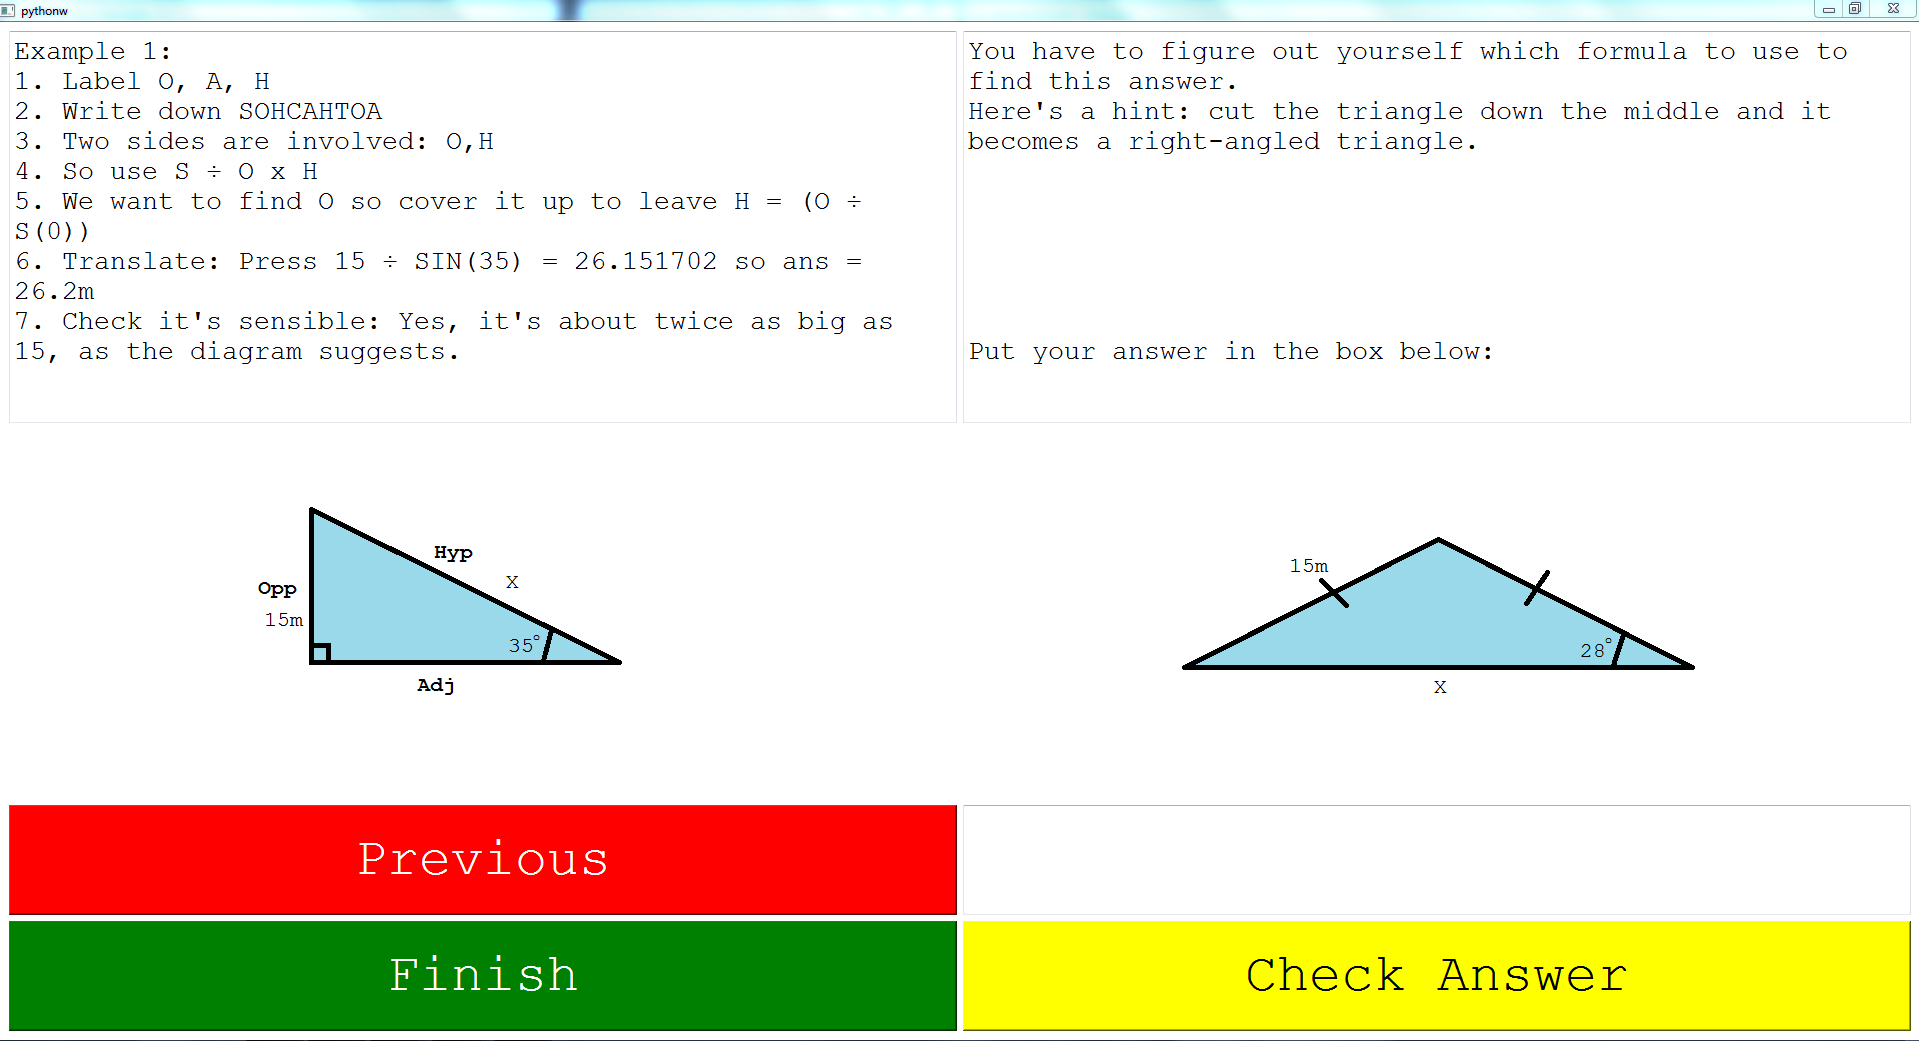
\includegraphics[width=\textwidth]{U:/git/COMP4Coursework2/Testing/screen_6}
\end{figure}

\textbf{Test 1.033}

\begin{figure}[H]
    \label{fig: First Screen}\caption{First screen}
    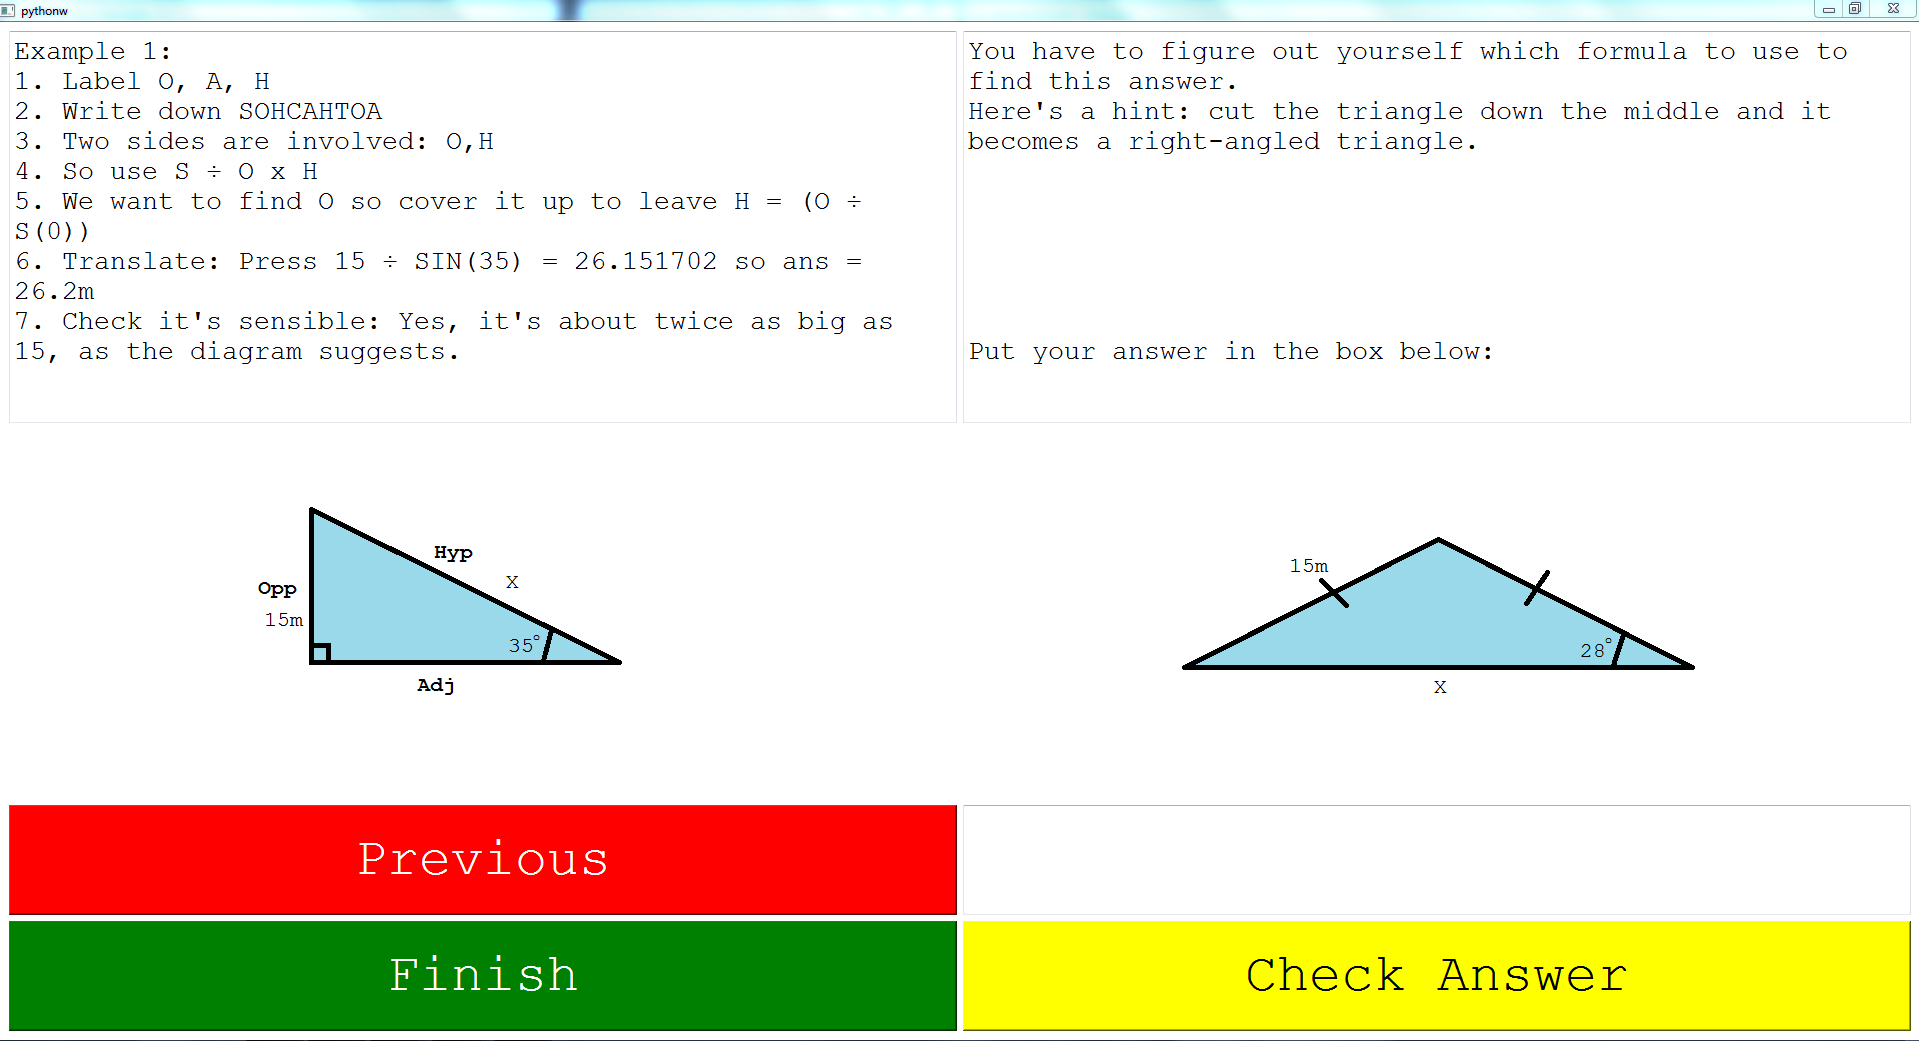
\includegraphics[width=\textwidth]{U:/git/COMP4Coursework2/Testing/screen_6}
\end{figure}

\textit{Previous button is clicked: }

\begin{figure}[H]
    \label{fig: Second Screen}\caption{Second screen}
    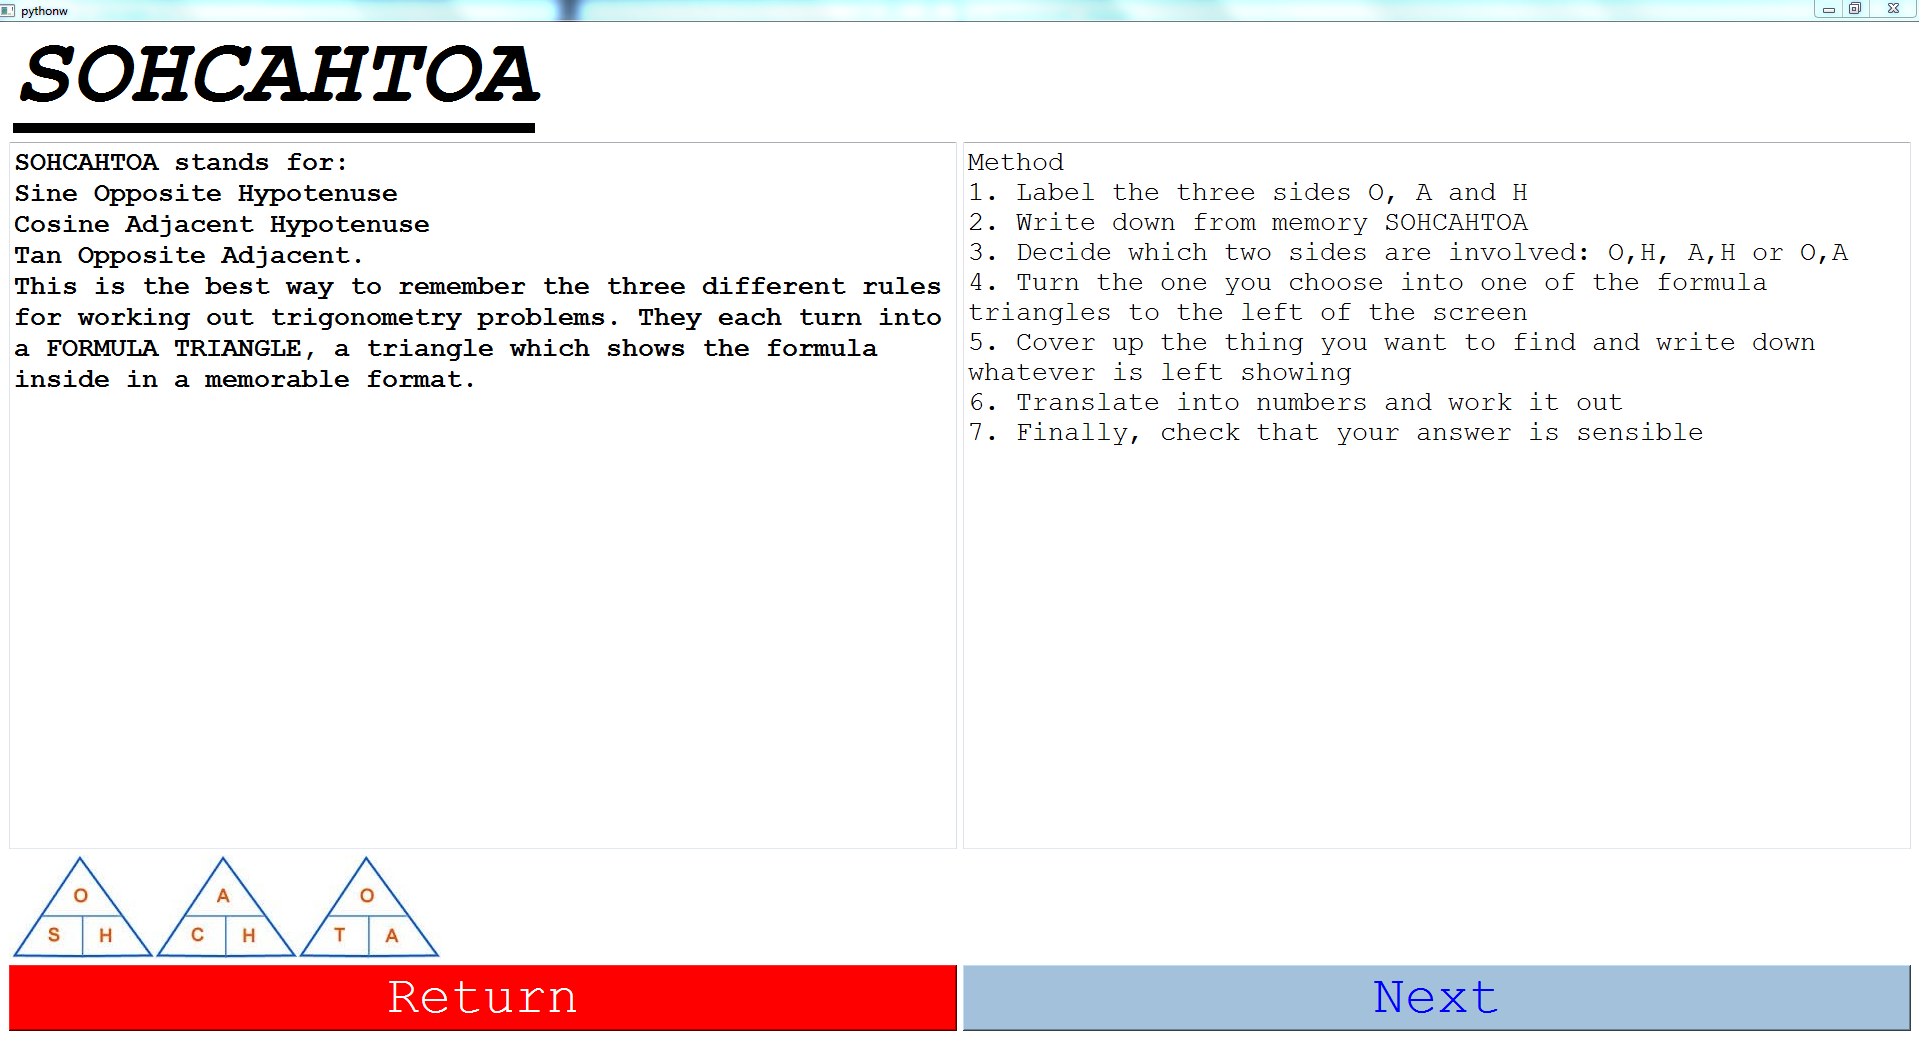
\includegraphics[width=\textwidth]{U:/git/COMP4Coursework2/Testing/screen_5}
\end{figure}

\textbf{Test 1.034}

\begin{figure}[H]
    \label{fig: First Screen}\caption{First screen}
    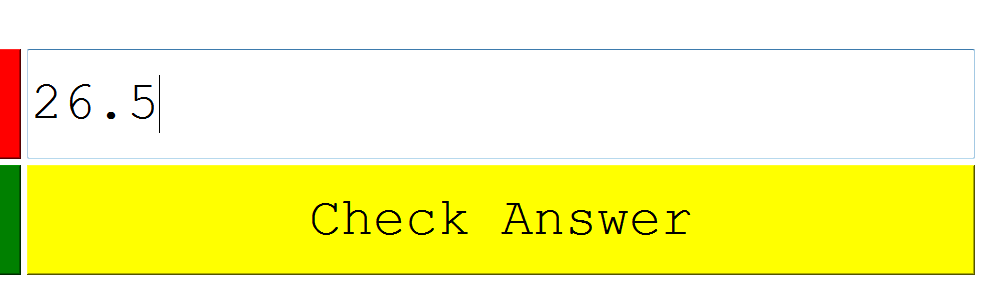
\includegraphics[width=\textwidth]{U:/git/COMP4Coursework2/Testing/screen_14}
\end{figure}

\textit{Check answer button is clicked: }

\begin{figure}[H]
    \label{fig: Second Screen}\caption{Second screen}
    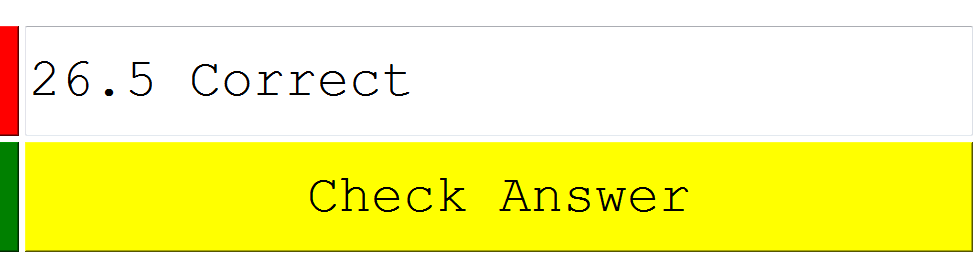
\includegraphics[width=\textwidth]{U:/git/COMP4Coursework2/Testing/screen_15}
\end{figure}

\textbf{Test 1.035}

\begin{figure}[H]
    \label{fig: First Screen}\caption{First screen}
    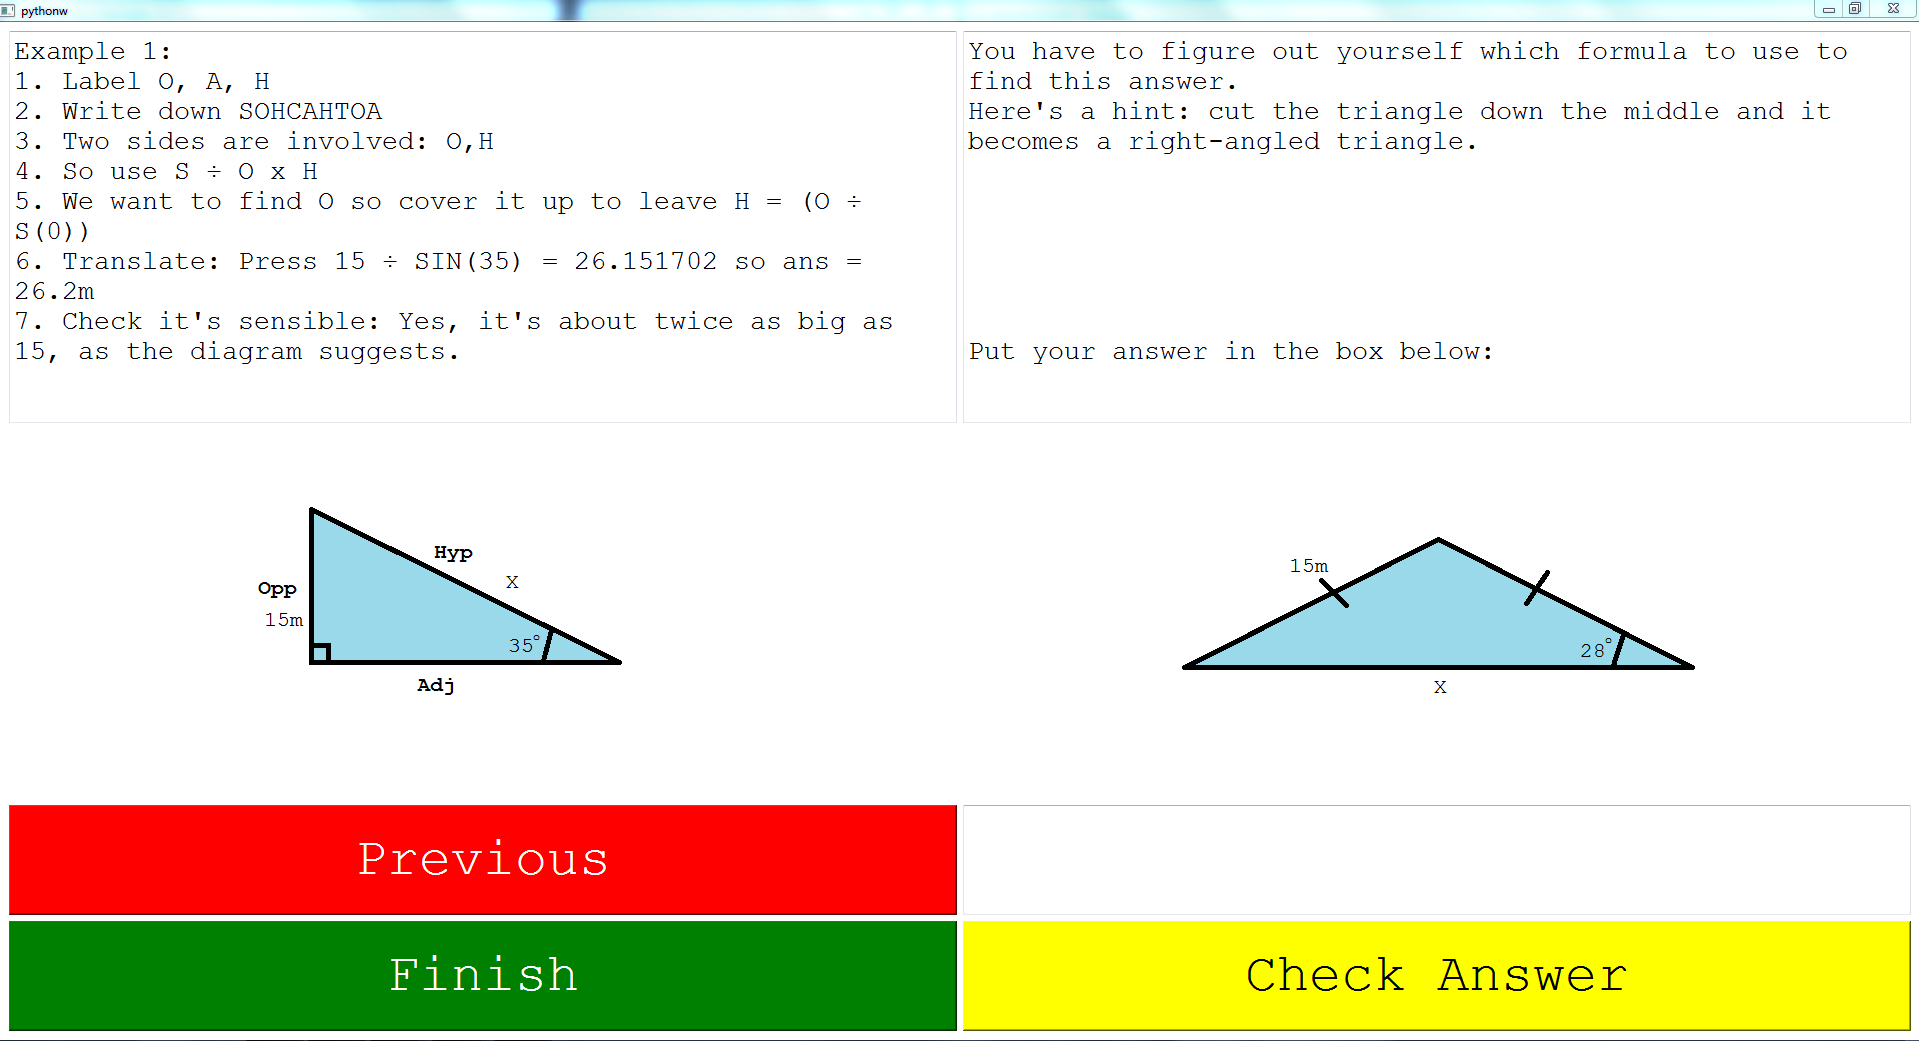
\includegraphics[width=\textwidth]{U:/git/COMP4Coursework2/Testing/screen_6}
\end{figure}

\textit{Finish button is clicked: }

\begin{figure}[H]
    \label{fig: Second Screen}\caption{Second screen}
    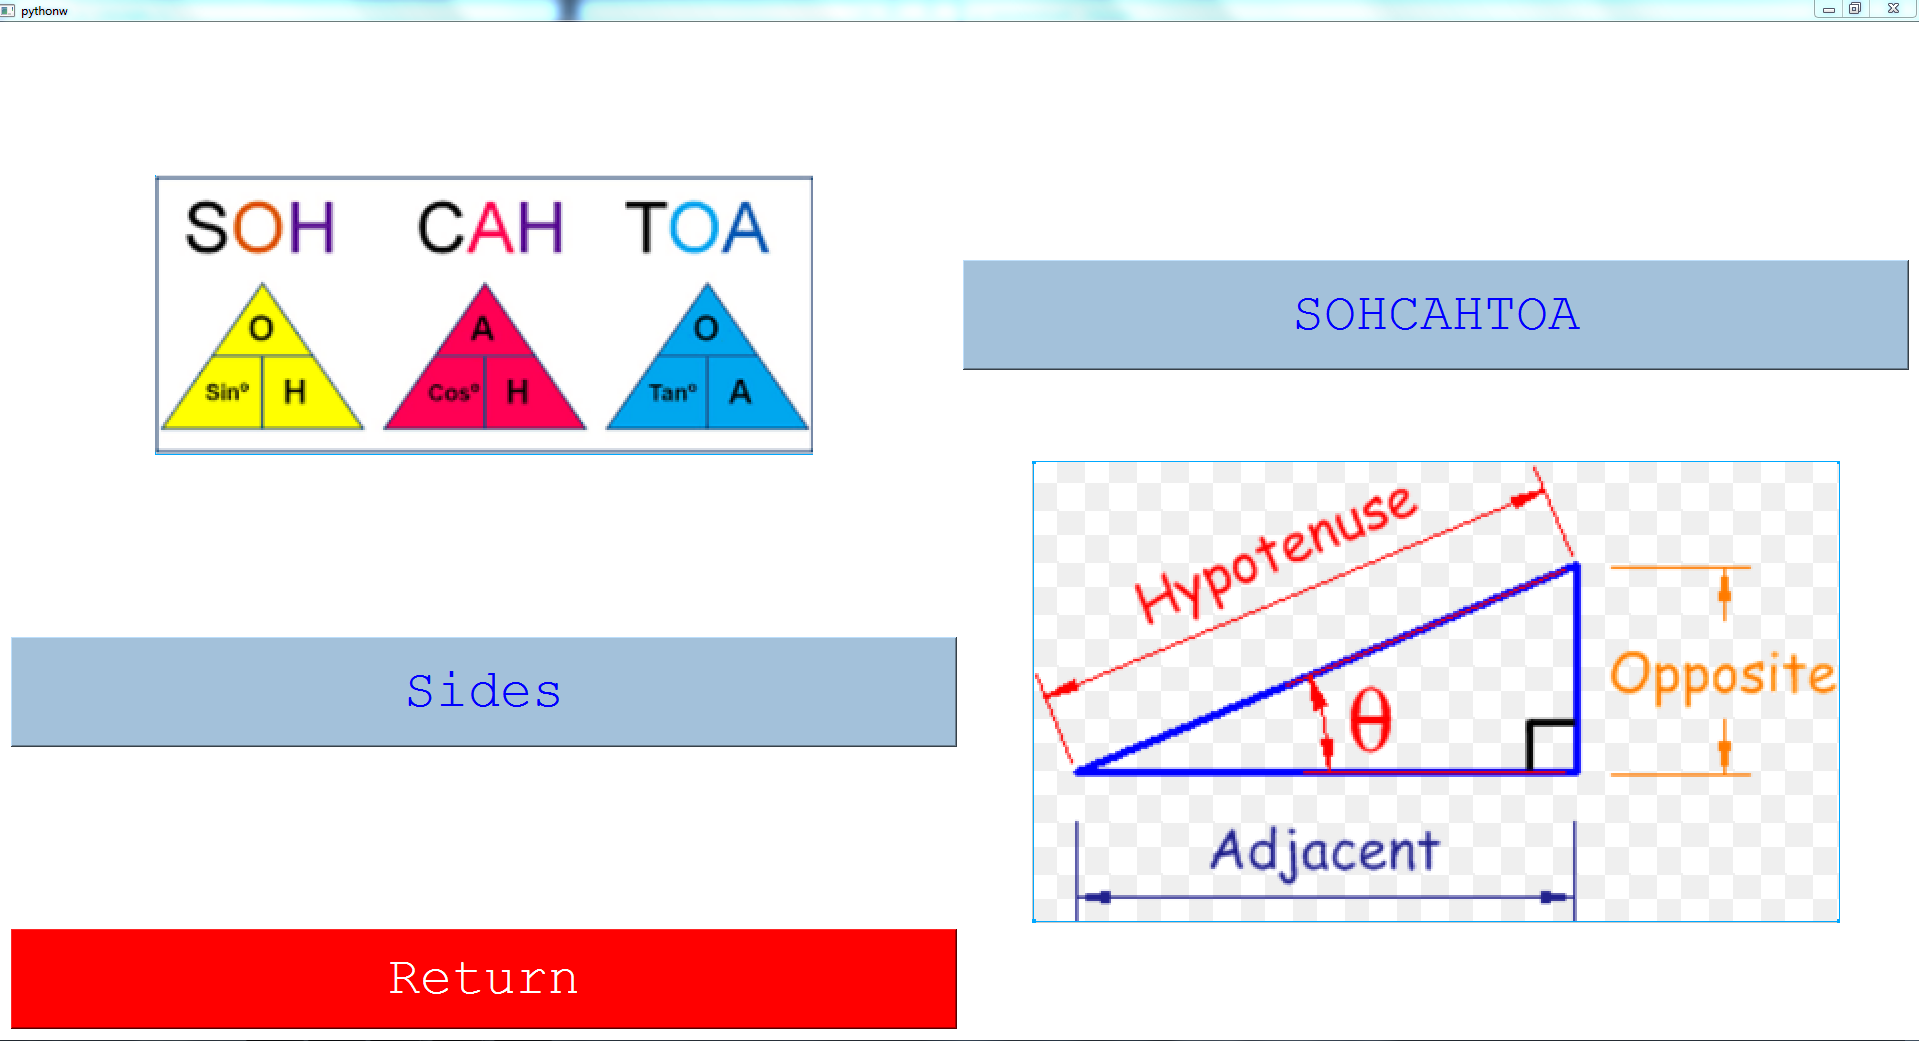
\includegraphics[width=\textwidth]{U:/git/COMP4Coursework2/Testing/screen_4}
\end{figure}

\textbf{Test 1.097}

\begin{figure}[H]
    \label{fig: First Screen}\caption{First screen}
    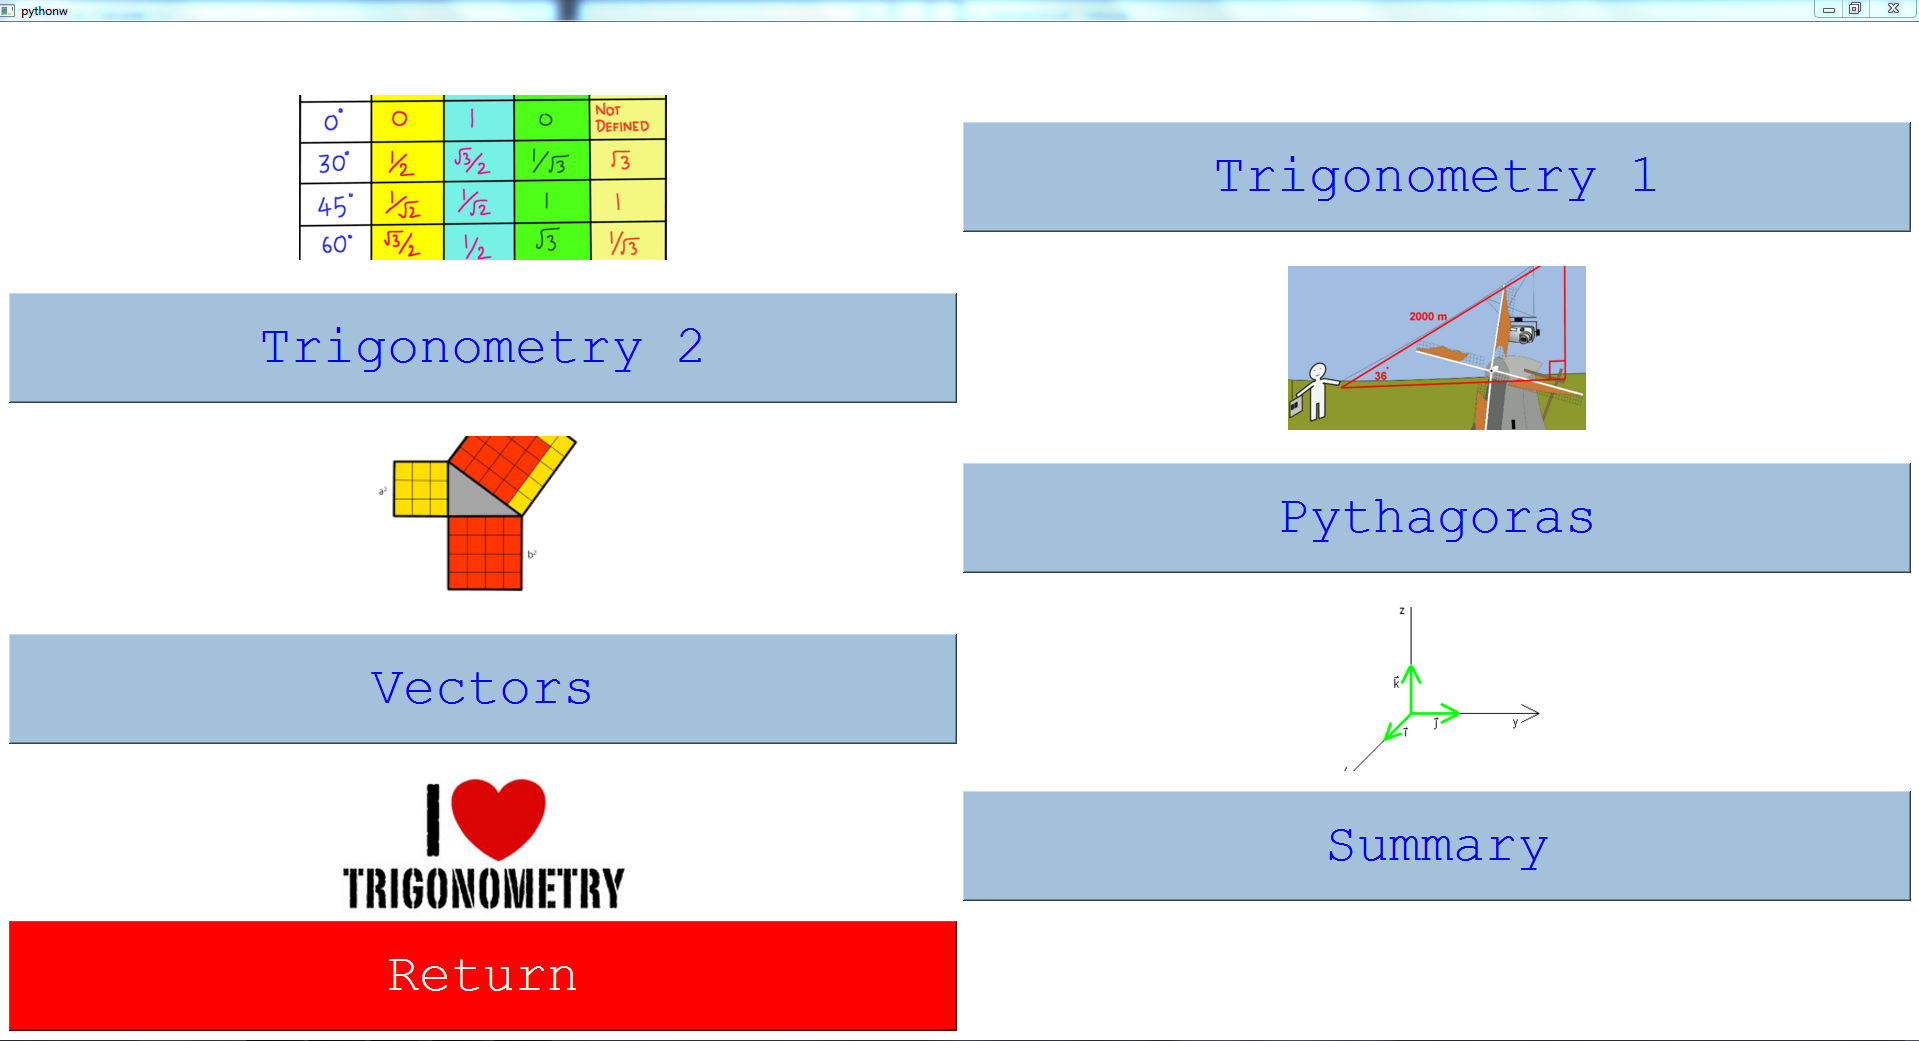
\includegraphics[width=\textwidth]{U:/git/COMP4Coursework2/Testing/screen_7}
\end{figure}

\textit{Trigonometry 1 button is clicked: }

\begin{figure}[H]
    \label{fig: Second Screen}\caption{Second screen}
    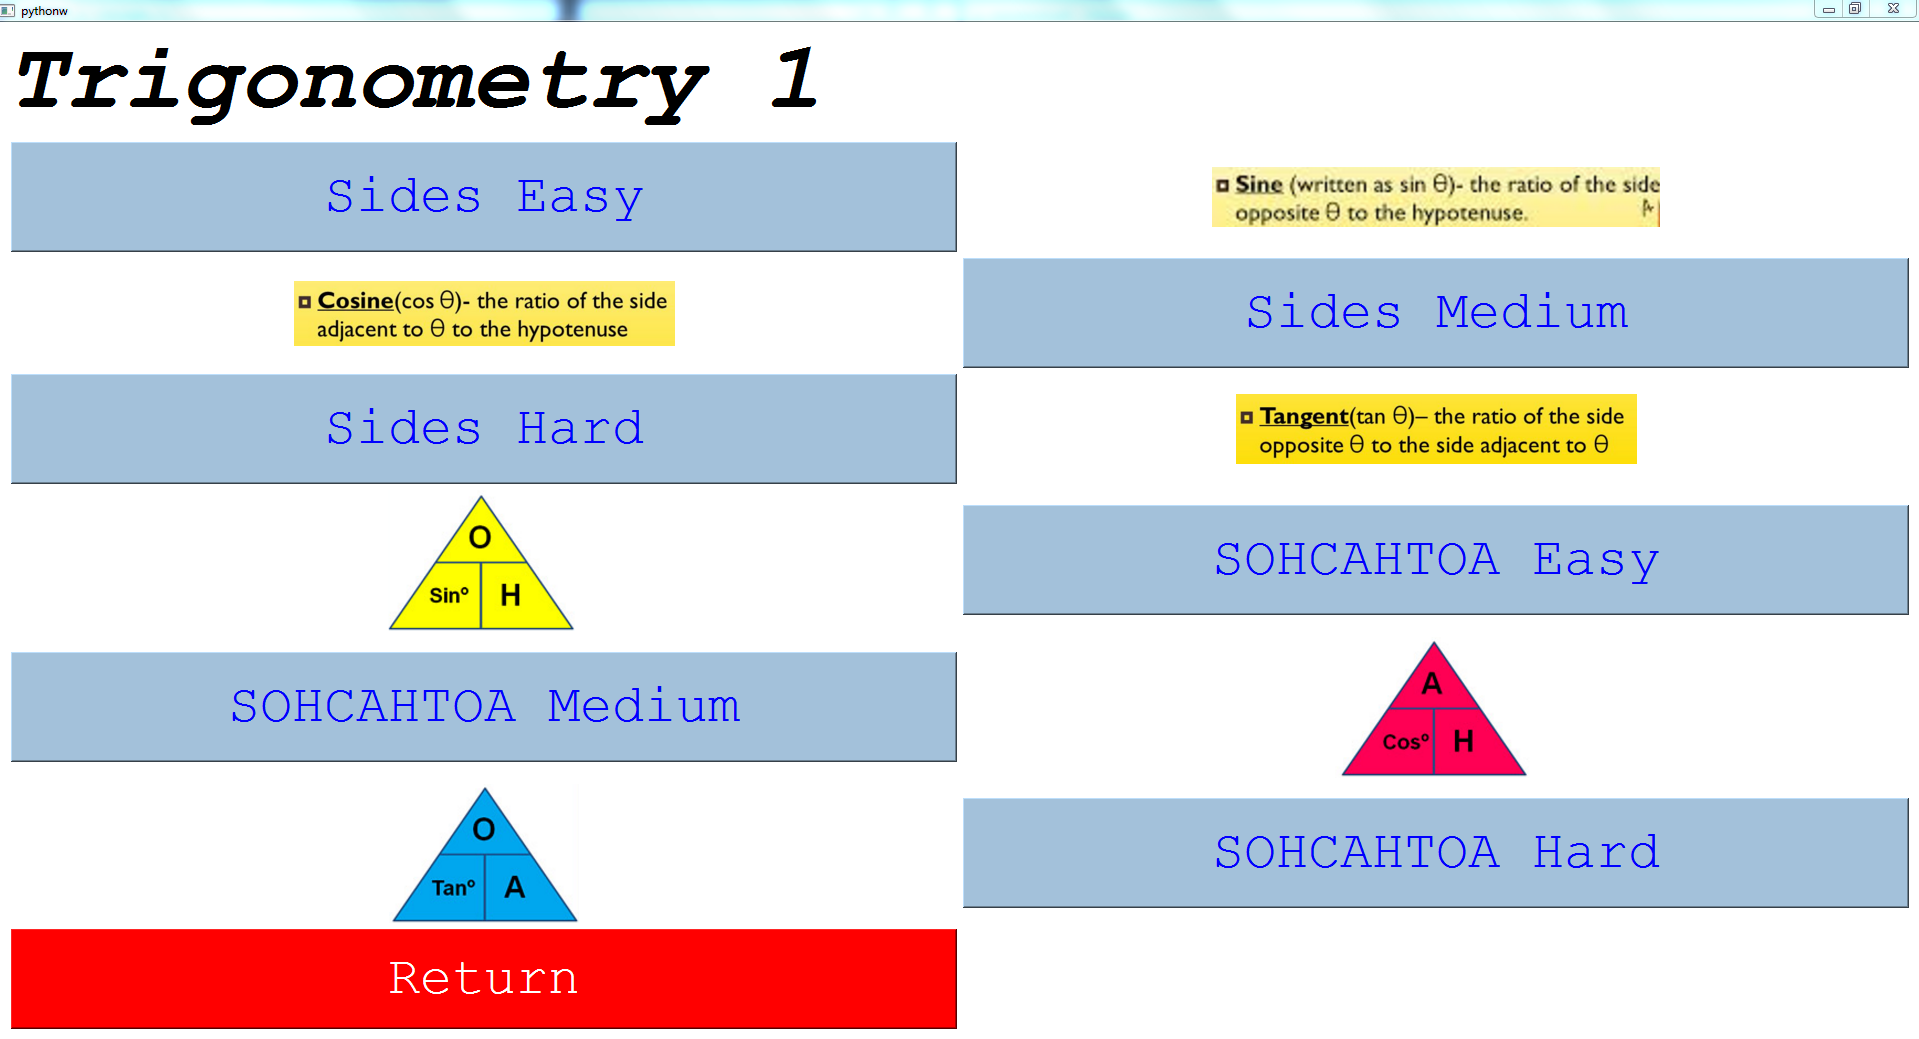
\includegraphics[width=\textwidth]{U:/git/COMP4Coursework2/Testing/screen_8}
\end{figure}

\textbf{Test 1.102}

\begin{figure}[H]
    \label{fig: First Screen}\caption{First screen}
    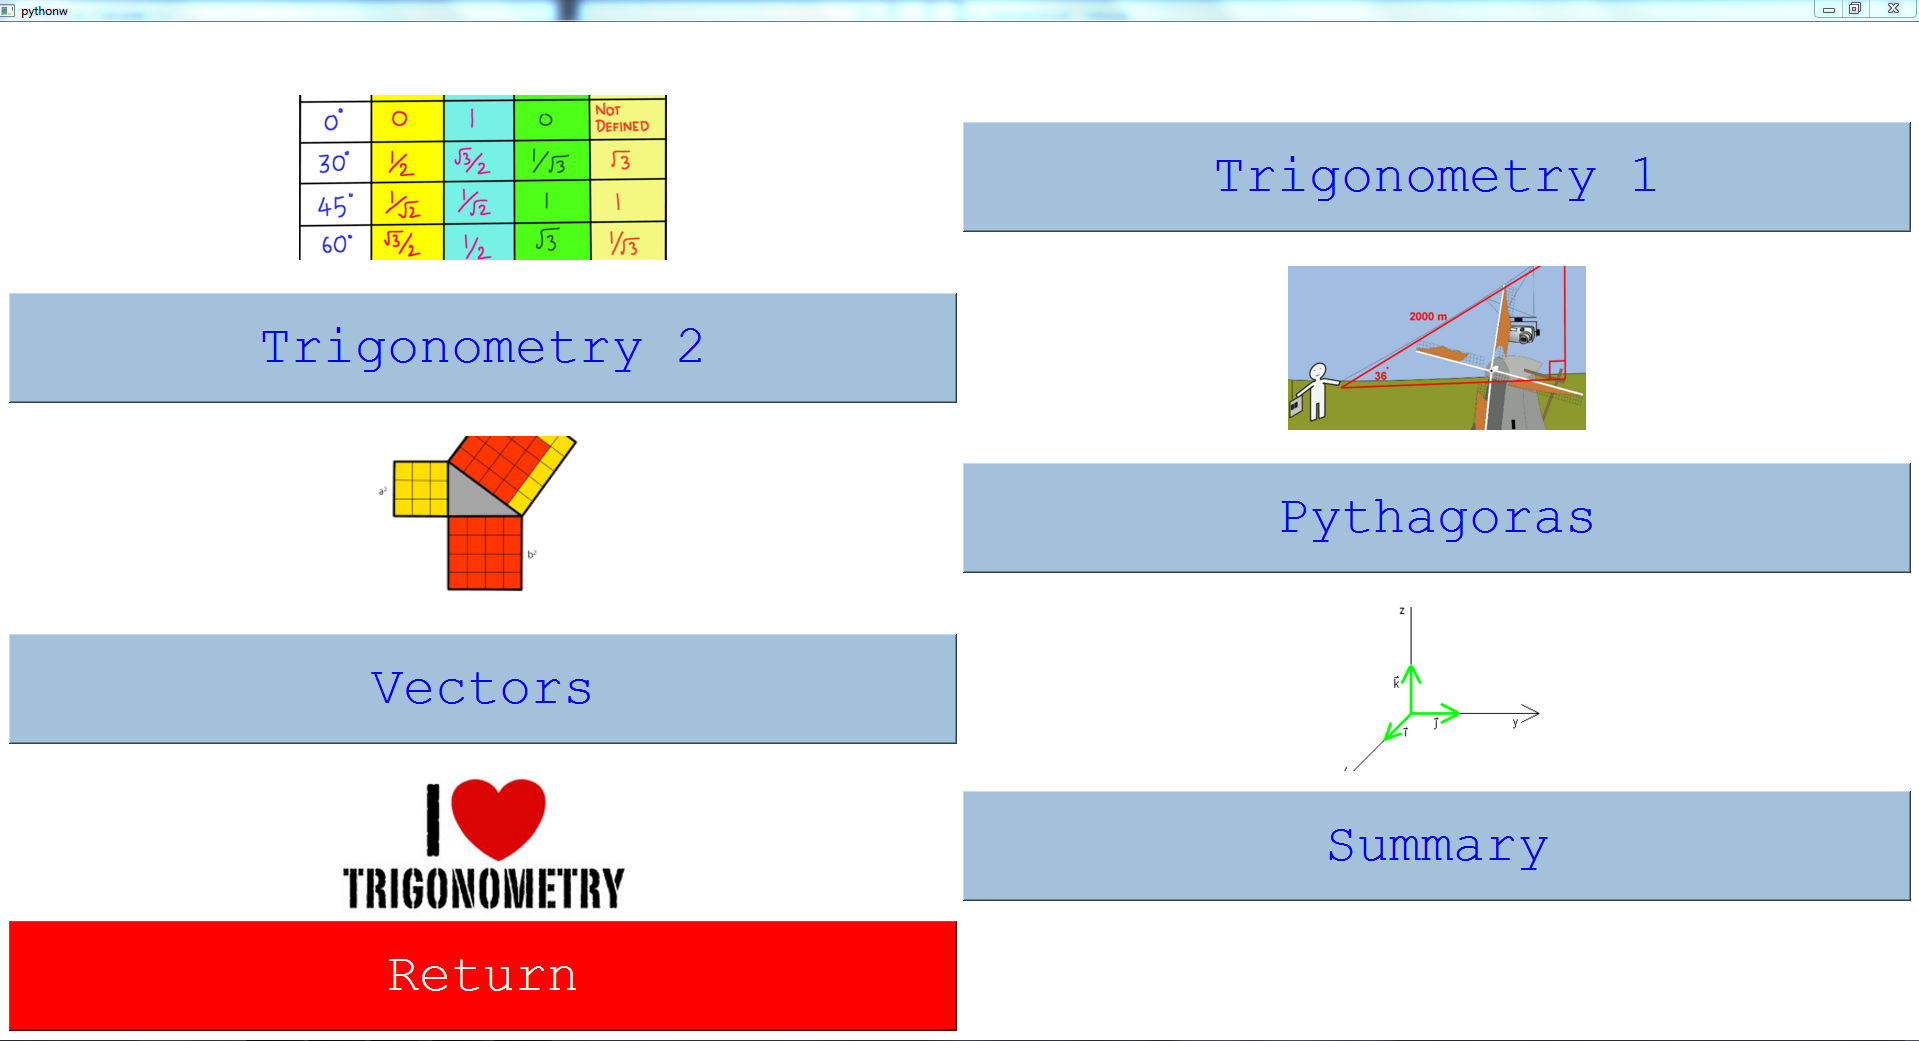
\includegraphics[width=\textwidth]{U:/git/COMP4Coursework2/Testing/screen_7}
\end{figure}

\textit{Return button is clicked: }

\begin{figure}[H]
    \label{fig: Second Screen}\caption{Second screen}
    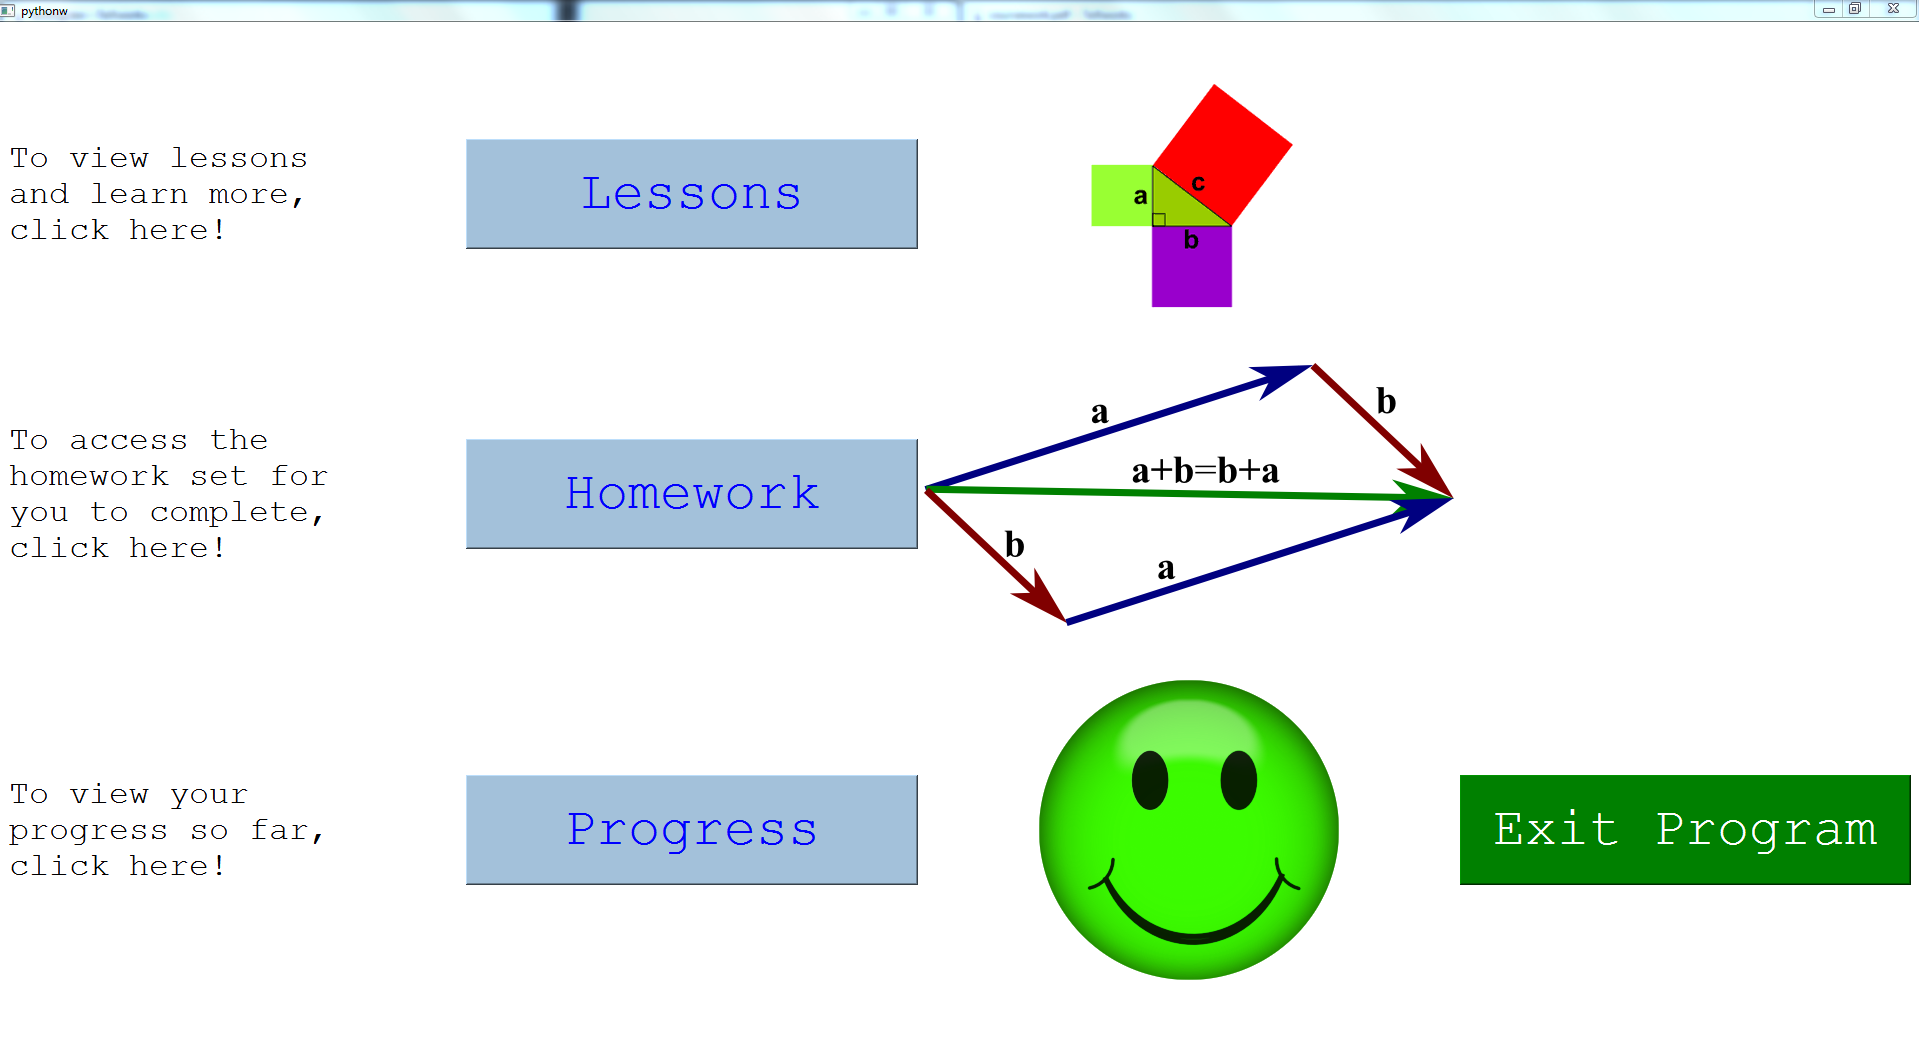
\includegraphics[width=\textwidth]{U:/git/COMP4Coursework2/Testing/screen_2}
\end{figure}

\textbf{Test 1.103}

\begin{figure}[H]
    \label{fig: First Screen}\caption{First screen}
    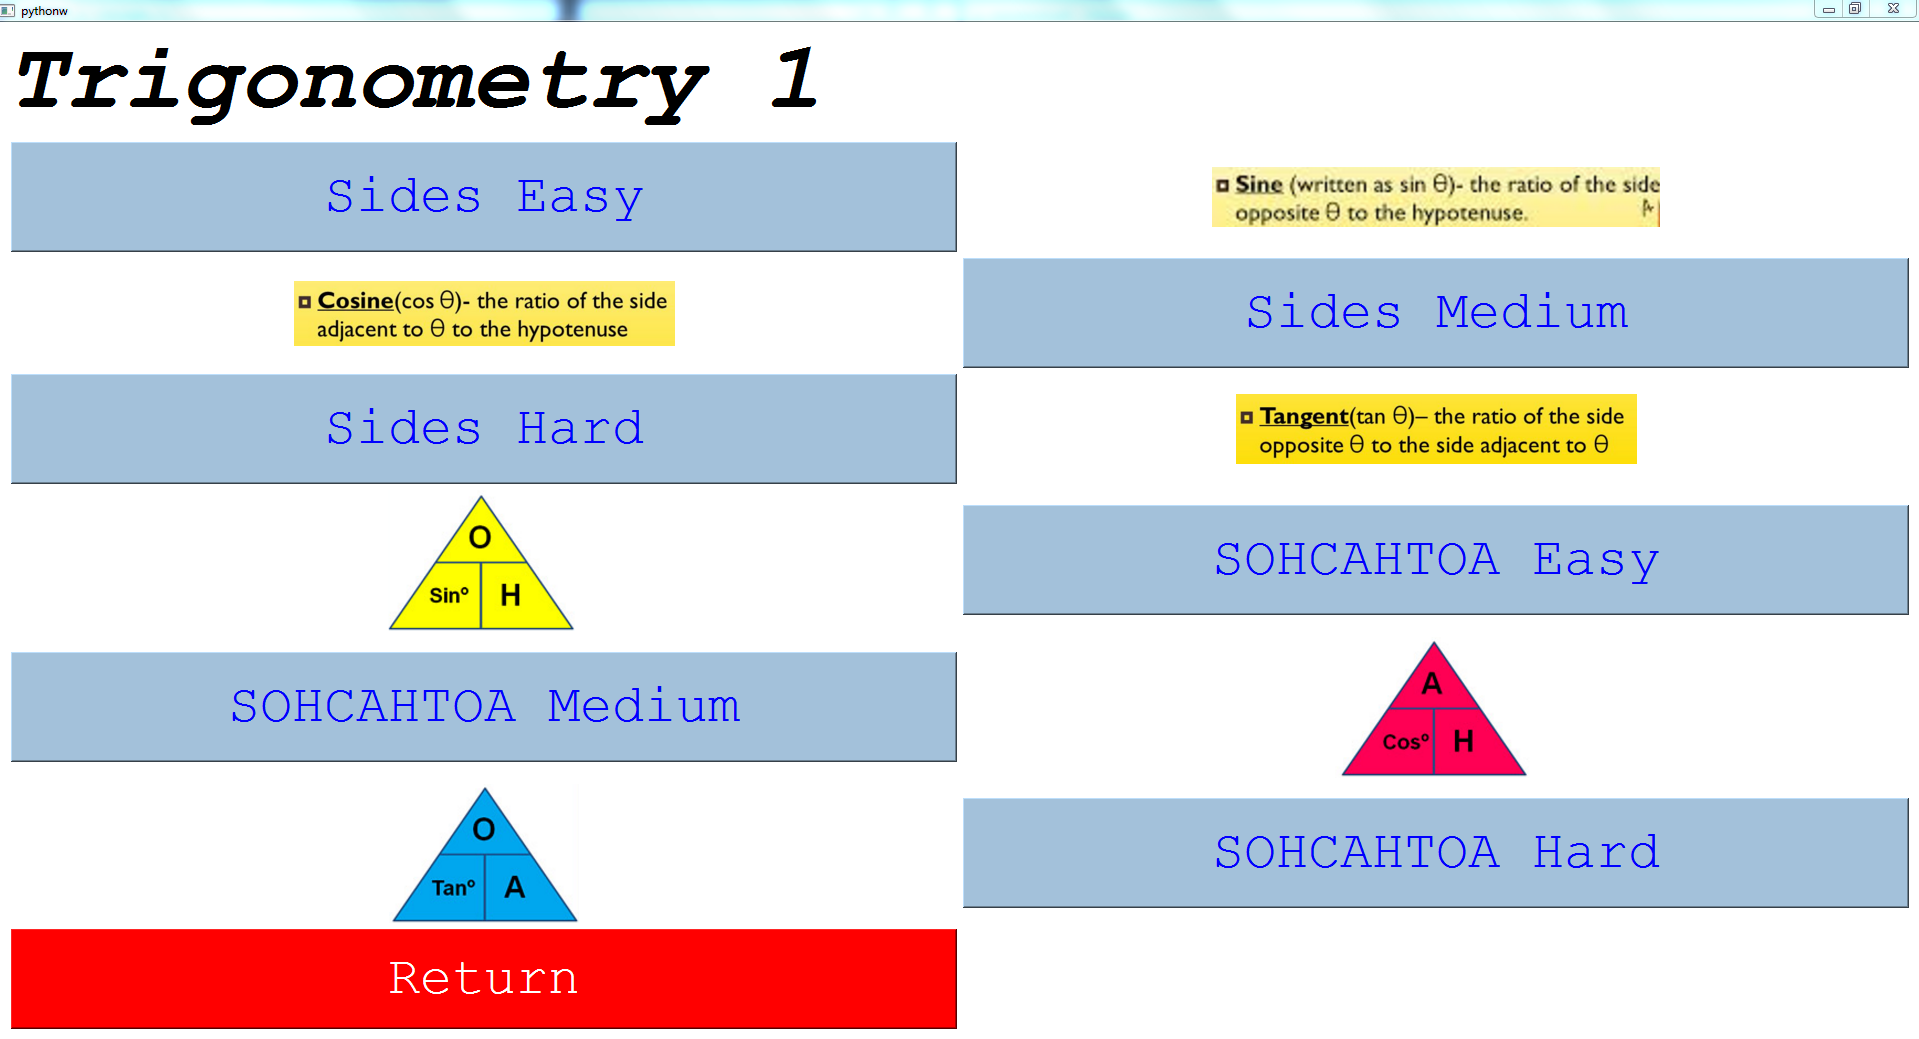
\includegraphics[width=\textwidth]{U:/git/COMP4Coursework2/Testing/screen_8}
\end{figure}

\textit{Sides easy button is clicked: }

\begin{figure}[H]
    \label{fig: Second Screen}\caption{Second screen}
    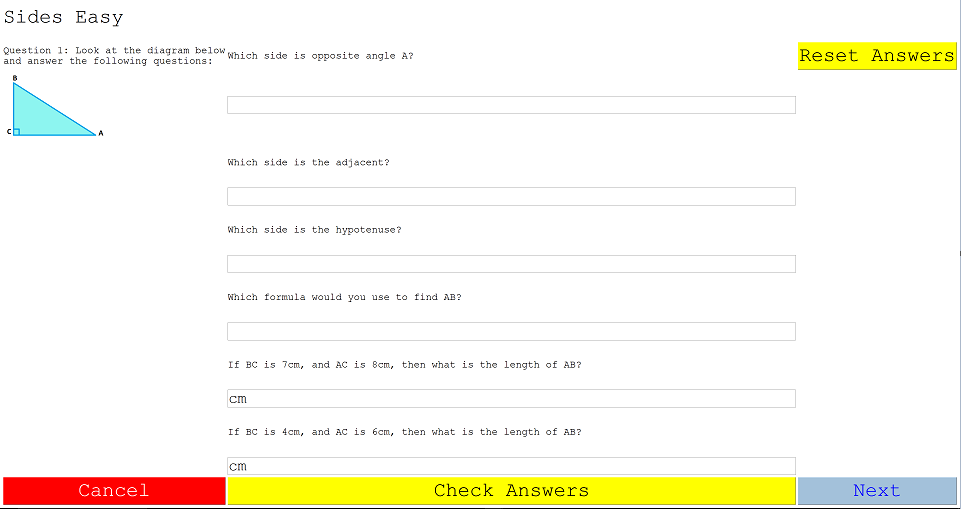
\includegraphics[width=\textwidth]{U:/git/COMP4Coursework2/Testing/screen_9}
\end{figure}

\textbf{Test 1.135}

\begin{figure}[H]
    \label{fig: First Screen}\caption{First screen}
    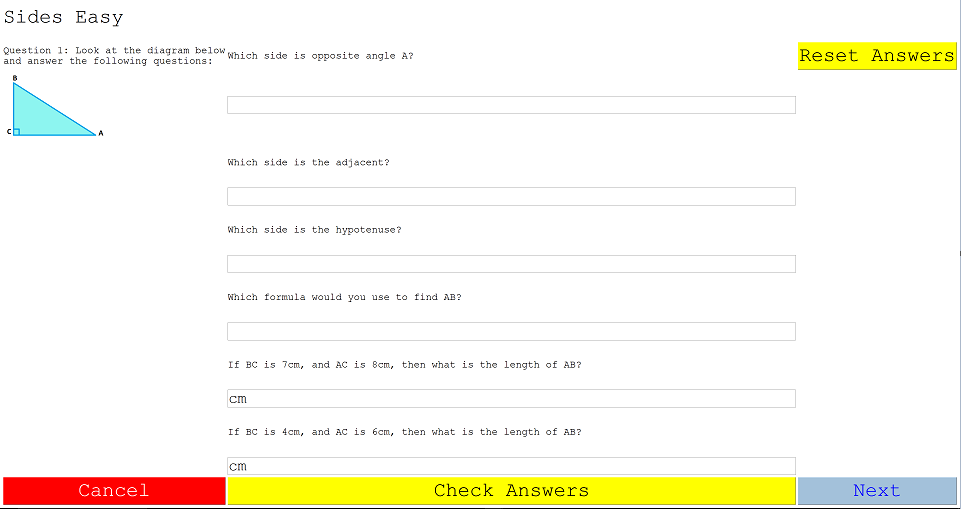
\includegraphics[width=\textwidth]{U:/git/COMP4Coursework2/Testing/screen_9}
\end{figure}

\textit{Return button is clicked: }

\begin{figure}[H]
    \label{fig: Second Screen}\caption{Second screen}
    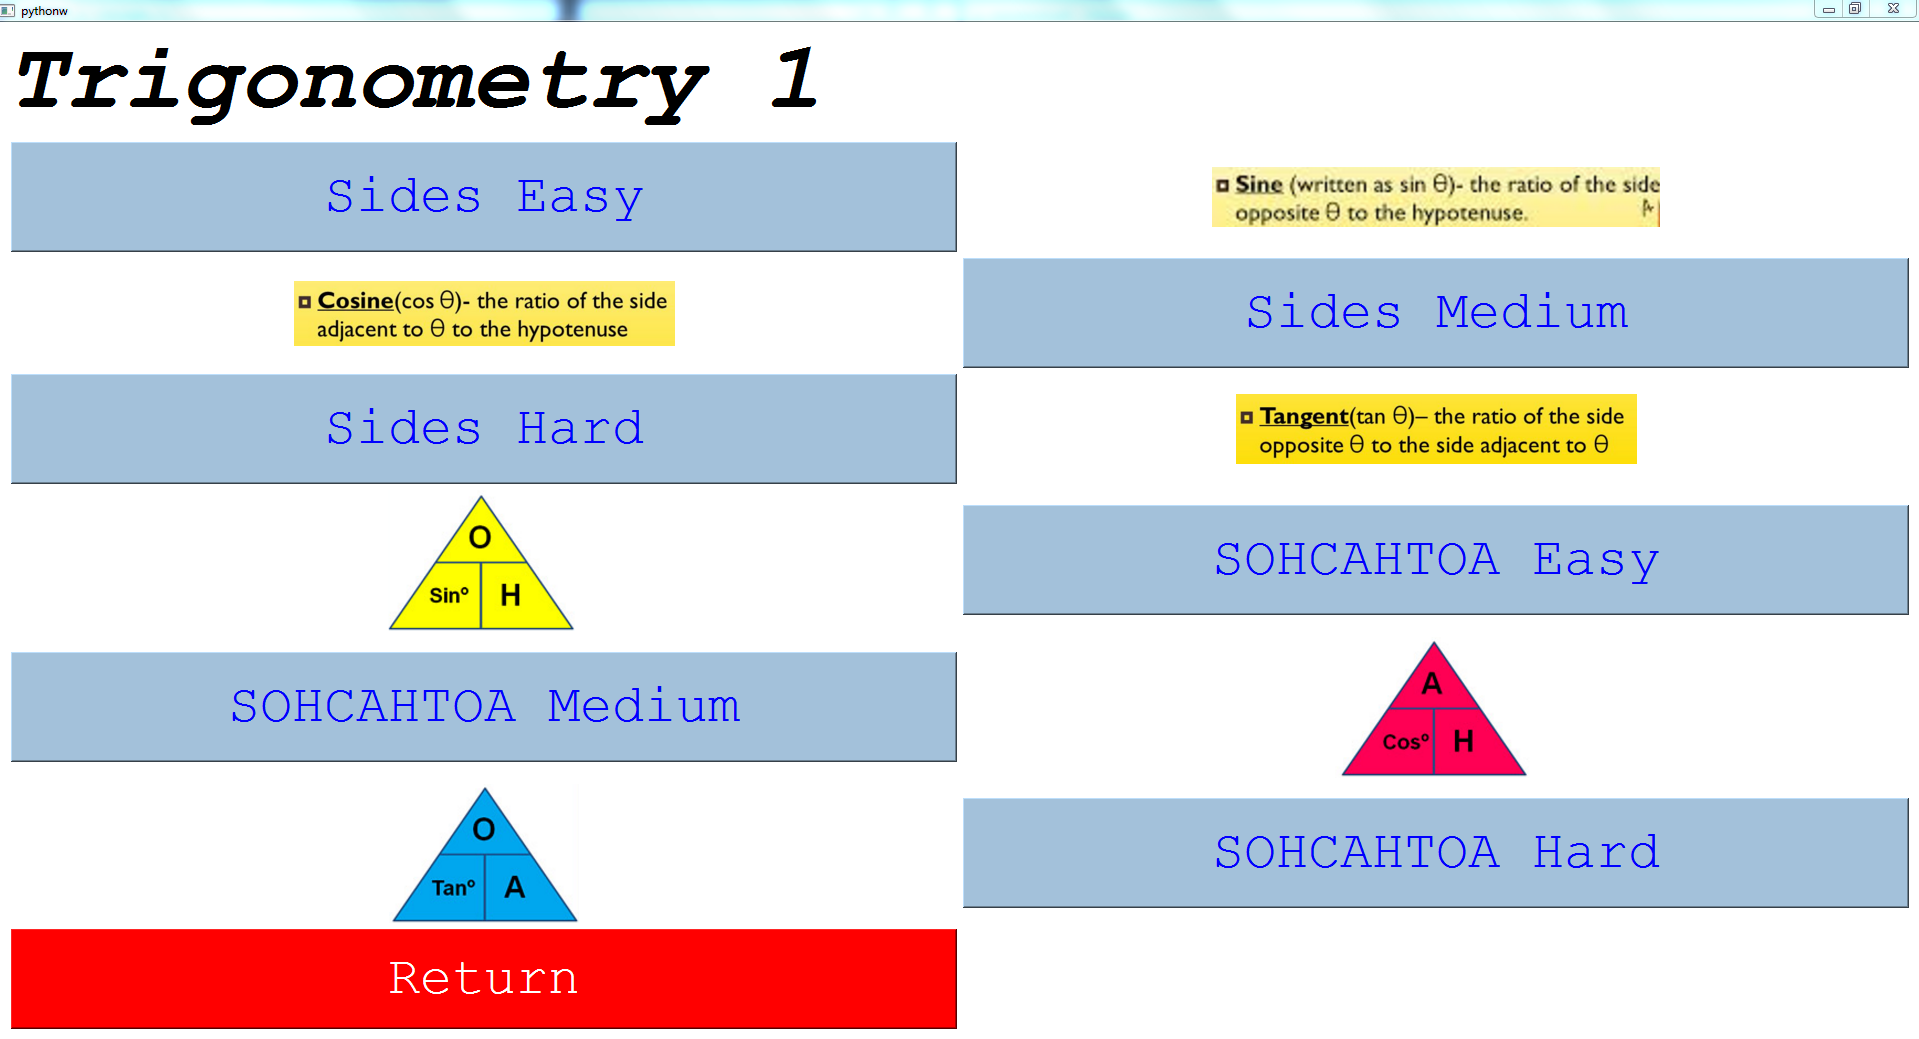
\includegraphics[width=\textwidth]{U:/git/COMP4Coursework2/Testing/screen_8}
\end{figure}

\textbf{Test 1.136}

\begin{figure}[H]
    \label{fig: First Screen}\caption{First screen}
    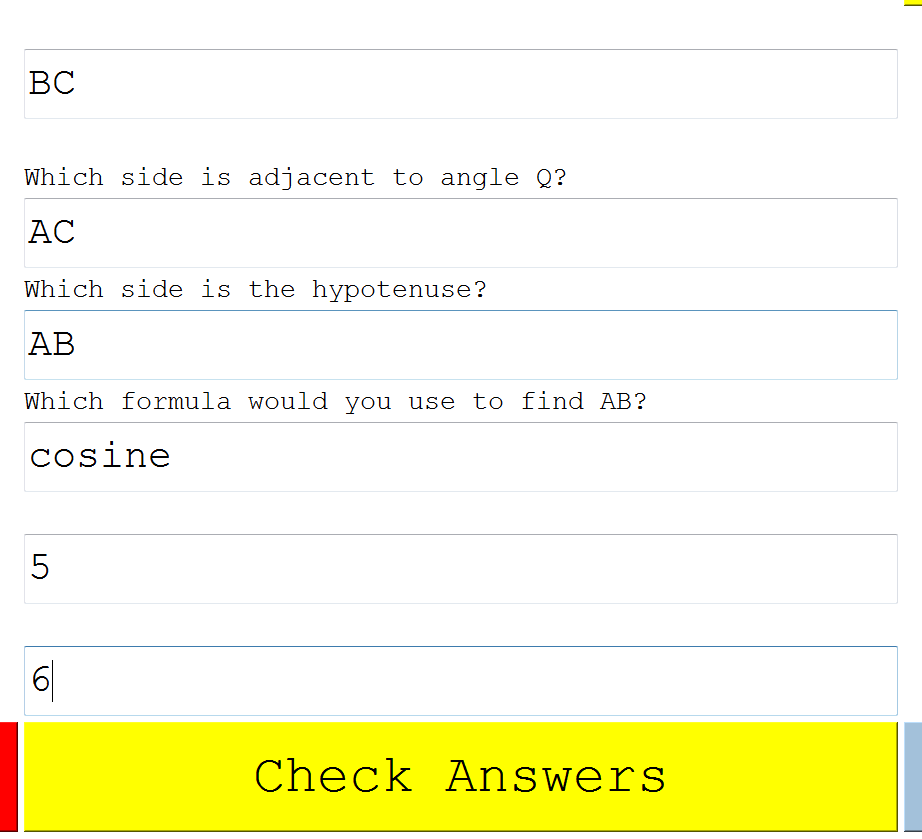
\includegraphics[width=\textwidth]{U:/git/COMP4Coursework2/Testing/screen_16}
\end{figure}

\textit{Check answers button is clicked: }

\begin{figure}[H]
    \label{fig: Second Screen}\caption{Second screen}
    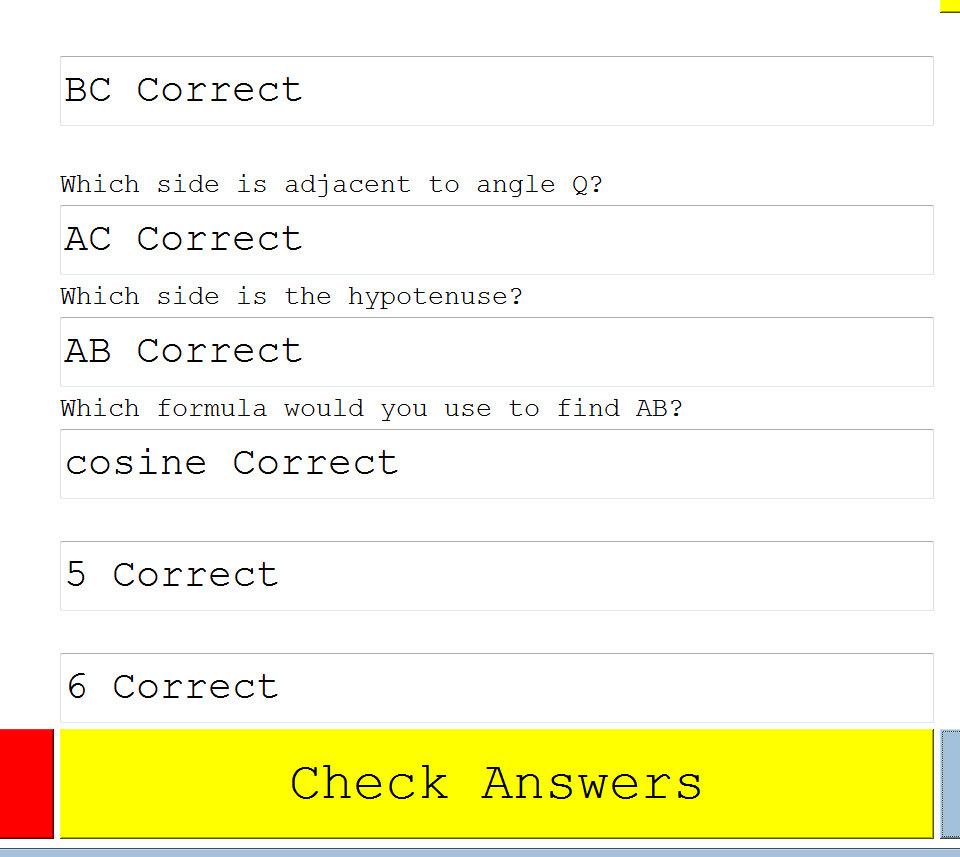
\includegraphics[width=\textwidth]{U:/git/COMP4Coursework2/Testing/screen_17}
\end{figure}

\textbf{Test 1.137}

\begin{figure}[H]
    \label{fig: First Screen}\caption{First screen}
    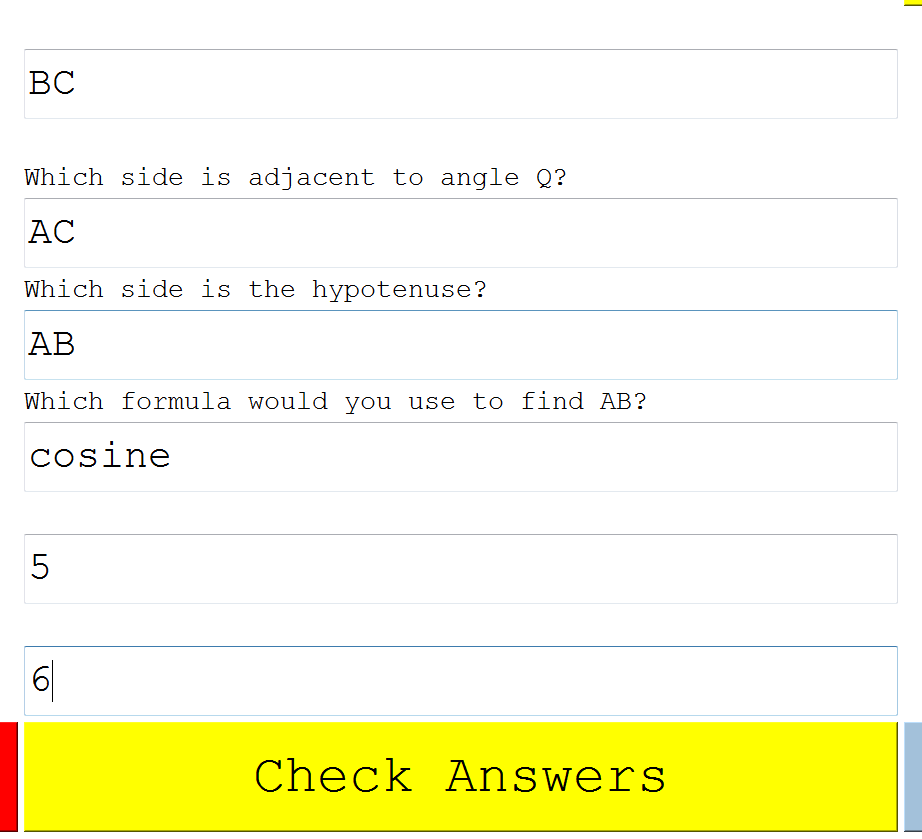
\includegraphics[width=\textwidth]{U:/git/COMP4Coursework2/Testing/screen_16}
\end{figure}

\textit{Reset answers button is clicked: }

\begin{figure}[H]
    \label{fig: Second Screen}\caption{Second screen}
    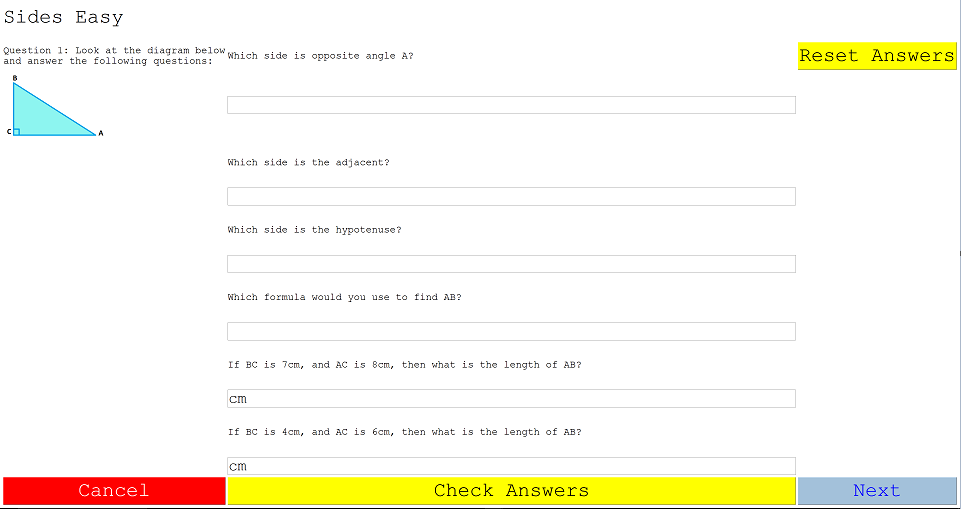
\includegraphics[width=\textwidth]{U:/git/COMP4Coursework2/Testing/screen_9}
\end{figure}

\textbf{Test 1.138}

\begin{figure}[H]
    \label{fig: First Screen}\caption{First screen}
    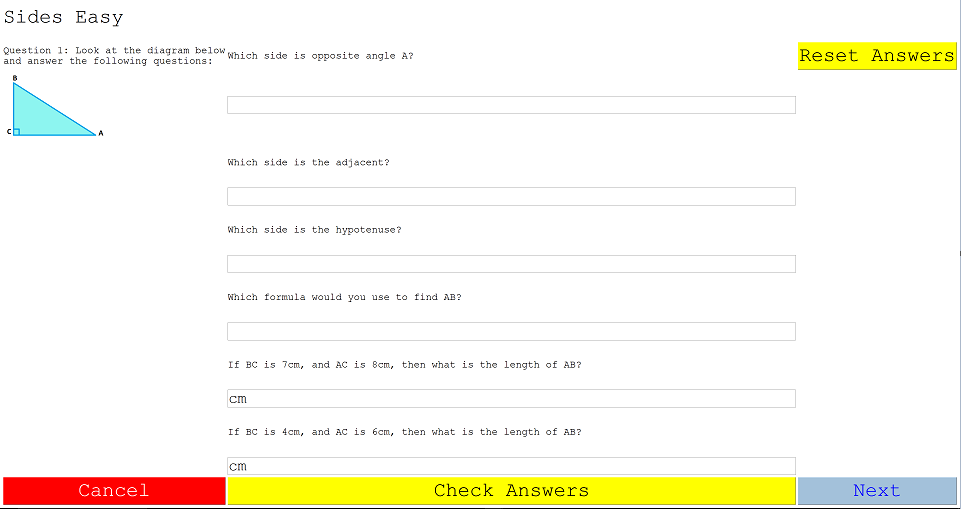
\includegraphics[width=\textwidth]{U:/git/COMP4Coursework2/Testing/screen_9}
\end{figure}

\textit{Next button is clicked: }

\begin{figure}[H]
    \label{fig: Second Screen}\caption{Second screen}
    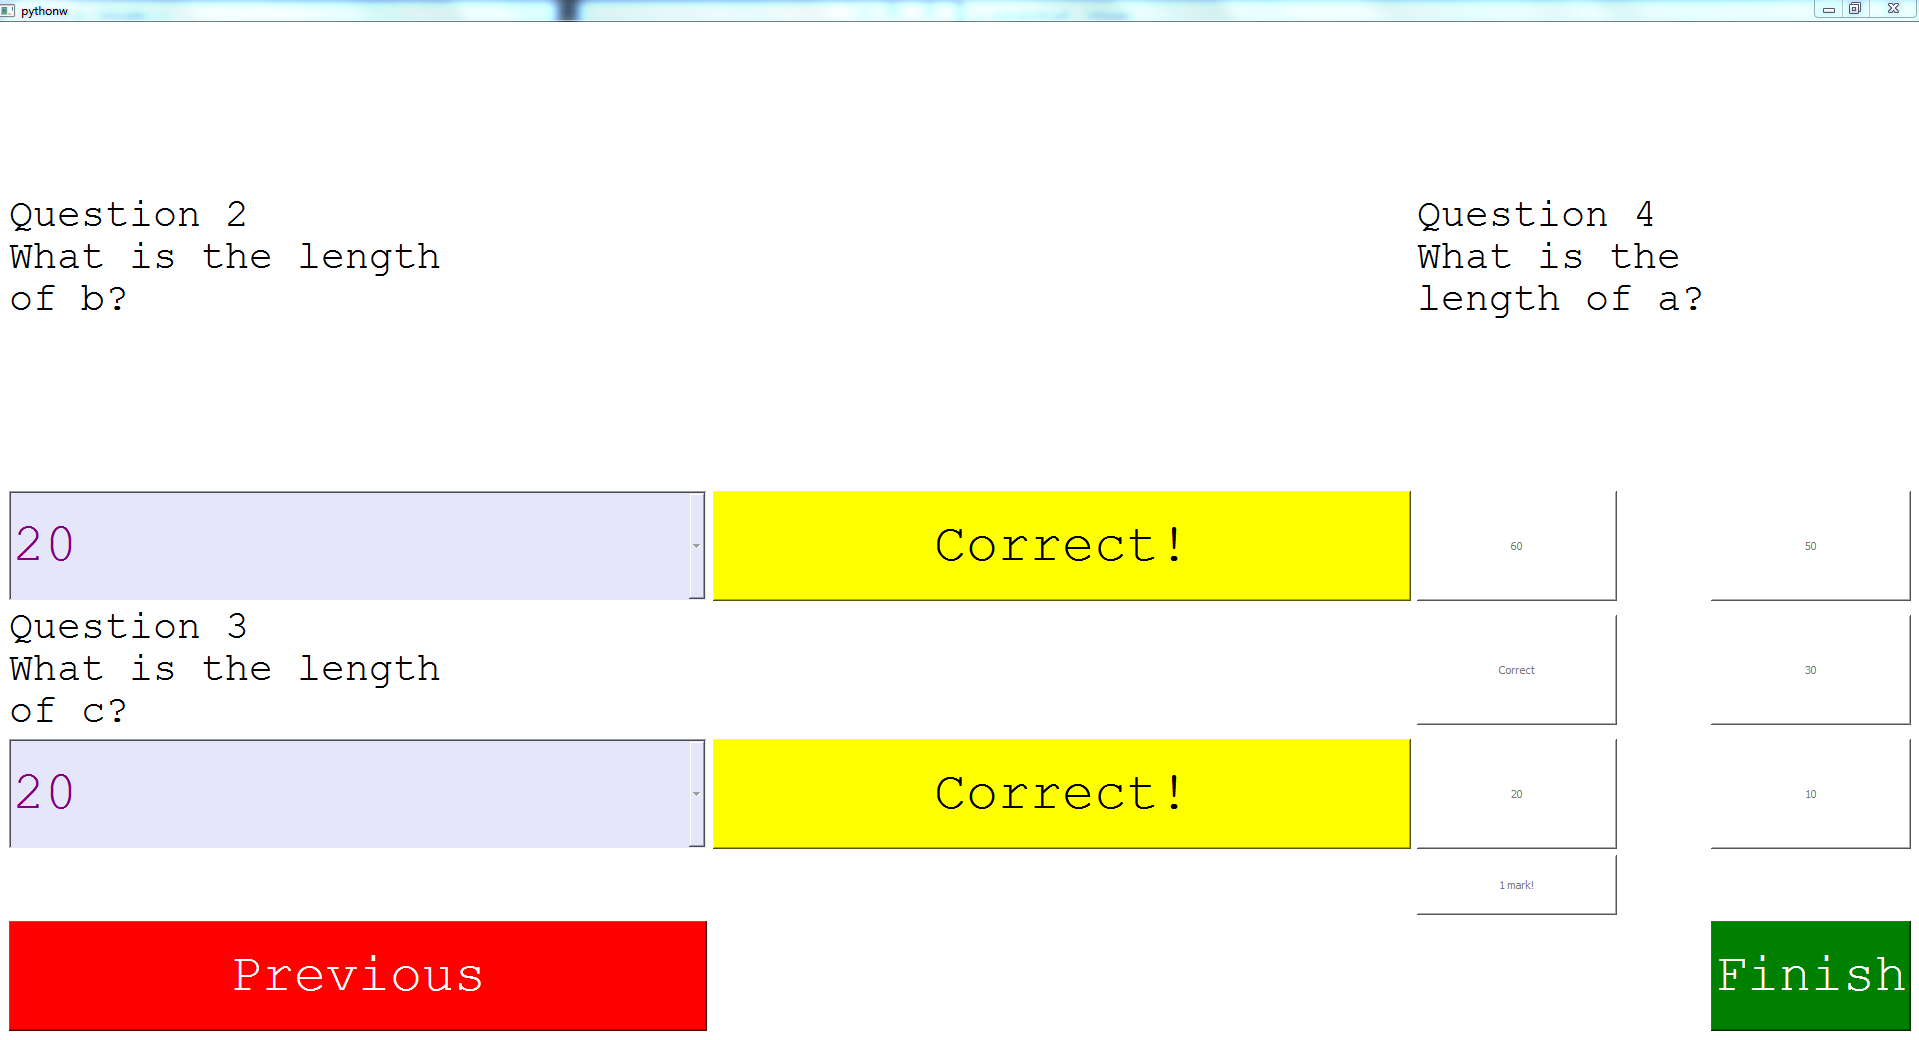
\includegraphics[width=\textwidth]{U:/git/COMP4Coursework2/Testing/screen_10}
\end{figure}

\textbf{Test 1.139}

\begin{figure}[H]
    \label{fig: First Screen}\caption{First screen}
    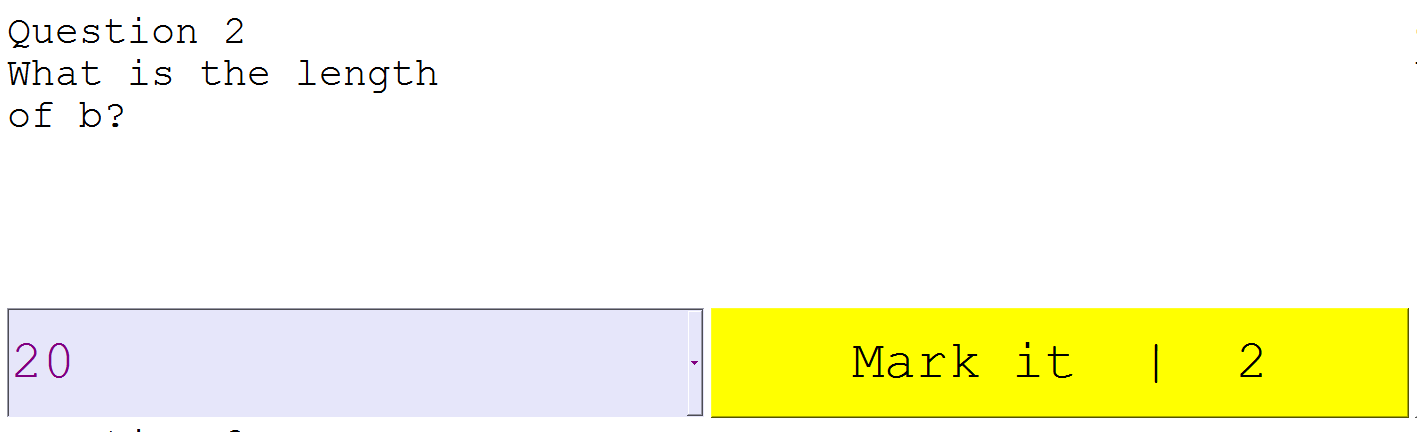
\includegraphics[width=\textwidth]{U:/git/COMP4Coursework2/Testing/screen_18}
\end{figure}

\textit{Mark it button is clicked: }

\begin{figure}[H]
    \label{fig: Second Screen}\caption{Second screen}
    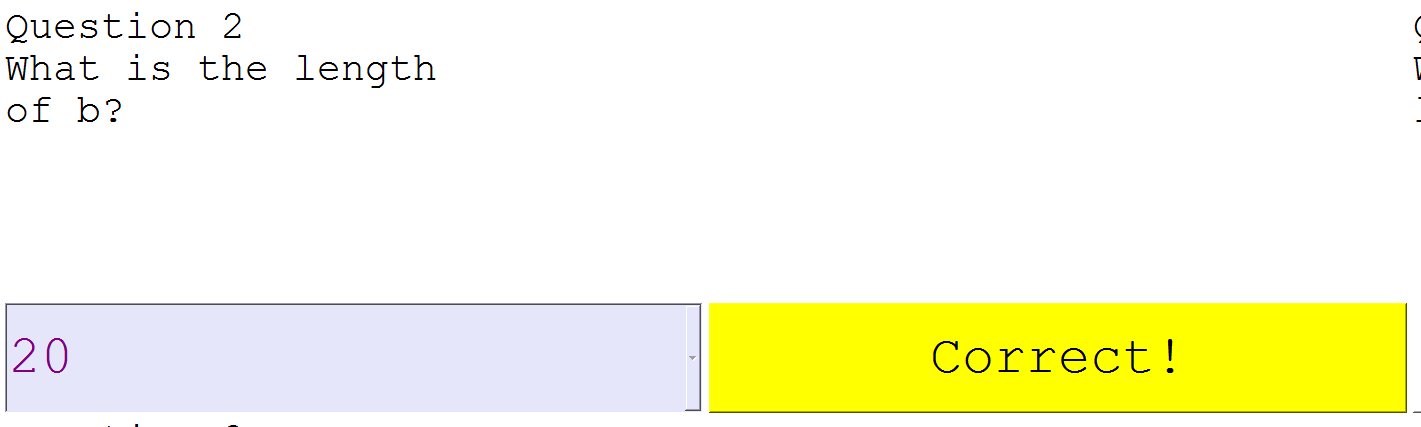
\includegraphics[width=\textwidth]{U:/git/COMP4Coursework2/Testing/screen_19}
\end{figure}

\textbf{Test 1.140}

\begin{figure}[H]
    \label{fig: First Screen}\caption{First screen}
    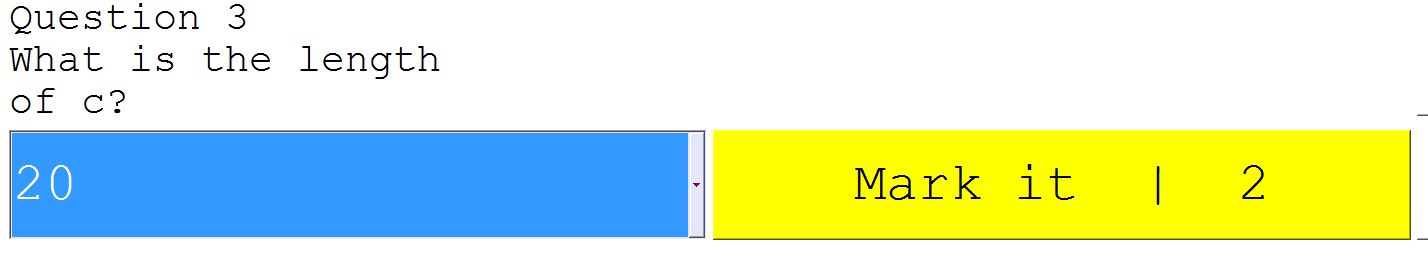
\includegraphics[width=\textwidth]{U:/git/COMP4Coursework2/Testing/screen_20}
\end{figure}

\textit{Mark it button is clicked: }

\begin{figure}[H]
    \label{fig: Second Screen}\caption{Second screen}
    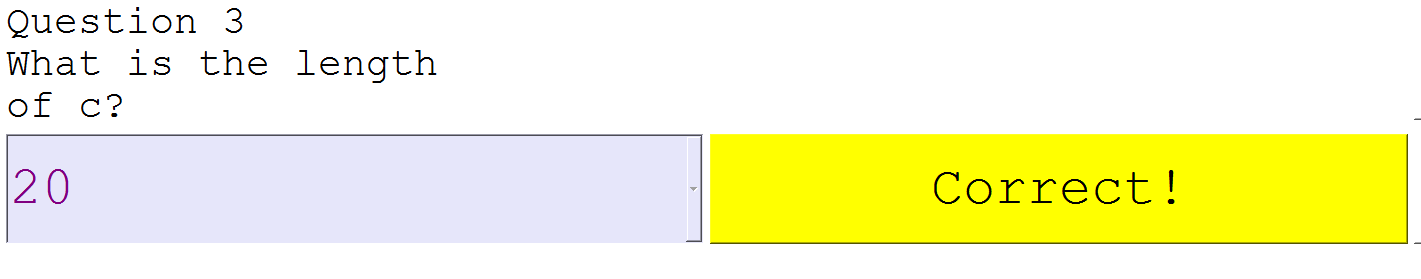
\includegraphics[width=\textwidth]{U:/git/COMP4Coursework2/Testing/screen_21}
\end{figure}

\textbf{Test 1.141}

\begin{figure}[H]
    \label{fig: Second Screen}\caption{Second screen}
    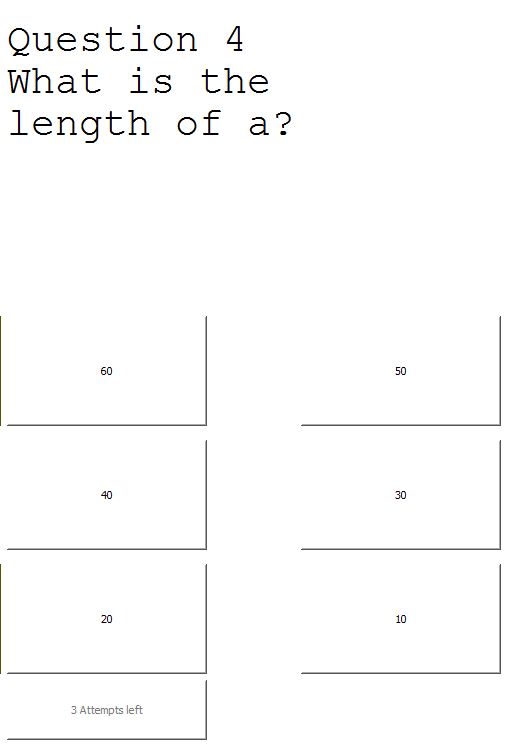
\includegraphics[width=\textwidth]{U:/git/COMP4Coursework2/Testing/screen_22}
\end{figure}

\textit{Wrong button is clicked - incorrect message}

\begin{figure}[H]
    \label{fig: Second Screen}\caption{Second screen}
    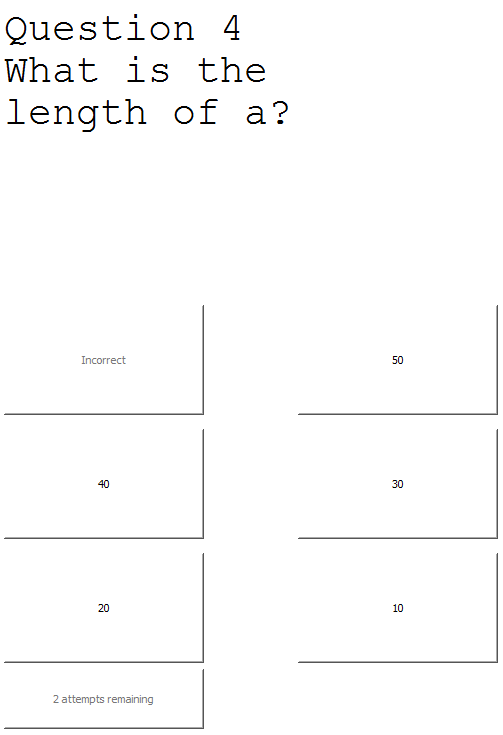
\includegraphics[width=\textwidth]{U:/git/COMP4Coursework2/Testing/screen_23}
\end{figure}

\textit{Right button is clicked - correct message}

\begin{figure}[H]
    \label{fig: Second Screen}\caption{Second screen}
    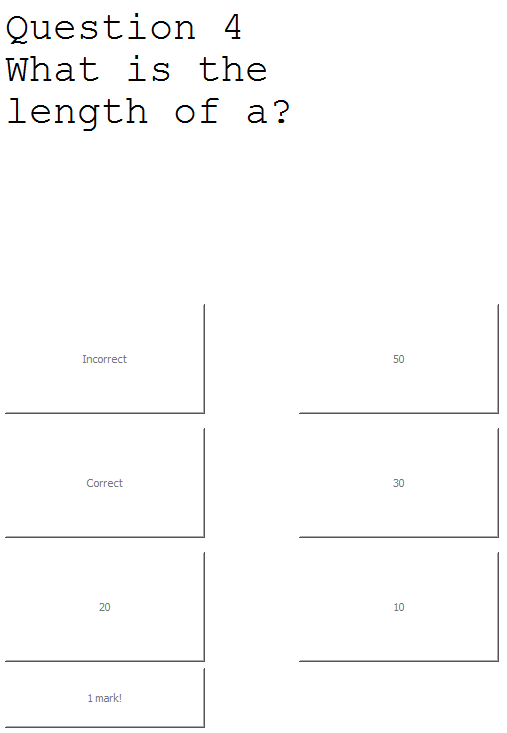
\includegraphics[width=\textwidth]{U:/git/COMP4Coursework2/Testing/screen_24}
\end{figure}

\textbf{Test 1.142}

\begin{figure}[H]
    \label{fig: First Screen}\caption{First screen}
    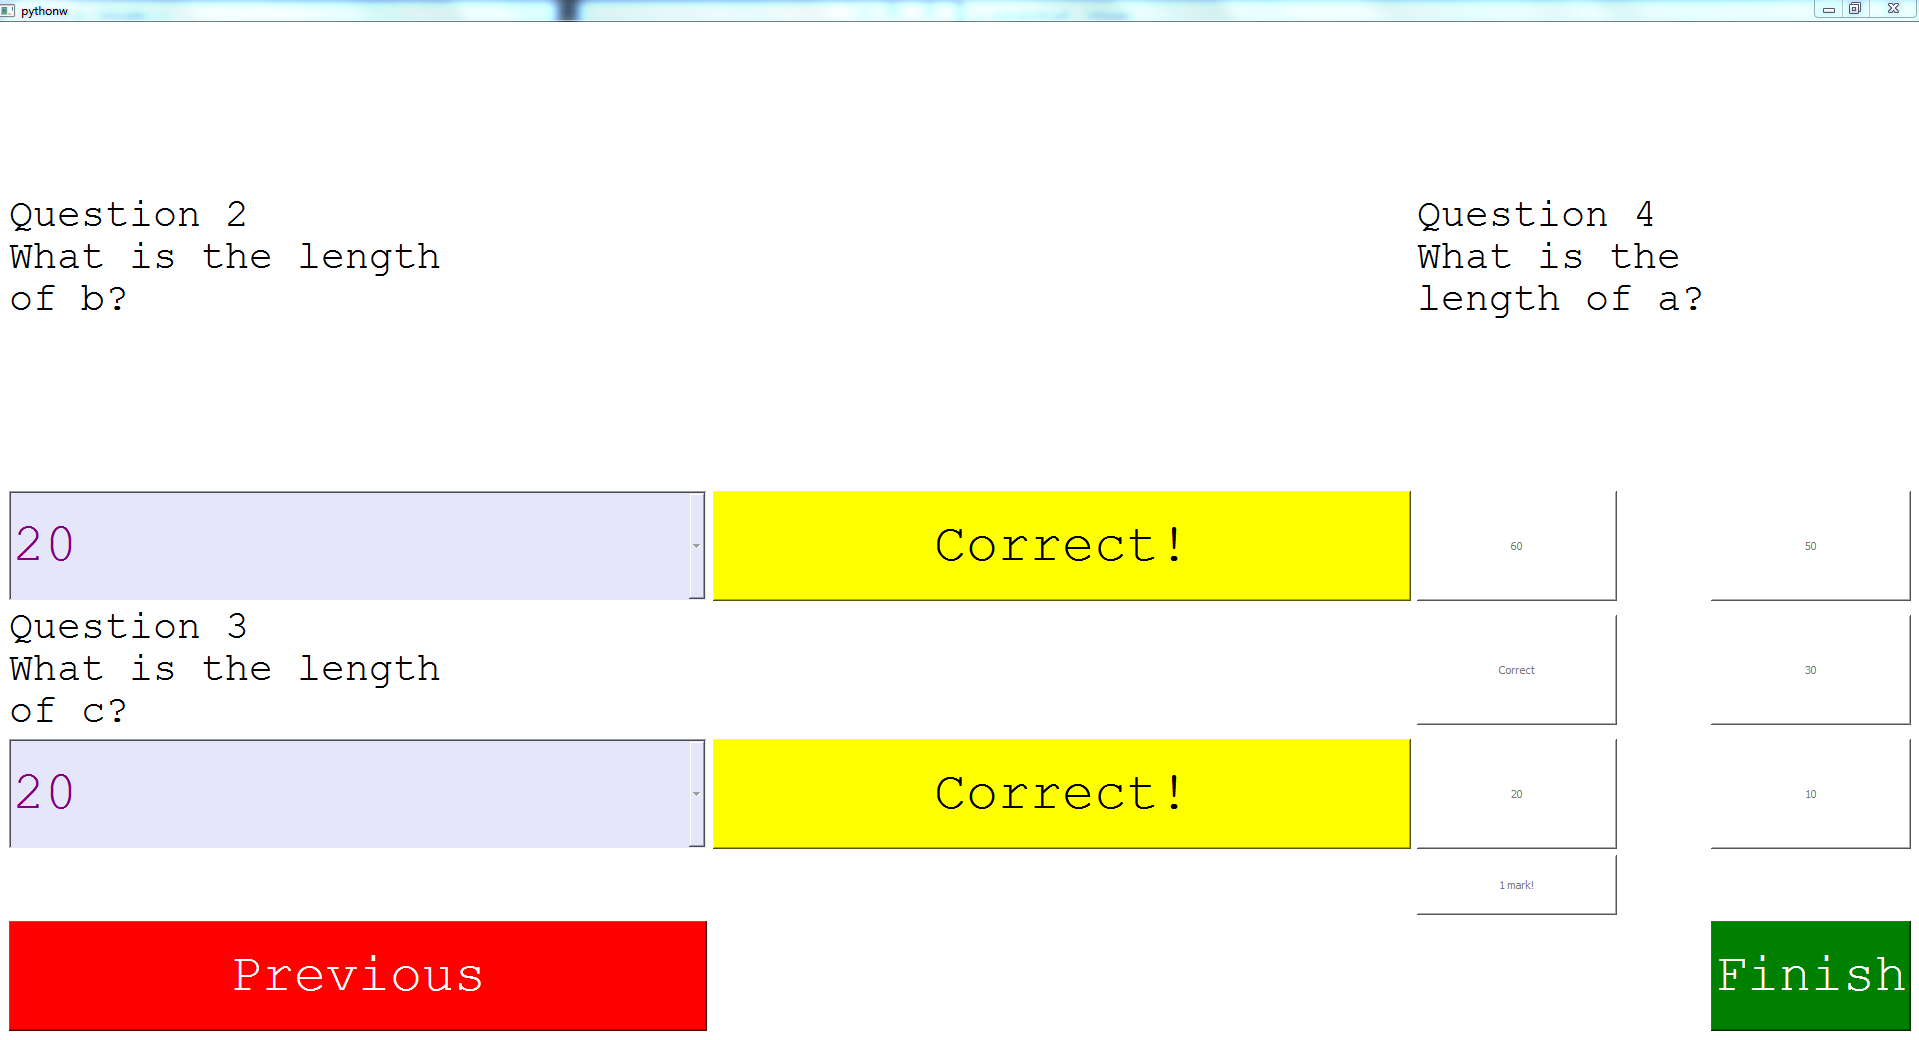
\includegraphics[width=\textwidth]{U:/git/COMP4Coursework2/Testing/screen_10}
\end{figure}

\textit{Previous button is clicked: }

\begin{figure}[H]
    \label{fig: Second Screen}\caption{Second screen}
    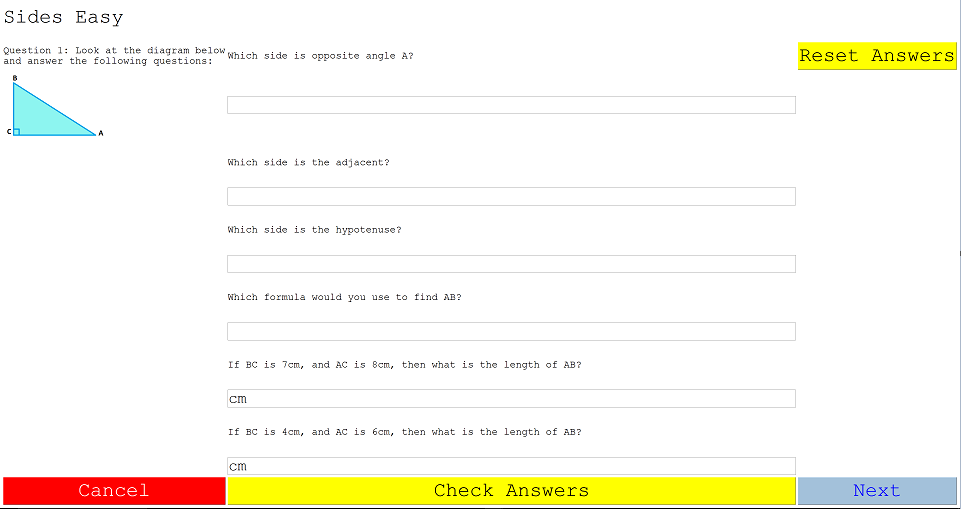
\includegraphics[width=\textwidth]{U:/git/COMP4Coursework2/Testing/screen_9}
\end{figure}

\textbf{Test 1.143}

\begin{figure}[H]
    \label{fig: First Screen}\caption{First screen}
    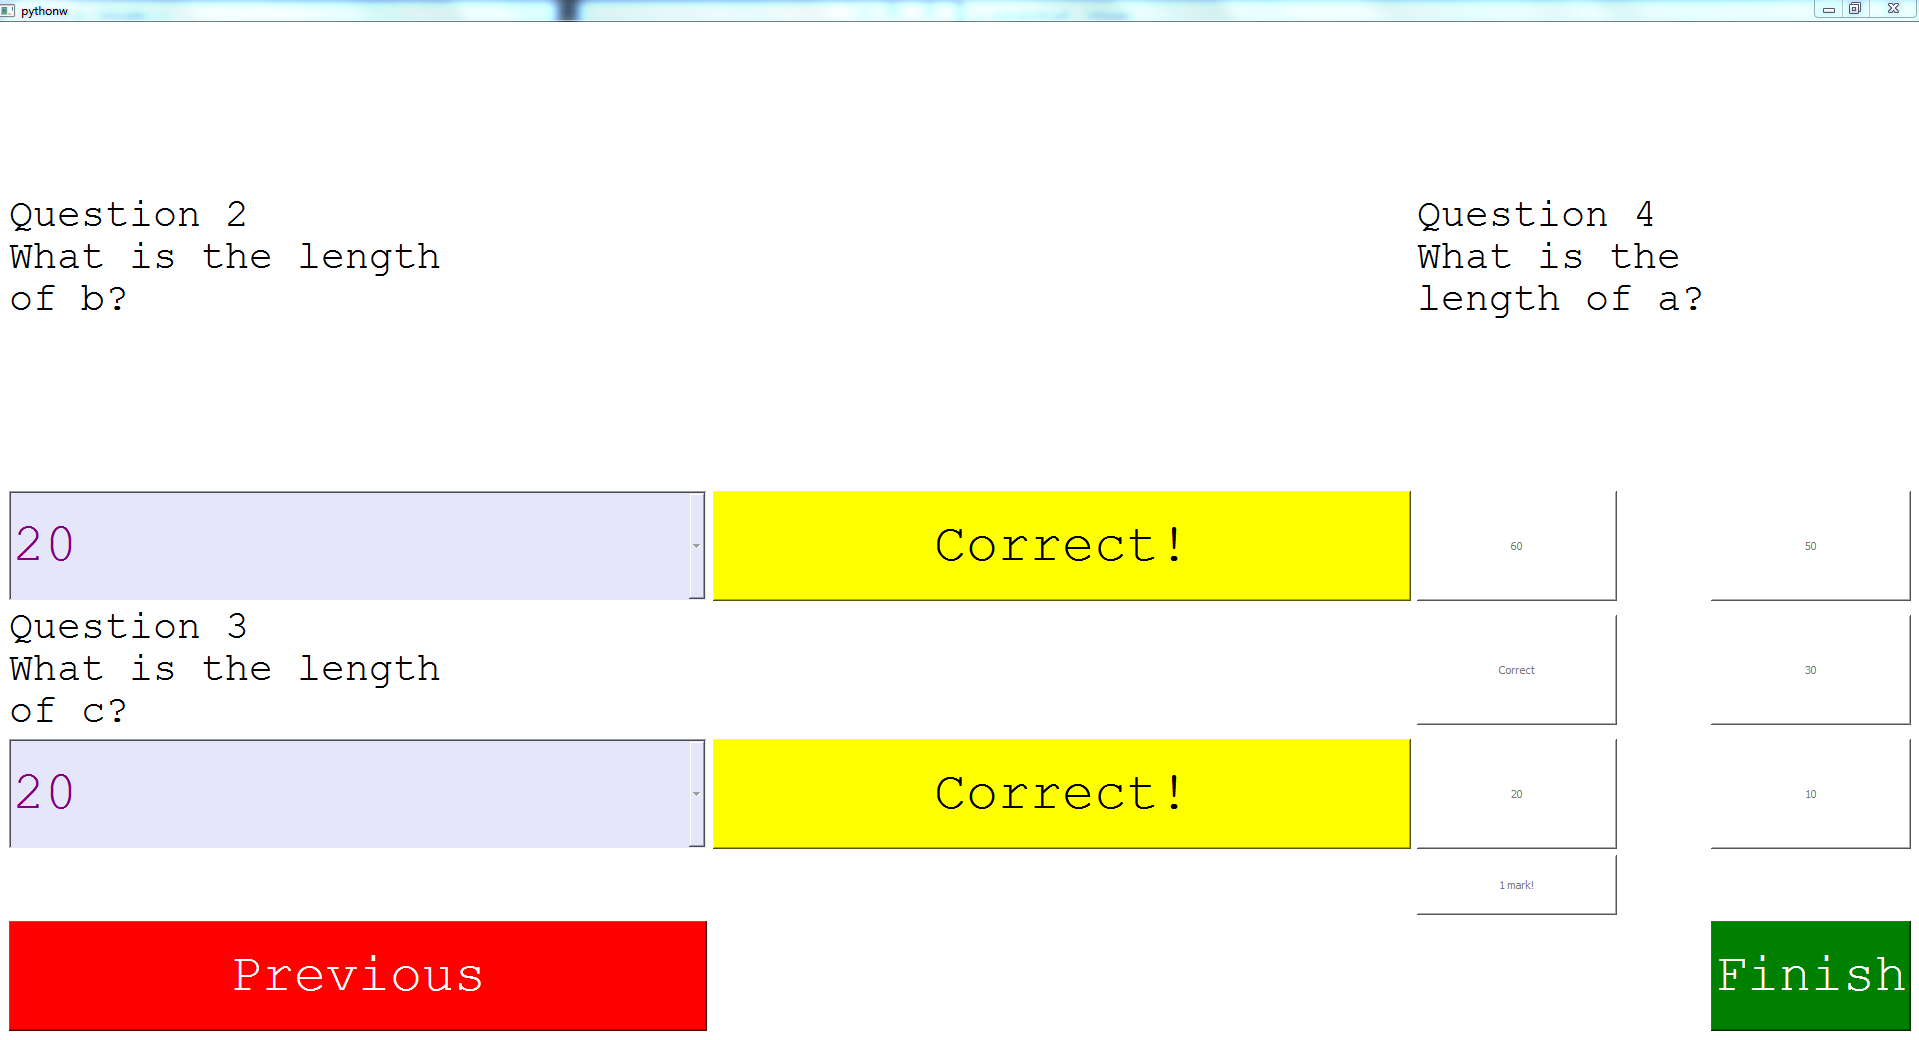
\includegraphics[width=\textwidth]{U:/git/COMP4Coursework2/Testing/screen_10}
\end{figure}

\textit{Finish button is clicked: }

\begin{figure}[H]
    \label{fig: Second Screen}\caption{Second screen}
    \includegraphics[width=\textwidth]{U:/git/COMP4Coursework2/Testing/screen_8}
\end{figure}

\textbf{Test 1.380}

\begin{figure}[H]
    \label{fig: First Screen}\caption{First screen}
    \includegraphics[width=\textwidth]{U:/git/COMP4Coursework2/Testing/screen_11}
\end{figure}

\textit{Return button is clicked: }

\begin{figure}[H]
    \label{fig: Second Screen}\caption{Second screen}
    \includegraphics[width=\textwidth]{U:/git/COMP4Coursework2/Testing/screen_2}
\end{figure}

\textbf{Test 1.431}

\begin{figure}[H]
    \label{fig: First Screen}\caption{First screen}
    \includegraphics[width=\textwidth]{U:/git/COMP4Coursework2/Testing/screen_12}
\end{figure}

\textit{Return button is clicked: }

\begin{figure}[H]
    \label{fig: Second Screen}\caption{Second screen}
    \includegraphics[width=\textwidth]{U:/git/COMP4Coursework2/Testing/screen_11}
\end{figure}

\textbf{Test 1.432}

\begin{figure}[H]
    \label{fig: First Screen}\caption{First screen}
    \includegraphics[width=\textwidth]{U:/git/COMP4Coursework2/Testing/screen_25}
\end{figure}

\textit{Query button is clicked: }

\begin{figure}[H]
    \label{fig: Second Screen}\caption{Second screen}
    \includegraphics[width=\textwidth]{U:/git/COMP4Coursework2/Testing/screen_26}
\end{figure}

\textbf{Test 1.441}

\begin{figure}[H]
    \label{fig: First Screen}\caption{First screen}
    \includegraphics[width=\textwidth]{U:/git/COMP4Coursework2/Testing/screen_1}
\end{figure}

\textit{Continue button is clicked: }

\begin{figure}[H]
    \label{fig: Second Screen}\caption{Second screen}
    \includegraphics[width=\textwidth]{U:/git/COMP4Coursework2/Testing/screen_2}
\end{figure}

\textbf{Test 1.442}

\begin{figure}[H]
    \label{fig: First Screen}\caption{First screen}
    \includegraphics[width=\textwidth]{U:/git/COMP4Coursework2/Testing/screen_11}
\end{figure}

\textit{Report button is clicked: }

\begin{figure}[H]
    \label{fig: Second Screen}\caption{Second screen}
    \includegraphics[width=\textwidth]{U:/git/COMP4Coursework2/Testing/screen_12}
\end{figure}

\textbf{Test 2.003}

\textit{Input is incorrect: }

\begin{figure}[H]
    \label{fig: Second Screen}\caption{Incorrect input}
    \includegraphics[width=\textwidth]{U:/git/COMP4Coursework2/Testing/screen_27}
\end{figure}

\textit{Input is correct: }

\begin{figure}[H]
    \label{fig: Second Screen}\caption{Second Correct input}
    \includegraphics[width=\textwidth]{U:/git/COMP4Coursework2/Testing/screen_28}
\end{figure}

\textbf{Tests 2.016, 2.017, 2.018, 2.019, 2.020, 2.021}

\textit{Input is incorrect: }

\begin{figure}[H]
    \label{fig: Second Screen}\caption{Incorrect inputs}
    \includegraphics[width=\textwidth]{U:/git/COMP4Coursework2/Testing/screen_29}
\end{figure}

\textit{Input is correct: }

\begin{figure}[H]
    \label{fig: Second Screen}\caption{Correct inputs}
    \includegraphics[width=\textwidth]{U:/git/COMP4Coursework2/Testing/screen_30}
\end{figure}

\textbf{Test 2.022}

\textit{Input is incorrect: }

\begin{figure}[H]
    \label{fig: Second Screen}\caption{Incorrect input}
    \includegraphics[width=\textwidth]{U:/git/COMP4Coursework2/Testing/screen_31}
\end{figure}

\textit{Input is correct: }

\begin{figure}[H]
    \label{fig: Second Screen}\caption{Correct input}
    \includegraphics[width=\textwidth]{U:/git/COMP4Coursework2/Testing/screen_32}
\end{figure}

\textbf{Test 2.023}

\textit{Input is incorrect: }

\begin{figure}[H]
    \label{fig: Second Screen}\caption{Incorrect input}
    \includegraphics[width=\textwidth]{U:/git/COMP4Coursework2/Testing/screen_33}
\end{figure}

\textit{Input is correct: }

\begin{figure}[H]
    \label{fig: Second Screen}\caption{Correct input}
    \includegraphics[width=\textwidth]{U:/git/COMP4Coursework2/Testing/screen_34}
\end{figure}

\textbf{Test 2.024}

\textit{Input is incorrect: }

\begin{figure}[H]
    \label{fig: Second Screen}\caption{Incorrect input}
    \includegraphics[width=\textwidth]{U:/git/COMP4Coursework2/Testing/screen_23}
\end{figure}

\textit{Input is correct: }

\begin{figure}[H]
    \label{fig: Second Screen}\caption{Correct input}
    \includegraphics[width=\textwidth]{U:/git/COMP4Coursework2/Testing/screen_24}
\end{figure}

\textbf{Test 2.295}

\textit{Task is selected to query: }

\begin{figure}[H]
    \label{fig: Second Screen}\caption{Task queried}
    \includegraphics[width=\textwidth]{U:/git/COMP4Coursework2/Testing/screen_35}
\end{figure}

\textbf{Test 2.296}

\textit{Score is selected to query: }

\begin{figure}[H]
    \label{fig: Second Screen}\caption{Score queried}
    \includegraphics[width=\textwidth]{U:/git/COMP4Coursework2/Testing/screen_36}
\end{figure}

\textbf{Test 3.009}

\textit{Task name is stored under the task name header: }

\begin{figure}[H]
    \label{fig: Second Screen}\caption{Task name stored}
    \includegraphics[width=\textwidth]{U:/git/COMP4Coursework2/Testing/screen_37}
\end{figure}

\textbf{Test 3.011}

\textit{The scores are stored under the score headers: }

\begin{figure}[H]
    \label{fig: Second Screen}\caption{Scores stored}
    \includegraphics[width=\textwidth]{U:/git/COMP4Coursework2/Testing/screen_38}
\end{figure}

\textbf{Test 4.015}

\textit{Incorrect answer output: }

\begin{figure}[H]
    \label{fig: Second Screen}\caption{Incorrect answer}
    \includegraphics[width=\textwidth]{U:/git/COMP4Coursework2/Testing/screen_39}
\end{figure}

\textit{Correct answer output: }

\begin{figure}[H]
    \label{fig: Second Screen}\caption{Correct answer}
    \includegraphics[width=\textwidth]{U:/git/COMP4Coursework2/Testing/screen_40}
\end{figure}

\textit{No answer output: }

\begin{figure}[H]
    \label{fig: Second Screen}\caption{Absent answer}
    \includegraphics[width=\textwidth]{U:/git/COMP4Coursework2/Testing/screen_41}
\end{figure}

\textbf{Test 4.016}

\textit{Incorrect answer output: }

\begin{figure}[H]
    \label{fig: Second Screen}\caption{Incorrect answer}
    \includegraphics[width=\textwidth]{U:/git/COMP4Coursework2/Testing/screen_42}
\end{figure}

\textit{Correct answer output: }

\begin{figure}[H]
    \label{fig: Second Screen}\caption{Correct answer}
    \includegraphics[width=\textwidth]{U:/git/COMP4Coursework2/Testing/screen_43}
\end{figure}

\textit{No answer output: }

\begin{figure}[H]
    \label{fig: Second Screen}\caption{Absent answer}
    \includegraphics[width=\textwidth]{U:/git/COMP4Coursework2/Testing/screen_44}
\end{figure}

\textbf{Test 4.017}

\textit{Incorrect answer output: }

\begin{figure}[H]
    \label{fig: Second Screen}\caption{Incorrect answer}
    \includegraphics[width=\textwidth]{U:/git/COMP4Coursework2/Testing/screen_45}
\end{figure}

\textit{Correct answer output: }

\begin{figure}[H]
    \label{fig: Second Screen}\caption{Correct answer}
    \includegraphics[width=\textwidth]{U:/git/COMP4Coursework2/Testing/screen_46}
\end{figure}

\textit{No answer output: }

\begin{figure}[H]
    \label{fig: Second Screen}\caption{Absent answer}
    \includegraphics[width=\textwidth]{U:/git/COMP4Coursework2/Testing/screen_44}
\end{figure}

\textbf{Test 4.018}

\textit{Before resetting: }

\begin{figure}[H]
    \label{fig: Second Screen}\caption{Before reset}
    \includegraphics[width=\textwidth]{U:/git/COMP4Coursework2/Testing/screen_48}
\end{figure}

\textit{After resetting: }

\begin{figure}[H]
    \label{fig: Second Screen}\caption{After reset}
    \includegraphics[width=\textwidth]{U:/git/COMP4Coursework2/Testing/screen_49}
\end{figure}

\textbf{Test 5.001}

\textbf{Test 5.003}

\textit{The information is being stored in the right place here: }

\begin{figure}[H]
    \label{fig: Second Screen}\caption{Database}
    \includegraphics[width=\textwidth]{U:/git/COMP4Coursework2/Testing/screen_50}
\end{figure}

\textbf{Test 5.004}

\textit{The right amount of information is being stored here: }

\begin{figure}[H]
    \label{fig: Second Screen}\caption{Database}
    \includegraphics[width=\textwidth]{U:/git/COMP4Coursework2/Testing/screen_50}
\end{figure}

\textbf{Test 5.006}

\textit{No illegitimate information is stored here: }

\begin{figure}[H]
    \label{fig: Second Screen}\caption{Database}
    \includegraphics[width=\textwidth]{U:/git/COMP4Coursework2/Testing/screen_50}
\end{figure}

\section{Evaluation}

\subsection{Approach to Testing}

I decided to use a variation of testing methods in order to ensure that every aspect of this system works adequately and robustly, and meets as many client specifications as possible. For example, top-down testing was used to check that every button in the system works as intended, bottum up testing was used to test each input opportunity as they were created, black box testing was used to make sure all information was stored in the database correctly, white box testing was used to test each of the marking algorithm in the system worked efficiently, and finally acceptance testing was used to make sure that the client was satisfied with the system. For test series 1, not every button test was documented because there are too many of them and most of them share parent code, so testing at least one of each child button or unique button was enough to be sure that the same code was working everywhere.

\subsection{Problems Encountered}

\begin{itemize}
\item Initially, on the report widget, I tried to have a separate window pop up to output the results of the user's query, however I struggled to get some of the data variables to pass between files, so I had to have the QTableWidget on the same screen as the query menu. However, this turned out to be just as effective as the first attempted method.

\item For the generic question 4 on the homeworks, I wanted to put in drag and drop functionality to provide a variation of input types. However, there was a very unusual error where enabling a built in drag function would break the entire program, and it was beyond my abilities to either solve this problem, or find another way to implement the drag and drop functionality. So I replaced the drag and drop idea with multiple choice buttons, which admittedly is not as technically 'good', but there is still a range of input types, and this replacement works efficiently.

\item There was a significant problem with saving results to the database; I could not generate a total score variable because, again, I could not find how to pass the required variables across files, as the first and second screen's code are separate from each other. As a result of this, I could not store a Rating variable either, so I resorted to just including the task name along with each questions score.

\item The biggest problem was finding a way to create separate accounts, all accessible from different computers in a LAN, and having an administrator account capable of setting homeworks. It occured to me that this was far too much to code in the time I had, and that I had bitten off much more than I could chew, so I reformed the program down to a single user, self-assessing program, which still records data, but that data stays on one machine, used by one person. More than one person can use it; it can be installed  on multiple offline machines, of course. The client will not be able to keep track of progress, they will have to rely on users to be honest or provide evidence.

\item The database kept having to be over-written, and would only hold one record, otherwise it would crash, if you tried to record results for the same task twice. I fixed this by implementing some SQL code which would fetch all information currently in the database and check to see if any records with the same TaskName value existed already. If so, another SQL statement would check the values of the current scores and the new scores and only overwrite them if the new ones were higher. Otherwise it would record the new task entirely. Now it works; there are no circumstances or results which would cause the program to crash upon attempting to record them. Either a new record is saved or an old one is overwritten.

\end{itemize}

\subsection{Strengths of Testing}

The main strength of my testing was testing the answer marking algorithms; these algorithms included awarding marks, removing remaining attempts and disabling buttons, and after testing every possible input, each of these algorithms works robustly and exactly how they were intended. Any wrong data type inputs are dealt with using error messages, and the buttons would be disabled after losing all attempts or getting the correct answer to prevent the user being able to attempt the same question more than once, overwrite the content of the buttons and crash the system upon trying to save information to the database. This also leads to the next strength, the bottum up input testing, as this also shows that no input can cause the program to crash at any point.

\subsection{Weaknesses of Testing}

The main weakness of my testing was simply the massive number of buttons which had to be tested. All of them were tested, and all of them work, even after up to three different methods of coding them, and most of them have a parent class, so the same code works in each place. This was a weakness because it took time, and not every test could be documented, as they were essentially the same. The other weakness of testing is the acceptance testing; after cutting out the entire administrator aspect of the program as well as LAN capabilites, it is unlikely that the client will be fully satisfied. With luck, they accept the system anyway, as it does meet some other main specifications.

\subsection{Reliability of Application}

My system is more or less reliable; all data stored is accurate and correct, and is stored in the right quantity. There are no validation errors when checking answers, as they are hard-coded, and testing has proven the algorithms reliable under every circumstance. The information in the lessons is correct, and all of the buttons work exactly as intended. Only one potentially system breaking issue was found, where the database could not save the same task twice, but that problem has been solved. Finally, the data in the database can only be manipulated by completing a task, there is no way to manually enter the database and change the data.

\subsection{Robustness of Application}

My program is very robust; there are error messages for every possible error, including wrong data types, or not being able to progress. The only error which pops up pretty much every time a new screen opens is the word \_raise() not being recognised, however that makes absolutely no difference to anything and can be dealt with simply by putting in an error exception in every place where it could occur. There is no point in the program where an infinite loop can be entered.

